% Options for packages loaded elsewhere
\PassOptionsToPackage{unicode}{hyperref}
\PassOptionsToPackage{hyphens}{url}
%
\documentclass[
  12pt,
]{book}
\usepackage{amsmath,amssymb}
\usepackage{iftex}
\ifPDFTeX
  \usepackage[T1]{fontenc}
  \usepackage[utf8]{inputenc}
  \usepackage{textcomp} % provide euro and other symbols
\else % if luatex or xetex
  \usepackage{unicode-math} % this also loads fontspec
  \defaultfontfeatures{Scale=MatchLowercase}
  \defaultfontfeatures[\rmfamily]{Ligatures=TeX,Scale=1}
\fi
\usepackage{lmodern}
\ifPDFTeX\else
  % xetex/luatex font selection
\fi
% Use upquote if available, for straight quotes in verbatim environments
\IfFileExists{upquote.sty}{\usepackage{upquote}}{}
\IfFileExists{microtype.sty}{% use microtype if available
  \usepackage[]{microtype}
  \UseMicrotypeSet[protrusion]{basicmath} % disable protrusion for tt fonts
}{}
\makeatletter
\@ifundefined{KOMAClassName}{% if non-KOMA class
  \IfFileExists{parskip.sty}{%
    \usepackage{parskip}
  }{% else
    \setlength{\parindent}{0pt}
    \setlength{\parskip}{6pt plus 2pt minus 1pt}}
}{% if KOMA class
  \KOMAoptions{parskip=half}}
\makeatother
\usepackage{xcolor}
\usepackage{color}
\usepackage{fancyvrb}
\newcommand{\VerbBar}{|}
\newcommand{\VERB}{\Verb[commandchars=\\\{\}]}
\DefineVerbatimEnvironment{Highlighting}{Verbatim}{commandchars=\\\{\}}
% Add ',fontsize=\small' for more characters per line
\usepackage{framed}
\definecolor{shadecolor}{RGB}{248,248,248}
\newenvironment{Shaded}{\begin{snugshade}}{\end{snugshade}}
\newcommand{\AlertTok}[1]{\textcolor[rgb]{0.94,0.16,0.16}{#1}}
\newcommand{\AnnotationTok}[1]{\textcolor[rgb]{0.56,0.35,0.01}{\textbf{\textit{#1}}}}
\newcommand{\AttributeTok}[1]{\textcolor[rgb]{0.13,0.29,0.53}{#1}}
\newcommand{\BaseNTok}[1]{\textcolor[rgb]{0.00,0.00,0.81}{#1}}
\newcommand{\BuiltInTok}[1]{#1}
\newcommand{\CharTok}[1]{\textcolor[rgb]{0.31,0.60,0.02}{#1}}
\newcommand{\CommentTok}[1]{\textcolor[rgb]{0.56,0.35,0.01}{\textit{#1}}}
\newcommand{\CommentVarTok}[1]{\textcolor[rgb]{0.56,0.35,0.01}{\textbf{\textit{#1}}}}
\newcommand{\ConstantTok}[1]{\textcolor[rgb]{0.56,0.35,0.01}{#1}}
\newcommand{\ControlFlowTok}[1]{\textcolor[rgb]{0.13,0.29,0.53}{\textbf{#1}}}
\newcommand{\DataTypeTok}[1]{\textcolor[rgb]{0.13,0.29,0.53}{#1}}
\newcommand{\DecValTok}[1]{\textcolor[rgb]{0.00,0.00,0.81}{#1}}
\newcommand{\DocumentationTok}[1]{\textcolor[rgb]{0.56,0.35,0.01}{\textbf{\textit{#1}}}}
\newcommand{\ErrorTok}[1]{\textcolor[rgb]{0.64,0.00,0.00}{\textbf{#1}}}
\newcommand{\ExtensionTok}[1]{#1}
\newcommand{\FloatTok}[1]{\textcolor[rgb]{0.00,0.00,0.81}{#1}}
\newcommand{\FunctionTok}[1]{\textcolor[rgb]{0.13,0.29,0.53}{\textbf{#1}}}
\newcommand{\ImportTok}[1]{#1}
\newcommand{\InformationTok}[1]{\textcolor[rgb]{0.56,0.35,0.01}{\textbf{\textit{#1}}}}
\newcommand{\KeywordTok}[1]{\textcolor[rgb]{0.13,0.29,0.53}{\textbf{#1}}}
\newcommand{\NormalTok}[1]{#1}
\newcommand{\OperatorTok}[1]{\textcolor[rgb]{0.81,0.36,0.00}{\textbf{#1}}}
\newcommand{\OtherTok}[1]{\textcolor[rgb]{0.56,0.35,0.01}{#1}}
\newcommand{\PreprocessorTok}[1]{\textcolor[rgb]{0.56,0.35,0.01}{\textit{#1}}}
\newcommand{\RegionMarkerTok}[1]{#1}
\newcommand{\SpecialCharTok}[1]{\textcolor[rgb]{0.81,0.36,0.00}{\textbf{#1}}}
\newcommand{\SpecialStringTok}[1]{\textcolor[rgb]{0.31,0.60,0.02}{#1}}
\newcommand{\StringTok}[1]{\textcolor[rgb]{0.31,0.60,0.02}{#1}}
\newcommand{\VariableTok}[1]{\textcolor[rgb]{0.00,0.00,0.00}{#1}}
\newcommand{\VerbatimStringTok}[1]{\textcolor[rgb]{0.31,0.60,0.02}{#1}}
\newcommand{\WarningTok}[1]{\textcolor[rgb]{0.56,0.35,0.01}{\textbf{\textit{#1}}}}
\usepackage{longtable,booktabs,array}
\usepackage{calc} % for calculating minipage widths
% Correct order of tables after \paragraph or \subparagraph
\usepackage{etoolbox}
\makeatletter
\patchcmd\longtable{\par}{\if@noskipsec\mbox{}\fi\par}{}{}
\makeatother
% Allow footnotes in longtable head/foot
\IfFileExists{footnotehyper.sty}{\usepackage{footnotehyper}}{\usepackage{footnote}}
\makesavenoteenv{longtable}
\usepackage{graphicx}
\makeatletter
\def\maxwidth{\ifdim\Gin@nat@width>\linewidth\linewidth\else\Gin@nat@width\fi}
\def\maxheight{\ifdim\Gin@nat@height>\textheight\textheight\else\Gin@nat@height\fi}
\makeatother
% Scale images if necessary, so that they will not overflow the page
% margins by default, and it is still possible to overwrite the defaults
% using explicit options in \includegraphics[width, height, ...]{}
\setkeys{Gin}{width=\maxwidth,height=\maxheight,keepaspectratio}
% Set default figure placement to htbp
\makeatletter
\def\fps@figure{htbp}
\makeatother
\setlength{\emergencystretch}{3em} % prevent overfull lines
\providecommand{\tightlist}{%
  \setlength{\itemsep}{0pt}\setlength{\parskip}{0pt}}
\setcounter{secnumdepth}{5}
\usepackage{booktabs}
\ifLuaTeX
  \usepackage{selnolig}  % disable illegal ligatures
\fi
\usepackage[]{natbib}
\bibliographystyle{apalike}
\IfFileExists{bookmark.sty}{\usepackage{bookmark}}{\usepackage{hyperref}}
\IfFileExists{xurl.sty}{\usepackage{xurl}}{} % add URL line breaks if available
\urlstyle{same}
\hypersetup{
  pdftitle={Introduction to Term Structure Models},
  pdfauthor={Alain Monfort and Jean-Paul Renne},
  hidelinks,
  pdfcreator={LaTeX via pandoc}}

\title{Introduction to Term Structure Models}
\author{Alain Monfort and Jean-Paul Renne}
\date{2024-02-07}

\usepackage{amsthm}
\newtheorem{theorem}{Theorem}[chapter]
\newtheorem{lemma}{Lemma}[chapter]
\newtheorem{corollary}{Corollary}[chapter]
\newtheorem{proposition}{Proposition}[chapter]
\newtheorem{conjecture}{Conjecture}[chapter]
\theoremstyle{definition}
\newtheorem{definition}{Definition}[chapter]
\theoremstyle{definition}
\newtheorem{example}{Example}[chapter]
\theoremstyle{definition}
\newtheorem{exercise}{Exercise}[chapter]
\theoremstyle{definition}
\newtheorem{hypothesis}{Hypothesis}[chapter]
\theoremstyle{remark}
\newtheorem*{remark}{Remark}
\newtheorem*{solution}{Solution}
\begin{document}
\maketitle

{
\setcounter{tocdepth}{1}
\tableofcontents
}
\newcommand{\bv}[1]{\mathbf{#1}}

\hypertarget{intro}{%
\chapter*{Introduction to Term Structure Models}\label{intro}}

Modeling dynamic term structures serves as a practical and indispensable tool in the realm of finance. It enables investors, institutions, and policymakers to make informed decisions, manage risk effectively, and allocate resources wisely. By understanding how interest rates and yields evolve over time, these models offer a clear lens through which to assess market trends and price financial instruments accurately.

This course has been developed by \href{https://faculty.crest.fr/amonfort/}{Alain Monfort} and \href{https://sites.google.com/site/jeanpaulrenne/home}{Jean-Paul Renne}. It is illustrated by R codes using various packages that can be obtained from \href{https://cran.r-project.org}{CRAN}. This \texttt{TSModels} package is available on GitHub. To install it, one need to employ the \texttt{devtools} library:

\begin{Shaded}
\begin{Highlighting}[]
\FunctionTok{install.packages}\NormalTok{(}\StringTok{"devtools"}\NormalTok{) }\CommentTok{\# needed to use "install\_github"}
\FunctionTok{library}\NormalTok{(devtools)}
\FunctionTok{install\_github}\NormalTok{(}\StringTok{"jrenne/TSModels"}\NormalTok{)}
\FunctionTok{library}\NormalTok{(AEC)}
\end{Highlighting}
\end{Shaded}

\textbf{Useful (R) links:}

\begin{itemize}
\item
  Download R:

  \begin{enumerate}
  \def\labelenumi{\alph{enumi}.}
  \tightlist
  \item
    R software: \url{https://cran.r-project.org} (the basic R software)
  \item
    RStudio: \url{https://www.rstudio.com} (a convenient R editor)
  \end{enumerate}
\item
  Tutorials:

  \begin{enumerate}
  \def\labelenumi{\alph{enumi}.}
  \tightlist
  \item
    Rstudio: \url{https://dss.princeton.edu/training/RStudio101.pdf} (by Oscar Torres-Reyna)
  \item
    R: \url{https://cran.r-project.org/doc/contrib/Paradis-rdebuts_en.pdf} (by Emmanuel Paradis)
  \end{enumerate}
\end{itemize}

\hypertarget{ChapterAffine}{%
\chapter{Affine processes}\label{ChapterAffine}}

\hypertarget{Information}{%
\section{Information in the Economy: The ``factors''}\label{Information}}

On each date \(t=1,2,\dots,T\), agents receive new information by observing \emph{factors}, also called \emph{states}. We denote the (\(K\)-dimensional) vector of factors by \(w_t\). Vector \(w_t\) is usually random. On date \(t\), vector \(w_t\) is supposed to be perfectly observed by the agents (investors), but can be only partially observed, or unobserved by the econometrician.

Naturally, \(w_t\) can be decomposed into different sub-vectors of different natures. For instance, we can have \(w_t = (y_t', z_t')'\) with

\begin{itemize}
\tightlist
\item
  \(y_t\): observable vector of (geometric) returns,
\item
  \(z_t\): regime, unobserved by the econometrician.
\end{itemize}

Some of the components of \(w_t\) can be prices. For instance, one component could be a short-term rate, a stock return, or an exchange rate. It can also include macroeconomic variables (inflation, GDP growth), or agent-specific variables.

\hypertarget{Dynamic}{%
\section{Dynamic models and Laplace transform (L.T.)}\label{Dynamic}}

The objective of a dynamic model is to describe the random changes in \(w_t\). The dynamics can be historical or risk-neutral (see Section \ref{PandQ}). The dynamics we consider are parametric, in the sense that the conditional distribution \(w_{t+1}|\underline{w_t}\) (with \(\underline{w_t}=\{w_t,w_{t-1},\dots\}\)) depends on a vector of parameters \(\theta\). In practice, it may be the case that \(\theta\) is unknown by the econometrician (see Section \ref{Estimation}).

The choice (or estimation) of a conditional distribution is equivalent to the choice (or estimation) of a conditional \emph{Laplace transforms}:
\begin{equation}
\varphi(u|\underline{w_t},\theta) =
\mathbb{E}_{\theta}[\exp(u'w_{t+1})|\underline{w_t}], \quad u \in \mathbb{R}^K,\label{eq:LT}
\end{equation}
or a conditional \emph{log Laplace transforms}:
\[
\psi(u|\underline{w_t},\theta) =
\log\{\mathbb{E}_{\theta}[\exp(u'w_{t+1})|\underline{w_t}]\}, \quad u \in
\mathbb{R}^K.
\]

\begin{example}[Conditionally Bernoulli process]
\protect\hypertarget{exm:exBenoulli}{}\label{exm:exBenoulli}If \(w_{t+1}|\underline{w_t} \sim {\mathcal{I}} [p(\underline{w_t},\theta)]\), then:
\[
\varphi(u|w_t)=
\mathbb{E}[\exp(u w_{t+1}) \mid \underline{w_t}] = p_t \exp(u) + 1-p_t
\]
with \(p_t = p(\underline{w_t}, \theta)\).
\end{example}

\begin{example}[Conditionally Binomial process]
\protect\hypertarget{exm:exBenoulli2}{}\label{exm:exBenoulli2}If \(w_{t+1}|\underline{w_t} \in {\mathcal{B}}(n, p_t)\), then:
\[
\varphi(u|w_t)=[p_t   \exp(u) + 1-p_t]^n.
\]
\end{example}

\begin{example}[Conditionally Poisson process]
\protect\hypertarget{exm:exPoisson}{}\label{exm:exPoisson}If \(w_{t+1}|\underline{w_t} \sim {\mathcal{P}}(\lambda_t)\), then:
\begin{eqnarray*}
\varphi(u|w_t) & =&   \sum^\infty_{j=0}  \dfrac{1}{j!}  \exp(-\lambda_t) \lambda^j_t   \exp(uj)  = \exp(-\lambda_t) \exp[\lambda_t \exp(u)] \\
& =& \exp\{\lambda_t[\exp(u)-1]\}.
\end{eqnarray*}
\end{example}

\begin{example}[Conditionally normal (or Gaussian) process]
\protect\hypertarget{exm:exGaussian}{}\label{exm:exGaussian}If \(w_{t+1}|\underline{w_t} \sim \mathcal{N}\left(m(\underline{w_t},\theta), \Sigma(\underline{w_t},\theta)\right)\), then:

\[
u'w_{t+1}|\underline{w_t} \sim \mathcal{N}\left(u'm(\underline{w_t},\theta), u'\Sigma(\underline{w_t},\theta)u\right),
\]
and, therefore:
\[
\left\{
\begin{array}{ccc}
\varphi(u|\underline{w_t},\theta) &=& \exp\left[u'm(\underline{w_t},\theta)+
\frac{1}{2} u'\Sigma(\underline{w_t},\theta)u\right]\\
\psi(u|\underline{w_t},\theta) &=&
u'm(\underline{w_t},\theta) +  \frac{1}{2}
u'\Sigma(\underline{w_t},\theta)u.
\end{array}
\right.
\]
\end{example}

\hypertarget{AffineLaplace}{%
\section{Laplace Transform and moments/cumulants}\label{AffineLaplace}}

Here are some properties of the Laplace transform, defined in \eqref{eq:LT}:

\begin{itemize}
\tightlist
\item
  \(\varphi(0|\underline{w_t},\theta) = 1\) and \(\psi(0|\underline{w_t},\theta)=0\).
\item
  It is defined in a convex set \(E\) (containing \(0\)).
\item
  If the interior of \(E\) is non empty, all the (conditional) moments exist.
\end{itemize}

As mentioned above, knowing the (conditional) Laplace transform is equivalent to knowing the (conditional) moments---if they exist. In the scalar case, we have that:

\begin{itemize}
\tightlist
\item
  the moment of order \(n\) closely relates to the \(n^{th}\) derivatives of \(\varphi\):
  \[
  \mathbb{E}_{\theta}[w^n_{t+1}|\underline{w_t}] = \left[ \begin{array}{l}  \dfrac{\partial^n
  \varphi(u|\underline{w_t},\theta)}{\partial u^n}
  \end{array} \right]_{u=0},
  \]
\item
  the cumulant of order \(n\) closely relates to the \(n^{th}\) derivatives of \(\psi\):
  \[
  K_n(\underline{w_t},\theta) = \left[ \begin{array}{l}  \dfrac{\partial^n
  \psi(u|\underline{w_t},\theta)}{\partial u^n}
  \end{array} \right]_{u=0}.
  \]
\end{itemize}

In particular, what precedes implies that:
\[
\left\{
\begin{array}{ccc}
K_1(\underline{w_t},\theta) &=& \mathbb{E}_{\theta}[w_{t+1}|\underline{w_t}]\\
K_2(\underline{w_t}, \theta) &=& \mathbb{V}ar_{\theta}[w_{t+1}|\underline{w_t}].
\end{array}
\right.
\]

Accordingly, \(\varphi\) and \(\psi\) are respectively called conditional \emph{moment}- and \emph{cumulant}-generating function.

In the multivariate case, we have:
\begin{eqnarray*}
\mathbb{E}_{\theta}[w_{t+1}|\underline{w_t}] &=& \left[\begin{array}{l}  \dfrac{\partial \psi}{\partial
u} (u|\underline{w_t},\theta)  \end{array} \right]_{u=0} \\
\mathbb{V}ar_{\theta}[w_{t+1}|\underline{w_t}] &=& \left[\begin{array}{l}  \dfrac{\partial^2
\psi}{\partial u\partial u'} (u|\underline{w_t},\theta)  \end{array}
\right]_{u=0}.
\end{eqnarray*}

\begin{example}[Conditionally normal (or Gaussian) process]
\protect\hypertarget{exm:exGaussian}{}\label{exm:exGaussian}Consider Example \ref{exm:exGaussian}. Applying the previous formula, we have, in the scalar case:

\begin{itemize}
\tightlist
\item
  \(\psi(u|\underline{w_t},\theta)=u m(\underline{w_t},\theta) + \frac{1}{2}u^2\sigma^2(\underline{w_t},\theta)\).
\item
  \(\left[\begin{array}{l} \dfrac{\partial \psi}{\partial u} (u|\underline{w_t},\theta) \end{array} \right]_{u=0} = m(\underline{w_t},\theta)\).
\item
  \(\left[\begin{array}{l} \dfrac{\partial^2 \psi}{\partial u^2} (u|\underline{w_t},\theta) \end{array} \right]_{u=0} = \sigma^2(\underline{w_t},\theta)\).
\end{itemize}

and, in the multidimensional normal case:

\begin{itemize}
\tightlist
\item
  \(\psi(u|\underline{w_t},\theta)=u' m(\underline{w_t},\theta) + \frac{1}{2}u'\Sigma(\underline{w_t},\theta)u\).
\item
  \(\left[\begin{array}{l} \dfrac{\partial \psi}{\partial u} (u|\underline{w_t},\theta) \end{array} \right]_{u=0} = m(\underline{w_t},\theta)\).
\item
  \(\left[\begin{array}{l} \dfrac{\partial^2 \psi}{\partial u\partial u'} (u|\underline{w_t},\theta) \end{array} \right]_{u=0} = \Sigma(\underline{w_t},\theta)\).
\end{itemize}

In both cases, the cumulants of order \(>0\) are equal to \(0\).
\end{example}

\hypertarget{additional-properties-of-the-laplace-transform}{%
\section{Additional properties of the Laplace transform}\label{additional-properties-of-the-laplace-transform}}

Here are additional properties of multivariate Laplace transform:

\begin{itemize}
\item
  If \(w_t=(w'_{1t},w'_{2t})'\) \(, u=(u'_1, u'_2)'\):
  \begin{eqnarray*}
  \mathbb{E}_{\theta}[\exp(u'_1 w_{1,t+1}|\underline{w_t})&=&\varphi(u_1,0|\underline{w_t},\theta)] \\
  \mathbb{E}_{\theta}[\exp(u'_2 w
  _{2,t+1}|\underline{w_t})&=&\varphi(0,u_2|\underline{w_t},\theta)].
  \end{eqnarray*}
\item
  If \(w_t=(w'_{1t},w'_{2t})'\), and if \(w_{1t}\) and \(w_{2t}\) are conditionally independent:
  \begin{eqnarray*}
  \varphi(u|\underline{w_t},\theta) &=&
  \varphi(u_1,0|\underline{w_t},\theta)\times\varphi(0,u_2|\underline{w_t},\theta) \\
  \psi(u|\underline{w_t},\theta) &=&
  \psi(u_1,0|\underline{w_t},\theta)+\psi(0,u_2|\underline{w_t},\theta).
  \end{eqnarray*}
\item
  If \(w_{1t}\) and \(w_{2t}\) have the same size and if
  \[
  \varphi(u_1, u_2|\underline{w_t},\theta) = \mathbb{E}_\theta[\exp(u'_1 w_{1, t+1} + u'_2 w_{2,t+1}|\underline{w_t}],
  \]
  then the conditional Laplace transform of \(w_{1, t+1} + w_{2, t+1}\) given
  \(\underline{w_t}\) is \(\varphi(u, u|\underline{w_t},\theta)\).
  In particular, if \(w_{1t}\) and \(w_{2t}\) are conditionally independent and
  have the same size, the conditional Laplace transform and Log-Laplace
  transform of \(w_{1,t+1}+w_{2,t+1}\) are respectively:
  \[
  \varphi(u,0|\underline{w_t},\theta)\times \varphi(0,
  u|\underline{w_t},\theta), \quad \mbox{and}\quad \psi(u,0|\underline{w_t},\theta)+ \psi(0,
  u|\underline{w_t},\theta).
  \]
\end{itemize}

\begin{lemma}[Conditional zero probability for non-negative processes]
\protect\hypertarget{lem:lemMass}{}\label{lem:lemMass}If \(w_t\) is univariate and nonnegative its (conditional)
Laplace transform \(\varphi_t(u) = \mathbb{E}_t[\exp(u w_{t+1})]\) is defined
for \(u \leq 0\) and
\[
\mathbb{P}_t(w_{t+1} = 0) = \lim_{u\rightarrow - \infty} \varphi_t(u).
\]
\end{lemma}

\begin{proof}
We have \(\varphi_t(u) = \mathbb{P}_t(w_{t+1} = 0) + \int_{w_{t+1}> 0} \exp(u w_{t+1}) d\mathbb{P}_t(w_{t+1})\). The Lebesgue theorem ensures that the last integral converges to zero when \(u\) goes to \(-\infty\).
\end{proof}

\begin{lemma}[Conditional zero probability for non-negative multivariate processes]
\protect\hypertarget{lem:lemPetitLemme}{}\label{lem:lemPetitLemme}Assume that:

\begin{itemize}
\tightlist
\item
  \(w_{1,t}\) is valued in \(\mathbb{R}^{d}\) (\(d \geq 1\)),
\item
  \(w_{2,t}\) is valued in \(\mathbb{R}^+ = [0, + \infty )\),
\item
  \(\mathbb{E}_t \left[ \exp \left( u_1 ' w_{1,t+1} + u_2 w_{2,t+1} \right) \right]\) exists for a given \(u_1\) and \(u_2 \leq 0\).
\end{itemize}

Then, we have:
\begin{equation}
\mathbb{E}_t \left[ \exp( u_1 ' w_{1,t+1})  \textbf{1}_{\{w_{2,t+1} = 0 \}} \right] =  \underset{u_2 \rightarrow -\infty}{\lim} \mathbb{E}_t \left[ \exp( u_1 ' w_{1,t+1} + u_2   w_{2,t+1} )  \right].\label{eq:petitlemme}
\end{equation}
\end{lemma}

\begin{proof}
We have that
\begin{eqnarray*}
&&\underset{u_2 \rightarrow -\infty}{\lim} \mathbb{E}_t \left[ \exp( u_1 ' w_{1,t+1} + u_2   w_{2,t+1} )  \right] \\
&=& \mathbb{E}_t \left[ \exp( u_1 ' w_{1,t+1})   \textbf{1}_{\{w_{2,t+1} = 0 \}} \right] +\\
&& \underset{u_2 \rightarrow -\infty}{\lim}   \mathbb{E}_t \left[ \exp( u_1 ' w_{1,t+1} + u_2   w_{2,t+1} )  \textbf{1}_{\{w_{2,t+1} > 0 \}}  \right] ,
\end{eqnarray*}
and since in the second term on the right-hand side \(\exp(u_2 w_{2,t+1}) \textbf{1}_{\{w_{2,t+1} > 0 \}} \rightarrow 0\) when \(u_2 \rightarrow -\infty\), \eqref{eq:petitlemme} is a consequence of the Lebesgue theorem.
\end{proof}

\hypertarget{AffineCar}{%
\section{Affine (or Car) processes}\label{AffineCar}}

In term structure applications, we will often consider \emph{affine} processes (Definitions \ref{def:Car1} and \ref{def:Carp}). These processes are indeed such that their multi-horizon Laplace transform are simple to compute (Lemma \ref{lem:MHLT} and Proposition \ref{prp:reverseMLT}), which is key to compute bond prices.

\hypertarget{car-processes-of-order-one}{%
\subsection{Car processes of order one}\label{car-processes-of-order-one}}

Here is the definition of a \emph{compound auto-regressive (Car)} process of order one:

\begin{definition}[Affine process of order 1]
\protect\hypertarget{def:Car1}{}\label{def:Car1}A multivariate process \(w_{t+1}\) is Affine of order 1 {[}or \(Car(1)\){]} if
\[
\varphi_t(u)=\mathbb{E}_t[\exp(u'w_{t+1})]=\exp[a(u)'w_t+b(u)]
\]
for some functions \(a(.)\) and \(b(.)\). These functions are univariate if \(w_{t+1}\) (and therefore \(u\)) is scalar.
\end{definition}

Note that \(a(.)\) and \(b(.)\) may be deterministic functions of time (e.g., \citet{Chikhani_Renne_2022}).

A first key example is that of the Gaussian auto-regressive processes:

\begin{example}[Univariate AR(1) Gaussian process]
\protect\hypertarget{exm:GAR1}{}\label{exm:GAR1}If \(w_{t+1}|\underline{w_t} \sim \mathcal{N}(\nu+\rho w_t, \sigma^2)\), then:
\[
\varphi_t(u) = \exp\left(
u \rho w_t + u \nu + u^2  \frac{\sigma^2}{2}
\right) = \exp[a(u)'w_t+b(u)],
\]
\[
\mbox{with }\left\{
\begin{array}{cll}
a(u) &=& u \rho\\
b(u) &=& u \nu + u^2  \dfrac{\sigma^2}{2}.
\end{array}
\right.
\]
\end{example}

\begin{example}[Gaussian VAR]
\protect\hypertarget{exm:GVAR1}{}\label{exm:GVAR1}If \(w_{t+1}|\underline{w_t} \sim \mathcal{N}(\mu+\Phi w_t, \Sigma)\), then:
\[
\varphi_t(u) = \exp\left(
\begin{array}{l}
u' (\mu + \Phi  w_t)  +  \frac{1}{2} u' \Sigma u
\end{array}
\right) = \exp[a(u)'w_t+b(u)],
\]
\[
\mbox{with }\left\{
\begin{array}{ccl}
a(u) &=& \Phi'u\\
b(u) &=& u' \mu +  \frac{1}{2} u' \Sigma u = u' \mu + \frac{1}{2}(u \otimes u)' vec(\Sigma).
\end{array}
\right.
\]
\end{example}

\begin{example}[Quadratic Gaussian process]
\protect\hypertarget{exm:QGVAR1}{}\label{exm:QGVAR1}Consider vector \(w_t = (x'_t,vec(x_t x_t')')'\), where \(x_t\) is a \(n\)-dimensional vector following a Gaussian VAR(1), i.e.
\[
x_{t+1}|\underline{w_t} \sim \mathcal{N}(\mu+\Phi x_t, \Sigma).
\]
Proposition \ref{prp:QGVAR1} shows that if \(u = (v,V)\) where \(v \in \mathbb{R}^n\) and \(V\) a square symmetric matrix of size \(n\), we have:
\begin{eqnarray*}
\varphi_t(u) &=& \mathbb{E}_t\big\{\exp\big[(v',vec(V)')\times w_{t+1}\big]\big\} \\
& =& \exp \left\{a_1(v,V)'x_t +vec(a_2(v,V))' vec(x_t'x_t) + b(v,V) \right\},
\end{eqnarray*}
where:
\begin{eqnarray*}
a_2(u) & = & \Phi'V (I_n - 2\Sigma V)^{-1} \Phi \nonumber \\
a_1(u) & = & \Phi'\left[(I_n-2V\Sigma)^{-1}(v+2V\mu)\right] \nonumber \\
b(u) & = & u'(I_n - 2 \Sigma V)^{-1}\left(\mu + \frac{1}{2} \Sigma v\right) +\\
&& \mu'V(I_n - 2 \Sigma V)^{-1}\mu - \frac{1}{2}\log\big|I_n - 2\Sigma V\big|.\label{eq:laplaceZ}
\end{eqnarray*}

Quadratic processes can be used to construct positive process. Indeed, one can determine linear combinations of the components of \(w_t\) (\(\alpha'w_t\), say) that are such that \(\alpha'w_t \ge 0\). For instance, if \(x_t\) is scalar, \(\alpha'w_t = x_t^2\) if \(\alpha = (0,1)'\). This is illustrated by Figure \ref{fig:simQVAR}.

\begin{Shaded}
\begin{Highlighting}[]
\NormalTok{T }\OtherTok{\textless{}{-}} \DecValTok{200}
\NormalTok{phi }\OtherTok{\textless{}{-}}\NormalTok{ .}\DecValTok{9}\NormalTok{;sigma }\OtherTok{\textless{}{-}} \DecValTok{1}
\NormalTok{x.t }\OtherTok{\textless{}{-}} \DecValTok{0}\NormalTok{; x }\OtherTok{\textless{}{-}} \ConstantTok{NULL}
\ControlFlowTok{for}\NormalTok{(t }\ControlFlowTok{in} \DecValTok{1}\SpecialCharTok{:}\NormalTok{T)\{}
\NormalTok{  x.t }\OtherTok{\textless{}{-}}\NormalTok{ phi}\SpecialCharTok{*}\NormalTok{x.t }\SpecialCharTok{+}\NormalTok{ sigma}\SpecialCharTok{*}\FunctionTok{rnorm}\NormalTok{(}\DecValTok{1}\NormalTok{)}
\NormalTok{  x }\OtherTok{\textless{}{-}} \FunctionTok{c}\NormalTok{(x,x.t)\}}
\FunctionTok{par}\NormalTok{(}\AttributeTok{mfrow=}\FunctionTok{c}\NormalTok{(}\DecValTok{1}\NormalTok{,}\DecValTok{2}\NormalTok{),}\AttributeTok{plt=}\FunctionTok{c}\NormalTok{(.}\DecValTok{1}\NormalTok{,.}\DecValTok{95}\NormalTok{,.}\DecValTok{15}\NormalTok{,.}\DecValTok{85}\NormalTok{))}
\FunctionTok{plot}\NormalTok{(x,}\AttributeTok{type=}\StringTok{"l"}\NormalTok{,}\AttributeTok{xlab=}\StringTok{""}\NormalTok{,}\AttributeTok{ylab=}\StringTok{""}\NormalTok{,}\AttributeTok{main=}\StringTok{"x\_t"}\NormalTok{)}
\FunctionTok{plot}\NormalTok{(x}\SpecialCharTok{\^{}}\DecValTok{2}\NormalTok{,}\AttributeTok{type=}\StringTok{"l"}\NormalTok{,}\AttributeTok{xlab=}\StringTok{""}\NormalTok{,}\AttributeTok{ylab=}\StringTok{""}\NormalTok{,}\AttributeTok{main=}\StringTok{"x\_t\^{}2"}\NormalTok{)}
\end{Highlighting}
\end{Shaded}

\begin{figure}
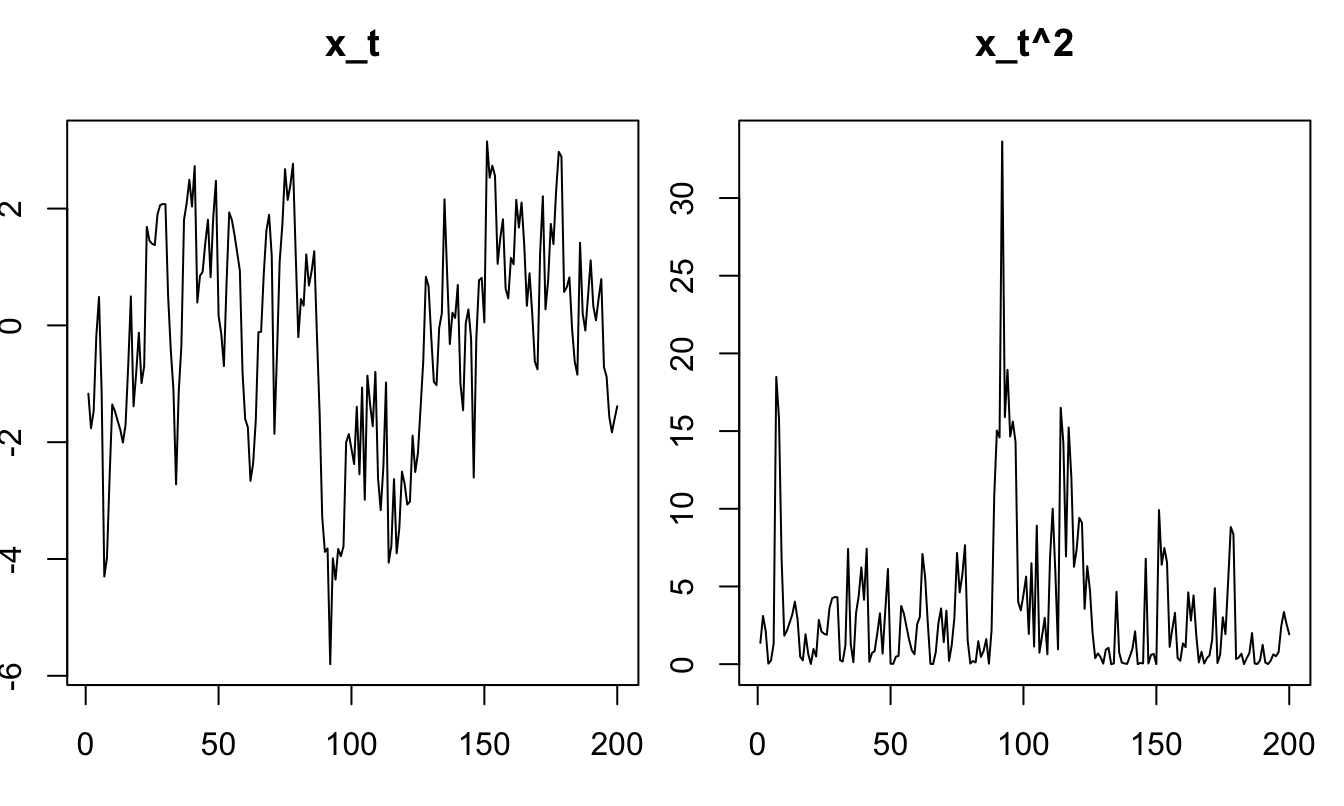
\includegraphics[width=0.95\linewidth]{TSM_files/figure-latex/simQVAR-1} \caption{Simulation of a quadratic processes $x_t$.}\label{fig:simQVAR}
\end{figure}

A term structure illustration is provided in Example \ref{exm:Angetal2011}.
\end{example}

Another example of nonnegative process is that of the auto-regressive Gamma process \citep{Gourieroux_Jasiak_2006} and its extension \citep{zarg_2017}.

\begin{example}[Autoregressive gamma process, ARG(1)]
\protect\hypertarget{exm:ARG1}{}\label{exm:ARG1}

An ARG process is defined as follows:
\[
\frac{w_{t+1}}{\mu} \sim \gamma(\nu+z_t) \quad \mbox{where} \quad z_t \sim \mathcal{P} \left( \frac{\rho w_t}{\mu} \right),
\]
with \(\nu\), \(\mu\), \(\rho > 0\). (Alternatively \(z_t \sim {\mathcal{P}}(\beta w_t)\), with \(\rho = \beta \mu\).)

Proposition \ref{prp:LTARG} shows that we have \(\varphi_t(u) = \exp[a(u)'w_t+b(u)]\) with
\[
\left\{
\begin{array}{cll}
a(u) &=&  \dfrac{\rho u}{1-u \mu}\\
b(u) &=& -\nu  
\log(1-u \mu).
\end{array}
\right.
\]

One can simulate ARG processes by using \href{https://jrenne.shinyapps.io/Affine/}{this web-interface} (select the ``ARG'' panel).

It can be shown that:
\[
\left\{
\begin{array}{cll}
\mathbb{E}(w_{t+1}|\underline{w_t}) &=& \nu \mu + \rho w_t \\
\mathbb{V}ar(w_{t+1}|\underline{w_t}) &=& \nu \mu^2 + 2 \mu \rho w_t.
\end{array}
\right.
\]
and that:
\[
w_{t+1}=\nu\mu+\rho w_t+\varepsilon_{t+1},
\]
where \(\varepsilon_{t+1}\) is a martingale difference \(\Rightarrow\) \(w_{t+1}\) is a weak \(AR(1)\).

\citet{zarg_2017} porpose the extended ARG process and the ARG\(_0\) process. The latter is such that \(\nu = 0\) and \(\beta w_t\) is replaced with \(\alpha + \beta w_t\),\footnote{Zero is an absorbing state for \(w_t\) if \(\alpha = 0\).} i.e.:
\begin{equation}
\frac{w_{t+1}}{\mu} \sim \gamma(z_t),\quad z_t \sim {\mathcal{P}}(\alpha + \beta w_t).\label{eq:ARG0}
\end{equation}
It is easily seen that we then have:
\[
\varphi_t(u) = exp \left[\frac{\beta \mu u}{1-u \mu} w_t + \frac{\alpha \mu u}{1-u \mu}
\right].
\]
The ARG\(_0\) process features a point mass at zero, with conditional probability \(\exp(-\alpha - \beta w_t)\). Note that 0 is absorbing if \(\alpha = 0\).

Figure \ref{fig:simARG0} displays the simulated path of an ARG\(_0\) process (since we set \(\nu\) to zero).

\begin{Shaded}
\begin{Highlighting}[]
\FunctionTok{library}\NormalTok{(TSModels)}
\NormalTok{W }\OtherTok{\textless{}{-}} \FunctionTok{simul.ARG}\NormalTok{(}\DecValTok{300}\NormalTok{,}\AttributeTok{mu=}\NormalTok{.}\DecValTok{5}\NormalTok{,}\AttributeTok{nu=}\DecValTok{0}\NormalTok{,}
               \AttributeTok{rho=}\NormalTok{.}\DecValTok{9}\NormalTok{,}\AttributeTok{alpha=}\NormalTok{.}\DecValTok{1}\NormalTok{) }\CommentTok{\#simul.ARG in package TSModels}
\FunctionTok{plot}\NormalTok{(W,}\AttributeTok{type=}\StringTok{"l"}\NormalTok{)}
\end{Highlighting}
\end{Shaded}

\begin{figure}
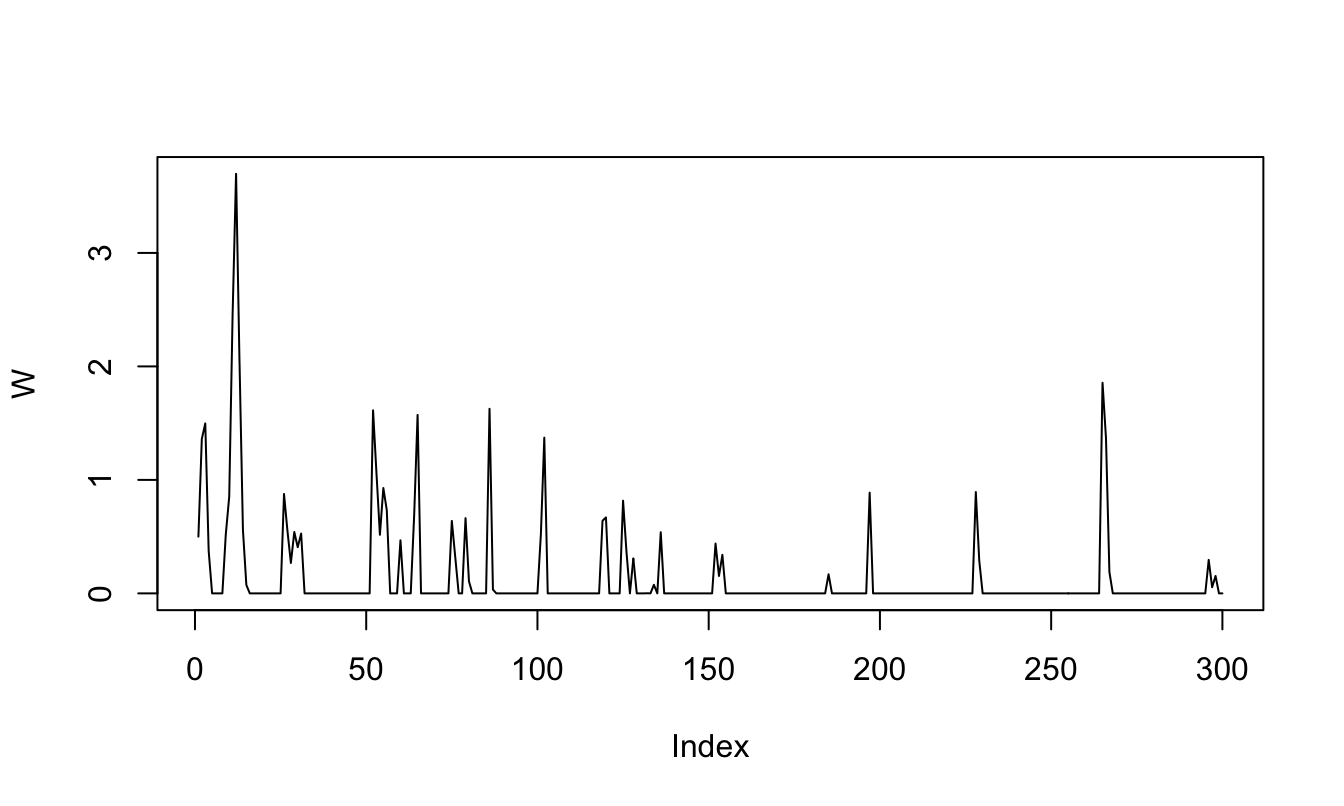
\includegraphics[width=0.95\linewidth]{TSM_files/figure-latex/simARG0-1} \caption{Simulation of an ARG0 processes.}\label{fig:simARG0}
\end{figure}

\end{example}

Certain affine processes are valued in specific sets (e.g., integers). It is the case of compound Poisson proceses:

\begin{example}[Compound Poisson process]
\protect\hypertarget{exm:CompoundPoisson}{}\label{exm:CompoundPoisson}

A compound Poisson process is defined as follows (with \(\gamma > 0\), \(0 < \pi< 1\), and \(\lambda > 0\)):
\[
\frac{w_{t+1}}{\gamma} = z_{t+1} + \varepsilon_{t+1},
\]
where \(z_{t+1}\) and \(\varepsilon_{t+1}\) conditionally independent, and where
\(z_{t+1} \sim {\mathcal B} \left(\frac{w_t}{\gamma},\pi\right)\), with \(\varepsilon_{t+1} \sim {\mathcal P}(\lambda)\).

This process is valued in \(\{j \gamma, j \in \mathbb{N}, \gamma \in \mathbb{R}^+\}\) and we have:
\[
\varphi_t(u) = \exp\left(
\begin{array}{l}
\dfrac{w_t}{\gamma}   \log[\pi
\exp(u\gamma)+1-\pi]-\lambda[1-\exp(u \gamma)]
\end{array}
\right),
\]
i.e., \(\varphi_t(u) = \exp\left(a(u)w_t+b(u)\right)\) with
\[
\left\{
\begin{array}{ccl}
a(u)&=& \frac{1}{\gamma}   \log[\pi   \exp(u
\gamma)+1-\pi],\\
b(u) &=& -\lambda[1-\exp(u \gamma)].
\end{array}
\right.
\]

We also have: \(w_{t+1} = \pi w_t + \lambda \gamma + \eta_{t+1}\), where \(\eta_{t+1}\) is a
martingale difference.

One can simulate such processes by using \href{https://jrenne.shinyapps.io/Affine/}{this web-interface} (select the ``Compound Poisson'' panel). Figure \ref{fig:simCPoisson} makes use of function \texttt{simul.compound.poisson} (in package \texttt{TSModels}) to simulate a compound Poisson process.

\begin{Shaded}
\begin{Highlighting}[]
\FunctionTok{library}\NormalTok{(TSModels)}
\NormalTok{W }\OtherTok{\textless{}{-}} \FunctionTok{simul.compound.poisson}\NormalTok{(}\DecValTok{100}\NormalTok{,}\AttributeTok{Gamma=}\NormalTok{.}\DecValTok{5}\NormalTok{,}\AttributeTok{Pi=}\FloatTok{0.5}\NormalTok{,}\AttributeTok{lambda=}\NormalTok{.}\DecValTok{9}\NormalTok{)}
\FunctionTok{plot}\NormalTok{(W,}\AttributeTok{type=}\StringTok{"l"}\NormalTok{)}
\end{Highlighting}
\end{Shaded}

\begin{figure}
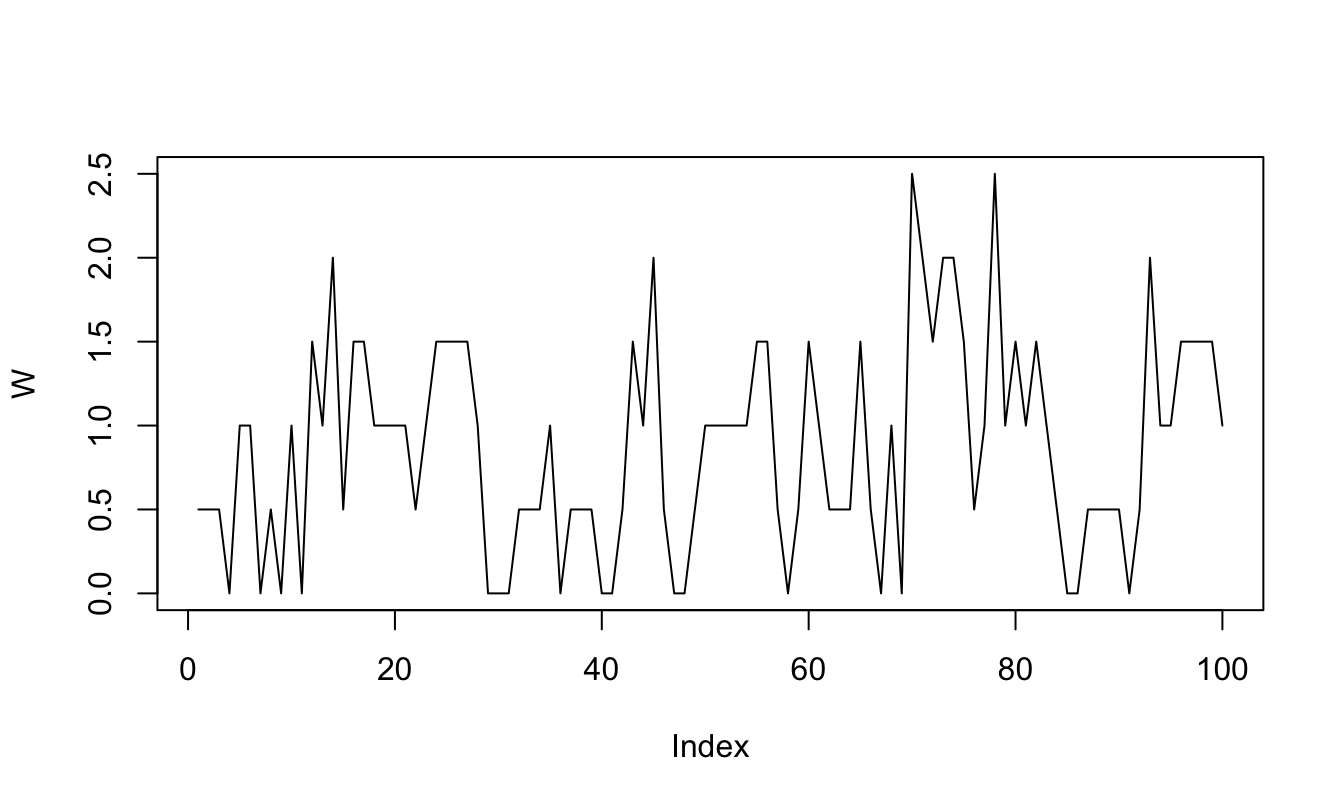
\includegraphics[width=0.95\linewidth]{TSM_files/figure-latex/simCPoisson-1} \caption{Simulation of a Compound Poisson process.}\label{fig:simCPoisson}
\end{figure}

\end{example}

\hypertarget{SubCarp}{%
\subsection{\texorpdfstring{Car processes of order \(p\)}{Car processes of order p}}\label{SubCarp}}

Let us now define Car processes of order \(p\):

\begin{definition}[Affine process of order p]
\protect\hypertarget{def:Carp}{}\label{def:Carp}A multivariate process \(w_{t+1}\) is affine of order \(p\) {[}or \(Car(p)\){]} if there exist functions \(a_1(.),\dots,a_p(.)\), and \(b(.)\) such that:
\[
\varphi_t(u)=\mathbb{E}_t[\exp(u' w_{t+1})]=\exp[a_1(u)'w_t+\dots+a_p(u)'w_{t+1-p}+b(u)].
\]
\end{definition}

It can be seen that if \(w_t\) is \(Car(p)\), then \(W_t = [w_t', w_{t-1}',\dots,w_{t-p+1}']'\) is \(Car(1)\).\footnote{We have:
  \begin{eqnarray*}
  \mathbb{E}_t[\exp(u'W_{t+1})] &=& \mathbb{E}_t[\exp(u'_1 w_{t+1}+u'_2 w_t+\dots+u'_p w_{t-p+2})] \\
  &=& \exp(u'_2 w_t+\dots+u'_p w_{t-p+2})\mathbb{E}_t[\exp(u'_1 w_{t+1})] \\
  &=& \exp(u'_2 w_t+\dots+u'_p w_{t-p+2}+a'_1(u_1)
  w_t  +\dots+a'_p(u_1)w_{t+1-p}+b(u_1)) \\
  &=& \exp[A(u)'W_t+B(u)],
  \end{eqnarray*}
  with \(A(u)' = [u'_2+a'_1(u_1),\dots,u'_p+a'_{p-1}(u_1), a'_p(u_1)]\) and \(B(u) = b(u_1)\).} Therefore, without loss of generality we can assume \(p = 1\).

The standard Car(\(p\)) processes are auto-regressive processes of order \(p\). These processes satisfy the definition of index affine processes:

\begin{definition}[Univariate index affine process of order p]
Let \(\exp[a(u)w_t+b(u)]\) be the conditional Laplace transform of a univariate affine process of order 1, the process \(w_{t+1}\) is an \emph{index-affine} process of order \(p\) if:
\[
\varphi_t(u)=\mathbb{E}_t[\exp(u w_{t+1})]=\exp[a(u)(\beta_1 w_t+\dots+\beta_p
w_{t+1-p})+b(u)].
\]
\end{definition}

Examples \ref{exm:ARp} and \ref{exm:ARGp} are two examples of index affine processes.

\begin{example}[Gaussian AR(p) process]
\protect\hypertarget{exm:ARp}{}\label{exm:ARp}This example extends Example \ref{exm:GAR1}. Consider a Gaussian AR(p) process \(w_t\); that is:
\[
w_{t+1} = \nu + \varphi_1 w_t +\dots+ \varphi_p w_{t+1-p}+\sigma \varepsilon_{t+1},\quad \varepsilon_{t+1} \sim i.i.d. \mathcal{N}(0,1).
\]
We have:
\[
\varphi_t(u) = \exp \left[ u \rho (\beta_1 w_t+\dots+\beta_p w_{t+1-p})+u\nu + u^2  \frac{\sigma^2}{2}\right]
\]
with \(\varphi_i = \rho \beta_i\).
\end{example}

\begin{example}[ARG(p) process (positive)]
\protect\hypertarget{exm:ARGp}{}\label{exm:ARGp}This example extends Example \ref{exm:ARG1}.
An ARG process of order \(p\) is defined as follows:
\[
\frac{w_{t+1}}{\mu} \sim \gamma(\nu+z_t) \quad \mbox{where} \quad z_t \sim \mathcal{P} \left( \beta_1 w_t+\dots+\beta_p w_{t+1-p} \right),
\]
with \(\nu\), \(\mu\), \(\beta_i > 0\). We have:
\[
\varphi_t(u) = \exp\left[\frac{\rho u}{1-u \mu} (\beta_1 w_t+\dots+\beta_p w_{t+1-p})-\nu  \log(1-u\mu)\right],
\]
Process \(w_t\) admits the following AR(\(p\)) representation:
\[
w_{t+1} = \nu\mu + \varphi_1 w_t +\dots+ \varphi_p w_{t+1-p}+\varepsilon_{t+1},
\]
with \(\varphi_i = \beta_i\mu\) and where \(\varepsilon_{t+1}\) is a martingale difference.
\end{example}

\hypertarget{Markov}{%
\section{Markov chains}\label{Markov}}

In this subsection, we show that the family of affine processes includes (some) regime-switching models. We consider a time-homogeneous Markov chain \(z_t\), valued in the set of columns of \(Id_J\), the identity matrix of dimension \(J \times J\). The transition probabilities are denoted by \(\pi(e_i, e_j)\), with \(\pi(e_i, e_j) = \mathbb{P}(z_{t+1}=e_j | z_t=e_i)\). With these notations:
\[
\mathbb{E}[\exp(v'z_{t+1})|z_t=e_i,\underline{z_{t-1}}] = \sum^J_{j=1} \exp(v'e_j)\pi (e_i, e_j).
\]
Hence, we have:
\[
\varphi_t(v) = \exp[a_z(v)'z_t],
\]
with
\[
a_z(v)= \left[ \begin{array}{c} \log \left(\sum^J_{j=1} \exp(v'e_j)  \pi(e_1,e_j)\right)\\
\vdots\\
\log \left(\sum^J_{j=1} \exp(v'e_j)  \pi(e_J,e_j)\right)
\end{array}\right].
\]
This proves that \(z_t\) is an affine process.

One can simulate a two-regime Markov chain by using \href{https://jrenne.shinyapps.io/Affine/}{this web-interface} (select the ``Markov-Switching'' panel).

\hypertarget{WAR}{%
\section{Wishart autoregressive (WAR) processes}\label{WAR}}

WAR are \emph{matrix processes}, valued in the space of \((L \times L)\) symmetric positive
definite matrices.

\begin{definition}[Wishart autoregressive (WAR) processes]
\protect\hypertarget{def:WAR}{}\label{def:WAR}Let \(W_{t+1}\) be a \(WAR_L(K, M, \Omega)\) process. It is defined by:
\begin{eqnarray}
&&\mathbb{E}[\exp   Tr(\Gamma W_{t+1})|\underline{W_t}] \label{eq:Trace}\\
&=& \exp\left\{Tr[M'\Gamma(Id-2\Omega \Gamma)^{-1}M W_t]  -  \frac{K}{2}   \log [det(Id-2\Omega \Gamma)]\right\}, \nonumber
\end{eqnarray}
where \(\Gamma\) is a symmetric matrix,\footnote{Indeed, \(Tr(\Gamma W_{t+1})\) is equal to:
  \(\sum^L_{i=1}(\Gamma W_{t+1})_{ii} = \sum^L_{i=1} \sum^L_{j=1} \gamma_{ij} W_{t+1,ij} = \sum^L_{i=1} \gamma_{ii} W_{t+1,ii} + \sum^L_{i<j} (\gamma_{ij}+\gamma_{ji}) W_{t+1,ij}\).} \(K\) is a positive scalar, \(M\) is a \((L \times L)\) matrix, and \(\Omega\) is a \((L \times L)\) symmetric positive definite matrix.
\end{definition}

If \(K\) is an integer, Proposition \ref{prp:WARAR} (in the appendix) shows that \(W_{t+1}\) can be simulated as:
\begin{eqnarray*}
\left\{
\begin{array}{ccl}
W_{t+1} & =&  \sum^K_{k=1} x_{k,t+1} x'_{k,t+1}\\
x_{k,t+1} &=& M x_{k,t} + \varepsilon_{k,t+1},\quad k \in \{1,\dots,K\},
\end{array}
\right.
\end{eqnarray*}
where \(\varepsilon_{k,t+1} \sim i.i.d. \mathcal{N}(0, \Omega)\) (independent across \(k\)'s).
The proposition also shows that we have:
\[
\mathbb{E}(W_{t+1}|\underline{W_t}) = MW_tM'+K \Omega,
\]
i.e.~\(W_t\) follows a matrix weak AR(1) process.

In particular case, where \(L=1\) (univariate case), we have that:
\begin{eqnarray*}
\mathbb{E}[\exp(u W_{t+1})|\underline{W_t}] = \exp\left[
\frac{u m^2}{1-2\omega u}W_t -
\frac{K}{2}   \log(1-2\omega u)\right].
\end{eqnarray*}
Hence, when \(L=1\), the Wishart process boils down to an \(ARG(1)\) process (Example \ref{exm:ARG1}) with \(\rho = m^2\), \(\mu = 2\omega\), \(\nu = \frac{K}{2}\).

\hypertarget{building}{%
\section{Building affine processes}\label{building}}

\hypertarget{stoch}{%
\subsection{Univariate affine processes with stochastic parameters}\label{stoch}}

Some univariate affine processes can be extended if they satisfy certain conditions. Specifically, consider a univariate affine process whose conditional L.T. is of the form:
\begin{equation}
\mathbb{E}_t   \exp(u y_{t+1}) = \exp[a_0(u)y_t+b_0(u)\delta],\label{eq:extaffine}
\end{equation}
where \(\delta = (\delta_1,\dots,\delta_m)' \in \mathcal{D}\). This process can be generalized by making \(\delta\) stochastic (while staying in the affine family). More precisely assume that:
\[
\mathbb{E}[\exp(u y_{t+1})|\underline{y_t}, \underline{z_{t+1}}] = \exp[a_0(u)y_t+b_0(u)'\Lambda z_{t+1}],
\]
where \(\Lambda\) is a \((m\times k)\) matrix, with \(\Lambda z_{t+1} \in \mathcal{D}\). In this case, if:
\[
\mathbb{E}[\exp(v' z_{t+1})|\underline{y_t}, \underline{z_{t}}] = \exp[a_1(v)'z_t+b_1(v)],
\]
then \(w_{t+1} = (y_{t+1}, z'_{t+1})'\) is affine.\footnote{Indeed, we have:
  \begin{eqnarray*}
  &&\mathbb{E}[\exp(u y_{t+1}+v'z_{t+1})|\underline{y_t}, \underline{z_{t}}] \\
  &=& \mathbb{E}\{\exp(v' z_{t+1})\mathbb{E}[\exp(u y_{t+1})|\underline{y_t},
  \underline{z_{t+1}}]|\underline{y_t}, \underline{z_{t}} \} \\
  &=& \mathbb{E}\{\exp[a_0(u) y_{t}+b_0(u)'\Lambda z_{t+1}+v'z_{t+1}]|\underline{y_t},
  \underline{z_{t}} \} \\
  &=& \exp\{ a_0(u) y_{t}+a_1[\Lambda' b_0(u)+v]'z_t+b_1 [\Lambda' b_0(u)+v]\}.
  \end{eqnarray*}}

\begin{example}[Gaussian AR(p)]
\protect\hypertarget{exm:extendedARp}{}\label{exm:extendedARp}

Using the notation of Example \ref{exm:ARp}, it comes that an AR(p) processes satisfies \eqref{eq:extaffine} with \(b_0(u) = \left(u, \; \frac{u^2}{2}\right)'\) and \(\delta = (\nu,\sigma^2)' \in \mathcal{D}=\mathbb{R} \times \mathbb{R}^+\). In that case, \(\delta\) (the vector of conditional mean and variance) can be replaced by \ldots{}

\begin{itemize}
\tightlist
\item
  \(\left( \begin{array}{l} z_{1,t+1} \\ z_{2,t+1} \end{array} \right)\), where \(z_{1,t+1}\) and \(z_{2,t+1}\) are independent AR(1) (see Example \ref{exm:GAR1}) and ARG(1) (see Example \ref{exm:ARG1}) processes, respectively.
\item
  \(\left( \begin{array}{ll} \lambda'_1 & 0 \\ 0 & \lambda'_2 \end{array} \right)\)\(\left( \begin{array}{l} z_{1,t+1} \\ z_{2,t+1} \end{array} \right)\), where \(z_{1,t+1}\) and \(z_{2,t+1}\) are independent Markov chains.
\item
  \(\left( \begin{array}{l} \lambda'_1 \\ \lambda'_2 \end{array}\right)z_{t+1}\), where \(z_{t+1}\) is a Markov chain.
\end{itemize}

\end{example}

\begin{example}[ARG(p) model]
\protect\hypertarget{exm:ARGp}{}\label{exm:ARGp}\leavevmode

\begin{itemize}
\tightlist
\item
  \(b_0(u)= - \nu \log(1-u\mu)\), \(\delta=\nu\).
\item
  \(\nu\) (\(\ge 0\)) can be specified for instance as a Markov chain or an ARG.
\end{itemize}

\end{example}

\hypertarget{buildingmulti}{%
\subsection{Multivariate affine processes}\label{buildingmulti}}

One can construct multivariate affine processes by employing the so-called recursive approach. Let us illustrate this by considering the bivariate case. (The multivariate generalization is straightforward.) Consider \(w_t = \left(\begin{array}{c} w_{1,t}\\ w_{2,t} \end{array} \right)\),and assume that we have:
\begin{eqnarray*}
&&\mathbb{E}[\exp(u_1 w_{1,t+1}|\underline{w_{1,t}}, \underline{w_{2,t}})]\\
&=& \exp[a_{11}(u_1)w_{1,{\color{red}{t}}}+a_{12}(u_1)w_{2,{\color{red}{t}}}+b_{1}(u_1)],
\end{eqnarray*}
(which defines \(w_{1,t+1}|\underline{w_{1,t}}, \underline{w_{2,t}}\)) and:
\begin{eqnarray*}
&& \mathbb{E}[\exp(u_2 w_{2,t+1}|\underline{w_{1,t+1}}, \underline{w_{2,t}})]\\
&= & \exp[a_0(u_2)w_{1,{\color{red}{t+1}}}+a_{21}(u_2)w_{1,{\color{red}{t}}}+a_{22}(u_2)w_{2,{\color{red}{t}}}+b_2(u_2)]
\end{eqnarray*}
(which defines \(w_{2,t+1}|\underline{w_{1,t+1}}, \underline{w_{2,t}}\)). Then \(w_t\) is an affine process.\footnote{Indeed, we have:
  \begin{eqnarray*}
  && \mathbb{E}[\exp(u_1 w_{1,t+1}+u_2 w_{2,t+1}|\underline{w_{1,t}}, \underline{w_{2,t}})]\\
  &= & \mathbb{E}\{\exp(u_1 w_{1,t+1}) \mathbb{E}[\exp(u_{2}w_{2,t+1})|\underline{w_{1,t+1}}, \underline{w_{2,t}})]|\underline{w_{1,t}}, \underline{w_{2,t}})\} \\
  &= & \mathbb{E}\{\exp[u_1+a_0(u_2)w_{1,t+1}+a_{21}(u_2)w_{1,t} + a_{22}(u_2)w_{2,t}+b_2(u_2)]|\underline{w_{1,t}}, \underline{w_{2,t}})\} \\
  &= & \exp\{a_{11}[u_1+a_0(u_2)]w_{1,t}+a_{12}[u_1+a_0(u_2)]w_{2,t}+b_1[u_1+a_0(u_2)] \\
  &&+  a_{21}(u_2)w_{1,t}+a_{22}(u_2)w_{2,t}+b_2(u_2)\}.
  \end{eqnarray*}}
The joint dynamics of the two components of \(w_t\) can be expressed as:
\begin{eqnarray*}
w_{1,t+1} &=& \alpha_1 + \color{blue}{\alpha_{11}w_{1,t} + \alpha_{12}w_{2,t}} + \varepsilon_{1,t+1} \\
w_{2,t+1} &=& \alpha_2 + \alpha_{0}w_{1,t+1} + \color{blue}{\alpha_{21}w_{1,t} + \alpha _{22} w_{2,t}} + \varepsilon_{2,t+1}.
\end{eqnarray*}
Note that \(\varepsilon_{1,t+1}\) and \(\varepsilon_{2,t+1}\) are non-correlated martingale differences. In the general case, they are conditionally heteroskedastic. What precedes is at play in \(VAR\) model; \citet{zarg_2017} employ this approach to build vector auto-regressive gamma (VARG) processes.

\hypertarget{extending-multivariate-stochastic-processes}{%
\subsection{Extending multivariate stochastic processes}\label{extending-multivariate-stochastic-processes}}

Consider the same framework as in Section \ref{stoch} when \(y_t\) is a \(n\)-dimensional vector. That is, replace \eqref{eq:extaffine} with:
\begin{equation}
\mathbb{E}_t   \exp(u' y_{t+1}) = \exp[a_0(u)'y_t+b_0(u)\delta],\label{eq:Multiextaffine}
\end{equation}
and further assume that \(\delta\) is stochastic and depends on \(z_t\), such that:
\[
\mathbb{E}[\exp(u y_{t+1})|\underline{y_t}, \underline{z_{t+1}}] = \exp[a_0'(u)y_t+b_0(u)\Lambda z_{t+1}],
\]
where \(\Lambda\) is a \((m\times k)\) matrix, with \(\Lambda z_{t+1} \in \mathcal{D}\). In this case, if:
\[
\mathbb{E}[\exp(v' z_{t+1})|\underline{y_t}, \underline{z_{t}}] = \exp[a_1(v)'z_t+b_1(v)],
\]
then \(w_{t+1} = (y_{t+1}, z'_{t+1})'\) is affine.

\begin{example}[Stochastic parameters Gaussian VAR(1)]
\protect\hypertarget{exm:RSVAR}{}\label{exm:RSVAR}

This example extends Example \ref{exm:GVAR1}. Using the same notations as in the latter example \ref{exm:GVAR1}, we have
\[
b_0(u) = \left(u', \frac{1}{2} (u \otimes u)'\right)' \quad \mbox{and} \quad\delta = (\mu', vec(\Sigma)')' \in \mathbb{R}^n \times vec(\mathcal{S}),
\]
where \(\mathcal{S}\) is the set of symmetric positive semi-definite matrices. Vector \(\delta\) can be replaced by \(\left[ \begin{array}{l} z_{1,t+1} \\ z_{2,t+1}\end{array} \right]\), where

\begin{itemize}
\tightlist
\item
  \(z_{1,t+1}\) is, for instance, a Gaussian VAR process.
\item
  \(z_{2,t+1}\) is

  \begin{itemize}
  \tightlist
  \item
    obtained by applying the \(vec\) operator to a Wishart process,
  \item
    replaced by \(\Lambda_2 z_{2,t+1}\), where \(\Lambda_2\) is a \((n^2 \times J)\) matrix whose columns are \(vec(\Sigma_j)\), \(j \in \{1,\dots,J\}\), the \(\Sigma_j\) being \((n \times n)\) positive semi-definite, and \(z_{2,t+1}\) is a selection vector of dimension \(J \times 1\),
  \item
    a standardized \(J\)-dimensional VARG process (multivariate extension of Example \ref{exm:ARG1}).
  \end{itemize}
\end{itemize}

\end{example}

\begin{example}[Regime-switching VAR(1)]
\protect\hypertarget{exm:RSVAR2}{}\label{exm:RSVAR2}

One can also use this approach to construct (affine) regime-switching VAR processes (which is another extension of Example \ref{exm:GVAR1} (see, e.g., \citet{Gourieroux_Monfort_Pegoraro_Renne_2014}). For that, replace \(\delta\) with

\begin{itemize}
\tightlist
\item
  \(\left( \begin{array}{ll} \Lambda_1 & 0 \\ 0 & \Lambda_2 \end{array} \right)\)\(\left( \begin{array}{l} z_{1,t+1} \\ z_{2,t+1} \end{array} \right)\), where \(\Lambda_1\) is a \((n \times J_1)\) matrix and \(z_{1,t+1}\) is a Markov chain valued in the set of selection vectors of size \(J_1\) (see Subsection \ref{Markov}), \(\Lambda_2\) is the same matrix as in Example \ref{exm:RSVAR} and \(z_{2,t+1}\) is a Markov chain valued in the set of selection vectors of size \(J_2\).
\item
  or \(\left( \begin{array}{l} \Lambda_1 \\ \Lambda_2 \end{array}\right)z_{t+1}\), where \(\Lambda_1\) and\(\Lambda_2\) are the same matrices as above with \(J_1=J_2=J\), and \(z_{t+1}\) is a Markov chain valued in the set of selection vectors of size \(J\).
\end{itemize}

\end{example}

\hypertarget{AffineExtended}{%
\subsection{Extended affine processes}\label{AffineExtended}}

Some processes are not affine, but may be sub-components of an affine process. This can be useful to compute their conditional moments and multi-horizon Laplace transform (as one can use the formulas presented above for that, using the enlarged---affine---vector).

Let us formally define an extended affine process:

\begin{definition}[Extended Affine Processes]
\protect\hypertarget{def:ExtAffine}{}\label{def:ExtAffine}A process \(w_{1,t}\) is extended affine if there exists a process \(w_{2,t} = g(\underline{w_{1,t}})\) such that \((w'_{1,t}, w'_{2,t})'\) is affine (of order 1).
\end{definition}

For an extended affine processes, \(\varphi_{1,t}(u) = \mathbb{E}[\exp(u'w_{1,t+1})|\underline{w_{1,t}}]\) can be obtained from:
\begin{eqnarray*}
\varphi_t(u_1, u_2) &=& \mathbb{E}[\exp(u'_1w_{1,t+1}+u'_2 w_{2,t+1)}|\underline{w_{1,t}}, \underline{w_{2,t}}] \\
&=& \exp[a'_1(u_1,u_2)w_{1,t} + a'_2(u_1,u_2)w_{2,t}+b(u_1,u_2)]
\end{eqnarray*}
by:
\[
\varphi_{1,t}(u) = \varphi_t(u, 0) = \exp[a'_1(u,0)w_{1,t}+a'_2(u,0)g(\underline{w_{1,t}}) + b(u, 0)].
\]
In particular \(w_{1,t}\) may be non-Markovian.

Similarly the multi-horizon Laplace transform (see Section \ref{MHLT})
\[
\mathbb{E}[\exp(\gamma'_{1}w_{1,t+1}+\dots+\gamma'_{h}w_{1,t+h})|\underline{w_{1,t}}]
\]
can be obtained from the knowledge of the extended multi-horizon Laplace transform:
\begin{eqnarray*}
&&\mathbb{E}_t[\exp(\{\gamma'_{1,1}w_{1,t+1}+\gamma'_{2,1}w_{2,t+1}\}+\dots+ \{\gamma'_{1,h}w_{1,t+h}+\gamma'_{2,h}w_{2,t+h}\}] \\
&=& \exp[A'_{1,t,h}(\gamma^h_1, \gamma^h_2)w_{1,t}+A'_{2,t,h}(\gamma^h_1, \gamma^h_2)w_{2,t}+B_{t,h}(\gamma^h_1, \gamma^h_2)],
\end{eqnarray*}
(with \(\gamma^h_1 = (\gamma'_{1,1},\dots, \gamma'_{1,h})'\), and \(\gamma^h_2 = (\gamma'_{2,1},\dots, \gamma'_{2,h})'\)). We indeed have:
\begin{eqnarray*}
&& \mathbb{E}[\exp(\gamma'_{1}w_{1,t+1}+\dots+\gamma'_{h}w_{1,t+h})|\underline{w_{1,t}}]\\
&=& \exp[A'_{1,t,h}(\gamma^h,0) w_{1,t} + A'_{2,t,h}(\gamma^h,0)g (\underline{w_{1,t}}) + B_{t,h}(\gamma^h,0)],
\end{eqnarray*}
with \(\gamma^h = (\gamma_1',\dots,\gamma_h')'\).

\begin{example}[Affine process of order p]
\protect\hypertarget{exm:AffProcessOrderp}{}\label{exm:AffProcessOrderp}If \(\{w_{1,t}\}\) is affine or order \(p>1\), then \((w_{1,t},\dots,w_{1,t-p+1})\) is affine of order 1, but \(\{w_{1,t}\}\) is not affine. That is, in that case, \(w_{2,t} = (w'_{1,t-1}, \dots.w'_{1,t-p+1})'\).

This a kind of extreme case since \(w_{2,t}\) belongs to the information at \(t-1\), which implies \(a_2(u_1, u_2) = u_2\).
\end{example}

\begin{example}[Gaussian ARMA process]
\protect\hypertarget{exm:GaussianARMA}{}\label{exm:GaussianARMA}Consider an \(ARMA(1,1)\) process
\[
w_{1,t} - \varphi w_{1,t-1} = \varepsilon_t-\theta \varepsilon_{t-1},
\]
with \(|\varphi | < 1\), \(|\theta| < 1\), and \(\varepsilon_t \sim i.i.d. \mathcal{N}(0, \sigma^2)\).

\(w_{1,t}\) is not Markovian. Now, take \(w_{2,t} = \varepsilon_t = (1-\theta L)^{-1}(1-\varphi L)w_{1,t}\). We have:
\[
\left(
\begin{array}{l}
w_{1,t+1} \\
w_{2,t+1}
\end{array}
\right) =
\left(
\begin{array}{ll}
\varphi & -\theta \\
0 &      0
\end{array}
\right)
\left(
\begin{array}{l}
w_{1,t} \\
w_{2,t}
\end{array}
\right) +
\left(
\begin{array}{l}
1 \\
1
\end{array}
\right) \varepsilon_{t+1}.
\]
Hence \((w_{1,t}, w_{2,t})'\) follows a Gaussian \(VAR(1)\), and, therefore, it is affine of order 1.

This is easily extended to \(ARMA(p,q)\) and \(VARMA(p,q)\) processes.
\end{example}

\begin{example}[GARCH type process]
\protect\hypertarget{exm:GARCH}{}\label{exm:GARCH}Consider process \(w_{1,t}\), defined by:
\[
w_{1,t+1}  = \mu + \varphi w_{1,t} + \sigma_{t+1} \varepsilon_{t+1},
\]
where \(|\varphi| < 1\) and \(\varepsilon_t \sim i.i.d. \mathcal{N}(0,1)\), and
\[
\sigma^2_{t+1} = \omega + \alpha \varepsilon^2_t + \beta \sigma^2_t,
\]
where \(0 < \beta < 1\).

Consider \(w_{2,t} = \sigma^2_{t+1}\) (which is a non-linear function of \(\underline{w_{1,t}}\)). Proposition \ref{prp:GARCH} shows that:
\begin{eqnarray*}
&& \mathbb{E}\left[\exp(u_1 w_{1,t+1} + u_2 w_{2,t+1})|\underline{w_{1,t}}\right] \\
&=& \exp\left[u_1 \mu + u_2 \omega - \frac{1}{2}   \log(1-2 u_2 \alpha) \right. \\
&&\left. +  u_1 \varphi w_{1,t} + (u_2\beta +  \frac{u^2_1}{2(1-2u_2\alpha)}) w_{2,t}\right],
\end{eqnarray*}
which is exponential affine in \((w_{1,t}, w_{2,t})\).
\end{example}

\hypertarget{MHLT}{%
\section{Multi-horizon Laplace transform}\label{MHLT}}

\hypertarget{recursive-computation-and-direct-pricing-implications}{%
\subsection{Recursive computation and direct pricing implications}\label{recursive-computation-and-direct-pricing-implications}}

In this subsection, we show that multi-horizon Laplace transforms of affine processes can be calculated recursively. Various examples will show how this can be exploited to price long-dated financial instruments.

Let us consider a multivariate process \(w_{t}\), affine of order one. (As explained in Subsection \ref{SubCarp}, this includes the case of the order \(p\) case.) For the sake of generality, we consider the case where functions \(a(.)\), \(b(.)\) are possibly deterministic functions of time, denoted in this case \(a_{t+1}(.)\) and \(b_{t+1}(.)\):
\[
\mathbb{E}_t \exp[(u'w_{t+1})] = \exp[a'_{t+1}(u)w_t+b_{t+1}(u)].
\]
The multi-horizon Laplace transform associated with date \(t\) and horizon \(h\) is defined by:
\begin{equation}
\varphi_{t,h}(\gamma_1,\dots,\gamma_h) = \mathbb{E}_t[\exp(\gamma'_1w_{t+1}+\dots+\gamma'_h w_{t+h})].\label{eq:multiLT}
\end{equation}

Lemma \ref{lem:MHLT} (in the appendix) shows that we have:
\[
\varphi_{t,h}(\gamma_1,\dots,\gamma_h) = \exp(A'_{t,h} w_t + B_{t,h}),
\]
where \(A_{t,h} = A^h_{t,h}\) and \(B_{t,h} = B^h_{t,h}\), the \(A^h_{t,i}, B^h_{t,i}\) \(i = 1,\dots,h\), being given recursively by:
\[
\left\{
\begin{array}{ccl}
A^h_{t,i} &=& a_{t+h+1-i}(\gamma_{h+1-i} + A^h_{t,i-1}), \\
B^h_{t,i} &=& b_{t+h+1-i}(\gamma_{h+1-i} + A^h_{t,i-1}) + B^h_{t,i-1}, \\
A^h_{t,0} &=& 0, B^h_{t,0} = 0.
\end{array}
\right.
\]

If the functions \(a_{t}\) and \(b_{t}\) do not depend on \(t\), these recursive formulas do not depend on \(t\), and we get \(\varphi_{t,h}(\gamma_1,\dots,\gamma_h)\), for any \(t\), with only one recursion for each \(h\).

Moreover, if the functions \(a_{t}\) and \(b_{t}\) do not depend on \(t\), and if different sequences \((\gamma^h_1,\dots,\gamma^h_h), h=1,\dots,H\) (say) satisfy \(\gamma^h_{h+1-i} = u_i\), for
\(i=1,\dots,h\), and for any \(h \leq H\), that is if we want to compute (\emph{reverse-order} case):
\begin{equation}
\varphi_{t,h}(u_h,\dots,u_1)=\mathbb{E}_t[\exp(u'_{{\color{red}h}} w_{{\color{red}t+1}}+\dots+u'_{{\color{red}1}} w_{{\color{red}t+h}})],
\quad h=1,\dots,H,\label{eq:LTreverse}
\end{equation}
then Proposition \ref{prp:reverseMLT} (in the appendix) shows that we can compute the \(\varphi_{t,h}(u_h,\dots,u_1)\) for any \(t\) and any \(h \leq H\) with only one recursion. That is \(\varphi_{t,h}(u_h,\dots,u_1)=\exp(A'_hw_t+B_h)\) with:
\begin{equation*}
\left\{
\begin{array}{ccl}
A_{h} &=& a(u_{h} + A_{h-1}), \\
B_{h} &=& b(u_{h} + A_{h-1}) + B_{h-1}, \\
A_{0} &=& 0,\quad  B_{0} = 0.
\end{array}
\right.
\end{equation*}

As mentioned above, what precedes has useful implications to price long-dated financial instruments such as nominal and real bonds (Examples \ref{exm:nominalBth} and \ref{exm:realBth}, respectively), or futures (Example \ref{exm:Futures}).

\begin{example}[Nominal interest rates]
\protect\hypertarget{exm:nominalBth}{}\label{exm:nominalBth}Let \(B_{t,h}\) denote the date-\(t\) price of a nominal zero-coupon bond of maturity \(h\). We have (see \eqref{eq:ihandM} and Subsection \ref{AffineYields}):
\begin{equation}
B_{t,h} = \mathbb{E}^{\mathbb{Q}}_t \exp (-i_{t}-\dots-i_{t+h-1}),\label{eq:stdbond}
\end{equation}
where \(i_{t}\) is the nominal short rate between \(t\) and \(t+1\) (observed at \(t\)), and the associated (continuously-compounded) yield-to-maturity is given by:
\begin{equation}
i_{t,h} = -  \frac{1}{h}   \log   B(t,h), \quad   h=1,\dots,H.
\end{equation}
If \(i_t = \omega'w_t\) (say), then:
\[
B_{t,h} = \exp(-i_{t}) \mathbb{E}^{\mathbb{Q}}_t \exp(-\omega' w_{t+1} - \dots - \omega' w_{t+h-1}).
\]
One can then price this bond by directly employing \eqref{eq:LTreverse}, with \(u_1 = 0\) and \(u_i = - \omega\), \(i = 2,\dots, H\).
The price \(B_{t,h}\) is exponential affine in \(w_t\), the associated yield-to-maturity \(i_{t,h}=-1/h\log B_{t,h}\) is affine in \(w_t\).
\end{example}

\begin{example}[No-arbitrage Nelson-Siegel model]
\protect\hypertarget{exm:CDR2009}{}\label{exm:CDR2009}In this example, we employ the results of Example \ref{exm:nominalBth} in the context described by \citet{Christensen_Diebold_Rudebusch_2009}. Specifically, we consider a three factor model following a Gaussian VAR (see Example \ref{exm:GVAR1}):
\[
w_t = \left[\begin{array}{c}X_{1,t}\\X_{2,t}\\X_{3,t}\end{array}\right] = 
\left[\begin{array}{ccc}
1 & 0 & 0\\
0&1-\lambda&\lambda\\
0&0&1-\lambda\end{array}\right]
\left[\begin{array}{c}X_{1,t-1}\\X_{2,t-1}\\X_{2,t-1}\end{array}\right] +
\left[\begin{array}{ccc}
\sigma_{11} & 0 & 0\\
\sigma_{21}&\sigma_{22}&0\\
\sigma_{31}&\sigma_{32}&\sigma_{33}\end{array}\right]
\left[\begin{array}{c}\varepsilon_{1,t}\\\varepsilon_{2,t}\\\varepsilon_{3,t}\end{array}\right],
\]
where \(\left[\begin{array}{c}\varepsilon_{1,t}\\\varepsilon_{2,t}\\\varepsilon_{3,t}\end{array}\right] \sim \,i.i.d.\, \mathcal{N}(0,Id)\).

The nominal short-term rate is given by \(i_t = X_{1,t}+X_{2,t}\). In that case, we can use the results of Example \ref{exm:nominalBth} with \(\omega = (-1,-1,0)'\). The following lines of code do that:

\begin{Shaded}
\begin{Highlighting}[]
\FunctionTok{library}\NormalTok{(TSModels)}
\NormalTok{lambda }\OtherTok{\textless{}{-}}\NormalTok{ .}\DecValTok{05}
\NormalTok{Phi }\OtherTok{\textless{}{-}} \FunctionTok{diag}\NormalTok{(}\FunctionTok{c}\NormalTok{(}\DecValTok{1}\NormalTok{,}\DecValTok{1}\SpecialCharTok{{-}}\NormalTok{lambda,}\DecValTok{1}\SpecialCharTok{{-}}\NormalTok{lambda));Phi[}\DecValTok{2}\NormalTok{,}\DecValTok{3}\NormalTok{] }\OtherTok{\textless{}{-}}\NormalTok{ lambda}
\NormalTok{Sigma }\OtherTok{\textless{}{-}}\NormalTok{ .}\DecValTok{0005} \SpecialCharTok{*} \FunctionTok{diag}\NormalTok{(}\DecValTok{3}\NormalTok{)}
\NormalTok{psi.parameterization}\OtherTok{=}\FunctionTok{list}\NormalTok{(}\AttributeTok{mu=}\FunctionTok{matrix}\NormalTok{(}\DecValTok{0}\NormalTok{,}\DecValTok{3}\NormalTok{,}\DecValTok{1}\NormalTok{),}\AttributeTok{Phi=}\NormalTok{Phi,}\AttributeTok{Sigma=}\NormalTok{Sigma)}
\NormalTok{u1 }\OtherTok{\textless{}{-}} \FunctionTok{matrix}\NormalTok{(}\DecValTok{0}\NormalTok{,}\DecValTok{3}\NormalTok{,}\DecValTok{1}\NormalTok{)}
\NormalTok{u2 }\OtherTok{\textless{}{-}} \FunctionTok{matrix}\NormalTok{(}\FunctionTok{c}\NormalTok{(}\SpecialCharTok{{-}}\DecValTok{1}\NormalTok{,}\SpecialCharTok{{-}}\DecValTok{1}\NormalTok{,}\DecValTok{0}\NormalTok{),}\AttributeTok{ncol=}\DecValTok{1}\NormalTok{)}
\NormalTok{H }\OtherTok{\textless{}{-}} \DecValTok{20}
\NormalTok{AB }\OtherTok{\textless{}{-}} \FunctionTok{reverse.MHLT}\NormalTok{(psi.GaussianVAR,}\AttributeTok{u1 =}\NormalTok{ u1,}\AttributeTok{u2 =}\NormalTok{ u2,}\AttributeTok{H =}\NormalTok{ H,}
                   \AttributeTok{psi.parameterization =}\NormalTok{ psi.parameterization)}
\NormalTok{AB}\SpecialCharTok{$}\NormalTok{A[}\DecValTok{1}\SpecialCharTok{:}\DecValTok{2}\NormalTok{,,] }\OtherTok{\textless{}{-}}\NormalTok{ AB}\SpecialCharTok{$}\NormalTok{A[}\DecValTok{1}\SpecialCharTok{:}\DecValTok{2}\NormalTok{,,] }\SpecialCharTok{{-}} \DecValTok{1} \CommentTok{\# add terms for exp({-}i\_t)}
\NormalTok{a.yield }\OtherTok{\textless{}{-}} \SpecialCharTok{{-}}\NormalTok{ AB}\SpecialCharTok{$}\NormalTok{A }\SpecialCharTok{/} \FunctionTok{array}\NormalTok{((}\DecValTok{1}\SpecialCharTok{:}\NormalTok{H) }\SpecialCharTok{\%x\%} \FunctionTok{rep}\NormalTok{(}\DecValTok{1}\NormalTok{,}\DecValTok{3}\NormalTok{),}\FunctionTok{c}\NormalTok{(}\DecValTok{3}\NormalTok{,}\DecValTok{1}\NormalTok{,H))}
\NormalTok{b.yield }\OtherTok{\textless{}{-}} \SpecialCharTok{{-}}\NormalTok{ AB}\SpecialCharTok{$}\NormalTok{B }\SpecialCharTok{/} \FunctionTok{array}\NormalTok{((}\DecValTok{1}\SpecialCharTok{:}\NormalTok{H) }\SpecialCharTok{\%x\%} \FunctionTok{rep}\NormalTok{(}\DecValTok{1}\NormalTok{,}\DecValTok{3}\NormalTok{),}\FunctionTok{c}\NormalTok{(}\DecValTok{1}\NormalTok{,}\DecValTok{1}\NormalTok{,H))}
\FunctionTok{plot}\NormalTok{(a.yield[}\DecValTok{1}\NormalTok{,,],}\AttributeTok{type=}\StringTok{"l"}\NormalTok{,}\AttributeTok{lwd=}\DecValTok{2}\NormalTok{,}\AttributeTok{ylim=}\FunctionTok{c}\NormalTok{(}\DecValTok{0}\NormalTok{,}\DecValTok{1}\NormalTok{),}
     \AttributeTok{xlab=}\StringTok{"Maturity"}\NormalTok{,}\AttributeTok{ylab=}\StringTok{"Factor loadings"}\NormalTok{)}
\FunctionTok{lines}\NormalTok{(a.yield[}\DecValTok{2}\NormalTok{,,],}\AttributeTok{col=}\StringTok{"red"}\NormalTok{,}\AttributeTok{lwd=}\DecValTok{2}\NormalTok{,}\AttributeTok{lty=}\DecValTok{2}\NormalTok{)}
\FunctionTok{lines}\NormalTok{(a.yield[}\DecValTok{3}\NormalTok{,,],}\AttributeTok{col=}\StringTok{"blue"}\NormalTok{,}\AttributeTok{lwd=}\DecValTok{2}\NormalTok{,}\AttributeTok{lty=}\DecValTok{3}\NormalTok{)}
\end{Highlighting}
\end{Shaded}

\begin{figure}
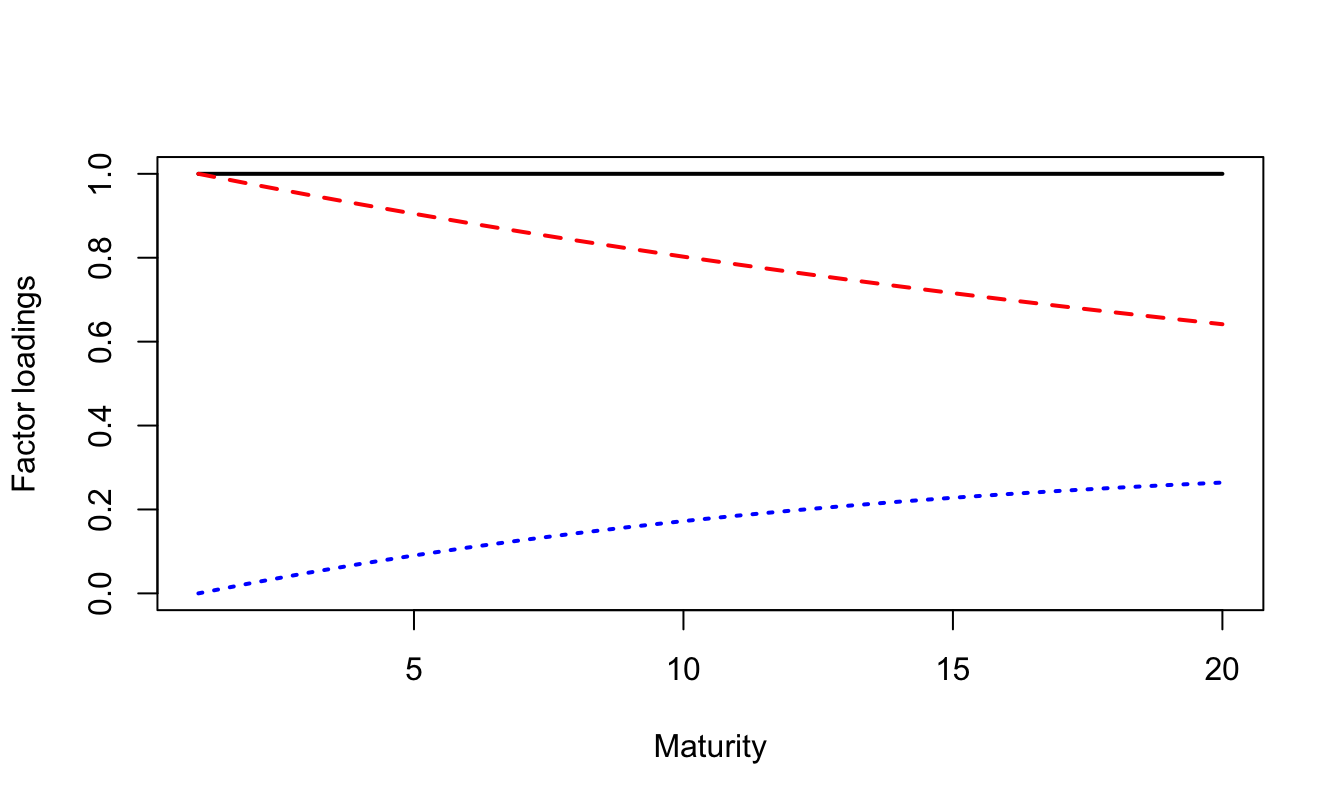
\includegraphics[width=0.95\linewidth]{TSM_files/figure-latex/CDR-1} \caption{Factor loadings in the context of a no-arbitrage nelson-Siegel model (Christensen, Diebold and Rudebusch, 2009). The first factor (black solid line) is a level factor. The second and third factors (red dashed line and blue dotted line, respectively) are slope factors.}\label{fig:CDR}
\end{figure}

\citet{Christensen_Diebold_Rudebusch_2009} show that such specifications allow to approximate the widely-used \citet{Nelson_Siegel_1987} yield curve specification.\footnote{In the context of the Nelson-Siegel model, the zero-coupon yield of maturity \(h\) is given by \(\beta_0 + \beta_1\left(\frac{1 - \exp(-\lambda h)}{\lambda h}\right)+\beta_2\left(\frac{1 - \exp(-\lambda h)}{\lambda h}-\exp(-\lambda h)\right)\), where \(\beta_0\), \(\beta_1\), \(\beta_2\), and \(\lambda\) are parameters.}
\end{example}

In the previous example, note the use of function \texttt{reverse.MHLT} (in package \texttt{TSModels}), that notably takes a L.T. as an argument (\texttt{psi}). In the previous example, we consider a Gaussian VAR, and we therefore assign \texttt{psi.GaussianVAR} to \texttt{psi}. We then need to provide function \texttt{reverse.MHLT} with the arguments of the \texttt{psi} function. These arguments are provided in the form of a list (input \texttt{psi.parameterization}).

\begin{example}[Real interest rates]
\protect\hypertarget{exm:realBth}{}\label{exm:realBth}Denote by \(q_t\) the price index on date \(t\) and by \(\pi_{t+1} = \log \dfrac{q_{t+1}}{q_t}\) the inflation rate on date \(t+1\). The real rate of maturity \(h\) is given by (see Subsection \ref{AffineYields}):
\begin{eqnarray*}
r_{t,h} & =& -   \frac{1}{h}   \log   \mathcal{B}_{t,h}, \quad h=1,\dots,H \\    \\
\mathcal{B}_{t,h} & =&  \mathbb{E}^{\mathbb{Q}}_t   \exp(-r_{t}-\dots-r_{t+h-1} + \pi_{t+1}+\dots+\pi_{t+h}),  \\      \\
& =& \exp(-r_{t}) \times \\
&& \mathbb{E}^{\mathbb{Q}}_t \exp(-r_{t+1}-\dots-r_{t+h-1}+\pi_{t+1}+\dots+\pi_{t+h}),
\end{eqnarray*}
where \(r_t\) is the short-term real rate and \(\mathcal{B}_{t,h}\) is the price of a real zero-coupon bond of maturity \(h\) (which is also a inflation-indexed zero-coupon bond).
If \(r_t = \omega'w_t\) and \(\pi_t = \bar\omega'w_t\), then \(\mathcal{B}_{t,h}\) is given by:
\begin{eqnarray*}
\exp(-r_{t}) \mathbb{E}^{\mathbb{Q}}_t \exp[(\bar\omega-\omega)'w_{t+1}+\dots+(\bar\omega-\omega)'w_{t+h-1}+\bar\omega'
w_{t+h}]
\end{eqnarray*}
One can then price this bond by directly employing \eqref{eq:LTreverse}, with \(u_1 = \bar\omega\) and \(u_i = \bar\omega-\omega\), \(i = 2,\dots, H\).
\end{example}

\begin{example}[Futures]
\protect\hypertarget{exm:Futures}{}\label{exm:Futures}

Denote by \(F(t,h)\) the date-\(t\) price of a future of maturity \(h\) (see Subsection \ref{FCFPFutures}). That is \(F(t,h) = \mathbb{E}^{\mathbb{Q}}_t (S_{t+h})\), \(h=1,\dots,H\), where \(S_t\) is the date-\(t\) price of the underlying asset.

\begin{itemize}
\item
  If \(w_t = (\log S_t, x'_t)'\) then \(F(t,h) = \mathbb{E}^{\mathbb{Q}}_t \exp(e'_1 w_{t+h})\). This can be calculated by using \eqref{eq:LTreverse} with \(u_1 = e_1\), and \(u_i = 0\), for \(i=2,\dots,H\).
\item
  If \(w_t = (y_t, x'_t)'\) with \(y_t = \log\frac{S_t}{S_{t-1}}\), then \(F(t,h) = S_t \mathbb{E}^{\mathbb{Q}}_t \exp(e'_1 w_{t+1}+\dots+e'_1 w_{t+h})\). This can be calculated by using \eqref{eq:LTreverse} with \(u_i = e'_1\), \(i=1,\dots,H\).
\end{itemize}

\end{example}

\hypertarget{ExponentialPayoff}{%
\subsection{Exponential payoff}\label{ExponentialPayoff}}

Consider an asset providing the payoff \(\exp(\nu' w_{t+h})\) on date \(t+h\). Its price is given by:
\[
P(t,h;\nu) = \mathbb{E}^{\mathbb{Q}}_t[\exp(-i_{t}-\dots-i_{t+h-1}) \exp(\nu' w_{t+h})].
\]
If \(i_t = \omega'w_t\), we have:
\[
P(t,h;\nu) = \exp(-r_{t})\mathbb{E}^{\mathbb{Q}}_t \left(\exp[-\omega' w_{t+1}-\dots-\omega' w_{t+h-1}+ \nu' w_{t+h}]\right),
\]
which can be calculated by \eqref{eq:LTreverse}, with \(u_1 = \nu\) and \(u_i = -\omega\) for \(i = 2,\dots,H\).

What precedes can be extended to the case where the payoff (settled on date \(t+h\)) is of the form:
\[
(\nu_1'w_{t+h}) \exp(\nu_2' w_{t+h}).
\]
Indeed, we have
\[
\left[\frac{\partial \exp[(s \nu_1+ \nu_2)'w_{t+h}]}{\partial s}\right]_{s=0} = (\nu_1'w_{t+h}) \exp(\nu_2' w_{t+h}).
\]
Therefore:
\begin{eqnarray}
&&\mathbb{E}_t^{\mathbb{Q}}[\exp(-i_t - \dots - i_{t+h-1})(\nu_1'w_{t+h}) \exp(\nu_2' w_{t+h})] \nonumber\\
&=& \left[
\frac{\partial P(t,h;s \nu_1 + \nu_2)}{\partial s}
\right]_{s=0}.\label{eq:Affineexppayoff}
\end{eqnarray}
This method is easily extended to price payoffs of the form \((\nu_1'w_{t+h})^k \exp(\nu_2' w_{t+h})\), with \(k \in \mathbb{N}\).

\hypertarget{var-representation-and-conditional-moments}{%
\section{VAR representation and conditional moments}\label{var-representation-and-conditional-moments}}

An important property of affine processes is that their dynamics can be written as a vector-autoregressive process. This is useful to compute conditional moments of the process.

\begin{proposition}[VAR representation of an affine process' dynamics]
\protect\hypertarget{prp:affineVAR}{}\label{prp:affineVAR}If \(w_t\) is the affine process whose Laplace transform is defined in Def. \ref{def:Car1}, then its dynamics admits the following vectorial autoregressive representation:
\begin{equation}
w_{t+1} = \mu + \Phi w_{t} + \Sigma^{\frac{1}{2}}(w_t) \varepsilon_{t+1},\label{eq:VARw}
\end{equation}
where \(\varepsilon_{t+1}\) is a difference of martingale sequence whose conditional covariance matrix is the identity matrix and where \(\mu\), \(\Phi\) and \(\Sigma(w_t) = \Sigma^{\frac{1}{2}}(w_t){\Sigma^{\frac{1}{2}}(w_t)}'\) satisfy:
\begin{equation}
\mu =  \left[\frac{\partial }{\partial u}b(u)\right]_{u=0}, \quad \Phi= \left[\frac{\partial }{\partial u}a(u)'\right]_{u=0}\label{eq:MUPHI}
\end{equation}
\begin{equation}
\Sigma(w_t) =  \left[\frac{\partial }{\partial u\partial u'}b(u)\right]_{u=0} + \left[\frac{\partial }{\partial u\partial u'}a(u)'w_t\right]_{u=0}.\label{eq:SigmaWt}
\end{equation}
\end{proposition}

\begin{proof}
When \(w_t\) is affine, its (conditional) cumulant generating function is of the form \(\psi(u)=a(u)'w_t+b(u)\). The result directly follows from the formulas given in Section \ref{AffineLaplace}.
\end{proof}

Proposition \ref{prp:condvarAffine} (in the appendix) further shows that the conditional means and variances of \(w_t\) are given by:
\begin{eqnarray}
\mathbb{E}_t(w_{t+h}) &=& (I - \Phi)^{-1}(I - \Phi^h)\mu + \Phi^h w_t \label{eq:condmean}\\
\mathbb{V}ar_t(w_{t+h}) &=& \Sigma(\mathbb{E}_t(w_{t+h-1}))+\Phi \Sigma(\mathbb{E}_t(w_{t+h-2}))\Phi' + \nonumber \\
&& \dots + \Phi^{h-1} \Sigma(w_{t}){\Phi^{h-1}}'. \label{eq:condvar}
\end{eqnarray}
Eq. \eqref{eq:condvar} notably implies that \(\mathbb{V}ar_t(w_{t+h})\) is an affine function of \(w_t\). Indeed \(\Sigma(.)\) is an affine function, and the conditional expectations \(\mathbb{E}_t(w_{t+h})\) are affine in \(w_t\), as shown by \eqref{eq:condmean}.

The unconditional means and variances are given by:
\begin{equation}
\left\{
\begin{array}{ccl}
\mathbb{E}(w_t) &=& (I - \Phi)^{-1}\mu\\
vec[\mathbb{V}ar(w_t)] &=& (I_{n^2} - \Phi \otimes \Phi)^{-1} vec\left(\Sigma[(I - \Phi)^{-1}\mu]\right).
\end{array}
\right.\label{eq:uncondmeanvar}
\end{equation}

\hypertarget{TransfAna}{%
\section{Truncated Laplace transforms of affine processes}\label{TransfAna}}

In this section, we show how one can employ Fourier transforms to compute truncated conditional moments of affine processes. For that, let us introduce the following notation:
\[
w_{t+1,T} = (w'_{t+1}, w'_{t+2},\dots, w'_T)'
\]
with \(w_t\) affine \(n\)-dimensional process.

We want to compute:
\[
\tilde{\varphi}_t(u ; v, \gamma) = \mathbb{E}_t[\exp(u'w_{t+1,T})\textbf{1}_{\{v'w_{t+1,T}<\gamma\}}].
\]

Consider the complex untruncated conditional Laplace transform:
\[
\varphi_t(z) = \mathbb{E}_t[\exp(z'w_{t+1,T})],\quad  z \in \mathbb{C}^{nT},
\]
computed using the same recursive algorithm as in the real case (see Section \ref{MHLT}).

\citet{Duffie_Pan_Singleton_2000} have shown that we have (see also Proposition \ref{prp:Fourier} in the appendix):
\begin{equation}
\tilde{\varphi}_t(u ; v, \gamma) =  \frac{\varphi_t(u)}{2} - \frac{1}{\pi}
\int^\infty_0 \frac{Im[\varphi_t(u+ivx) \exp(-i\gamma x)]}{x} dx.\label{eq:DPS}
\end{equation}
where \(Im\) means imaginary part.

Note that the integral in \eqref{eq:DPS} is one dimensional (whatever the dimension of \(w_t\)). As shown in the following example, this can be exploited to price options.

\begin{example}[Option pricing]
\protect\hypertarget{exm:OptionPricing}{}\label{exm:OptionPricing}Pricing calls and puts amounts to conditional expectations of the type (with \(k > 0\)):
\begin{eqnarray*}
&& \mathbb{E}_t\left([\exp(u'_1 w_{t+1,T})-k   \exp(u'_2 w_{t+1,T})]^+\right) \\
&= &  \mathbb{E}_t\left([\exp(u'_1 w_{t+1,T})-k   \exp(u'_2 w_{t+1,T})]\textbf{1}_{\{[\exp(u_1-u_2)'w_{t+1,T}] > k \}}\right) \\
&= & \tilde{\varphi}_t(u_1 ; u_2-u_1, - \log   k) - k \tilde{\varphi}_t(u_2 ; u_2-u_1, - \log   k).
\end{eqnarray*}
\end{example}

\begin{example}[Exogenous short rate]
\protect\hypertarget{exm:ExogSTR}{}\label{exm:ExogSTR}Consider an asset whose date-\(t\) price is \(p_t\). Denote its geometric asset return by \(y_t\), i.e., \(y_t = \log(p_t/p_{t-1})\). Consider an option written on this asset, with a strike equal \(k p_t\).

If interest rates are deterministic, the option price, for a maturity \(h\), is given by:
\[
p_t   \exp(-i_{t}-\dots-i_{t+h-1}) \mathbb{E}^{\mathbb{Q}}_t[\exp   u'_1 w_{t+1, t+h} - k]^+
\]
with \(u_1 = e \otimes e_1\), where \(e\) is the \(h\)-dimensional vector with components equal to 1, and \(e_1\) is the \(n\)-vector selecting the 1st component (\(y_t\) being the 1st component of \(w_t\), say).
\end{example}

\begin{example}[Endogenous short rate]
\protect\hypertarget{exm:EndogSTR}{}\label{exm:EndogSTR}Consider the same context as in Example \ref{exm:ExogSTR}, but with a stochastic (endogenous) short-term rate. For instance, assume that \(i_{t+1} = \omega_0 + \omega'_1 w_t\). The option price then is:
\begin{eqnarray*}
&& p_t \mathbb{E}^{\mathbb{Q}}_t  \left[ \exp(-\omega_0 - \omega'_1 w_t-\dots- \omega_0 - \omega'_1 w_{t+h-1}) [\exp(u'_1 w_{t+1,t+h})-k]^+ \right]\\
&= & p_t   \exp(-h \omega_0 - \omega'_1 w_t)\mathbb{E}^{\mathbb{Q}}_t\left(\left[\exp(\tilde{u}'_1w_{t+1,t+h})-k   \exp(u_2 w_{t+1, t+h})\right]^+\right),
\end{eqnarray*}
with \(\tilde{u}'_1 = u_1 + u_2\), {[}\(u_1 = e \otimes e_1\) as before{]}, and \(u_2 = (-\omega'_1,\dots, -\omega'_1, 0)'\).
\end{example}

\begin{example}[Numerical example: Conditional cumulated distribution function (c.d.f.)]
\protect\hypertarget{exm:truncatedR}{}\label{exm:truncatedR}

Let us use the model used in Example \ref{exm:CDR2009}. Suppose we want to compute the conditional distribution of the average interest rate over the next \(H\) periods, i.e., \(\frac{1}{H}(i_{t+1}+\dots+i_{t+H})\). Hence, we want to compute \(\mathbb{E}_t[\textbf{1}_{\{v'w_{t+1,T}<\gamma\}}]\) with \(v'w_{t+1,T}=\frac{1}{H}(i_{t+1}+\dots+i_{t+H})\).

\begin{Shaded}
\begin{Highlighting}[]
\NormalTok{H  }\OtherTok{\textless{}{-}} \DecValTok{10}
\NormalTok{X  }\OtherTok{\textless{}{-}} \FunctionTok{matrix}\NormalTok{(}\FunctionTok{c}\NormalTok{(}\FloatTok{0.01}\NormalTok{,.}\DecValTok{02}\NormalTok{,}\DecValTok{0}\NormalTok{),}\DecValTok{3}\NormalTok{,}\DecValTok{1}\NormalTok{)}
\NormalTok{x  }\OtherTok{\textless{}{-}} \FunctionTok{exp}\NormalTok{(}\FunctionTok{seq}\NormalTok{(}\SpecialCharTok{{-}}\DecValTok{10}\NormalTok{,}\DecValTok{10}\NormalTok{,}\AttributeTok{length.out=}\DecValTok{1000}\NormalTok{))}
\NormalTok{u1 }\OtherTok{\textless{}{-}} \FunctionTok{matrix}\NormalTok{(}\FunctionTok{c}\NormalTok{(}\DecValTok{1}\SpecialCharTok{/}\NormalTok{H,}\DecValTok{1}\SpecialCharTok{/}\NormalTok{H,}\DecValTok{0}\NormalTok{),}\DecValTok{3}\NormalTok{,}\DecValTok{1}\NormalTok{) }\SpecialCharTok{\%*\%} \FunctionTok{matrix}\NormalTok{(1i}\SpecialCharTok{*}\NormalTok{x,}\AttributeTok{nrow=}\DecValTok{1}\NormalTok{);u2 }\OtherTok{\textless{}{-}}\NormalTok{ u1}
\NormalTok{AB }\OtherTok{\textless{}{-}} \FunctionTok{reverse.MHLT}\NormalTok{(psi.GaussianVAR,}\AttributeTok{u1 =}\NormalTok{ u1,}\AttributeTok{u2 =}\NormalTok{ u2,}\AttributeTok{H =}\NormalTok{ H,}
                   \AttributeTok{psi.parameterization =}\NormalTok{ psi.parameterization)}
\NormalTok{s1 }\OtherTok{\textless{}{-}} \FunctionTok{matrix}\NormalTok{(}\FunctionTok{exp}\NormalTok{(}\FunctionTok{t}\NormalTok{(X) }\SpecialCharTok{\%*\%}\NormalTok{ AB}\SpecialCharTok{$}\NormalTok{A[,,H] }\SpecialCharTok{+}\NormalTok{ AB}\SpecialCharTok{$}\NormalTok{B[,,H]),}\AttributeTok{ncol=}\DecValTok{1}\NormalTok{)}
\NormalTok{dx }\OtherTok{\textless{}{-}} \FunctionTok{matrix}\NormalTok{(x}\SpecialCharTok{{-}}\FunctionTok{c}\NormalTok{(}\DecValTok{0}\NormalTok{,x[}\DecValTok{1}\SpecialCharTok{:}\FunctionTok{length}\NormalTok{(x)}\SpecialCharTok{{-}}\DecValTok{1}\NormalTok{]),}\FunctionTok{length}\NormalTok{(x),}\DecValTok{1}\NormalTok{)}
\NormalTok{gamma }\OtherTok{\textless{}{-}} \FunctionTok{seq}\NormalTok{(}\SpecialCharTok{{-}}\NormalTok{.}\DecValTok{2}\NormalTok{,.}\DecValTok{3}\NormalTok{,}\AttributeTok{length.out=}\DecValTok{1000}\NormalTok{)}
\NormalTok{fx }\OtherTok{\textless{}{-}} \FunctionTok{outer}\NormalTok{(x,gamma,}\ControlFlowTok{function}\NormalTok{(r,c)\{}\FunctionTok{Im}\NormalTok{(s1[,}\DecValTok{1}\NormalTok{]}\SpecialCharTok{*}
                                       \FunctionTok{exp}\NormalTok{(}\SpecialCharTok{{-}}\NormalTok{1i}\SpecialCharTok{*}\NormalTok{r}\SpecialCharTok{*}\NormalTok{c))}\SpecialCharTok{/}\NormalTok{r\})}\SpecialCharTok{*}\NormalTok{dx[,}\DecValTok{1}\NormalTok{]}
\NormalTok{f  }\OtherTok{\textless{}{-}} \DecValTok{1}\SpecialCharTok{/}\DecValTok{2} \SpecialCharTok{{-}} \DecValTok{1}\SpecialCharTok{/}\NormalTok{pi }\SpecialCharTok{*} \FunctionTok{apply}\NormalTok{(fx,}\DecValTok{2}\NormalTok{,sum)}
\FunctionTok{plot}\NormalTok{(gamma,f,}\AttributeTok{type=}\StringTok{"l"}\NormalTok{,}\AttributeTok{xlab=}\StringTok{""}\NormalTok{,}\AttributeTok{lwd=}\DecValTok{2}\NormalTok{)}
\end{Highlighting}
\end{Shaded}

\begin{figure}
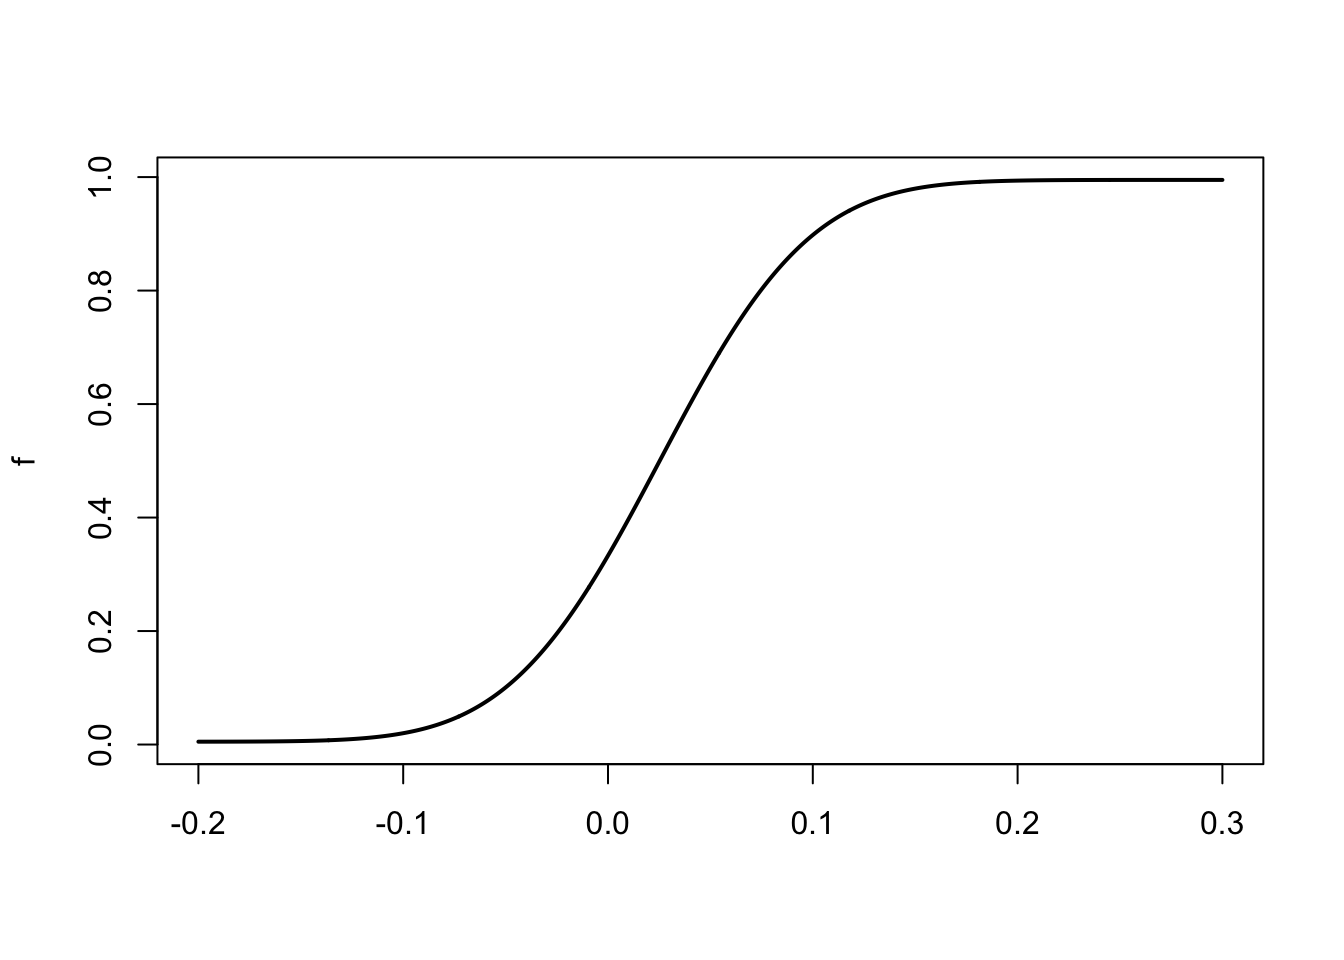
\includegraphics{TSM_files/figure-latex/truncatedRR-1} \caption{Conditional cumulated distribution function (c.d.f.) of $\frac{1}{H}(i_{t+1}+\dots+i_{t+H})$.}\label{fig:truncatedRR}
\end{figure}

\end{example}

\hypertarget{appendices}{%
\section{Appendices}\label{appendices}}

\begin{lemma}
\protect\hypertarget{lem:integralQuadratic}{}\label{lem:integralQuadratic}If \(\mu \in \mathbb{R}^L\) and \(Q\) is a \((L \times L)\) matrix symmetric positive definite, then:
\[
\int_{\mathbb{R}^{L}} \exp(-u'Q u + \mu'u)du =
\frac{\pi^{L/2}}{(det   Q)^{1/2}} \exp \left(
\begin{array}{l}  \frac{1}{4} \mu'Q^{-1}\mu \end{array} \right).
\]
\end{lemma}

\begin{proof}
The integral is:
\begin{eqnarray*}
&& \int_{\mathbb{R}^{L}} exp \left[ \begin{array}{l} - (u -
\frac{1}{2}  Q^{-1} \mu)'  Q (u -
\frac{1}{2} Q^{-1} \mu)'
\end{array}
\right] exp\left(
\begin{array}{l}  \frac{1}{4} \mu'Q^{-1}\mu \end{array}
\right)du \\
&=&  \frac{\pi^{L/2}}{(det Q)^{1/2}} exp\left(
\begin{array}{l}  \frac{1}{4} \mu'Q^{-1}\mu \end{array}
\right)
\end{eqnarray*}
{[}using the formula for the unit mass of \(\mathcal{N}( 0.5Q^{-1}\mu,(2Q)^{-1})\){]}.
\end{proof}

\begin{lemma}
\protect\hypertarget{lem:Quadr}{}\label{lem:Quadr}If \(\varepsilon_{t+1} \sim \mathcal{N}(0,Id)\), we have
\[
\mathbb{E}_t \left(\exp[\lambda'\varepsilon_{t+1}+\varepsilon'_{t+1} V \varepsilon_{t+1}]\right) =  \frac{1}{[\det(I-2V)]^{1/2}} \exp\left[
\frac{1}{2} \lambda'(I-2V)^{-1}\lambda
\right].
\]
\end{lemma}

\begin{proof}
We have
\[
\mathbb{E}_t   \exp(\lambda'\varepsilon_{t+1}+\varepsilon'_{t+1}V\varepsilon_{t+1})
=  \frac{1}{(2\pi)^{n/2}}  \int_{\mathbb{R}^{n}} \exp\left[
\begin{array}{l}
-u'\left(
\begin{array}{l}
\frac{1}{2} I-V
\end{array}
\right)u+\lambda'u
\end{array}
\right]du
\]
From Lemma \ref{lem:integralQuadratic}, if \(u\in\mathbb{R}^n\), then
\[
\int_{\mathbb{R}^{n}} \exp(-u' Q u+\mu'u) du =
\frac{\pi^{n/2}}{(\det Q)^{1/2}} \exp\left(
\begin{array}{l}
\frac{1}{4} \mu'Q^{-1}\mu
\end{array}
\right).
\]
Therefore:
\[
\begin{array}{l}
\mathbb{E}_t   \exp(\lambda'\varepsilon_{t+1}+\varepsilon'_{t+1}V\varepsilon_{t+1}) \\
=  \frac{1}{2^{n/2}
\left[
\begin{array}{l}
\det \left(
\begin{array}{l}
\frac{1}{2} I-V
\end{array}
\right)
\end{array}
\right]^{1/2}
}
\exp\left[
\begin{array}{l}
\frac{1}{4}  \lambda'\left(
\begin{array}{l}
\frac{1}{2} I-V
\end{array}
\right)^{-1}\lambda
\end{array}
\right].
\end{array}
\]
\end{proof}

\begin{proposition}[Quadratic Gaussian process]
\protect\hypertarget{prp:QGVAR1}{}\label{prp:QGVAR1}Consider vector \(w_t = (x'_t,vec(x_t x_t')')'\), where \(x_t\) is a \(n\)-dimensional vector following a Gaussian VAR(1), i.e.
\[
x_{t+1}|\underline{w_t} \sim \mathcal{N}(\mu+\Phi x_t, \Sigma).
\]
If \(u = (v,V)\) where \(v \in \mathbb{R}^n\) and \(V\) a square symmetric matrix of size \(n\), we have:
\begin{eqnarray*}
\varphi_t(u) &=& \mathbb{E}_t\big\{\exp\big[(v',vec(V)')\times w_{t+1}\big]\big\} \\
& =& \exp \left\{a_1(v,V)'x_t +vec(a_2(v,V))' vec(x_t'x_t) + b(v,V) \right\},
\end{eqnarray*}
where:
\begin{eqnarray*}
a_2(u) & = & \Phi'V (I_n - 2\Sigma V)^{-1} \Phi \nonumber \\
a_1(u) & = & \Phi'\left[(I_n-2V\Sigma)^{-1}(v+2V\mu)\right] \nonumber \\
b(u) & = & u'(I_n - 2 \Sigma V)^{-1}\left(\mu + \frac{1}{2} \Sigma v\right) +\\
&& \mu'V(I_n - 2 \Sigma V)^{-1}\mu - \frac{1}{2}\log\big|I_n - 2\Sigma V\big|.\label{eq:laplaceZ}
\end{eqnarray*}
\end{proposition}

\begin{proof}
We have:
\begin{eqnarray*}
&&\mathbb{E}_t(\exp(v' x_{t+1} + vec(V)'vec(x_{t+1} x_{t+1}'))) \\
&=& \mathbb{E}_t[\exp(v' (\mu + \Phi x_t + \Sigma^{1/2}\varepsilon_{t+1}) + \\
&& vec(V)'vec((\mu + \Phi x_t + \Sigma^{1/2}\varepsilon_{t+1}) (\mu + \Phi x_t + \Sigma^{1/2}\varepsilon_{t+1})'))] \\
&=& \exp[v' (\mu + \Phi x_t) + vec(V)'vec\{(\mu + \Phi x_t)(\mu + \Phi x_t)'\}] \times \\
&& \mathbb{E}_t[\exp(v'\Sigma^{1/2}\varepsilon_{t+1} +2\underbrace{ vec(V)' vec\{(\mu + \Phi x_t)(\varepsilon_{t+1}'{\Sigma^{1/2}}')\}}_{=(\mu + \Phi x_t)'V\Sigma^{1/2}\varepsilon_{t+1}} +\\
&& \underbrace{vec(V)'vec\{(\Sigma^{1/2}\varepsilon_{t+1})(\Sigma^{1/2}\varepsilon_{t+1})'}_{=\varepsilon_{t+1}'{\Sigma^{1/2}}'V\Sigma^{1/2}\varepsilon_{t+1}}\}].
\end{eqnarray*}
Lemma \ref{lem:Quadr} can be used to compute the previous conditional expectation, with \(\lambda = {\Sigma^{1/2}}'(v + 2 V'(\mu + \Phi x_t))\). Some algebra then leads to the result.
\end{proof}

\begin{proposition}[]
\protect\hypertarget{prp:LTARG}{}\label{prp:LTARG}Consider the following auto-regressive gamma process:
\[
\frac{w_{t+1}}{\mu} \sim \gamma(\nu+z_t) \quad \mbox{where} \quad z_t \sim \mathcal{P} \left( \frac{\rho w_t}{\mu} \right),
\]
with \(\nu\), \(\mu\), \(\rho > 0\). (Alternatively \(z_t \sim {\mathcal{P}}(\beta w_t)\), with \(\rho = \beta \mu\).)

We have:
\(\varphi_t(u) = exp \left[ \begin{array}{l} \dfrac{\rho u}{1-u \mu} w_t - \nu \log(1-u \mu)\end{array} \right], \mbox{ for } u < \dfrac{1}{\mu}\).
\end{proposition}

\begin{proof}
Given \(\underline{w_t}\), we have \(z_t \sim {\mathcal P}\left( \begin{array}{l} \frac{\rho w_t} {\mu} \end{array}\right)\). We have:
\begin{eqnarray*}
\mathbb{E}[\exp(u w_{t+1})|\underline{w_t}] &=& \mathbb{E}\left\{\mathbb{E}\left[\exp \left(u \mu  \frac{w_{t+1}}{\mu}\right)|\underline{w_t}, \underline{z}_t\right]\underline{w_t}\right\}\\
&=& \mathbb{E}[(1-u\mu)^{-(\nu+z_t)}|\underline{w_t}] \\
&=& (1-u\mu)^{-\nu}\mathbb{E}\{\exp[-z_t   \log(1-u\mu)]|\underline{w_t}\} \\
&=& (1-u\mu)^{-\nu} \exp \left\{\frac{\rho w_t}{\mu}[\exp(-\log(1-u\mu)] -  \frac{\rho w_t}{\mu}\right\}\\
&=& \exp\left[ \begin{array}{l}  \frac{\rho u w_t}{1-u\mu} - \nu   \log(1-u\mu)  \end{array}\right],
\end{eqnarray*}
using the fact that the L.T. of \(\gamma(\nu)\) is \((1-u)^{-\nu}\)
and that the L.T. of \({\mathcal P}(\lambda)\) is \(\exp[\lambda(\exp(u)-1)]\).
\end{proof}

\begin{proposition}[Dynamics of a WAR process]
\protect\hypertarget{prp:WARAR}{}\label{prp:WARAR}If \(K\) is an integer, \(W_{t+1}\) can be obtained from:
\begin{eqnarray*}
\left\{
\begin{array}{ccl}
W_{t+1} & =&  \sum^K_{k=1} x_{k,t+1} x'_{k,t+1}\\
&&\\
x_{k,t+1} & =& M x_{k,t} + \varepsilon_{k,t+1},\quad k \in \{1,\dots,K\},
\end{array}
\right.
\end{eqnarray*}
where \(\varepsilon_{k,t+1} \sim i.i.d. \mathcal{N}(0, \Omega)\) (independent across \(k\)'s).
In particular, we have:
\[
\mathbb{E}(W_{t+1}|\underline{W_t}) = MW_tM'+K \Omega,
\]
i.e.~\(W_t\) follows a matrix weak AR(1) process.
\end{proposition}

\begin{proof}
For \(K=1\), \(W_{t+1}=x_{t+1} x'_{t+1}\), \(x_{t+1} = M x_t + \Omega^{1/2} u_{t+1}\) and \(u_{t+1} \sim i.i.d. \mathcal{N}(0,Id_L)\). We have:
\[
\mathbb{E}[\exp(Tr \Gamma W_{t+1})|\underline{w_t}] = \mathbb{E}\{\mathbb{E}[\exp(Tr \Gamma x_{t+1} x'_{t+1})|\underline{x}_t]|\underline{w_t}\}
\]
and:
\begin{eqnarray*}
&& \mathbb{E}[\exp(Tr \Gamma x_{t+1}x'_{t+1})|\underline{x}_t] = \mathbb{E}[\exp(x'_{t+1}\Gamma x_{t+1}|\underline{x}_t] \\
&=& \mathbb{E}[\exp(M x_t + \Omega^{1/2} u_{t+1})'\Gamma(M x_t + \Omega^{1/2} u_{t+1})/x_t] \\
&=& \exp(x'_tM'\Gamma M x_t)\mathbb{E}[\exp(2 x'_t M'\Gamma \Omega^{1/2}
u_{t+1}+u'_{t+1}\Omega^{1/2} \Gamma \Omega^{1/2} u_{t+1})/x_t] \\
&=&  \frac{exp(x'_tM'\Gamma M x_t)}{(2\pi)^{L/2}} \times \\
&& \int_{\mathbb{R}^L} \exp\left[2x'_tM'\Gamma
\Omega^{1/2}u_{t+1}-u'_{t+1}\left(
\frac{1}{2} Id_L-\Omega^{1/2} \Gamma \Omega^{1/2}\right)u_{t+1}\right]  du_{t+1}.
\end{eqnarray*}
Using Lemma \ref{lem:integralQuadratic} with \(\mu' = 2 x'_t M'\Gamma \Omega^{1/2}, Q = \frac{1}{2} Id_L-\Omega^{1/2}\Gamma\Omega^{1/2}\) \textbackslash{}
and after some algebra, the RHS becomes:
\[
\frac{exp[x'_tM'\Gamma(Id_L-2\Omega\Gamma)^{-1}M
x_t]}{det[Id_L-2\Omega^{1/2}\Gamma\Omega^{1/2}]} =  \frac{exp Tr[M'\Gamma(Id_L-2\Omega^{-1}]M
W_t]}{det[Id_L-2\Omega \Gamma]^{1/2}},
\]
which depends on \(x_t\) through \(W_t\), and gives the result for
\(K=1\); the result for any \(K\) integer follows.
\end{proof}

\begin{lemma}
\protect\hypertarget{lem:MHLT}{}\label{lem:MHLT}We have:
\[
\varphi_{t,h}(\gamma_1,\dots,\gamma_h) = \exp(A'_{t,h} w_t + B_{t,h}),
\]
where \(A_{t,h} = A^h_{t,h}\) and \(B_{t,h} = B^h_{t,h}\), the \(A^h_{t,i}, B^h_{t,i}\) \(i = 1,\dots,h\), being given recursively by:
\[
(i) \left\{
\begin{array}{ccl}
A^h_{t,i} &=& a_{t+h+1-i}(\gamma_{h+1-i} + A^h_{t,i-1}), \\
B^h_{t,i} &=& b_{t+h+1-i}(\gamma_{h+1-i} + A^h_{t,i-1}) + B^h_{t,i-1}, \\
A^h_{t,0} &=& 0, B^h_{t,0} = 0.
\end{array}
\right.
\]
\end{lemma}

\begin{proof}
For any \(j=1,\dots,h\) we have:
\[
\varphi_{t,h}(\gamma_1,\dots,\gamma_h) = \mathbb{E}_t[\exp(\gamma'_1 w_{t+1}+\dots\gamma'_j w_{t+j}+A^{h'}_{t,h-j}w_{t+j}+B^h_{t,h-j})]
\]
where:
\[
(ii) \left\{
\begin{array}{l}
A^h_{t,h-j+1} = a_{t+j}(\gamma_{j} + A^h_{t,h-j}), \\
B^h_{t,h-j+1} = b_{t+j}(\gamma_{j} + A^h_{t,h-j}) + B^h_{t,h-j}, \\
A^h_{t,0} = 0, B^h_{t,0} = 0.
\end{array}
\right.
\]
Since this is true for \(j=h\), and if this is true for \(j\), we get:
\[
\begin{array}{ll}
\varphi_{t,h}(\gamma_1,\dots,\gamma_h) & = \mathbb{E}_t [\exp(\gamma'_1 w_{t+1}+\dots+\gamma'_{j-1}w_{t+j-1}+a'_{t+j}(\gamma_j+A^h_{t,h-j})w_{t+j-1} \\
& + b_{t+j}(\gamma_j+A^h_{t,h-j})+B^h_{t,h-j}],
\end{array}
\]
and, therefore, this is true for \(j-1\), with \(A^h_{t,h-j+1}\) and \(B^h_{t,h-j+1}\) given by formulas (ii) above.

For \(j=1\) we get:
\begin{eqnarray*}
\varphi_{t,h}(\gamma_1,\dots,\gamma_h) &=& \mathbb{E}_t \exp(\gamma'_1 w_{t+1}+A^{h'}_{t,h-1}w_{t+1}+B^h_{t,h-1}) \\
&=& \exp(A'_{t,h} w_t+B_{t,h}),
\end{eqnarray*}

Finally note that if we put \(h-j+1 = i\), formulas (ii) become (i).
\end{proof}

\begin{proposition}[Reverse-order multi-horizon Laplace transform]
\protect\hypertarget{prp:reverseMLT}{}\label{prp:reverseMLT}If the functions \(a_{t}\) and \(b_{t}\) do not depend on \(t\), and if different sequences \((\gamma^h_1,\dots,\gamma^h_h), h=1,\dots,H\) (say) satisfy \(\gamma^h_{h+1-i} = u_i\), for
\(i=1,\dots,h\), and for any \(h \leq H\), that is if we want to compute (``reverse order'' case):
\[
\varphi_{t,h}(u_h,\dots,u_1)=\mathbb{E}_t[\exp(u'_{\color{red}{h}} w_{\color{red}{t+1}}+\dots+u'_{\color{red}{1}} w_{\color{red}{t+h}})],
\quad h=1,\dots,H,
\]
then we can compute the \(\varphi_{t,h}(u_h,\dots,u_1)\) for any \(t\) and any \(h \leq H\), with only one recursion, i.e.~\(\varphi_{t,h}(u_h,\dots,u_1)=\exp(A'_hw_t+B_h)\) with:
\begin{equation}
\left\{
\begin{array}{ccl}
A_{h} &=& a(u_{h} + A_{h-1}), \\
B_{h} &=& b(u_{h} + A_{h-1}) + B_{h-1}, \\
A_{0} &=& 0,\quad  B_{0} = 0.
\end{array}
\right.\label{eq:auxLemmareverseMLT}
\end{equation}
\end{proposition}

\begin{proof}
According to Lemma \ref{lem:MHLT}, we have, in this case:
\[
\left\{
\begin{array}{ccl}
A^h_{i} &=& a(u_{i} + A^h_{i-1}), \\
B^h_{i} &=& b(u_{i} + A^h_{i-1}) + B^h_{i-1}, \\
A^h_{0} &=& 0, \quad B^h_{0} = 0.
\end{array}
\right.
\]
The previous sequences do not dependent on \(h\) and are given by \eqref{eq:auxLemmareverseMLT}.
\end{proof}

\begin{proposition}[Conditional means and variances of an affine process]
\protect\hypertarget{prp:condvarAffine}{}\label{prp:condvarAffine}Consider an affine process \(w_t\). Using the notation of Proposition \ref{prp:affineVAR}, we have:
\begin{eqnarray}
\mathbb{E}_t(w_{t+h}) &=& (I - \Phi)^{-1}(I - \Phi^h)\mu + \Phi^h w_t \label{eq:condmeanAppendix}\\
\mathbb{V}ar_t(w_{t+h}) &=& \Sigma(\mathbb{E}_t(w_{t+h-1}))+\Phi \Sigma(\mathbb{E}_t(w_{t+h-2}))\Phi' + \nonumber \\
&& \dots + \Phi^{h-1} \Sigma(w_{t}){\Phi^{h-1}}'. \label{eq:condvarAppendix}
\end{eqnarray}
Eq. \eqref{eq:condvarAppendix} notably shows that \(\mathbb{V}ar_t(w_{t+h})\) is an affine function of \(w_t\). Indeed \(\Sigma(.)\) is an affine function, and the conditional expectations \(\mathbb{E}_t(w_{t+h})\) are affine in \(w_t\), as shown by \eqref{eq:condmeanAppendix}.

The unconditional mean and variance of \(w_t\) are given by:
\begin{equation}
\left\{
\begin{array}{ccl}
\mathbb{E}(w_t) &=& (I - \Phi)^{-1}\mu\\
vec[\mathbb{V}ar(w_t)] &=& (I_{n^2} - \Phi \otimes \Phi)^{-1} vec\left(\Sigma[(I - \Phi)^{-1}\mu]\right).
\end{array}
\right.\label{eq:uncondmeanvarAppendix}
\end{equation}
\end{proposition}

\begin{proof}
Eq. \eqref{eq:condmeanAppendix} is easily deduced from \eqref{eq:VARw}, using that \(\mathbb{E}_t(\varepsilon_{t+k})=0\) for \(k>0\).

As regards \eqref{eq:condvarAppendix}:
\begin{eqnarray*}
\mathbb{V}ar_t(w_{t+h}) &=& \mathbb{V}ar_t\left(\Sigma(w_{t+h-1})^{\frac{1}{2}}\varepsilon_{t+h}+\dots + \Phi^{h-1} \Sigma(w_{t})^{\frac{1}{2}}\varepsilon_{t+1} \right).
\end{eqnarray*}
The conditional expectation at \(t\) of all the terms of the sum is equal to zero since, for \(i \ge 1\):
\[
\mathbb{E}_t\left[\Sigma(w_{t+i-1})^{\frac{1}{2}}\varepsilon_{t+i}\right] = \mathbb{E}_t[\underbrace{\mathbb{E}_{t+i-1}\{\Sigma(w_{t+i-1})^{\frac{1}{2}}\varepsilon_{t+i}\}}_{=\Sigma(w_{t+i-1})^{\frac{1}{2}}\mathbb{E}_{t+i-1}\{\varepsilon_{t+i}\}=0}\}],
\]
and \(\forall i <j\),
\[
\mathbb{C}ov_t\left[\Sigma(w_{t+i-1})^{\frac{1}{2}}\varepsilon_{t+i},\Sigma(w_{t+j-1})^{\frac{1}{2}}\varepsilon_{t+j}\right] = \mathbb{E}_t\left[\Sigma(w_{t+i-1})^{\frac{1}{2}}\varepsilon_{t+i}\varepsilon_{t+j}'\Sigma'(w_{t+j-1})^{\frac{1}{2}}\right],
\]
which can be seen to be equal to zero by conditioning on the information available on date \(t+j-1\).

Using the same conditioning, we obtain that:
\begin{eqnarray*}
&&\mathbb{V}ar_t\left[\Phi^{h-j}\Sigma(w_{t+j-1})^{\frac{1}{2}}\varepsilon_{t+j}\right]\\
&=& \mathbb{E}_t\left[\Phi^{h-j}\Sigma(w_{t+j-1})^{\frac{1}{2}}\varepsilon_{t+j}\varepsilon_{t+j}'\Sigma'(w_{t+j-1})^{\frac{1}{2}}{\Phi^{h-j}}'\right] \\
&=&  \mathbb{E}_t\left[\Phi^{h-j}\Sigma(w_{t+j-1})^{\frac{1}{2}} \mathbb{E}_{t+j-1}(\varepsilon_{t+j}\varepsilon_{t+j}')\Sigma'(w_{t+j-1})^{\frac{1}{2}}{\Phi^{h-j}}'\right] \\
&=&  \Phi^{h-j}\mathbb{E}_t[\Sigma(w_{t+j-1})]{\Phi^{h-j}}' \\
&=&  \Phi^{h-j}\Sigma(\mathbb{E}_t[w_{t+j-1}]){\Phi^{h-j}}',
\end{eqnarray*}
where the last equality results from the fact that he fact that \(\Sigma(.)\) is affine (see Eq. \eqref{eq:SigmaWt}).
\end{proof}

\begin{proposition}[Affine property of the GARCH-type process]
\protect\hypertarget{prp:GARCH}{}\label{prp:GARCH}The process \(w_t = (w_{1,t}, w_{2,t})\) defined by:
\[
\left\{
\begin{array}{ccl}
w_{1, t+1} &=& \mu + \varphi w_{1,t} + \sigma_{t+1} \varepsilon_{t+1}    \mid \varphi \mid < 1 \\
\sigma^2_{t+1} &=& \omega + \alpha \varepsilon^2_t + \beta \sigma^2_t      0 < \beta < 1, \alpha > 0, \omega > 0    \\
w_{2,t} &=& \sigma^2_{t+1}, \quad \varepsilon_t \sim   i.i.d.   \mathcal{N}(0,1)
\end{array}
\right.
\]
is affine.
\end{proposition}

\begin{proof}
Note that \(w_{2,t}\) is function of \(\underline{w_{1,t}}\)
\begin{eqnarray*}
&& \mathbb{E}[\exp(u_1 w_{1, t+1} + u_2 w_{2, t+1})|\underline{w_{1,t}}] \\
&= & \exp(u_1 \mu + u_1 \varphi w_{1,t} + u_2 \omega + u_2 \beta w_{2,t})  \mathbb{E}[\exp(u_1 \sigma_{t+1} \varepsilon_{t+1} + u_2 \alpha \varepsilon^2_{t+1})|\underline{w_{1,t}}]
\end{eqnarray*}
and, using Lemma \ref{lem:Quadr}:
\begin{eqnarray*}
&&\mathbb{E}[\exp(u_1 w_{1, t+1} + u_2 w_{2, t+1})|\underline{w_{1,t}}] \\
&= & \exp(u_1 \mu + u_1 \varphi w_{1,t} + u_2 \omega + u_2 \beta w_{2t})  \exp \left[ -   \frac{1}{2}   \log(1-2 u_2 \alpha) +
\frac{u^2_1 w_{2,t}}{2(1-2 u_2 \alpha)} \right]\\
&= & \exp \left[ u_1 \mu + u_2 \omega -  \frac{1}{2}   \log(1-2u_2\alpha)+  u_1 \varphi w_{1,t} + \left(u_2 \beta +  \frac{u^2_1}{2(1-2u_2\alpha)}\right)
w_{2,t}\right],
\end{eqnarray*}
which is exponential affine in \((w_{1,t}, w_{2,t})\).
\end{proof}

\begin{proposition}[Computation of truncated conditional moments]
\protect\hypertarget{prp:Fourier}{}\label{prp:Fourier}If \(\varphi(z)=\mathbb{E}[exp(z'w)]\), we have:
\begin{equation}
\mathbb{E}[\exp(u'w)\textbf{1}_{(v'w<\gamma})] = \frac{\varphi(u)}{2} -  \frac{1}{\pi} \int^\infty_o
\frac{{\mathcal I}m[\varphi(u+ivx)\exp(-i\gamma x)]}{x}dx.\label{eq:Truncated}
\end{equation}
\end{proposition}

\begin{proof}
We want to compute \(\tilde{\varphi}_t(u;v,\gamma) = \mathbb{E}_t[\exp(u'w)\textbf{1}_{(v'w<\gamma})]\). Let us first note that, for given \(u\) and \(v\), \(\tilde{\varphi}_t(u;v,\gamma)\) is a positive increasing bounded function of \(\gamma\) and therefore can be seen as the c.d.f. of a positive finite measure on \(\mathbb{R}\), the Fourier transform of which is:
\[
\int_{\mathbb{R}} \exp(i\gamma x)d\tilde{\varphi}(u;v,\gamma) = \mathbb{E} \int_{\mathbb{R}} \exp(i\gamma x)d\tilde{\varphi}_w(u;v,\gamma),
\]
where, for given \(w, \tilde{\varphi}_w(u;v,\gamma)\) is the c.d.f. of the mass point \(\exp(u'w)\) at \(v'w\). We then get:
\begin{eqnarray*}
\int_{\mathbb{R}} \exp(i\gamma x) d\tilde{\varphi}(u;v,\gamma) &=& \mathbb{E}[\exp(ixv'w)exp(u'w)] \\
& =& \mathbb{E}[\exp(u+ivx)'w] \\
& =& \varphi(u+ivx).
\end{eqnarray*}
Let us now compute \(A(x_0,\lambda)\) for any real number \(\lambda\), with:
\begin{eqnarray*}
&&A(x_0,\lambda) \\
&=&  \frac{1}{2\pi} \int^{x_0}_{-x_0}
\frac{\exp(i\lambda x)\varphi(u-ivx)-\exp(-i\lambda)\varphi(u+ivx)}{ix}dx \\
&=&  \frac{1}{2\pi} \int^{x_0}_{-x_0}\left[ \begin{array}{l}  \int_{\mathbb{R}}
\frac{\exp[-ix(\gamma-\lambda)]-\exp[ix(\gamma-\lambda)]}{ix}d\tilde{\varphi}(u;v,\gamma)
\end{array} \right]dx \\
&=&  \frac{1}{2\pi}  \int_{\mathbb{R}}
\left[ \begin{array}{l}   \int^{x_0}_{-x_0}   \frac{\exp[-ix(\gamma-\lambda)]
-\exp[ix(\gamma-\lambda)]}{ix}dx \end{array} \right]d\tilde{\varphi}(u;v,\gamma).
\end{eqnarray*}
Now :
\begin{eqnarray*}
\frac{1}{2\pi} \int^{x_o}_{-x_o}
\frac{\exp[-ix(\gamma-\lambda)]
-\exp[ix(\gamma-\lambda)]}{ix}dx \\ =  \frac{-sign(\gamma-\lambda)}{\pi}
\int^{x_o}_{-x_o} \frac{sin(x\mid\gamma-\lambda\mid)}{x}dx
\end{eqnarray*}
which tends to \(-sign(\gamma-\lambda)\) when \(x_0\rightarrow\infty\) (where \(sign(\omega)=1\) if \(\omega>0\), \(sign(\omega)=0\) if \(\omega=0\), \(sign(\omega)=-1\) if \(\omega<0\)).
Therefore:
\[
A(\infty,\lambda) = -  \int_{\mathbb{R}} sign(\gamma-\lambda)d\tilde{\varphi}(u;v,\gamma) = -\mathbb{E}  \int_{\mathbb{R}} sign(\gamma-\lambda)d\tilde{\varphi}_w(u;\theta,\gamma),
\]
where \(\tilde{\varphi}_w(u;v,\gamma)\) is the c.d.f. of the mass point \(\exp(u'w)\) at \(v'w\) and
\[
\int_{\mathbb{R}} \mbox{sign}(\gamma-\lambda)d\tilde{\varphi}_w(u;v,\gamma)=
\left\{
\begin{array}{ccc}
\exp(u'w) & \mbox{if} & \lambda < v'w \\
0 & \mbox{if}& \lambda = v'w \\
-\exp(u'w) & \mbox{if} & \lambda > v'w.
\end{array}
\right.
\]
Therefore, we have:
\begin{eqnarray*}
A(\infty,\lambda) & =& - \mathbb{E}[\exp(u'w)(1-\textbf{1}_{(v'w<\lambda)})-\exp(u'w)\textbf{1}_{(v'w<\lambda)}] \\
& =& - \varphi(u) + 2\tilde{\varphi}(u;v,\lambda)
\end{eqnarray*}
and, further,:
\[
\tilde{\varphi}(u;,v,\gamma) =  \frac{\varphi(u)}{2} +  \frac{1}{2} A(\infty,\gamma),
\]
where
\begin{eqnarray*}
\frac{1}{2} A(\infty,\gamma) & =&  \frac{1}{4\pi} \int^{\infty}_{-\infty}  \frac{\exp(i\gamma x)\varphi(u-ivx)-\exp(-i\gamma x)\varphi(u+ivx)}{ix} dx \\
& =&  \frac{1}{2\pi} \int^{\infty}_{o}  \frac{\exp(i\gamma x)\varphi(u-ivx)-\exp(-i\gamma x)\varphi(u+ivx)}{ix} dx \\
& =& -  \frac{1}{\pi} \int^{\infty}_{o}  \frac{{\mathcal I}m[\exp(-i\gamma x)\varphi(u+ivx)]}{x}dx,
\end{eqnarray*}
which leads to \eqref{eq:Truncated}.
\end{proof}

\hypertarget{PandQ}{%
\chapter{Pricing and risk-neutral dynamics}\label{PandQ}}

\hypertarget{PricingAAO}{%
\section{SDF: Absence of Arbitrage Approach}\label{PricingAAO}}

Consider a period of interest \({\mathcal T} = \{0,1,2,...,T^*\}\). As in Section \ref{ChapterAffine}, vector \(w_t\) constitutes the new information in the economy at \(t\). The historical, or physical, dynamics of \(w_t\), \(f(\underline{w_t})\), is defined by \(f(w_{t+1}|\underline{w_t})\). The physical probability is denoted by \(\mathbb{P}\). \(L_{2t}, t \in {\mathcal T}\), is the (Hilbert) space of square integrate functions \(g(\underline{w_t})\), and we have \(L_{2t} \subset L_{2s}, t< s\).

\hypertarget{existence-and-unicity-of-the-sdf}{%
\subsection{Existence and unicity of the SDF}\label{existence-and-unicity-of-the-sdf}}

\begin{hypothesis}[Price existence and uniqueness]
\protect\hypertarget{hyp:Apricing1}{}\label{hyp:Apricing1}For any \(\underline{w_t}\), there exists a unique \(p_t[g(\underline{w_s})]\),
function of \(\underline{w_t}\), price at \(t\) of a payoff
\(g(\underline{w_s})\) delivered at \(s, \forall t \le s\).
\end{hypothesis}

\begin{hypothesis}[Linearity and continuity]
\protect\hypertarget{hyp:Apricing2}{}\label{hyp:Apricing2}

For all \(t < s\), \(\underline{w_t}\), \(g_1\), \(g_2\), we have

\begin{itemize}
\tightlist
\item
  \(p_t[\lambda_1 g_1(\underline{w_s}) + \lambda_2g_2(\underline{w_s})] = \lambda_1p_t[g_1(\underline{w_s})]+\lambda_2 p_t[g_2(\underline{w_s})]\),
\item
  If \(g_n(\underline{w_s}) \overset{L_{2s}}{\underset{n\rightarrow\infty}{\longrightarrow}} 0\), then \(p_t[g_n(\underline{w_s})] \underset{n\rightarrow\infty}{\longrightarrow} 0\).
\end{itemize}

\end{hypothesis}

\begin{hypothesis}[Absence of Arbitrage Opportunity (AAO)]
\protect\hypertarget{hyp:Apricing3}{}\label{hyp:Apricing3}

At any \(t\), it is impossible to constitute a portfolio of future payoffs, possibly modified at subsequent dates, such that:

\begin{itemize}
\tightlist
\item
  the price of the portfolio at \(t\) is zero,
\item
  payoffs at subsequent dates are \(\ge 0\),
\item
  there is at least one subsequent date \(s\) such that the net payoff at \(s\) is strictly positive with a non zero conditional probability at \(t\).
\end{itemize}

\end{hypothesis}

\begin{theorem}[Riesz representation theorem]
\protect\hypertarget{thm:Riesz}{}\label{thm:Riesz}Under Assumptions \ref{hyp:Apricing1} and \ref{hyp:Apricing2}, for all \(\underline{w_t}\), and \(s > t\), there exists a unique \(\mathcal{M}_{t,s}(\underline{w_s}) \in L_{2s}\) such that, \(\forall g(\underline{w_s}) \in L_{2s}\),
\[
p_t[g(\underline{w_s})] = \mathbb{E}[\mathcal{M}_{t,s}(\underline{w_s})g(\underline{w_s})|\underline{w_t}].
\]
In particular the price at \(t\) of a zero coupon bond maturing at \(s\) is \(\mathbb{E}(\mathcal{M}_{t,s}|\underline{w_t})\).
\end{theorem}

\begin{proposition}[Positivity of M]
\protect\hypertarget{prp:PositivityM}{}\label{prp:PositivityM}If Assumption \ref{hyp:Apricing3} is satisfied, then for all \(t\) and \(s\), \(\mathbb{P}(\mathcal{M}_{t,s}>0|\underline{w_t})=1\).
\end{proposition}

\begin{proof}
\(\Leftarrow\) is obvious. If \(\Rightarrow\) was not true, the payoff
\(\textbf{1}_{\{\mathcal{M}_{t,s} \le 0\}}\), at \(s\), would be such that:
\(\mathbb{P}[\textbf{1}_{\{\mathcal{M}_{t,s} \le 0\}}=1|\underline{w_t}] > 0\) and \(p_t[\textbf{1}_{\{\mathcal{M}_{t,s} \le 0\}}] = \mathbb{E}_t[\mathcal{M}_{t,s}\textbf{1}_{\{\mathcal{M}_{t,s} \le 0\}}] \le 0\).
\end{proof}

\begin{proposition}[Time consistency]
\protect\hypertarget{prp:timeconsist}{}\label{prp:timeconsist}

For all \(t < r < s\), we have \(\mathcal{M}_{t,s} = \mathcal{M}_{t,r} \mathcal{M}_{r,s}\), which implies:

\begin{itemize}
\tightlist
\item
  \(\mathcal{M}_{t,s} = \mathcal{M}_{t,t+1} \mathcal{M}_{t+1,t+2}\dots\mathcal{M}_{s-1,s}\)
\item
  \(\mathcal{M}_{0,t} = \Pi^{t-1}_{j=0} \mathcal{M}_{j,j+1}\) (\(\mathcal{M}_{0,t}\) is called \emph{pricing kernel}).
\end{itemize}

\end{proposition}

\begin{proof}
Using Lemma \ref{lem:sdf} we have:
\begin{eqnarray*}
p_t(g_s) &=& \mathbb{E}(\mathcal{M}_{t,s}g_s|\underline{w_t}) = \mathbb{E}(\mathcal{M}_{t,r} p_r(g_s)|\underline{w_t}) \\
&=& \mathbb{E}[\mathcal{M}_{t,r}\mathbb{E}(\mathcal{M}_{r,s} g_s|\underline{w_r})|\underline{w_t}] = \mathbb{E}(\mathcal{M}_{t,r} \mathcal{M}_{r,s} g_s|\underline{w_t}), \forall g, \forall \underline{w}_{t}
\end{eqnarray*}
and, therefore, \(\mathcal{M}_{t,s} = \mathcal{M}_{t,r}\mathcal{M}_{r,s}\).
\end{proof}

\begin{lemma}
\protect\hypertarget{lem:sdf}{}\label{lem:sdf}For any payoff \(g_s\) at \(s\), \(p_t(g_s) = p_t[p_r(g_s)]\).
\end{lemma}

\begin{proof}
If this was not true, we could construct a sequence of portfolios with a strictly positive payoff at \(s\) with zero payoff at any other future date and with price zero at \(t\), contradicting Assumption \ref{hyp:Apricing3}. Indeed, assuming, for instance, \(p_t(g_s) > p_t[p_r(g_s)]\), the payoff at \(s\) is defined by the following strategy: (i) at \(t\): buy \(p_r(g_s)\), (short) sell \(g_s\), buy
\(\frac{p_t(g_s)-p_t[p_r(g_s)]}{\mathbb{E}(\mathcal{M}_{t,s}|\underline{w_t})}\) zero-coupon bonds maturing at \(s\), at global price zero, (ii) at \(r\): buy \(g_s\) and sell \(p_r(g_s)\), generating a zero net payoff, (iii) at \(s\), the net payoff is: \(g_s-g_s+\frac{p_t(g_s)-p_t[p_r(g_s)]}{\mathbb{E}(\mathcal{M}_{t,s}|\underline{w_t})} > 0\).
\end{proof}

Consider an asset whose payoff, on date \(s\), is \(g(\underline{w_s})\). We have, \(\forall t < s\):
\begin{equation}
\boxed{p_t[g(\underline{w_s})] = \mathbb{E}_t[\mathcal{M}_{t,t+1}...\mathcal{M}_{s-1,s}g(\underline{w_s})].}\label{eq:basic}
\end{equation}
In particular, since \(L_{2,t+1}\) contains 1, the price at \(t\) of a zero-coupon with residual maturity one is given by:
\[
B_{t,1} := \mathbb{E}_t [\mathcal{M}_{t,t+1}].
\]
Denoting by \(i_t\) the continuously-compounded interest rate, defined through \(B_{t,1}=\exp(-i_{t})\), we get
\begin{equation}
\boxed{i_{t}=-\log \mathbb{E}_t [\mathcal{M}_{t,t+1}].}\label{eq:iandM}
\end{equation}
Denoting by \(B_{t,h}\) the price of a zero-coupon bond of maturity \(h\), we have:
\[
B_{t,h} = \mathbb{E}_t(\mathcal{M}_{t,t+1}\times \dots \times \mathcal{M}_{t+h-1,t+h})=\mathbb{E}_t(\mathcal{M}_{t,t+h}),
\]
and the associated continuously-compounded yield is:
\begin{equation}
\boxed{i_{t,h}=-\frac{1}{h}\log \mathbb{E}_t [\mathcal{M}_{t,t+h}].}\label{eq:ihandM}
\end{equation}

\begin{definition}[Bank account]
\protect\hypertarget{def:bankaccount}{}\label{def:bankaccount}The bank account process \(R_t\) is defined by \(R_{t} \equiv \exp(i_0+...+i_{t-1}) = \frac{1}{\mathbb{E}_0[ \mathcal{M}_{0,1}]\times ... \times \mathbb{E}_{t-1} [\mathcal{M}_{t-1,t}]}\).

\(R_t\) is the price of an investment initiated on date 0---when it was worth one dollar---and invested on each date at the risk-free rate (for one period).
\end{definition}

For any price process \(p_t\), we have \(p_t = \mathbb{E}_t(\mathcal{M}_{t,s} p_s)\) (with \(s>t\)), or \(\mathcal{M}_{0,t} p_t = \mathbb{E}_t(\mathcal{M}_{0,s}p_s)\). That is, \(\mathcal{M}_{0,t} p_t\) is a martingale. In particular \(\mathcal{M}_{0,t} R_t\) is a martingale.

\hypertarget{PricingAffine}{%
\subsection{Exponential affine SDF}\label{PricingAffine}}

A specific (tractable) case is that of exponential affine SDF. Assume that
\[
\mathcal{M}_{t,t+1}(\underline{w_{t+1}}) = \exp[\alpha_t(\underline{w_t})'w_{t+1}+\beta_t(\underline{w_t})],
\]
where \(\alpha_t\) defines the \emph{prices of risk} or \emph{sensitivity} vector. Using \(\mathbb{E}_t[\mathcal{M}_{t,t+1}]=\exp(-i_{t})=\exp[\psi_t(\alpha_t)+\beta_t]\), we get:
\begin{equation}
\boxed{\mathcal{M}_{t,t+1} = \exp[-i_{t}+\alpha'_tw_{t+1}-\psi_t(\alpha_t)].}\label{eq:keySDF}
\end{equation}

\begin{example}[CCAPM/Power utility case]
In the CCAPM-power-utility case (see Def. \ref{def:CCAPM}), we have (Eq. \eqref{eq:powerutilSDF}):
\[
\mathcal{M}_{t,t+1} = \exp(\log \delta + \log q_t + \gamma \log   C_t - \log   q_{t+1} - \gamma  \log   C_{t+1}),
\]
where \(q_t\) is the price of the consumption good, \(C_t\) is the quantity consumed at \(t\) and \(\delta\) is the intertemporal discount rate.

Hence, in that case, \(\mathcal{M}_{t,t+1}\) is exponential affine in \(w_{t+1} = (\pi_t, \Delta c_{t+1})'\), where \(\pi_{t+1}\) is the inflation between dates \(t\) and \(t+1\), i.e., \(\pi_t = \log q_{t+1} - \log q_{t}\) and \(\Delta c_{t+1}\) is the (log) consumption growth rate.
\end{example}

\hypertarget{PricingRN}{%
\section{The risk-neutral (R.N.) dynamics}\label{PricingRN}}

The historical Dynamics is characterized by \(f(\underline{w_{T^*}})\), or by the
sequence of conditional p.d.f. \(f_{t+1}(w_{t+1}|\underline{w_t})\), or
\(f_{t+1}(w_{t+1})\), with respect to (w.r.t.) some measure \(\mu\).

We define the conditional risk-neutral p.d.f. w.r.t. the conditional historical probability. For that, we employ the Radon-Nikodym derivative \(d^{\mathbb{Q}}_{t+1}(w_{t+1}|\underline{w_t})\):\footnote{Of course, the conditional historical p.d.f. with respect to the conditional risk-neutral (R.N.) p.d.f. is:
  \(d_{t+1}(w_{t+1}) = \frac{1}{d^{\mathbb{Q}}_{t+1}(w_{t+1})}\) or \(d_{t+1}(w_{t+1}) = \frac{\exp(-i_{t})}{\mathcal{M}_{t,t+1}}\).}
\begin{equation}
d^{\mathbb{Q}}_{t+1}(w_{t+1}|\underline{w_t}) =
\frac{\mathcal{M}_{t,t+1}(\underline{w_{t+1}})}{\mathbb{E}[\mathcal{M}_{t,t+1}(\underline{w_{t+1}})|\underline{w_t}]},\label{eq:RadonNikodym}
\end{equation}
or
\[
d^{\mathbb{Q}}_{t+1}(w_{t+1})=
\frac{\mathcal{M}_{t,t+1}}{\mathbb{E}_t(\mathcal{M}_{t,t+1})}=\exp(i_{t}) \mathcal{M}_{t,t+1}.
\]
In this context, the risk neutral conditional p.d.f. is:
\begin{eqnarray}
f^{\mathbb{Q}}_{t+1}(w_{t+1}) &=& f_{t+1}(w_{t+1})d^{\mathbb{Q}}_{t+1}(w_{t+1}) \nonumber \\
&=&f_{t+1} (w_{t+1}) \mathcal{M}_{t,t+1} (\underline{w_{t+1}}) \exp [i_{t} (\underline{w_t})].\label{eq:fQfP}
\end{eqnarray}

The p.d.f. of \(\mathbb{Q}\) w.r.t. the historical dynamics \(\mathbb{P}\) is:
\[
\xi_{T^*} =  \frac{d\mathbb{Q}}{d\mathbb{P}} =
\Pi^{T^{*}-1}_{t=0} d^{\mathbb{Q}}_{t+1}(w_{t+1}) =
\Pi^{T^{*}-1}_{t=0} \exp(i_{t}) \mathcal{M}_{t,t+1},
\]
and the p.d.f. of the R.N. distribution of \(\underline{w_t}\), w.r.t. the corresponding historical distribution is:
\[
\xi_t= \Pi^{t-1}_{\tau=1}
d^{\mathbb{Q}}_{\tau+1}(w_{\tau+1})=\mathbb{E}_t\left(\frac{d\mathbb{Q}}{d\mathbb{P}}\right) = \mathbb{E}_t\xi_{T^*}.
\]
Therefore, \(\xi_t\) is a \(\mathbb{P}\)-martingale.\footnote{Indeed:
  \[
  \mathbb{E}_t \left( \frac{d\mathbb{Q}}{d\mathbb{P}}\right) = \Pi^{t-1}_{\tau = 1} d^{\mathbb{Q}}_{\tau + 1} (w_{\tau+1}) \mathbb{E}_t \left( d^{\mathbb{Q}}_{t+1} (w_{t+1}) \ldots d^{\mathbb{Q}}_{T^*} (w_{T^*})\right).
  \]}

Consider the date-\(t\) price of a payoff \(g(\underline{w_s})\) at time \(s>t\). An equivalent form of the pricing formula \eqref{eq:basic} is:
\begin{eqnarray*}
p_t[g(\underline{w_s})] &=& \mathbb{E}_t[\mathcal{M}_{t,t+1}...\mathcal{M}_{s-1,s}g(\underline{w_s})] \\
&=& \mathbb{E}^{\mathbb{Q}}_t[\exp(-i_{t}-...-i_{s-1})g(\underline{w_s})],
\end{eqnarray*}
or, with simpler notations:
\[
p_t = \mathbb{E}^{\mathbb{Q}}_t[\exp(-i_{t}-...-i_{s-1})p_s] = \mathbb{E}^{\mathbb{Q}}_t\left(\frac{R_t}{R_s} p_s\right),
\]
where \(R_t\) is the \emph{bank account} (Def. \ref{def:bankaccount}).

In particular, considering a zero-coupon bond of maturity \(h\), we have
\[
B_{t,h} = \mathbb{E}^{\mathbb{Q}}_t[\exp(-i_{t}-...-i_{s-1})],
\]
which gives:
\begin{equation}
\boxed{i_{t,h}=-\frac{1}{h}\log \mathbb{E}^{\mathbb{Q}}_t[\exp(-i_{t}-...-i_{s-1})].}\label{eq:ihandMQ}
\end{equation}
(This is equivalent to \eqref{eq:ihandM}.)

We also have \(p_t/R_t = \mathbb{E}^{\mathbb{Q}}_t\left( p_s/R_s\right)\), that is, \(p_t/R_t\) is a \(\mathbb{Q}\)-martingale. In particular \(p_t = \exp(-i_{t})\mathbb{E}^{\mathbb{Q}}_t(p_{t+1})\), or, using the arithmetic return of any payoff \((p_{t+1}-p_t)/p_t\), and the arithmetic return of the riskless asset \(r_{A,t+1}=\exp(i_{t})-1\), we get:
\[
\mathbb{E}^{\mathbb{Q}}_t\left(\frac{p_{t+1}-p_t}{p_t}\right)=r_{A,t}.
\]
Moreover the excess arithmetic return process \((p_{t+1}-p_t)/p_t-r_{A,t}\) is a \(\mathbb{Q}\)-martingale difference and, therefore, \(\mathbb{Q}\)-serially uncorrelated.

Let us consider the case of an exponential affine SDF \(\mathcal{M}_{t,t+1}=\exp(\alpha'_t w_{t+1}+\beta_t)\):
\[
d^{\mathbb{Q}}_{t+1}(w_{t+1}) = \frac{\mathcal{M}_{t,t+1}}{\mathbb{E}_t(\mathcal{M}_{t,t+1})} = \frac{\exp(\alpha'_t
w_{t+1}+\beta_t)}{\exp[\psi_t(\alpha_t)+\beta_t]} = \exp[\alpha'_t w_{t+1}-\psi_t(\alpha_t)].
\]
We then have that \(d^{\mathbb{Q}}_{t+1}(w_{t+1})\) is also exponential affine. Moreover:
\[
f^{\mathbb{Q}}_{t+1} (w_{t+1}) = \frac{f_{t+1} (w_{t+1}) \exp (\alpha'_t w_{t+1})}{\varphi_t (\alpha_t)}.
\]
The previous equation shows that \(f^{\mathbb{Q}}_{t+1}\) is the Esscher transform of \(f_{t+1}\) evaluated at \(\alpha_t\).

Let us know consider the Laplace transform of the conditional R.N. probability, \(\varphi^{\mathbb{Q}}_t(u|\underline{w_t})\), also denoted by \(\varphi^{\mathbb{Q}}_t(u)\). We have:
\begin{eqnarray*}
\varphi^{\mathbb{Q}}_t(u) &=& \mathbb{E}^{\mathbb{Q}}_t \exp(u' w_{t+1}) \\
&=& \mathbb{E}_t \exp[(u+\alpha_t)'w_{t+1}-\psi_t(\alpha_t)] \\
&=& \exp[\psi_t(u+\alpha_t)-\psi_t(\alpha_t)] =
\frac{\varphi_t(u+\alpha_t)}{\varphi_t(\alpha_t)}.
\end{eqnarray*}
Hence:
\begin{equation}
\boxed{\psi^{\mathbb{Q}}_t(u) = \psi_t(u+\alpha_t)-\psi_t(\alpha_t).}\label{eq:transfoPQ}
\end{equation}
We check that, if \(\alpha_t=0\), \(\psi^{\mathbb{Q}}_t=\psi_t\) (since \(\psi_t(0)=0)\).

Moreover, putting \(u=-\alpha_t\) in the expression of
\(\psi^{\mathbb{Q}}_t(u)\) we get \(\psi^{\mathbb{Q}}_t(-\alpha_t)=-\psi_t(\alpha_t)\),
and, replacing \(u\) by \(u-\alpha_t\), we get:
\[
\boxed{\psi_t(u) = \psi^{\mathbb{Q}}_t(u-\alpha_t)-\psi^{\mathbb{Q}}_t(-\alpha_t).}
\]
Also:
\begin{equation*}
\left\{
\begin{array}{ccl}
d_{t+1}(w_{t+1}) &=& \exp[-\alpha'_t(w_{t+1})-\psi^{\mathbb{Q}}_t(-\alpha_t)] \\
d^{\mathbb{Q}}_{t+1}(w_{t+1}) &=& \exp[\alpha'_t(w_{t+1})+\psi^{\mathbb{Q}}_t(-\alpha_t)].
\end{array}
\right.
\end{equation*}

\hypertarget{PricingTypology}{%
\section{Typology of econometric asset-pricing models}\label{PricingTypology}}

\begin{definition}[Econometric Asset Pricing Model (EAPM)]
\protect\hypertarget{def:typo}{}\label{def:typo}

An Econometric Asset Pricing Model (EAPM) is defined by the following functions:

\begin{itemize}
\tightlist
\item
  \(i_{t}(\underline{w_t})\),
\item
  \(f(w_{t+1}|\underline{w_t}))\) {[}or \(\psi_t(u)\){]},
\item
  \(\mathcal{M}_{t,t+1}(\underline{w_{t+1}})\),
\item
  \(f^{\mathbb{Q}}(w_{t+1}|\underline{w_t})\) {[}or \(\psi^{\mathbb{Q}}_t(u)\){]}.
\end{itemize}

\end{definition}

The previous functions have to to be specified and parameterized. They are linked by:
\[
f^{\mathbb{Q}}(w_{t+1}|\underline{w_t}) = f(w_{t+1}|\underline{w_t}) \mathcal{M}_{t,t+1}(\underline{w_{t+1}}) \exp[i_{t}(\underline{w_t}))].
\]

In the following, we present three ways of specifying an EAPM:

\begin{enumerate}
\def\labelenumi{\arabic{enumi}.}
\tightlist
\item
  the direct modelling,
\item
  the R.N.-constrained direct modelling (or mixed modelling),
\item
  the back modelling.
\end{enumerate}

We focus on the case where \(\mathcal{M}_{t,t+1}\) is exponential affine, as in \eqref{eq:keySDF}:
\[
\mathcal{M}_{t,t+1} (\underline{w_{t+1}}) = \exp\left\{ -i_{t} (\underline{w_t}) + \alpha'_t(\underline{w_t})w_{t+1} - \psi_t [\alpha_t (w_t)]\right\}.
\]
Once the short-term rate function \(i_{t}(\underline{w_t})\) is specified, we have to specify \(\psi_t\), \(\alpha_t\), and \(\psi^{\mathbb{Q}}_t\), that are linked by \eqref{eq:transfoPQ}.

In all approaches, we have to specify the status of the short rate. The short rate \(i_{t}\) is a function of \(\underline{w_t}\), this function may be known or unknown by the econometrician. It is known in two cases: (a) \(i_{t}\) is exogenous (\(i_{t}(\underline{w_t})\) does not depend on \(\underline{w_t}\)) or (b) \(i_{t}\) is a component of \(w_t\). By contrast, if the function \(i_{t} (\underline{w_t})\) is unknown, it has to be specified parametrically:
\[
\left\{ i_{t} (\underline{w_t}, \tilde{\theta}), \tilde{\theta}\in \tilde{\Theta} \right\},
\]
where \(i_{t}(\bullet,\bullet)\) is a known function.

Let us now detail the three steps on which each of the three ways of defining an EAPM is based.

\hypertarget{DirectModeling}{%
\subsection{The direct modelling}\label{DirectModeling}}

\begin{itemize}
\tightlist
\item
  \textbf{Step 1 -- Specification of the historical dynamics}. We choose a parametric family for the conditional historical Log-Laplace transform \(\psi_t(u|\underline{w_t})\): \(\left\{ \psi_t (u|\underline{w_t} ; \theta_1), \theta_1 \in \Theta_1 \right\}\).
\item
  \textbf{Step 2 -- Specification of the SDF}. Considering the affine specification of as \eqref{eq:keySDF}, that is:
  \[
  \mathcal{M}_{t,t+1} (\underline{w_{t+1}}) = \exp\left\{ -i_{t}(\underline{w_t}, \tilde{\theta}) + \alpha'_t(\underline{w_t})w_{t+1} - \psi_t [\alpha_t (w_t)|\underline{w_t} ; \theta_1]\right\},
  \]
  we need to specifiy functions \(i_{t}(\underline{w_t}, \tilde{\theta})\) and \(\alpha_t(\underline{w_t})\). Assume that \(\alpha_t(\underline{w_t})\) belongs to a parametric family: \(\left\{ \alpha_t (\underline{w_t} ; \theta_2),\theta_2 \in \Theta_2 \right\}\).
  We then have:
  \begin{eqnarray*}
  &&\mathcal{M}_{t,t+1}(\underline{w_{t+1}}, \theta) \\
  &=& \exp \left\{ - i_{t}
  (\underline{w_t}, \tilde{\theta}) + \alpha'_t (\underline{w_t},\theta_2) w_{t+1} - \psi_{t} \left[ \alpha_t (\underline{w_t},
  \theta_2) | \underline{w_t} ; \theta_1 \right] \right\},
  \end{eqnarray*}
  where \(\theta = (\tilde{\theta}', \theta'_1,\theta'_2)' \in \tilde{\Theta}\times \Theta_1 \times \Theta_2 = \Theta\).
\item
  \textbf{Step 3 -- Internal consistency conditions (ICC)}. For any payoff \(g(\underline{w_s})\) settled at \(s>t\), with price \(p(\underline{w_t})\) at \(t\) which is a known function of
  \(\underline{w_t}\), we must have:
  \begin{equation*}
  p(\underline{w_t}) = \mathbb{E} \left\{\mathcal{M}_{t,t+1} (\theta) \dots \mathcal{M}_{s-1,s} (\theta) g(\underline{w_s})  |  \underline{w_t},
  \theta_1 \right\}    \forall \; \underline{w_t}, \theta.\label{eq:ICCgen}
  \end{equation*}
  These ICC pricing conditions may imply strong constraints on \(\theta\). For instance, when components of \(w_t\) are returns of some assets: if \(w_{1,t} = \log(p_{1,t}/p_{1,t-1})\), then we must have \(\mathbb{E}_t [\mathcal{M}_{t,t+1} \exp (e'_1 w_{t+1})]= 1\) (Euler equation). Or, in the case of interest rates with various maturities: if \(w_{1,t} = -1/h\log B(t,h)\), then we must have \(e'_1 w_{t} = - 1/h \log \mathbb{E}_t (\mathcal{M}_{t,t+1}\times \dots \times \mathcal{M}_{t+h-1,t+h})\).
\end{itemize}

The previous three steps imply the specification of the R.N. dynamics (according to Eq. \eqref{eq:transfoPQ}):
\begin{equation*}
\psi^{\mathbb{Q}} (u | \underline{w_t}, \theta_1, \theta_2) =
\psi_t \left[ u + \alpha_t (\underline{w_t}, \theta_2) |
\underline{w_t}, \theta_1 \right] - \psi_t \left[ \alpha_t
(\underline{w_t}, \theta_2) | \underline{w_t}, \theta_1
\right].
\end{equation*}

\hypertarget{the-r.n.-constrained-direct-modelling-or-mixed-modelling}{%
\subsection{The R.N.-constrained direct modelling (or mixed modelling)}\label{the-r.n.-constrained-direct-modelling-or-mixed-modelling}}

\begin{itemize}
\tightlist
\item
  \textbf{Step 1 -- Specification of the physical dynamics}. We select a family \(\{ \psi_t (u | \underline{w_t},\theta_1), \theta_1 \in \Theta_1 \}\).
\item
  \textbf{Step 2 -- Specification of the risk-neutral dynamics}. We select a family \(\{\psi^{\mathbb{Q}}_t (u | \underline{w_t}, \theta^*),\theta^* \in \Theta^* \}\) and, possibly, \(\{i_{t}(\underline{w_t},\tilde{\theta}),\tilde{\theta}\in\tilde{\Theta}\}\).
\item
  \textbf{Step 3 -- Internal Consistency Conditions (ICC)}. Once the parameterization \((\tilde{\theta}, \theta_1, \theta^*) \in \tilde{\Theta} \times \Theta^*_1\) is defined, ICCs may be imposed. For instance, if \(w_{1,t} = \log(p_{1,t}/p_{1,t-1})\), then we must have \(\exp(-i_t)\mathbb{E}^{\mathbb{Q}}_t \exp (e_{1}' w_{t+1}) = 1\). Or if \(w_{1,t} = B(t,h)\), then \(e_{1}' w_{t} = \mathbb{E}_t^{\mathbb{Q}} \exp(-i_t - \dots - i_{t+h-1})\).
\end{itemize}

The SDF is a by-product. If we want an exponential affine SDF, for any pair \((\psi^{\mathbb{Q}}_t, \psi_t)\) belonging to these families, there must exist a unique function \(\alpha_t (\underline{w_t})\) denoted by \(\alpha_t (w_t ; \theta_1, \theta^*)\), and satisfying:
\begin{equation*}
\psi^{\mathbb{Q}}_t (u | \underline{w_t}) = \psi_t \left[ u +
\alpha_t (w_t) | \underline{w_t} \right] - \psi_t \left[
\alpha_t (\underline{w_t}) | \underline{w_t} \right].
\end{equation*}

\hypertarget{back-modelling-based-on-three-steps}{%
\subsection{Back modelling (based on three steps)}\label{back-modelling-based-on-three-steps}}

\begin{itemize}
\tightlist
\item
  \textbf{Step 1 -- Specification of the R.N. dynamics}, and possibly of \(i_{t}(\underline{w_t})\){]}: \(\psi^{\mathbb{Q}}_t (u | \underline{w_t}; \theta^*_1)\).
\item
  \textbf{Step 2 -- Internal consistency conditions (ICC)}, if relevant, are taken into account:
  \begin{equation*}
  \begin{array}{lll}
  && p(\underline{w_t}) = \mathbb{E}^{\mathbb{Q}}_t \left[ \exp (-i_{t} (\underline{w_t},\tilde{\theta}) - \dots - i_{s-1} (\underline{w_s}, \tilde{\theta}))g(\underline{w_s}) | \underline{w_t} , \theta^*_1\right] ,\\
  && \forall    \underline{w_t} , \tilde{\theta} , \theta^*_1.
  \end{array}
  \end{equation*}
\item
  \textbf{Step 3 -- Choice of the specification of the prices of risk}. One chooses function \(\alpha_t(\underline{w_t})\) without any constraint; this amounts to defining the family \(\{ \alpha_t (\underline{w_t}, \theta^*_2), \theta^*_2\in \Theta^*_2 \}\).
\end{itemize}

The historical dynamics is obtained as a by-product. Indeed:
\begin{equation*}
\psi_t(u | \underline{w_t} ; \theta^*_1, \theta^*_2) = \psi_t^{\mathbb{Q}}\left[ u -\alpha_t (\underline{w_t}, \theta^*_2)|\underline{w_t} ; \theta^*_1 \right] -\psi^{\mathbb{Q}}_t \left[- \alpha_t (\underline{w_t}, \theta^*_2) | \underline{w_t},\theta^*_1 \right].
\end{equation*}

\hypertarget{Structural}{%
\chapter{A detour through structural approaches}\label{Structural}}

This section introduces structural asset-pricing approaches, wherein agents or investors strategically make portfolio decisions to achieve a specific time and risk profile for consumption. We delve into various preference structures, including expected-utility time-separable and recursive models (Subsections \ref{PricingEquilibrium} and \ref{PricingEquilibrium}, respectively), and analyze their implications. The discussion emphasizes how these preferences play a crucial role in asset pricing, underscoring the significance of the stochastic discount factor (SDF) derived from these distinct preference frameworks. We also discuss an other type of semi-structural approach, based on preferred-habitat theory (Subsection \ref{PHabitat})

\hypertarget{PricingEquilibrium}{%
\section{Consumption-based Capital Asset Pricing Model (CCAPM) and stochastic discount factor (SDF)}\label{PricingEquilibrium}}

An influential illustration of a structural asset-pricing model is the Consumption Capital Asset Pricing Model, commonly referred to as C-CAPM (refer to, for instance, \citet{Merton_1973} and \citet{BREEDEN1979265}). Distinguishing itself from the traditional CAPM, the CCAPM offers a consumption-based perspective on the factors influencing the valuation of assets.

\hypertarget{the-sdf-when-agents-feature-expected-utility-time-separable-preferences}{%
\subsection{The SDF when agents feature expected-utility time-separable preferences}\label{the-sdf-when-agents-feature-expected-utility-time-separable-preferences}}

Consider an economy featuring a single good, whose date-\(t\) price is \(q_t\). There is a representative agent with an external income \(Y_t\) at \(t\), and a portfolio of assets, with an allocation vector \(\alpha_{t-1}\) (decided at \(t-1\)). The vector of date-\(t\) prices is \(p_t\). At any date \(t+j\), \(j=0,1,\dots\), the agent will face the budget constraint:
\begin{equation}
q_{t+j}C_{t+j}+\alpha'_{t+j}p_{t+j} = Y_{t+j} +
\alpha'_{t+j-1}p_{t+j},\label{eq:BConstr}
\end{equation}
where \(C_{t+j}\)is her consumption on date \(t+j\).

In the standard CCAPM, agents maximize their intertemporal utility that is of the Expected-Utility Time-Separable type (see Def. \ref{def:EUTSpref}).

\begin{definition}[Expected-utility time-separable preferences]
\protect\hypertarget{def:EUTSpref}{}\label{def:EUTSpref}In the context of \emph{expected-utility time-separable preferences}, the intertemporal utility \(U_t\) is defined as:
\[
U_t = \mathbb{E}_t\left(\sum_{i=0}^{\infty} \delta^{i}u(C_{t+i})\right),
\]
or, equivalently, as:
\[
U_t = u(C_t) + \delta \mathbb{E}_t\left(U_{t+1}\right).
\]
\(U\) is the utility function and \(\delta\) is the pure preference for present, or subjective discount factor.
\end{definition}

\begin{quote}
Importantly, the pure preference for present (\(\delta\)) is different from the stochastic discount factor (SDF).
\end{quote}

The representative agent maximizes her expected utility time-separable preferences (see Definition \ref{def:EUTSpref}) subject to the budget constraints at \(t+j\), \(j \ge 0\), see \eqref{eq:BConstr}.

Replacing \(C_{t+j}\) with \([Y_{t+j}-(\alpha'_{t+j}-\alpha'_{t+j-1})p_{t+j}]/q_{t+j}\), the objective function becomes:
\[
\mathbb{E}_t  \sum^\infty_{j=0} \delta^j U
[Y_{t+j}/q_{t+j}-(\alpha'_{t+j}-\alpha'_{t+j-1})p_{t+j}/q_{t+j}].
\]
The vector of allocation \(\alpha_t\) appears in the first two terms only:
\[
U[Y_t/q_t-(\alpha'_t-\alpha'_{t-1})p_t/q_t] + \delta \mathbb{E}_t
U[Y_{t+1}/q_{t+1}-(\alpha'_{t+1}-\alpha'_t)p_{t+1}/q_{t+1}].
\]
As a result, the first order condition associated with vector \(\alpha_t\) reads
\[
\frac{p_t}{q_t}  \frac{d U(C_t)}{dC} = \delta \mathbb{E}_t \left[
\frac{p_{t+1}}{q_{t+1}}  \frac{dU(C_{t+1})}{dC}
\right],
\]
or
\begin{equation}
p_t = \mathbb{E}_t(p_{t+1} \mathcal{M}_{t,t+1}),\label{eq:SDF100}
\end{equation}
where \(\mathcal{M}_{t,t+1}\) is a strictly positive scalar called \emph{stochastic discount factor (SDF)} between dates \(t\) and \(t+1\). We have:
\begin{equation}
\boxed{\mathcal{M}_{t,t+1} \equiv \delta  \frac{q_t}{q_{t+1}}
\frac{  \frac{dU(C_{t+1})}{dC}} {
\frac{dU(C_t)}{dC}}.}\label{eq:SDFCCAPM}
\end{equation}

According to \eqref{eq:SDF100}, for any asset \(j\):
\begin{equation}
p_{j,t} = \mathbb{E}_t(\mathcal{M}_{t,t+1} p_{j,t+1}).\label{eq:Mbasicpricing}
\end{equation}
Using that \(p_{j,t+1} = \mathbb{E}_t(\mathcal{M}_{t+1,t+2} p_{j,t+2})\), we get:
\begin{eqnarray*}
p_{j,t} &=& \mathbb{E}_t[\mathbb{E}_{t+1}(p_{j,t+2}\mathcal{M}_{t+1,t+2})\mathcal{M}_{t,t+1}] \\
&=& \mathbb{E}_t(\mathcal{M}_{t,t+1} \mathcal{M}_{t+1,t+2}p_{j,t+2}).
\end{eqnarray*}
This can be generalized as follows, for \(h \ge 1\):
\[
p_{j,t} = \mathbb{E}_t[\mathcal{M}_{t,t+1} \dots \mathcal{M}_{t+h-1,t+h}p_{j,t+h}] = \mathbb{E}_t[\mathcal{M}_{t,t+h}p_{j,t+h}].
\]

Since \(u'\) is a decreasing function, \eqref{eq:SDFCCAPM} implies that, the lower \(C_{t+1}\), the higher the SDF. Moreover, \eqref{eq:Mbasicpricing} shows that those assets whose payoffs are high during recessions (low \(C_{t+1}\)) are more valuable. As \citet{Cochrane_2005} puts it, the SDF can be seen as a measure of hunger: ``Good'' assets pay off well in bad times, when investors are hungry. Investors all want them, which drive up their price, and thereby lower their average returns.

Eq. \eqref{eq:Mbasicpricing} rewrites:
\begin{equation}
p_{j,t} = \mathbb{C}ov_t(\mathcal{M}_{t,t+1},p_{j,t+1}) +\mathbb{E}_t(\mathcal{M}_{t,t+1})\mathbb{E}_t(p_{j,t+1}).\label{eq:covpM1}
\end{equation}

Consider the one-period risk-free bond, whose payoff, on date \(t+1\), is 1 unit. The price of this asset, on the current date (\(t\)) is \(\frac{1}{1+R_{f,t}}\)---by definition of the short-term risk free rate \(R_{f,t}\). Eq. \eqref{eq:Mbasicpricing} gives, for this specific asset:
\[
\frac{1}{1+R_{f,t}} = \mathbb{E}_t(\mathcal{M}_{t,t+1}).
\]
Using this in \eqref{eq:covpM1} gives:
\begin{equation}
p_{j,t} = \mathbb{C}ov_t(\mathcal{M}_{t,t+1},p_{j,t+1}) +\frac{1}{1+R_{f,t}}\mathbb{E}_t(p_{j,t+1}),\label{eq:covpM2}
\end{equation}
that also rewrites:
\begin{equation}
\boxed{\mathbb{E}_t(R_{j,t+1} - R_{f,t}) = - (1 + R_{f,t}) \mathbb{C}ov_t(\mathcal{M}_{t,t+1},R_{j,t+1}),}\label{eq:MRCov}
\end{equation}
where \(R_{j,t+1}\) is asset \(j\)'s return, i.e., \(R_{j,t+1} = (p_{j,t+1} - p_{j,t})/p_{j,t}\). The previous formula says that the expected excess return, \(\mathbb{E}_t(R_{j,t+1} - R_{f,t})\), is higher for those assets whose returns are low when the SDF is high (and vice versa). In other words, for investors to hold them, assets that are exposed to bad states of the world (i.e., that lose value in bad states of the world) should provide an average excess return.

Another way to look at formula \eqref{eq:MRCov} is:
\begin{eqnarray*}
p_{j,t} = \underbrace{\exp(-i_t) \mathbb{E}_t(p_{j,t+1})}_{\mbox{Discount.  expect. payoff}} + \mathbb{V}ar_t(\mathcal{M}_{t,t+1}) \underbrace{\frac{\mathbb{C}ov_t(\mathcal{M}_{t,t+1},p_{j,t+1})}{\mathbb{V}ar_t(\mathcal{M}_{t,t+1})}}_{\mbox{Risk exposure}}.
\end{eqnarray*}

\hypertarget{risk-aversion-and-intertemporal-elasticity-of-substitution}{%
\subsection{Risk aversion and intertemporal elasticity of substitution}\label{risk-aversion-and-intertemporal-elasticity-of-substitution}}

At that stage, let us introduce the defintion of two metrics that characterize agents' preferences regarding risky income (Def. \ref{def:RAmeasures}) and intertemporal substitution (Def. \ref{def:IES}).

\begin{definition}[Risk aversion measures]
\protect\hypertarget{def:RAmeasures}{}\label{def:RAmeasures}

Consider a utility function \(u\).

\begin{itemize}
\tightlist
\item
  The \emph{absolute risk aversion} is defined by:
  \[
  ARA = - \frac{u''(C)}{u'(C)}.
  \]
\item
  The \emph{relative risk aversion} is defined by:
  \[
  RRA = - \frac{C u''(C)}{u'(C)}.
  \]
  If \(u\) is concave, both measures are positive.
\end{itemize}

\end{definition}

\begin{definition}[Intertemporal Elasticity of Substitution]
\protect\hypertarget{def:IES}{}\label{def:IES}The \emph{Intertemporal Elasticity of Substitution (IES)} is defined as the change in consumption growth per change in the interest rate, that is:
\[
IES = \frac{d \log\left( \dfrac{C_{t+1}}{C_{t}}\right)}{d r} = - \frac{d \log\left( \dfrac{C_{t+1}}{C_{t}}\right)}{d\log\left(\dfrac{u'(C_{t+1})}{u'(C_{t})}\right)}.
\]
\end{definition}

\hypertarget{the-case-of-the-power-utility-function}{%
\subsection{The case of the power utility function}\label{the-case-of-the-power-utility-function}}

In the standard CCAPM, the utility function is a power utility function:

\begin{definition}[Power utility function]
\protect\hypertarget{def:CCAPM}{}\label{def:CCAPM}A standard utility function is the power utility \(u(C) = \frac{C^{1-\gamma}-1}{1-\gamma}\), where \(\gamma>0\) is the coefficient of relative risk aversion.
\end{definition}

The power utility function is such that \(u'(C) = C^{-\gamma} > 0\) and \(u''(C) = - \gamma C^{-\gamma-1} < 0\). Eq. \eqref{eq:SDFCCAPM} then results in the following stochastic discount factor:
\begin{eqnarray}
\mathcal{M}_{t,t+1} &=&  \frac{q_t}{q_{t+1}} \delta \left(
\frac{C_{t+1}}{C_t} \right)^{-\gamma} \nonumber\\
&=& \exp(\log
\delta + \log q_t + \gamma \log  C_t - \log  q_{t+1} - \gamma
\log  C_{t+1}).\label{eq:powerutilSDF}
\end{eqnarray}
The vector of prices \(p_t\) satisfies:
\[
p_t = \delta q_t C^\gamma_t \mathbb{E}_t \left(
\frac{C^{-\gamma}_{t+1}}{q_{t+1}} p_{t+1}
\right),
\]
or (Euler equation):
\begin{equation}
\mathbb{E}_t\left[
\delta\left(
\frac{C_{t+1}}{C_t}
\right)^{-\gamma}  \frac{q_t}{q_{t+1}}
\frac{p_{t+1}}{p_t} - 1
\right] = 0.\label{eq:EulerCCAPM}
\end{equation}

Here, \(\gamma\) has two interpretations:

\begin{itemize}
\tightlist
\item
  It corresponds to the \emph{Relative Risk Aversion (RRA)} (see Def. \ref{def:RAmeasures}), which measures the aversion to variability \emph{across states of nature}.
\item
  It is the inverse of the \emph{Intertemporal Elasticity of Substitution} (see Definition \ref{def:IES}), which measures the aversion to variability \emph{across time}.
\end{itemize}

This is illustrated by Figure \ref{fig:RRAIESCCAPM}; this figure can, indeed, correspond to two distinct situations:

\begin{itemize}
\tightlist
\item
  \emph{Situation 1}: an agent faces uncertain consumption (for the next period); she will consume either \(C_l= 0.8\) (\(50\%\) probability)or \(C_h= 1.2\) (same probability). Figure \ref{fig:RRAIESCCAPM} shows the associated \emph{expected} utility.
\item
  \emph{Situation 2}: There are two periods: 0 and 1, and \(\delta=1\); the agent consumes \(C_l=0.8\) at date 0 and \(C_h=1.2\) at date 1. Figure \ref{fig:RRAIESCCAPM} shows the associated \emph{intertemporal} utility.
\end{itemize}

\begin{figure}
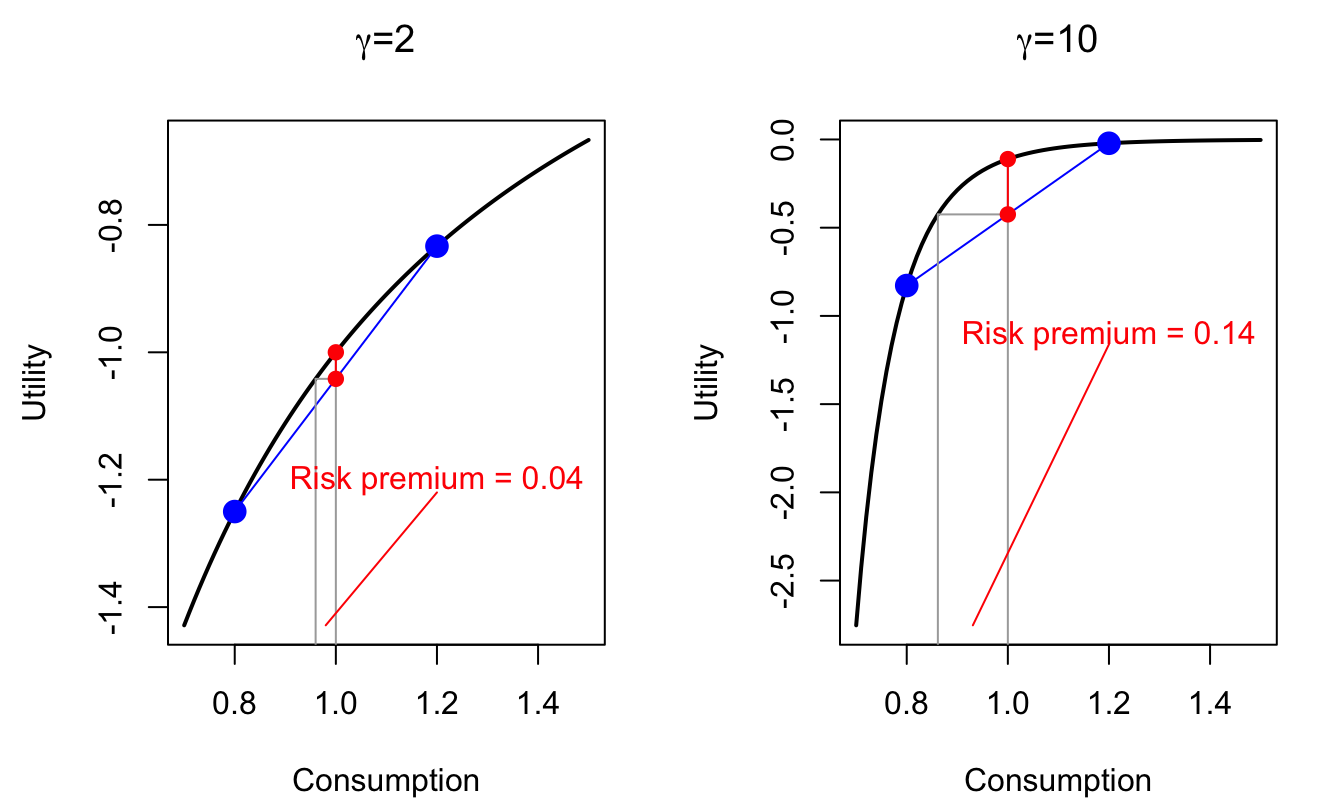
\includegraphics[width=0.95\linewidth]{TSM_files/figure-latex/RRAIESCCAPM-1} \caption{Power utility situation. Illustration of the RRA or the IES.}\label{fig:RRAIESCCAPM}
\end{figure}

\begin{example}[A practical interpretation of the RRA]
\protect\hypertarget{exm:CCAPMRRAinvestment}{}\label{exm:CCAPMRRAinvestment}Consider an agent whose wealth is \(W\). She will consumes only on date \(1\), and features a power utility function \(u\) (see Def. \ref{def:CCAPM}). She can invest, on date \(0\), in an asset whose price is 1 and whose payoff is \(1+\varepsilon\) with probability \(1/2\) and \(1/(1+\varepsilon)\) with probability \(1/2\) (\(\varepsilon\) being small).

Let us compute the optimal share of wealth, denoted by \(\alpha\), that she will invest in the asset. The expected utility is:
\[
\frac{1}{2}u\left[C(1-\alpha)+C\alpha(1+\varepsilon)\right] + \frac{1}{2}u\left[C(1-\alpha)+C\alpha/(1+\varepsilon)\right].
\]
Taking the second-order Taylor expansion of the previous expression and letting \(\varepsilon\) tend to zero, it appears that one has to maximize the following expression:
\[
\alpha u'(C) + \frac{1}{2}C \alpha^2 u''(C).
\]
Hence, the utility is maximized for:
\[
\alpha = - \frac{u'(C)}{C u''(C)} = \frac{1}{RRA}.
\]
\end{example}

The CCAPM is a simple model; it is easy to test once a form for \(u\) has been posited. It is, however, difficult to reconcile with the data (see Subsection \ref{limitationsCCAPM}).

\hypertarget{limitationsCCAPM}{%
\subsection{The limitations of the CCAPM}\label{limitationsCCAPM}}

Three important limitations of the CCAPM approach have been largely documented in the literature:

\begin{enumerate}
\def\labelenumi{\alph{enumi}.}
\tightlist
\item
  Fitting average excess return implies implausible risk aversions (\emph{equity premium puzzle}).
\item
  The resulting risk-free short-term rate is too large unless risk aversion is small (\emph{interest-rate puzzle}).
\item
  It implies maximum Sharpe ratios that are far too low \citep{Hansen_Jagannathan_1991}.
\end{enumerate}

Using \eqref{eq:MRCov} in the power-utility situation, we get the following average excess return:
\begin{eqnarray*}
\mathbb{E}_t(R_{i,t+1} - R_{f,t}) &=& - (1 + R_{f,t}) \mathbb{C}ov_t\left(\delta \dfrac{u'(C_{t+1})}{u'(C_{t})},R_{i,t+1}\right)\\
&\approx& (1 + R_{f,t}) \delta \gamma  \mathbb{C}ov_t\left(\Delta c_{t+1},R_{i,t+1}\right),
\end{eqnarray*}
where \(\Delta c_{t+1} = \log(C_{t+1}/C_t)\).
Because consumption is smooth, the covariance \(\mathbb{C}ov_t\left(\Delta c_{t+1},R_{i,t+1}\right)\) is relatively small (see column ``\(Cov(er_e,\Delta c)\)'\,' of Table \ref{fig:Campbell1}, taken from \citet{Campbell_1999}).
Hence, in order to replicate large average excess return, \(\gamma\) has to be big (see last two columns of Table \ref{fig:Campbell1}).

\begin{figure}

{\centering 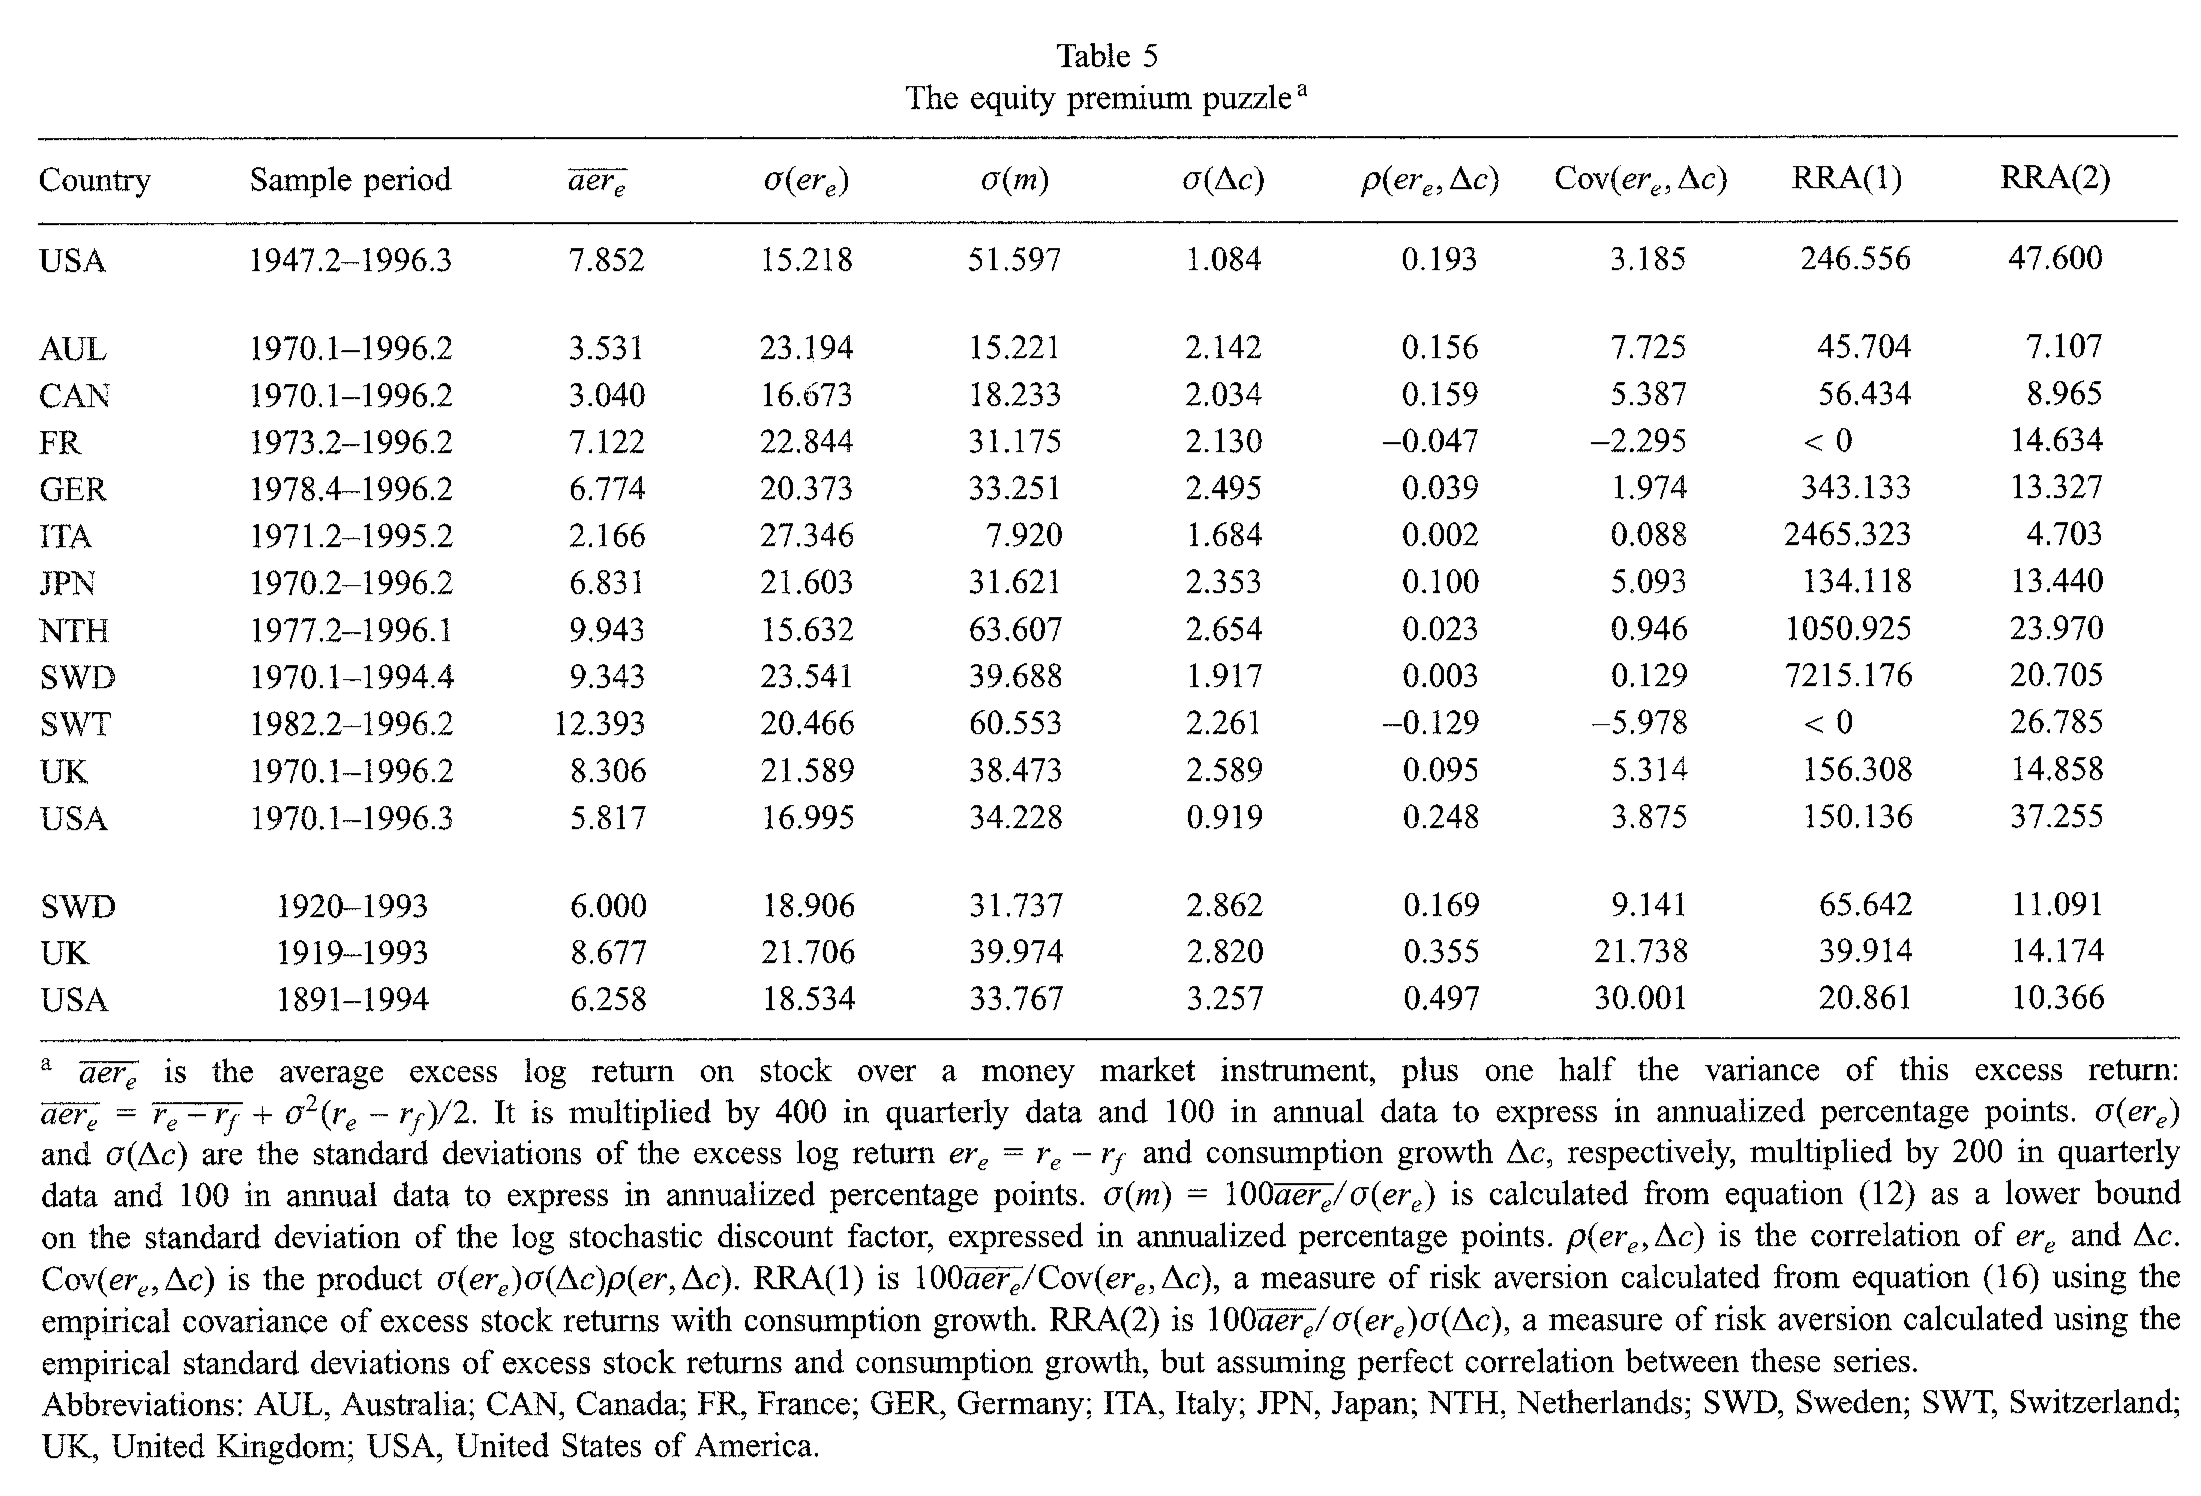
\includegraphics[width=1\linewidth]{figures/table_campbell1999_eqpuzzle} 

}

\caption{Source: Campbell (1999).}\label{fig:Campbell1}
\end{figure}

For sake of comparison: microeconomic study points to estimates of \(\gamma\) in \([1,3]\) (e.g., \citet{Hartley_Lanot_Walker_2014}). This constitutes the \emph{equity premium puzzle} \citep{Mehra_Prescott_1985}.

What if one uses a high risk aversion to get high enough risk premiums? In that case, a novel problem arise \citep{Kandel_Stambaugh_1991}: If people are very risk averse, they want to transfer consumption from high levels to low levels.
In order to allow for a 2\% average increase in \(C_t\), the model predicts that average short-term rate should be high (to prevent people from borrowing too much). Such high interest rates are at odds with the data. This is the \emph{risk-free rate puzzle}.

In the case of the power utility function, the risk aversion is the inverse of the Intertemporal Elasticity of Substitution (Def. \ref{def:IES}):
\[
\mbox{High risk aversion} \Leftrightarrow \mbox{Low IES}.
\]
For given values of the risk-free rates \(R_{f,t}\), a decrease in the IES (increase in \(\gamma\)) leads people to make consumption smoother (see Example \ref{exm:IESsmoothing}).
\[
\frac{1}{1+R_{f,t}} \approx \mathbb{E}_t(\delta (1 - \gamma \Delta c_{t+1})).
\]
Consequently, for the very large \(\gamma\) values needed to adjust average excess returns on equities, agents have a strong desire to smooth consumption (see Example \ref{exm:IESsmoothing}). To reconcile a high risk aversion this with the observed low real interest rate observed on average, it must be that investors are infinitely patients (\emph{risk-free rate puzzle}):
If \(\gamma=10\), \(R_{f,t} \approx 0\%\) and \(\Delta c_{t+1} \approx 2\%\), then \(\delta \approx 1.25\), which is not reasonable.

\begin{example}[IES and smoothing behavior]
\protect\hypertarget{exm:IESsmoothing}{}\label{exm:IESsmoothing}

The agents have a wealth of 1 unit that they consume over two periods. If they consume \(C_1\) in period, they consume \((1+R)(1-C_1)\) in period 2. They feature power-utility time-separable preferences with \(\delta=1\) and \(R=5\%\).

The optimization of the intertemporal utility of the agents imply that \(1/(1+R)=(C_2/C_1)^{-\gamma}\). Hence, the lower the IES, the smoother the consumption path.

\begin{figure}
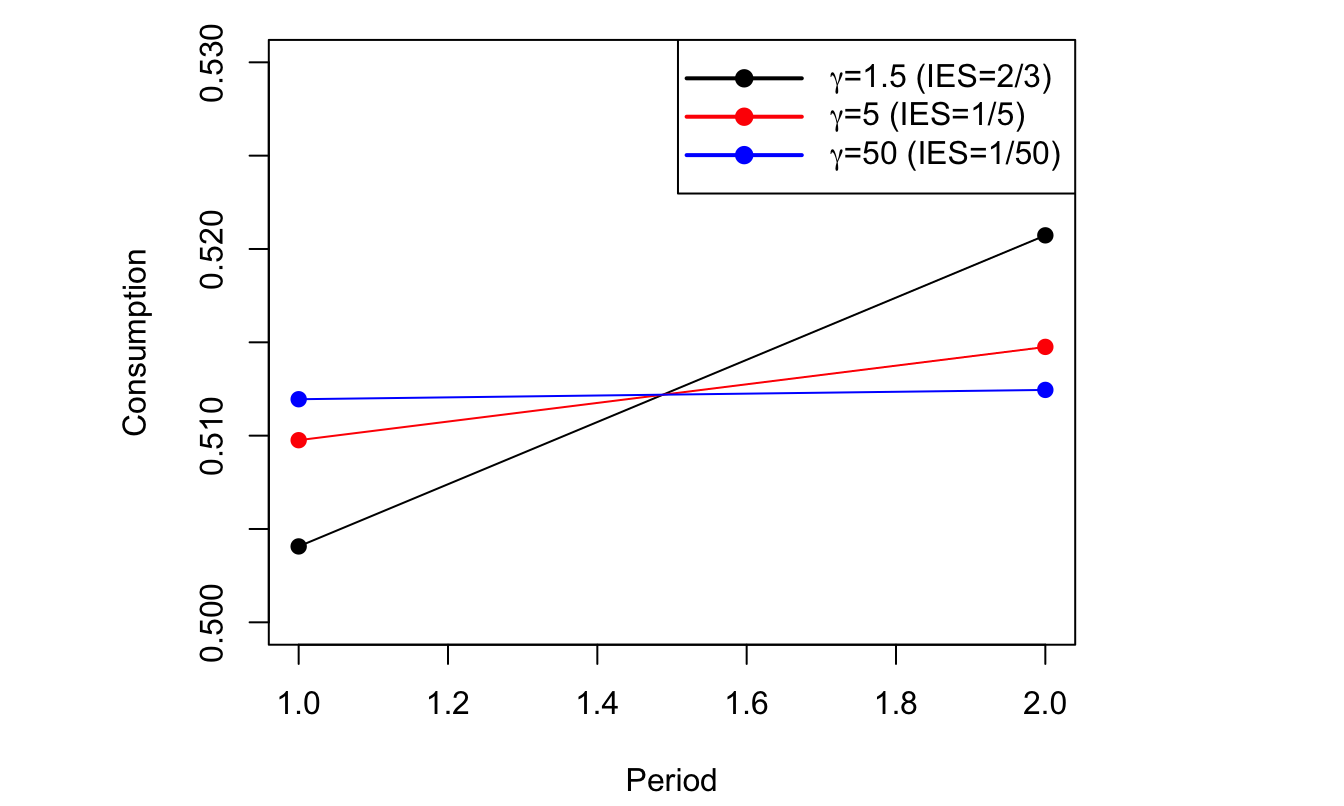
\includegraphics[width=0.95\linewidth]{TSM_files/figure-latex/IESsmooth-1} \caption{Power utility situation. IES and consumption smoothing.}\label{fig:IESsmooth}
\end{figure}

\end{example}

A third problem pertains to the volatility of the SDF. \citet{Grossman_Shiller_1981} and \citet{Hansen_Jagannathan_1991} show that observed Sharpe ratios give lower bounds to the volatility of SDF:
\[
\frac{\sigma_t(\mathcal{M}_{t,t+1})}{\mathbb{E}_t(\mathcal{M}_{t,t+1})} \ge \underbrace{\frac{\mathbb{E}_t(R_{i,t+1}-R_{f,t})}{\sigma_t(R_{i,t+1})}}_{\mbox{Sharpe ratio of asset $i$.}}
\]
The previous inequality results from \eqref{eq:MRCov}, using the fact that \(\mathbb{C}ov(X,Y) \le \sigma(X)\sigma(Y)\).

For postwar U.S. stock market, the Sharpe ratio is about 50\% (see Table \ref{fig:Campbell1}). Given that \(\mathbb{E}_t(\mathcal{M}_{t,t+1}) \approx 1\), this implies that the volatility of the SDF should be at least 50\%.
However, for a power utility function:
\[
\mathcal{M}_{t,t+1}=\delta (C_t/C_{t+1})^\gamma \approx (1 - \gamma \Delta c_{t+1}).
\]
Given the small volatility of \(\Delta c_{t+1}\) (see column \(\sigma(\Delta c)\) in Table \ref{fig:Campbell1}, or use this \href{https://jrenne.shinyapps.io/APModels}{web interface}), \(\gamma\) should be very high for the SDF volatility to be equal to 50\%.

\begin{example}[Econometric Test of the C-CAPM: the GMM approach]
\protect\hypertarget{exm:GMM}{}\label{exm:GMM}

\citet{Hansen_Singleton_1982} have developed and used the General Method of Moments to test the C-CAPM. This approach is based on \eqref{eq:EulerCCAPM}:
\begin{equation}
1 = \color{red}{\mathbb{E}_t}\left( \delta \left(\frac{C_t}{C_{t+1}}\right)^\gamma (1+R_{i,t+1})\right).\label{eq:momentcondi}
\end{equation}
For this to be verified, we must have, for any variable \(z_t\):
\begin{equation}
\color{red}{\mathbb{E}}\left( \underbrace{\left[\delta \left(\frac{C_t}{C_{t+1}}\right)^\gamma (1+R_{i,t+1}) - 1\right] z_t}_{h_{t+1}}\right) = 0,\label{eq:GMM}
\end{equation}
If this is not the case, one can use \(z_t\) to predict \(\delta \left(\frac{C_t}{C_{t+1}}\right)^\gamma (1+R_{i,t+1})\) and \eqref{eq:momentcondi} is not valid. Moment condition: \(\mathbb{E}(h_{t+1})=0\).

Empirical counterpart of the moment condition \eqref{eq:GMM}:
\begin{equation}
\frac{1}{T}\sum_{t=1}^{T} \left[\hat\delta \left(\frac{C_t}{C_{t+1}}\right)^{\hat\gamma} (1+R_{i,t+1}) - 1\right] \times\underbrace{z_{j,t}}_{\mbox{instrument}} = 0.
\end{equation}
In order to identify \(\delta\) and \(\gamma\), one need at least two such equations (with some \(z_{1,t}\) and \(z_{2,t}\)). \citet{Hansen_Singleton_1982} used lagged values of \(R_{i,t+1}\) as instruments. {[}New York Stock Exchange indexes + indexes for different industries{]}

If we have more than two equations, we are in a situation of over-identification. One can use over-identifying restrictions to test for the model.

THey obtained economically meaningful estimates with \(\gamma\) (\(=-\hat\alpha\) in the table below) close to unity (although with a large standard error) and \(\delta\) (\(=\hat\beta\) in the table below) slightly smaller than unity. However, when applied to more than one stock index, the over-identifying restrictions are generally rejected. The data reject the simple version of CCAPM.

\begin{figure}

{\centering 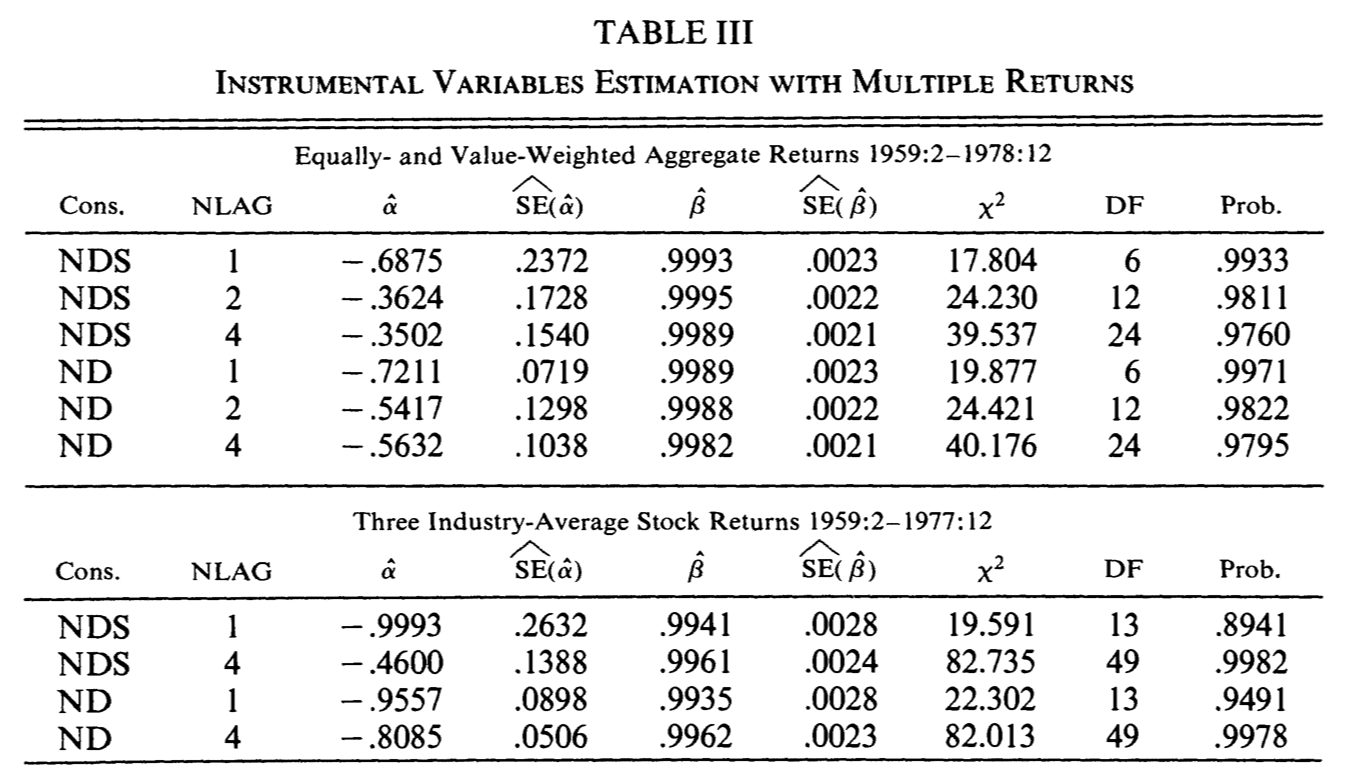
\includegraphics[width=1\linewidth]{figures/tableHansenSingleton82A} 

}

\caption{Source: Hansen and Singleton (1982).}\label{fig:HansenSinfgleton1982}
\end{figure}

\end{example}

\hypertarget{c-capm-that-bad}{%
\subsection{C-CAPM: That bad?}\label{c-capm-that-bad}}

Some studies show that the CCAPM-based puzzles are somehow alleviated when considering longer investment horizons. Indeed, stocks and consumption are more correlated at low frequencies (see, e.g., this \href{https://jrenne.shinyapps.io/APModels}{web interface}). Hence equity-premium puzzle a little less strong for longer horizons (e.g., \citet{DANIEL_MARSHALL_1997}). \citet{Jagannathan_Wang_2007} find that the CCAPM performs reasonably well when using fourth-quarter over fourth-quarter non-durable and service consumption. \citet{Parker_Julliard_2005} study whether the 25 Fama-French portfolios can be priced when considering their exposure to ``long-run'' consumption risk, and find better results than in the standard situation.

According to \citet{Cochrane_2005}, the failure of the C-CAPM models is quantitative, not qualitative. In particular:

\begin{itemize}
\tightlist
\item
  The signs are consistent: since stock market returns are positively correlated with consumption growth, the premiums must be positive (which they are).
\item
  The decrease in bond term premiums over the last decades is consistent with decrease in the correlation between long-term bond excess returns and consumption (see Figure \ref{fig:fredCorrel}, and this \href{https://jrenne.shinyapps.io/APModels}{web interface}).
\item
  In terms of signs, the CAPM is also consistent with currency risk premiums.\footnote{\citet{Lustig_Verdelhan_2007} show that high interest rate currencies depreciate on average when domestic consumption growth is low \(\Rightarrow\) the CAPM predicts higher average return for investments in foreign high-interest rate currencies.}
\end{itemize}

\begin{figure}
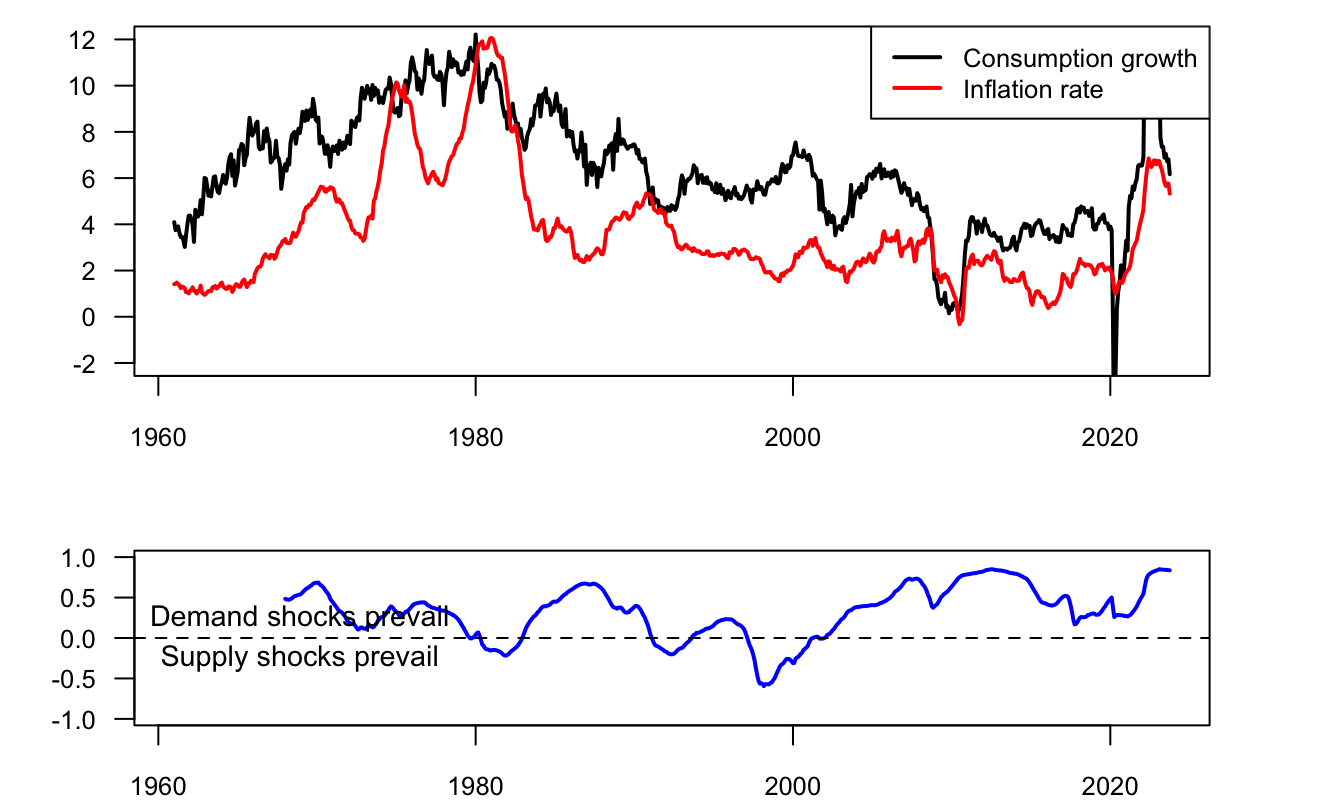
\includegraphics[width=0.95\linewidth]{TSM_files/figure-latex/fredCorrel-1} \caption{Consumption-Inflation correlation. Growth rates are 2-year growth rates. Dynamic correlation is computed using a 7-year rolling window.}\label{fig:fredCorrel}
\end{figure}

\hypertarget{TSCCAPM}{%
\subsection{The term structure of real interest rates in the CCAPM}\label{TSCCAPM}}

This subsection shows how one can develop a term-structure model in the CCAPM context. For that, we need to specify the process followed by consumption. We assume that consumption growth (\(\Delta c_{t}=\log (C_{t}/C_{t-1})\)) follows a Gaussian AR(1) process. Formally:
\[
\Delta c_{t} = \mu + \phi (\Delta c_t - \mu) + \sigma_c \varepsilon_{c,t+1},\quad \varepsilon_{c,t} \sim i.i.d.\mathcal{N}(0,1).
\]

Let's denote by \(r_{t}\) the one-period risk-free real interest rate. We consider the power-utility time-separable preferences context, implying that the real SDF, between dates \(t\) and \(t+1\), is given by \(\delta\exp(-\gamma \Delta c_{t,t+1})\). Applying \eqref{eq:SDF100} to the one-period risk-free real bond, we get:
\begin{eqnarray*}
\mathcal{B}_{t,1} = \exp(-r_{t}) &=& \mathbb{E}_t [ \delta \exp(-\gamma \Delta c_{t+1}) \underbrace{\times 1}_{= x_{i,t+1}} ]\\
&=& \delta \exp\left(-\gamma(\mu + \phi (\Delta c_t - \mu))+\frac{\gamma^2\sigma_c^2}{2}\right).
\end{eqnarray*}
As a result, the short-term real rate is given by
\begin{equation}
r_{t} = \underbrace{- \log(\delta) + \gamma \mu (1-\phi)  - \frac{\gamma^2\sigma_c^2}{2}}_{=\eta_0} + \underbrace{\gamma \phi}_{=\eta_1} \Delta c_t.\label{eq:rCCAPM}
\end{equation}
To price longer-term real bonds, one can use \eqref{eq:SDF100} iteratively. For instance, for \(h=2\):
\begin{eqnarray*}
\mathcal{B}_{t,2} &=&  \mathbb{E}_t \left[ \delta \exp(-\gamma \Delta c_{t+1}) \color{blue}{\mathcal{B}_{t+1,1}} \right]\\
&=& \mathbb{E}_t \big[ \delta \exp(-\gamma \Delta c_{t+1}) \color{blue}{\mathbb{E}_{t+1} \big[ \delta \exp(-\gamma \Delta c_{t+2}) \underbrace{\times 1}_{=\mathcal{B}_{t+2,0}} \big]} \big]\\
&=& \mathbb{E}_t \left[ \delta^2 \exp(-\gamma \Delta c_{t+1} - \gamma \Delta c_{t+2}) \right].
\end{eqnarray*}
Further, for \(h>1\):
\begin{equation}
\mathcal{B}_{t,h} = \mathbb{E}_t \left[ \delta^h \exp(-\gamma \Delta c_{t+1} - \gamma \Delta c_{t+2} \dots - \gamma \Delta c_{t+h}) \right].\label{eq:PthCCAPM}
\end{equation}
It is then tempting to say that this price is also equal to
\begin{equation}
\mathcal{B}^{EH}_{t,h} = \mathbb{E}_t \left[ \exp(- r_{t} - r_{t+1} - \dots - r_{t+h-1}) \right],\label{eq:CCAPMEH}
\end{equation}
but this is not true. This would be the case under the expectation hypothesis (see Eq. \eqref{eq:stdbondRFchapterP}).

Take \(\mathcal{B}_{t,2}\) again; we have:
\begin{eqnarray*}
\mathcal{B}_{t,2} &=&  \mathbb{E}_t \left[ \delta \exp(-\gamma \Delta c_{t+1}) \color{blue}{\mathcal{B}_{t+1,1}} \right]\\
&=& \mathbb{E}_t \left[ \delta \exp(-\gamma \Delta c_{t+1}) \color{blue}{\exp(- r_{t+1})}\right]\\
&=& \underbrace{\mathbb{E}_t \left[ \delta \exp(-\gamma \Delta c_{t+1}) \right]}_{=\exp(-r_{t})}\mathbb{E}_t \left[ \exp(- r_{t+1}) \right] + \mathbb{C}ov_t(\exp(-\gamma \Delta c_{t+1}),\exp(- r_{t+1}))\\
&=& \underbrace{\mathbb{E}_t \left[ \exp(- r_{t}- r_{t+1}) \right]}_{= \mathcal{B}^{EH}_{t,2}} + \mathbb{C}ov_t(\exp(-\gamma \Delta c_{t+1}),\exp(- r_{t+1})).
\end{eqnarray*}
Since \(r_{t+1}\) and \(\Delta c_{t+1}\) are correlated (see Eq. \eqref{eq:rCCAPM}), the covariance term is not equal to zero, which gives rise to term premiums. This is illustrated by Figure \ref{fig:TSMCCAPM}. This figure simulates a path of the real short term rate and shows, for different dates \(t\), the term structures of \(r_{t,h} = -1/h \log \mathcal{B}_{t,h}\) (in red) and of \(r_{t,h}^{EH}= -1/h \log \mathcal{B}^{EH}_{t,h}\) (in blue). (The computation of these yields is based on \eqref{eq:PthCCAPM} and \eqref{eq:CCAPMEH}, using Proposition \ref{prp:reverseMLT},\footnote{In particular, we have (from \eqref{eq:CCAPMEH}):
  \begin{eqnarray}
  r^{EH}_{t,h} &=& -\frac{1}{h} \log \mathbb{E}_t \left[ \exp(- r_{t} - r_{t+1} - \dots - r_{t+h-1}) \right] \\
  &=& \eta_0 -\frac{1}{h} \log \mathbb{E}_t \left[ \exp(  - \eta_1 \Delta c_{t+1} - \dots - \eta_1 \Delta c_{t+h-1}) \right],
  \end{eqnarray}
  where \(\eta_0\) and \(\eta_1\) are defined in \eqref{eq:rCCAPM}.} exploiting that \(\Delta c_t\) follows an affine process.)

Note that the (real) term premiums are negative, which is typical in the context of equilibrium term structure models \citep{Piazzesi_Schneider_2007}. Indeed, in these models, it is often that case that \(\Delta c_{t+1}\) and \(r_{t+1}\) are positively correlated, which implies here that the covariance term is positive, and therefore that \(r_{t,2} < r_{t,2}^{EH}\) (where \(r_{t,2}^{EH} = -1/2 \log \mathcal{B}^{EH}_{t,2}\)).

\begin{Shaded}
\begin{Highlighting}[]
\FunctionTok{library}\NormalTok{(AEC);}\FunctionTok{library}\NormalTok{(TSModels)}
\NormalTok{phi }\OtherTok{\textless{}{-}} \FloatTok{0.6}\NormalTok{;mu }\OtherTok{\textless{}{-}} \FloatTok{0.01}
\NormalTok{sigma.bar }\OtherTok{\textless{}{-}}\NormalTok{ .}\DecValTok{01} \CommentTok{\# unconditional std dev of growth}
\NormalTok{sigma2  }\OtherTok{\textless{}{-}}\NormalTok{ sigma.bar}\SpecialCharTok{\^{}}\DecValTok{2} \SpecialCharTok{*}\NormalTok{ (}\DecValTok{1} \SpecialCharTok{{-}}\NormalTok{ phi}\SpecialCharTok{\^{}}\DecValTok{2}\NormalTok{)}
\NormalTok{sigma.c }\OtherTok{\textless{}{-}} \FunctionTok{sqrt}\NormalTok{(sigma2)}
\NormalTok{gamma   }\OtherTok{\textless{}{-}} \DecValTok{10}
\NormalTok{delta   }\OtherTok{\textless{}{-}} \FloatTok{0.99}
\CommentTok{\# Determine specification of real short{-}term rate:}
\NormalTok{eta}\FloatTok{.0} \OtherTok{\textless{}{-}} \SpecialCharTok{{-}}\FunctionTok{log}\NormalTok{(delta) }\SpecialCharTok{+}\NormalTok{ mu }\SpecialCharTok{*}\NormalTok{ gamma }\SpecialCharTok{*}\NormalTok{ (}\DecValTok{1} \SpecialCharTok{{-}}\NormalTok{ phi) }\SpecialCharTok{{-}} 
\NormalTok{  gamma}\SpecialCharTok{\^{}}\DecValTok{2} \SpecialCharTok{*}\NormalTok{ sigma.c}\SpecialCharTok{\^{}}\DecValTok{2} \SpecialCharTok{/} \DecValTok{2}
\NormalTok{eta}\FloatTok{.1} \OtherTok{\textless{}{-}}\NormalTok{ gamma }\SpecialCharTok{*}\NormalTok{ phi}
\CommentTok{\# Specify the model:}
\NormalTok{psi.parameterization }\OtherTok{\textless{}{-}} \FunctionTok{list}\NormalTok{(}
  \AttributeTok{mu =} \FunctionTok{matrix}\NormalTok{(mu }\SpecialCharTok{*}\NormalTok{ (}\DecValTok{1}\SpecialCharTok{{-}}\NormalTok{phi)),}
  \AttributeTok{Phi =} \FunctionTok{matrix}\NormalTok{(phi),}
  \AttributeTok{Sigma =} \FunctionTok{matrix}\NormalTok{(sigma.c}\SpecialCharTok{\^{}}\DecValTok{2}\NormalTok{))}
\CommentTok{\# Use reverse{-}order multi{-}horizon LT to price ZC bonds:}
\NormalTok{h }\OtherTok{=} \DecValTok{10} \CommentTok{\# maximum maturity}
\NormalTok{u2 }\OtherTok{\textless{}{-}} \FunctionTok{matrix}\NormalTok{(}\SpecialCharTok{{-}}\NormalTok{gamma)}
\NormalTok{u1 }\OtherTok{\textless{}{-}} \FunctionTok{matrix}\NormalTok{(}\SpecialCharTok{{-}}\NormalTok{gamma)}
\NormalTok{AB }\OtherTok{\textless{}{-}} \FunctionTok{reverse.MHLT}\NormalTok{(psi.GaussianVAR,u1,u2,}\AttributeTok{H=}\NormalTok{h,psi.parameterization)}
\NormalTok{a.h }\OtherTok{\textless{}{-}} \SpecialCharTok{{-}}\FunctionTok{c}\NormalTok{(AB}\SpecialCharTok{$}\NormalTok{A)}\SpecialCharTok{/}\NormalTok{(}\DecValTok{1}\SpecialCharTok{:}\NormalTok{h)}
\NormalTok{b.h }\OtherTok{\textless{}{-}} \SpecialCharTok{{-}} \FunctionTok{log}\NormalTok{(delta) }\SpecialCharTok{+} \SpecialCharTok{{-}}\FunctionTok{c}\NormalTok{(AB}\SpecialCharTok{$}\NormalTok{B)}\SpecialCharTok{/}\NormalTok{(}\DecValTok{1}\SpecialCharTok{:}\NormalTok{h)}
\CommentTok{\# Under EH:}
\NormalTok{u2 }\OtherTok{\textless{}{-}} \FunctionTok{matrix}\NormalTok{(}\SpecialCharTok{{-}}\NormalTok{ eta}\FloatTok{.1}\NormalTok{)}
\NormalTok{u1 }\OtherTok{\textless{}{-}} \FunctionTok{matrix}\NormalTok{(}\DecValTok{0}\NormalTok{)}
\NormalTok{AB }\OtherTok{\textless{}{-}} \FunctionTok{reverse.MHLT}\NormalTok{(psi.GaussianVAR,u1,u2,}\AttributeTok{H=}\NormalTok{h,psi.parameterization)}
\NormalTok{a.h.EH }\OtherTok{\textless{}{-}} \SpecialCharTok{{-}}\FunctionTok{c}\NormalTok{(AB}\SpecialCharTok{$}\NormalTok{A }\SpecialCharTok{{-}}\NormalTok{ eta}\FloatTok{.1}\NormalTok{)}\SpecialCharTok{/}\NormalTok{(}\DecValTok{1}\SpecialCharTok{:}\NormalTok{h)}
\NormalTok{b.h.EH }\OtherTok{\textless{}{-}}\NormalTok{ eta}\FloatTok{.0} \SpecialCharTok{{-}} \FunctionTok{c}\NormalTok{(AB}\SpecialCharTok{$}\NormalTok{B)}\SpecialCharTok{/}\NormalTok{(}\DecValTok{1}\SpecialCharTok{:}\NormalTok{h)}
\CommentTok{\# Simulate growth:}
\NormalTok{x.sim }\OtherTok{\textless{}{-}} \FunctionTok{sim.arma}\NormalTok{(mu}\SpecialCharTok{*}\NormalTok{(}\DecValTok{1}\SpecialCharTok{{-}}\NormalTok{phi),phi,}\AttributeTok{theta=}\FunctionTok{c}\NormalTok{(}\DecValTok{1}\NormalTok{),sigma.c,}
                  \AttributeTok{T=}\DecValTok{100}\NormalTok{,mu,}\AttributeTok{nb.sim=}\DecValTok{1}\NormalTok{)}
\NormalTok{r.t   }\OtherTok{\textless{}{-}}\NormalTok{ (eta}\FloatTok{.0} \SpecialCharTok{+}\NormalTok{ eta}\FloatTok{.1} \SpecialCharTok{*}\NormalTok{ x.sim)}
\CommentTok{\# Prepare plots:}
\FunctionTok{par}\NormalTok{(}\AttributeTok{mfrow=}\FunctionTok{c}\NormalTok{(}\DecValTok{1}\NormalTok{,}\DecValTok{1}\NormalTok{));}\FunctionTok{par}\NormalTok{(}\AttributeTok{plt=}\FunctionTok{c}\NormalTok{(.}\DecValTok{1}\NormalTok{,.}\DecValTok{95}\NormalTok{,.}\DecValTok{2}\NormalTok{,.}\DecValTok{95}\NormalTok{))}
\FunctionTok{plot}\NormalTok{(r.t,}\AttributeTok{type=}\StringTok{"l"}\NormalTok{,}\AttributeTok{xlab=}\StringTok{"time"}\NormalTok{,}\AttributeTok{ylab=}\StringTok{""}\NormalTok{,}\AttributeTok{ylim=}\FunctionTok{c}\NormalTok{(}\FunctionTok{min}\NormalTok{(r.t),}
                                             \FunctionTok{max}\NormalTok{(r.t)}\SpecialCharTok{+}\NormalTok{.}\DecValTok{05}\NormalTok{),}\AttributeTok{las=}\DecValTok{1}\NormalTok{)}
\ControlFlowTok{for}\NormalTok{(t }\ControlFlowTok{in} \FunctionTok{seq}\NormalTok{(}\DecValTok{1}\NormalTok{,T,}\AttributeTok{by=}\DecValTok{10}\NormalTok{))\{}
  \FunctionTok{lines}\NormalTok{(t}\SpecialCharTok{+}\NormalTok{(}\DecValTok{1}\SpecialCharTok{:}\NormalTok{h)}\SpecialCharTok{{-}}\DecValTok{1}\NormalTok{,b.h    }\SpecialCharTok{+}\NormalTok{ a.h    }\SpecialCharTok{*}\NormalTok{ x.sim[t],}\AttributeTok{col=}\StringTok{"red"}\NormalTok{,}\AttributeTok{lwd=}\DecValTok{2}\NormalTok{)}
  \FunctionTok{lines}\NormalTok{(t}\SpecialCharTok{+}\NormalTok{(}\DecValTok{1}\SpecialCharTok{:}\NormalTok{h)}\SpecialCharTok{{-}}\DecValTok{1}\NormalTok{,b.h.EH }\SpecialCharTok{+}\NormalTok{ a.h.EH }\SpecialCharTok{*}\NormalTok{ x.sim[t],}\AttributeTok{col=}\StringTok{"blue"}\NormalTok{,}\AttributeTok{lwd=}\DecValTok{2}\NormalTok{)\}}
\FunctionTok{legend}\NormalTok{(}\StringTok{"topright"}\NormalTok{,}
       \FunctionTok{c}\NormalTok{(}\StringTok{"Short{-}term rate"}\NormalTok{,}\StringTok{"Term structure of real yields"}\NormalTok{,}
         \StringTok{"Term structure of real yields (without risk premiums)"}\NormalTok{),}
       \AttributeTok{lwd=}\FunctionTok{c}\NormalTok{(}\DecValTok{2}\NormalTok{),}\AttributeTok{lty=}\FunctionTok{c}\NormalTok{(}\DecValTok{1}\NormalTok{,}\DecValTok{1}\NormalTok{,}\DecValTok{1}\NormalTok{),}\AttributeTok{col=}\FunctionTok{c}\NormalTok{(}\StringTok{"black"}\NormalTok{,}\StringTok{"red"}\NormalTok{,}\StringTok{"blue"}\NormalTok{),}\AttributeTok{seg.len =} \DecValTok{4}\NormalTok{)}
\end{Highlighting}
\end{Shaded}

\begin{figure}
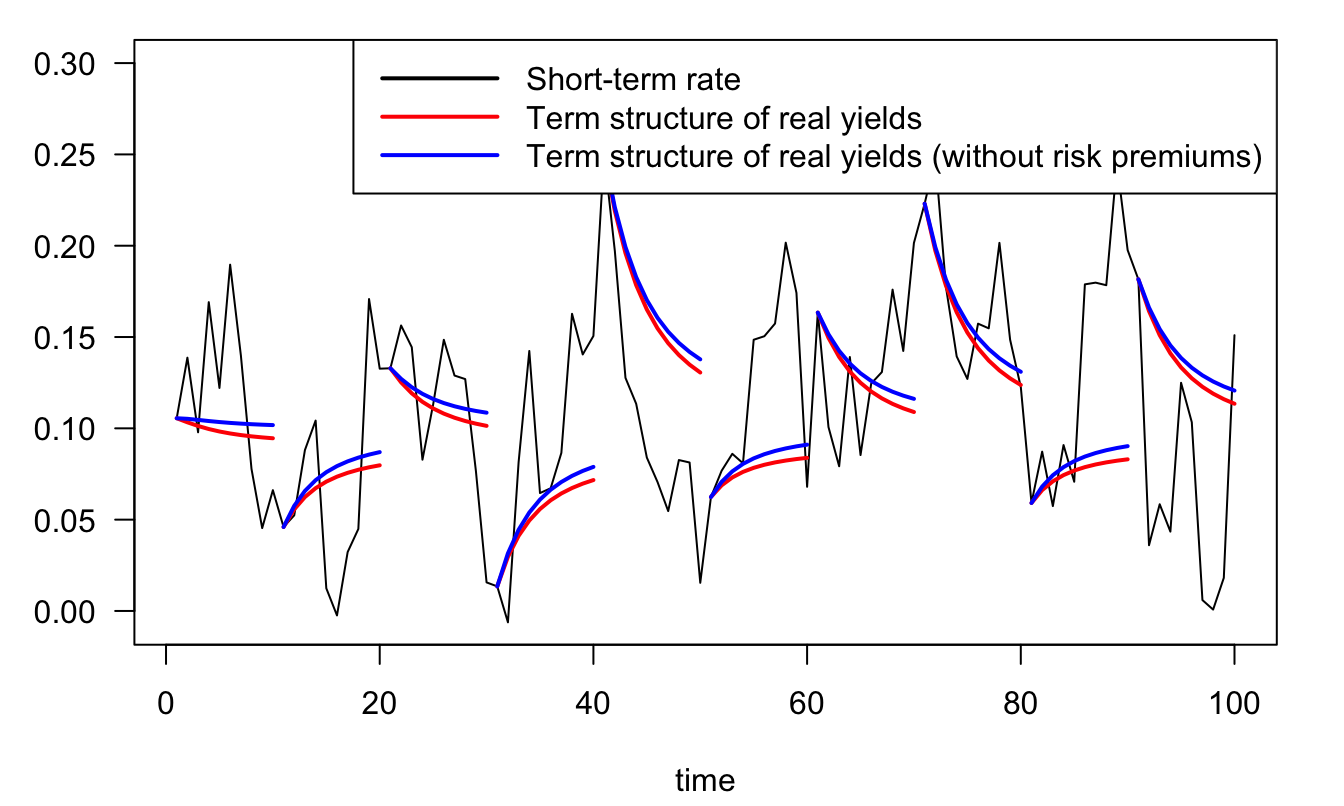
\includegraphics[width=0.95\linewidth]{TSM_files/figure-latex/TSMCCAPM-1} \caption{Term structures of real rates in a small dynamic CCAPM. The parameters are as follows: $\phi=0.6$, $\mu = 0.01$, $\gamma=10$, $\delta = 0.99$, $\sigma_c=0.008$.}\label{fig:TSMCCAPM}
\end{figure}

Let us augment this framework with inflation. Specifically, assume that:
\[
\pi_t = \mu_\pi + \phi_\pi (\pi_{t-1} - \mu_\pi) + \sigma_\pi \varepsilon_{\pi,t} + \sigma_{\pi,c}\varepsilon_{c,t},
\]
where \(\varepsilon_{\pi,t} \sim i.i.d.\,\mathcal{N}(0,1)\) is independent from \(\varepsilon_{c,t+1}\). In that framework, \(\pi_t\) and \(\Delta c_t\) are correlated; specifically:
\[
\mathbb{C}ov_t(\Delta c_{t+1},\pi_{t+1}) = \sigma_{\pi,c}\sigma_{c},
\]
whose sign is that of \(\sigma_{\pi,c}\).

The price of the nominal bond of maturity \(1\) is given by:
\begin{eqnarray*}
&&\mathbb{E}_t(\exp(\log(\delta) -\gamma \Delta c_{t+1}-\pi_{t+1}))\\
&=& \mathbb{E}_t(\exp(\log(\delta)-\gamma [\mu + \phi (\Delta c_t - \mu) + \sigma_c \varepsilon_{c,t+1}] \\
&& - \mu_\pi - \phi_\pi (\pi_{t} - \mu_\pi) - \sigma_\pi \varepsilon_{\pi,t+1} - \sigma_{\pi,c}\varepsilon_{c,t+1}))\\
&=& \exp(\log(\delta)-\gamma \mu (1-\phi) - \mu_\pi(1-\phi_\pi)-\gamma \phi \Delta c_t - \phi_\pi \pi_{t}) \times \\
&& \mathbb{E}_t(\exp( - (\gamma \sigma_c+\sigma_{\pi,c}) \varepsilon_{c,t+1}  - \sigma_\pi \varepsilon_{\pi,t+1})),
\end{eqnarray*}
which leads to the following one-period nominal interest rate:
\begin{eqnarray}
i_t &=& - \log(\delta) +\gamma \mu (1-\phi) + \mu_\pi(1-\phi_\pi) - \frac{1}{2}(\gamma \sigma_c+\sigma_{\pi,c})^2 - \frac{1}{2}\sigma_\pi^2 \nonumber\\ 
&& + \gamma \phi \Delta c_t + \phi_\pi \pi_{t}. \label{eq:nominalCCAPM}
\end{eqnarray}

The price of a nominal bond of maturity \(h\) is:
\begin{eqnarray*}
B_{t,h} &=& \mathbb{E}_t(\delta^{h}\exp(-\gamma (\Delta c_{t+1}+\dots+\Delta c_{t+h}) - \pi_{t+1}-\dots-\pi_{t+h})).
\end{eqnarray*}
This price is a multi-horizon Laplace transform of vector \(w_t = [\Delta c_t,\pi_t]'\), which follows a Gaussian VAR process:
\[
\left[\begin{array}{c}\Delta c_t\\
\pi_t\end{array}\right] = 
\left[\begin{array}{c} \mu (1-\phi)\\
\mu_\pi(1-\phi_\pi)\end{array}\right]+
\left[\begin{array}{cc} \phi & 0\\
0 & \phi_\pi\end{array}\right]\left[\begin{array}{c}\Delta c_{t-1}\\
\pi_{t-1}\end{array}\right]+
\left[\begin{array}{cc} \sigma_c & 0\\
\sigma_{\pi c} & \sigma_\pi\end{array}\right]\left[\begin{array}{c}\varepsilon_{c,t}\\
\varepsilon_{\pi,t}\end{array}\right].
\]

In the following lines of code, we use Proposition \ref{prp:reverseMLT} (i.e.~function \texttt{reverse.MHLT}) to compute the nominal yield curve. We also determine it under the Expectation Hypothesis, using \(i^{EH}_{t,h} = - \log \mathbb{E}_t [\exp(-i_t - \dots - i_{t+h-1})]\).

Figure \ref{fig:TSMCCAPM2} shows the resulting average nominal yield curves, together with the average real yield curves.

\begin{Shaded}
\begin{Highlighting}[]
\NormalTok{mu\_pi }\OtherTok{\textless{}{-}}\NormalTok{ .}\DecValTok{02}\NormalTok{;phi\_pi }\OtherTok{\textless{}{-}}\NormalTok{ .}\DecValTok{8}\NormalTok{;sigma.pi.c }\OtherTok{\textless{}{-}} \SpecialCharTok{{-}}\NormalTok{.}\DecValTok{06}\NormalTok{;sigma.pi   }\OtherTok{\textless{}{-}}\NormalTok{ .}\DecValTok{01}
\CommentTok{\# Determine specification of nominal short{-}term rate:}
\NormalTok{eta.}\FloatTok{0.}\NormalTok{i }\OtherTok{\textless{}{-}} \SpecialCharTok{{-}}\FunctionTok{log}\NormalTok{(delta) }\SpecialCharTok{+}\NormalTok{ mu }\SpecialCharTok{*}\NormalTok{ gamma }\SpecialCharTok{*}\NormalTok{ (}\DecValTok{1} \SpecialCharTok{{-}}\NormalTok{ phi) }\SpecialCharTok{+}\NormalTok{ mu\_pi }\SpecialCharTok{*} 
\NormalTok{  (}\DecValTok{1} \SpecialCharTok{{-}}\NormalTok{ phi\_pi) }\SpecialCharTok{{-}}\NormalTok{ (gamma}\SpecialCharTok{*}\NormalTok{sigma.c }\SpecialCharTok{+}\NormalTok{ sigma.pi.c)}\SpecialCharTok{\^{}}\DecValTok{2}\SpecialCharTok{/}\DecValTok{2} \SpecialCharTok{{-}}\NormalTok{ sigma.pi}\SpecialCharTok{\^{}}\DecValTok{2}\SpecialCharTok{/}\DecValTok{2}
\NormalTok{eta.}\FloatTok{1.}\NormalTok{i }\OtherTok{\textless{}{-}} \FunctionTok{matrix}\NormalTok{(}\FunctionTok{c}\NormalTok{(gamma }\SpecialCharTok{*}\NormalTok{ phi,phi\_pi),}\DecValTok{2}\NormalTok{,}\DecValTok{1}\NormalTok{)}
\CommentTok{\# Specify the model:}
\NormalTok{psi.parameterization }\OtherTok{\textless{}{-}} \FunctionTok{list}\NormalTok{(}
  \AttributeTok{mu =} \FunctionTok{matrix}\NormalTok{(}\FunctionTok{c}\NormalTok{(mu}\SpecialCharTok{*}\NormalTok{(}\DecValTok{1}\SpecialCharTok{{-}}\NormalTok{phi),mu\_pi}\SpecialCharTok{*}\NormalTok{(}\DecValTok{1}\SpecialCharTok{{-}}\NormalTok{phi\_pi)),}\DecValTok{2}\NormalTok{,}\DecValTok{1}\NormalTok{),}
  \AttributeTok{Phi =} \FunctionTok{diag}\NormalTok{(}\FunctionTok{c}\NormalTok{(phi,phi\_pi)),}
  \AttributeTok{Sigma =} \FunctionTok{matrix}\NormalTok{(}\FunctionTok{c}\NormalTok{(sigma.c}\SpecialCharTok{\^{}}\DecValTok{2}\NormalTok{,sigma.c}\SpecialCharTok{*}\NormalTok{sigma.pi.c,sigma.c}\SpecialCharTok{*}
\NormalTok{                     sigma.pi.c,sigma.pi}\SpecialCharTok{\^{}}\DecValTok{2}\SpecialCharTok{+}\NormalTok{sigma.pi.c}\SpecialCharTok{\^{}}\DecValTok{2}\NormalTok{),}\DecValTok{2}\NormalTok{,}\DecValTok{2}\NormalTok{))}
\CommentTok{\# Use reverse{-}order multi{-}horizon LT to price ZC bonds:}
\NormalTok{u2 }\OtherTok{\textless{}{-}} \FunctionTok{matrix}\NormalTok{(}\FunctionTok{c}\NormalTok{(}\SpecialCharTok{{-}}\NormalTok{gamma,}\SpecialCharTok{{-}}\DecValTok{1}\NormalTok{),}\DecValTok{2}\NormalTok{,}\DecValTok{1}\NormalTok{);u1 }\OtherTok{\textless{}{-}} \FunctionTok{matrix}\NormalTok{(}\FunctionTok{c}\NormalTok{(}\SpecialCharTok{{-}}\NormalTok{gamma,}\SpecialCharTok{{-}}\DecValTok{1}\NormalTok{),}\DecValTok{2}\NormalTok{,}\DecValTok{1}\NormalTok{)}
\NormalTok{AB }\OtherTok{\textless{}{-}} \FunctionTok{reverse.MHLT}\NormalTok{(psi.GaussianVAR,u1,u2,}\AttributeTok{H=}\NormalTok{h,psi.parameterization)}
\NormalTok{a.h.i }\OtherTok{\textless{}{-}} \SpecialCharTok{{-}}\FunctionTok{matrix}\NormalTok{(AB}\SpecialCharTok{$}\NormalTok{A,}\DecValTok{2}\NormalTok{,h)}\SpecialCharTok{/}\FunctionTok{t}\NormalTok{(}\FunctionTok{matrix}\NormalTok{((}\DecValTok{1}\SpecialCharTok{:}\NormalTok{h),h,}\DecValTok{2}\NormalTok{))}
\NormalTok{b.h.i }\OtherTok{\textless{}{-}} \SpecialCharTok{{-}}\FunctionTok{log}\NormalTok{(delta) }\SpecialCharTok{+} \SpecialCharTok{{-}}\FunctionTok{c}\NormalTok{(AB}\SpecialCharTok{$}\NormalTok{B)}\SpecialCharTok{/}\NormalTok{(}\DecValTok{1}\SpecialCharTok{:}\NormalTok{h)}
\CommentTok{\# Under EH:}
\NormalTok{u2 }\OtherTok{\textless{}{-}} \FunctionTok{matrix}\NormalTok{(}\SpecialCharTok{{-}}\NormalTok{ eta.}\FloatTok{1.}\NormalTok{i);u1 }\OtherTok{\textless{}{-}} \FunctionTok{matrix}\NormalTok{(}\DecValTok{0}\NormalTok{,}\DecValTok{2}\NormalTok{,}\DecValTok{1}\NormalTok{)}
\NormalTok{AB }\OtherTok{\textless{}{-}} \FunctionTok{reverse.MHLT}\NormalTok{(psi.GaussianVAR,u1,u2,}\AttributeTok{H=}\NormalTok{h,psi.parameterization)}
\NormalTok{a.h.i.EH }\OtherTok{\textless{}{-}} \SpecialCharTok{{-}}\NormalTok{(}\FunctionTok{matrix}\NormalTok{(AB}\SpecialCharTok{$}\NormalTok{A,}\DecValTok{2}\NormalTok{,h)}\SpecialCharTok{{-}}
                \FunctionTok{matrix}\NormalTok{(eta.}\FloatTok{1.}\NormalTok{i,}\DecValTok{2}\NormalTok{,h))}\SpecialCharTok{/}\FunctionTok{t}\NormalTok{(}\FunctionTok{matrix}\NormalTok{((}\DecValTok{1}\SpecialCharTok{:}\NormalTok{h),h,}\DecValTok{2}\NormalTok{))}
\NormalTok{b.h.i.EH }\OtherTok{\textless{}{-}}\NormalTok{ eta.}\FloatTok{0.}\NormalTok{i }\SpecialCharTok{{-}} \FunctionTok{c}\NormalTok{(AB}\SpecialCharTok{$}\NormalTok{B)}\SpecialCharTok{/}\NormalTok{(}\DecValTok{1}\SpecialCharTok{:}\NormalTok{h)}
\CommentTok{\# Average yield curves:}
\NormalTok{avg.i.h    }\OtherTok{\textless{}{-}}\NormalTok{ b.h.i    }\SpecialCharTok{+} \FunctionTok{matrix}\NormalTok{(}\FunctionTok{c}\NormalTok{(mu,mu\_pi),}\DecValTok{1}\NormalTok{,}\DecValTok{2}\NormalTok{) }\SpecialCharTok{\%*\%}\NormalTok{ a.h.i}
\NormalTok{avg.i.h.EH }\OtherTok{\textless{}{-}}\NormalTok{ b.h.i.EH }\SpecialCharTok{+} \FunctionTok{matrix}\NormalTok{(}\FunctionTok{c}\NormalTok{(mu,mu\_pi),}\DecValTok{1}\NormalTok{,}\DecValTok{2}\NormalTok{) }\SpecialCharTok{\%*\%}\NormalTok{ a.h.i.EH}
\FunctionTok{plot}\NormalTok{(}\FunctionTok{c}\NormalTok{(avg.i.h),}\AttributeTok{type=}\StringTok{"l"}\NormalTok{,}\AttributeTok{lwd=}\DecValTok{2}\NormalTok{,}\AttributeTok{col=}\StringTok{"red"}\NormalTok{,}\AttributeTok{lty=}\DecValTok{3}\NormalTok{,}
     \AttributeTok{ylim=}\FunctionTok{c}\NormalTok{(}\FloatTok{0.08}\NormalTok{,}\FunctionTok{max}\NormalTok{(avg.i.h)),}
     \AttributeTok{xlab=}\StringTok{"maturity"}\NormalTok{,}\AttributeTok{ylab=}\StringTok{"yield"}\NormalTok{,}\AttributeTok{las=}\DecValTok{1}\NormalTok{);}\FunctionTok{grid}\NormalTok{()}
\FunctionTok{lines}\NormalTok{(}\FunctionTok{c}\NormalTok{(avg.i.h.EH),}\AttributeTok{type=}\StringTok{"l"}\NormalTok{,}\AttributeTok{lwd=}\DecValTok{2}\NormalTok{,}\AttributeTok{col=}\StringTok{"blue"}\NormalTok{,}\AttributeTok{lty=}\DecValTok{3}\NormalTok{)}
\FunctionTok{lines}\NormalTok{(b.h}\SpecialCharTok{+}\NormalTok{a.h}\SpecialCharTok{*}\NormalTok{mu,}\AttributeTok{lwd=}\DecValTok{2}\NormalTok{,}\AttributeTok{col=}\StringTok{"red"}\NormalTok{)}
\FunctionTok{lines}\NormalTok{(b.h.EH}\SpecialCharTok{+}\NormalTok{a.h.EH}\SpecialCharTok{*}\NormalTok{mu,}\AttributeTok{lwd=}\DecValTok{2}\NormalTok{,}\AttributeTok{col=}\StringTok{"blue"}\NormalTok{)}
\FunctionTok{legend}\NormalTok{(}\StringTok{"bottomleft"}\NormalTok{,}
       \FunctionTok{c}\NormalTok{(}\StringTok{"with risk premiums"}\NormalTok{,}
         \StringTok{"without risk premiums"}\NormalTok{),}
       \AttributeTok{lwd=}\FunctionTok{c}\NormalTok{(}\DecValTok{2}\NormalTok{),}\AttributeTok{lty=}\FunctionTok{c}\NormalTok{(}\DecValTok{1}\NormalTok{,}\DecValTok{1}\NormalTok{),}\AttributeTok{col=}\FunctionTok{c}\NormalTok{(}\StringTok{"red"}\NormalTok{,}\StringTok{"blue"}\NormalTok{),}\AttributeTok{seg.len =} \DecValTok{3}\NormalTok{)}
\end{Highlighting}
\end{Shaded}

\begin{figure}
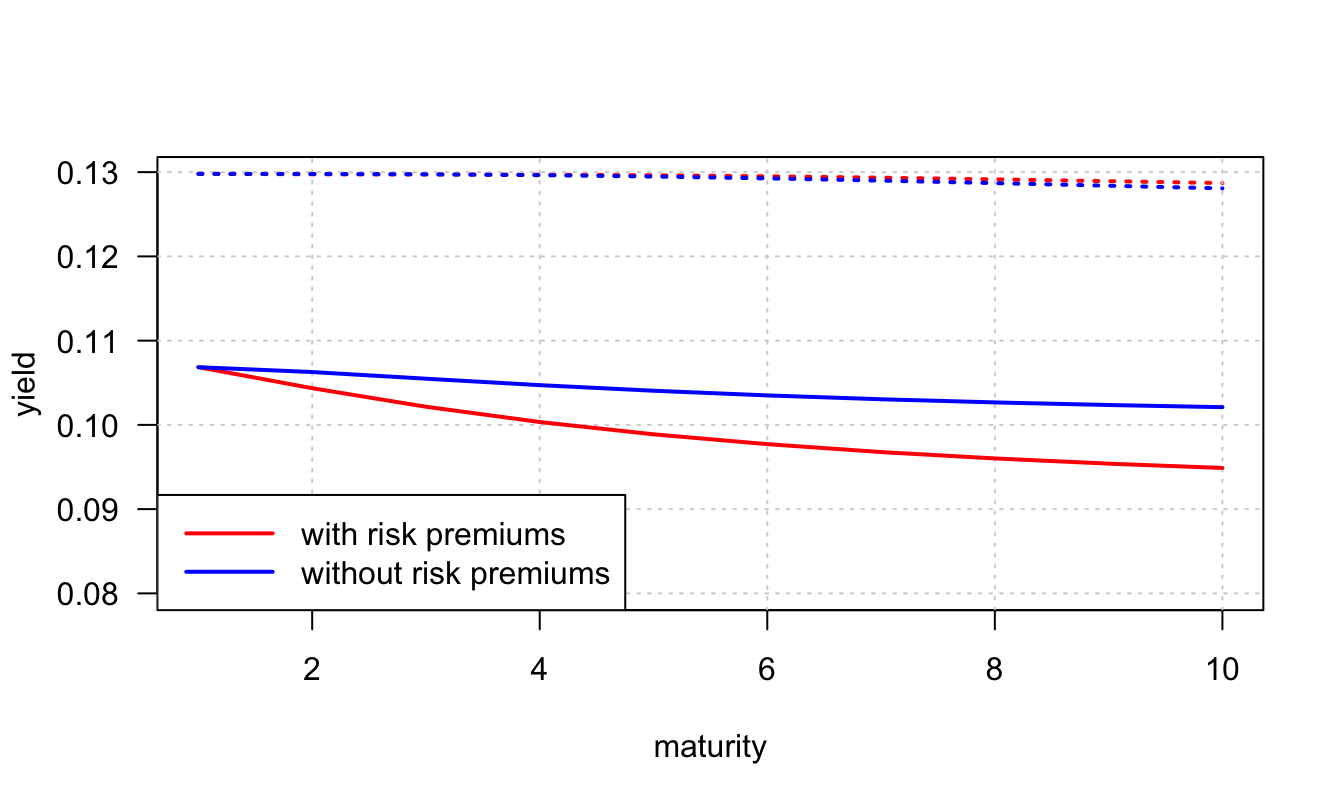
\includegraphics[width=0.95\linewidth]{TSM_files/figure-latex/TSMCCAPM2-1} \caption{Average yield curves (solid lines: real rates; dotted lines: nominal rates), using $\mu_\pi = 0.02$, $\phi_\pi=0.8$, $\sigma_{\pi,c}=-0.6$, and $\sigma_\pi=0.01$.}\label{fig:TSMCCAPM2}
\end{figure}

Using the notations used in Subsection \ref{RiskFreeGaussian}, the (nominal) SDF is of the form:
\[
\mathcal{M}_{t,t+1} = \exp(-i_t + \alpha_0'w_{t+1} - \psi_{t}(\alpha_0)),
\]
where \(\psi_t\) denotes the conditional log-Laplace transform of \(w_t\) and where \(\alpha_0 = [-\gamma,-1]'\). Using the results of Subsection \ref{RiskFreeGaussian}, the risk-neutral dynamics of \(w_t\) is of the form:
\[
\left[\begin{array}{c}\Delta c_t\\
\pi_t\end{array}\right] = 
\underbrace{\left[\begin{array}{c} \mu (1-\phi)\\
\mu_\pi(1-\phi_\pi)\end{array}\right]+\Sigma \lambda_0}_{=\mu^{\mathbb{Q}}}+
\left[\begin{array}{cc} \phi & 0\\
0 & \phi_\pi\end{array}\right]\left[\begin{array}{c}\Delta c_{t-1}\\
\pi_{t-1}\end{array}\right]+
\left[\begin{array}{cc} \sigma_c & 0\\
\sigma_{\pi c} & \sigma_\pi\end{array}\right]\left[\begin{array}{c}\varepsilon_{c,t}^*\\
\varepsilon_{\pi,t}^*\end{array}\right],
\]
where \(\Sigma = \left[\begin{array}{cc}\sigma_c^2&\sigma_c\sigma_{\pi,c}\\ \sigma_c\sigma_{\pi,c}&\sigma_{\pi}^2 \end{array}\right]\) and \([\varepsilon_{c,t}^*,\varepsilon_{\pi,t}^*]'\sim \mathcal{N}'^{\mathbb{Q}}(0,Id)\).

\begin{quote}
Use the risk-neutral dynamics of \(w_t\) to compute the nominal yield curve, using that \(i_{t,h} = - \log \mathbb{E}^{\mathbb{Q}}_t [\exp(-i_t - \dots - i_{t+h-1})]\). (This should give the same results as before.)
\end{quote}

\hypertarget{recursive-utilities}{%
\section{Recursive Utilities}\label{recursive-utilities}}

Given the limitations of consumption-based models, one has questioned the utility function. But the functional form is not really an issue: in the time-separable framework, linearized and non-linearized models behave relatively similarly. (Utility functions are monotonously increasing with negative second order derivatives, so they all have the same broad shapes.) What about the arguments of the utility function? The idea is the following: the marginal utility of consumption may not depend \emph{only} on today's consumption. Pricing implications are very different when the marginal utility of consumption depends on past or (expected) future consumption. In particular, this will permit to address the following limitations of expected-utility time-separable preferences (Def. \ref{def:EUTSpref}):

\begin{itemize}
\tightlist
\item
  No premium for early resolution of uncertainty (i.e., as of date \(t\), the promise to know \(C_{t+h}\) at date \(t+1\) has no value).
\item
  No utility effect of potential autocorrelation in \(C_t\) (i.e., each stream of consumption intervenes independently from the others in the utility computation).
\end{itemize}

\emph{Non-separability over time} means that the marginal utility of today's consumption depends on past consumption. In other words, what you consumed yesterday can have an impact on how you feel about more consumption today.\footnote{As \citet{Cochrane_2005} puts it: ``\emph{Yesterday's pizza lowers the marginal utility for another pizza today.}'')}

\hypertarget{habit-formation}{%
\subsection{Habit formation}\label{habit-formation}}

A first example of recursive utilities is that of \emph{habit formation} \citep{Campbell_Shiller_1999}, where
\begin{equation}
U_t = \sum_{s=t}^{\infty} \delta^{s-t} u(C_s - X_s) \quad where \quad X_t = \rho X_{t-1} + \lambda C_t.\label{eq:Uhabitnonstoch}
\end{equation}

The date-\(t\) utility associated with a level of consumption \(C_t\), that is \(u(C_t - X_t)\), is lower is you already had a high level of consumption at date \(t-1\) (high \(X_t\)).
\[
U_t = \sum_{h=0}^{\infty} \delta^{h}u\left(C_{t+h} - \lambda \sum_{j=0}^\infty \rho^j C_{t+h-j}\right).
\]

A fall in consumption hurts after a few years of good times (even if the same level of consumption would have been very pleasant if it arrived after a few bad years).

If one assumes that \(X_t\) is exogenous---a case referred to as \emph{external habits}---and if \(u(Z)=Z^{1-\gamma}/(1-\gamma)\) (Def. \ref{def:CCAPM}) then:\footnote{Without the external habit assumption, the Euler equation (equilibrium relationship between risk-free short-term rate and marginal utilities) is far less tractable:
  \begin{eqnarray*}
  && 0 = \Delta U_t / \varepsilon =\\
  && \underbrace{ - u'\left(C_{t} - \lambda \sum_{j=0}^\infty \rho^j C_{t-j}\right) + \lambda  \sum_{h=0}^{\infty} \rho^h \delta^{h}u'\left(C_{t+h} - \lambda \sum_{j=0}^\infty \rho^j C_{t+h-j}\right)}_{\mbox{decrease in utility stemming from lower consumption at date $t$}} +\\
  && \underbrace{\delta(1+R_{f,t}) u'\left(C_{t+1} - \lambda \sum_{j=0}^\infty \rho^j C_{t+1-j}\right) - \lambda (1+R_{f,t}) \sum_{h=1}^{\infty} \rho^h \delta^{h}u'\left(C_{t+h} - \lambda \sum_{j=0}^\infty \rho^j C_{t+h-j}\right)}_{\mbox{increase in utility stemming from higher consumption at date $t+1$}},
  \end{eqnarray*}
  which is obtained by considering a marginal decrease in \(C_t\) by \(\varepsilon\) and an increase in \(C_{t+1}\) by \(\varepsilon(1+R_{f,t})\).}
\begin{equation}
\mathcal{M}_{t,t+1} = \delta \left( \frac{C_{t+1}}{C_t} \right)^{-\gamma}\left( \frac{S_{t+1}}{S_t} \right)^{-\gamma},\label{eq:Mhabit}
\end{equation}
where \(S_t = (C_t - X_t)/C_t\). This extends the standard power utility case by adding an additional state variable (\(X_t\)). In this model, recessions are periods where consumption is closer to habits (otherwise it is higher). SDF specifications of the type of \eqref{eq:Mhabit} can arise in more general contexts (not necessarily habits); \(S_t\) may for instance reflect a business-cycle-related variable.

\begin{example}[Comparisons of situations according to habit preferences]
\protect\hypertarget{exm:habit}{}\label{exm:habit}To illustrate, consider the following context (with no uncertainty):
\[
\delta = 1,\quad \gamma = 3, \quad \rho = 0.5, \quad \lambda = 0.49.
\]
Let's define two sequences of interest rates (A and B):
\begin{eqnarray*}
R^{(A)}_1 &=&R^{(A)}_2 =\dots=R^{(A)}_5 =  7\% \\
R^{(A)}_6 &=&R^{(A)}_7 =R^{(A)}_8 =  -20\%
\end{eqnarray*}
and
\[
R^{(B)}_1 =R^{(B)}_2 =\dots=R^{(B)}_{10} =  2.5\%.
\]
For each sequence, we compute the resulting sequence of consumption, with \(C_1=1\).
Results on next slide.

\begin{figure}
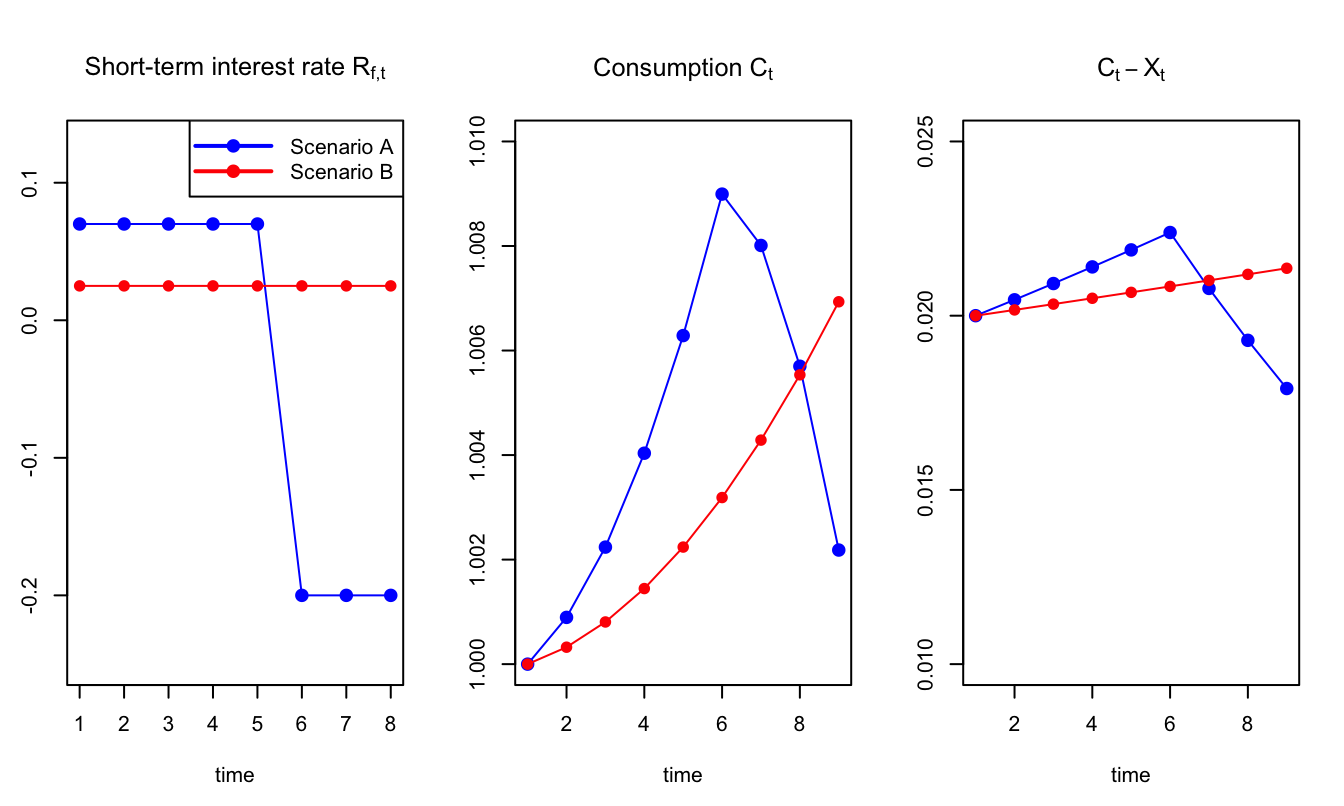
\includegraphics[width=0.95\linewidth]{TSM_files/figure-latex/Habits1-1} \caption{Comparison of Scenarios A and B using habit-based preferences.}\label{fig:Habits1}
\end{figure}

The utility associated to Scenario A (\(-10779\)) is lower than that associated to Scenario B (\(-10542\)).
Without the \(X_t\) term, the utility of Scenario A would be higher than that of Scenario B.
\end{example}

\hypertarget{limitations-of-the-habit-model-for-long-horizons}{%
\subsection{Limitations of the habit model for long-horizons}\label{limitations-of-the-habit-model-for-long-horizons}}

The models based on \eqref{eq:Mhabit} generally works well in the short-run but not in the long-run. Let us consider the horizon-\(h\) SDF:
\[
\mathcal{M}_{t,t+h} = \delta \left( \frac{C_{t+h}}{C_t} \right)^{-\gamma}\left( \frac{S_{t+h}}{S_t} \right)^{-\gamma},
\]
In order to generate a high maximum Sharpe ratio for long horizons, we need a high conditional volatility of \(\mathcal{M}_{t,t+h}\).
If \(c_t\) follows a random walk, the volatility of \(\left( \frac{C_{t+h}}{C_t} \right)^{-\gamma}\) is approximately linear in \(h\).
By contrast, if \(S_t^{-\gamma}\) is stationary, then the conditional volatility of \(\left( \frac{S_{t+h}}{S_t} \right)^{-\gamma}\) does not increase indefinitely with \(h\) (though this term may substantially contribute to the short-run SDF volatility). As a result, these models do not solve the problems pertaining to the standard power-utility time-separable model for long-run horizons.

\hypertarget{EZsection}{%
\subsection{Epstein-Zin preferences}\label{EZsection}}

\citet{Epstein_Zin_1989} have proposed a framework where there is a premium for early resolution and where the time composition of risk matters.

\begin{definition}[Epstein and Zin (1989) Preferences]
\protect\hypertarget{def:EZ}{}\label{def:EZ}Epstein-Zin preferences are defined recursively over current (known) consumption and a certainty equivalent
\(R_t(U_{t+1})\) of future utility:
\[
U_{t} = F(C_t,R_t(U_{t+1})),
\]
where \(R_t(U_{t+1})\), the certainty equivalent of \(U_{t+1}\), is:
\[
R_t(U_{t+1}) = G^{-1}[\mathbb{E}_t(G(U_{t+1}))],
\]
where \(F\) and \(G\) are increasing and concave functions, and where \(F\) is homogenous of degree one.
\end{definition}

\begin{quote}
We have \(R_t(U_{t+1})=\mathbb{E}_t(U_{t+1})\) if \(G\) is linear.
\end{quote}

\begin{quote}
We have \(R_t(U_{t+1})=U_{t+1}\) if \(U_{t+1}\) is not random.
\end{quote}

Standard functions \(F\) and \(G\) are (with \(\rho\) and \(\gamma\) \(>0\)):
\[
F(c,v) = \left((1-\delta)c^{1-\rho} + \delta v^{1-\rho}\right)^{\frac{1}{1-\rho}}, \quad G(x)=\frac{x^{1-\gamma}}{1-\gamma},
\]
In this case:
\begin{equation}
\boxed{ U_t = \left((1-\delta)C_t^{1-\rho}+\delta \left[\underbrace{ \mathbb{E}_t\left(U_{t+1}^{1-\gamma}\right)^{\frac{1}{1-\gamma}} }_{\mbox{certainty equivalent}}\right] ^{1-\rho}\right)^{\frac{1}{1-\rho}}.}\label{eq:EZpreferences}
\end{equation}
or
\begin{equation}
U_t = \left((1-\delta)C_t^{1-\rho} + \delta R_t(U_{t+1})^{1-\rho}\right)^{\frac{1}{1-\rho}},\label{eq:EZpreferences2}
\end{equation}
where \(R_t(U_{t+1})=\mathbb{E}_t(U_{t+1}^{1-\gamma})^{\frac{1}{1-\gamma}}\).

\begin{quote}
\textbf{Case \(\gamma = \rho\)}. If \(\gamma = \rho\), \(U_t^{1-\rho}=(1-\delta)C_t^{1-\rho} + \delta \mathbb{E}_t(U_{t+1}^{1-\rho})\).
Divide by \(1-\rho\) and replace \(U_t^{1-\rho}/(1-\rho)\) by \(W_t\). We are then back to the expected utility case {[}see Def. \ref{def:EUTSpref}{]}.
\end{quote}

\hypertarget{epstein-zin-preferences-and-risk-aversion}{%
\subsection{Epstein-Zin preferences and risk aversion}\label{epstein-zin-preferences-and-risk-aversion}}

Prameter \(\gamma\) is the \emph{relative risk aversion} (Def. \ref{def:RAmeasures}). To see that, consider the following context:

\begin{itemize}
\tightlist
\item
  At date 0, the agent consumes \(C_0\).
\item
  At date 1, she consumes \(C_h\) (high) with probability \(1/2\) and \(C_l\) (low) with probability \(1/2\).
\item
  In the subsequent periods, she consumes 0.
\end{itemize}

We have \(U_2 = 0\) and \(U_1 = U_h = (1-\delta)^{\frac{1}{1-\rho}}C_h\) with probability 1/2, and \(U_1 = U_l = (1-\delta)^{\frac{1}{1-\rho}}C_l\) with probability 1/2. Therefore
\[
U_0 =  \left((1-\delta)C_0^{1-\rho} + \delta \left(\frac{1}{2}U_h^{1-\gamma}+\frac{1}{2}U_l^{1-\gamma}\right)^{\frac{1-\rho}{1-\gamma}}\right)^{\frac{1}{1-\rho}}.
\]

What is the certainty equivalent \(C_1\) to the period-1 gamble? \(C_1\) solves:
\[
U_0 = \left((1-\delta)C_0^{1-\rho} + \delta (1-\delta) C_1^{1-\rho}\right)^{\frac{1}{1-\rho}},
\]
that is:
\[
C_1 = \left(\frac{1}{2}C_h^{1-\gamma}+\frac{1}{2}C_l^{1-\gamma}\right)^{\frac{1}{1-\gamma}}.
\]
This certainty equivalent is the same as the one that one would get if the utility function was the standard (time-separable) power utility function (with RRA \(= \gamma\)).
Hence, \(\gamma\) measures agents' relative risk aversion.\footnote{Another approach is the following: Consider the case with two periods (\(0\) and \(1\)) and where \(C_0=0\). We have (up to a multiplicative factor):
  \[
  U_0 = \left\{\mathbb{E}_0(C_{1}^{1-\gamma})\right\}^{\frac{1}{1-\gamma}}.
  \]
  At date 1, the agent consumes \(C_1 = \kappa(1+X)\), where \(X \sim \mathcal{N}(0,\sigma^2)\) and \(\sigma^2<<1\). We have
  \begin{eqnarray*}
  U_0 &=& \left\{\mathbb{E}_0(C_{1}^{1-\gamma})\right\}^{\frac{1}{1-\gamma}}\\
  &\approx& \kappa (1-\gamma\sigma^2/2).
  \end{eqnarray*}
  Hence \(\gamma\) appears as a measure of risk aversion.}

\hypertarget{epstein-zin-preferences-and-ies}{%
\subsection{Epstein-Zin preferences and IES}\label{epstein-zin-preferences-and-ies}}

In the deterministic context,
\[
U_t = \left((1-\delta)C_t^{1-\rho} + \delta U_{t+1}^{1-\rho}\right)^{\frac{1}{1-\rho}}.
\]
And, setting \(W_t = U_t^{1-\rho}/(1-\rho)\), we have:
\[
W_t = (1-\delta)\frac{C_t^{1-\rho}}{1-\rho} + \delta W_{t+1} = (1-\delta)\frac{C_t^{1-\rho}}{1-\rho} + \delta(1-\delta)\frac{C_{t+1}^{1-\rho}}{1-\rho} + \delta^2 W_{t+2}.
\]
Maximizing \(U_t\) is equivalent to maximizing \(W_t\). In that context, one can show that:
\[
\frac{1}{1+ R_{f,t}}=\delta \left(\frac{C_{t+1}}{C_t}\right)^{-\rho}.
\]
Hence, as for the standard power utility case, one obtains that \(IES = 1/\rho =: \psi\) (see Def. \ref{def:IES}).

\begin{quote}
Crucially, with Epstein-Zin preferences, the risk aversion (\(\gamma\)) and the IES (\(\psi=1/\rho\)) are controlled by two independent parameters.
\end{quote}

\hypertarget{epstein-zin-preferences-and-the-time-composition-of-risk}{%
\subsection{Epstein-Zin Preferences and the time composition of risk}\label{epstein-zin-preferences-and-the-time-composition-of-risk}}

Let's compare two lotteries:

\begin{itemize}
\tightlist
\item
  \emph{Lottery A}: There is single draw at \(t=1\). Starting at t = 1, it pays either \(C_h\) at all future dates (probability of 1/2), or \(C_l\) at all future dates (probability of 1/2).
\item
  \emph{Lottery B}: In each period \(t = 1, 2, \dots\), this lottery pays \(C_h\) with probability 1/2 or \(C_l\) with probability 1/2, the outcomes (\(t = 1, 2, \dots\)) are i.i.d.
\end{itemize}

We also assume that \(C_0=0\). Intuitively, plan A looks more ``risky'' than plan B. Indeeed, in Plan A, all eggs are in one basket. By contrast, Plan B seems more diversified.
However, with time-separable utility functions, agents would be indifferent between playing the two lotteries. The reason is that the time-separable model evaluates risks at different dates in isolation \citep{Piazzesi_Schneider_2007}. From the perspective of time zero, random consumption at any given date---viewed in isolation---does have the same risk (measured, for example, by the variance.) For Epstein-Zin preferences (and other recursive preference schemes), the \emph{time-composition of risk} matters.

Let's first consider Lottery A. At date \(t=1\), there is no uncertainty any more. It is easily seen that, if one draws \(C_i\) (\(i \in \{l,h\}\)) at date 1, then \(U_1^A = C_i\). Hence
\begin{equation}
U_0^A =  \left(\delta \left(\frac{1}{2}C_h^{1-\gamma}+\frac{1}{2}C_l^{1-\gamma}\right)^{\frac{1-\rho}{1-\gamma}}\right)^{\frac{1}{1-\rho}}= \delta^{\frac{1}{1-\rho}} \left(\frac{1}{2}C_h^{1-\gamma}+\frac{1}{2}C_l^{1-\gamma}\right)^{\frac{1}{1-\gamma}}.\label{eq:U0A}
\end{equation}
For lottery B, at each period (\(t\ge1\)), there are two possible utility outcomes: \(V_h\) or \(V_l\). Specifically, if, at date 1, we get \(C_i\) (\(i \in \{l,h\}\)), the utility is:
\begin{equation}
U_1^B = V_i = \left((1-\delta)C_i^{1-\rho} + \delta \left(\frac{1}{2}V_h^{1-\gamma}+\frac{1}{2}V_l^{1-\gamma}\right)^{\frac{1-\rho}{1-\gamma}}\right)^{\frac{1}{1-\rho}}\label{eq:ABCD}
\end{equation}
and, for date 0:
\[
U_0^B =  \left(\delta \left(\frac{1}{2}V_h^{1-\gamma}+\frac{1}{2}V_l^{1-\gamma}\right)^{\frac{1-\rho}{1-\gamma}}\right)^{\frac{1}{1-\rho}}= \delta^{\frac{1}{1-\rho}}\left(\frac{1}{2}V_h^{1-\gamma}+\frac{1}{2}V_l^{1-\gamma}\right)^{\frac{1}{1-\gamma}}.
\]

Let's compare \(U_0^A\) and \(U_0^B\):
\[
\left(\frac{1}{2}C_h^{1-\gamma}+\frac{1}{2}C_l^{1-\gamma}\right)^{\frac{1}{1-\gamma}}
\overset{?}{\ge \le}
\left(\frac{1}{2}V_h^{1-\gamma}+\frac{1}{2}V_l^{1-\gamma}\right)^{\frac{1}{1-\gamma}}.
\]
Consider the case \(\gamma > 1\). We have then:
\begin{eqnarray*}
U_0^A \le U_0^B &\Leftrightarrow& \left(\frac{1}{2}C_h^{1-\gamma}+\frac{1}{2}C_l^{1-\gamma}\right)^{\frac{1}{1-\gamma}} \le \left(\frac{1}{2}V_h^{1-\gamma}+\frac{1}{2}V_l^{1-\gamma}\right)^{\frac{1}{1-\gamma}}\\
&\Leftrightarrow& \frac{1}{2}C_h^{1-\gamma}+\frac{1}{2}C_l^{1-\gamma} \ge \frac{1}{2}V_h^{1-\gamma}+\frac{1}{2}V_l^{1-\gamma},
\end{eqnarray*}
which is verified because \(C_l \le V_l \le V_h \le C_h\) and because, when \(\gamma > 1\), then \(x\rightarrow x^{1-\gamma}\) is convex.

\hypertarget{epstein-zin-preferences-and-early-resolution-uncertainty}{%
\subsection{Epstein-Zin preferences and early resolution uncertainty}\label{epstein-zin-preferences-and-early-resolution-uncertainty}}

Consider two new lotteries: \emph{Lottery C} and \emph{Lottery D}; three periods are involved: 0, 1 and 2. The consumption of dates 1 and 2 are determined by independent tosses of a fair coin: either \(C_l\) or \(C_h\). The difference between Lotteries C and D pertains to the date on which the information about the tosses is revealed: in Lottery C, the outcomes of the two tosses are revealed at date 1. in Lottery D, the \(2\)nd toss is not revealed before date \(2\).
In both cases, we have \(U_2 = (1-\delta)^{\frac{1}{1-\rho}}C_{2}\).
At date 1, we have:
\begin{eqnarray*}
U_1^C &=& \left((1-\delta)C_1^{1-\rho} + \delta U_2^{1-\rho}\right)^{\frac{1}{1-\rho}}\\
U_1^D &=& \left((1-\delta)C_1^{1-\rho} + \delta \mathbb{E}(U_2^{1-\gamma})^{\frac{1-\rho}{1-\gamma}}\right)^{\frac{1}{1-\rho}}.
\end{eqnarray*}
And, therefore:
\begin{eqnarray*}
U_0^C &=& \delta^{\frac{1}{1-\rho}} \mathbb{E}({U_1^C}^{1-\gamma})^{\frac{1}{1-\gamma}}\\
U_0^D &=& \delta^{\frac{1}{1-\rho}} \mathbb{E}({U_1^D}^{1-\gamma})^{\frac{1}{1-\gamma}}.
\end{eqnarray*}

Lottery C features \emph{early resolution of uncertainty} (unlike Lottery D).
The difference between \(U_0^C\) and \(U_0^D\) measures the preference for early resolution of uncertainty.
One can show that agents prefer early resolution of uncertainty iff \(RRA = \gamma > 1/IES = \rho\) (e.g., \citet{Epstein_Fahri_Strzalecki_2014} or \citet{Duffie_Epstein_1992}).

This is illustrated by Figure \ref{fig:EZresolution}, with \(C_l = 0.8\), \(C_h = 1.2\), and \(\delta = 0.5\).

\begin{figure}
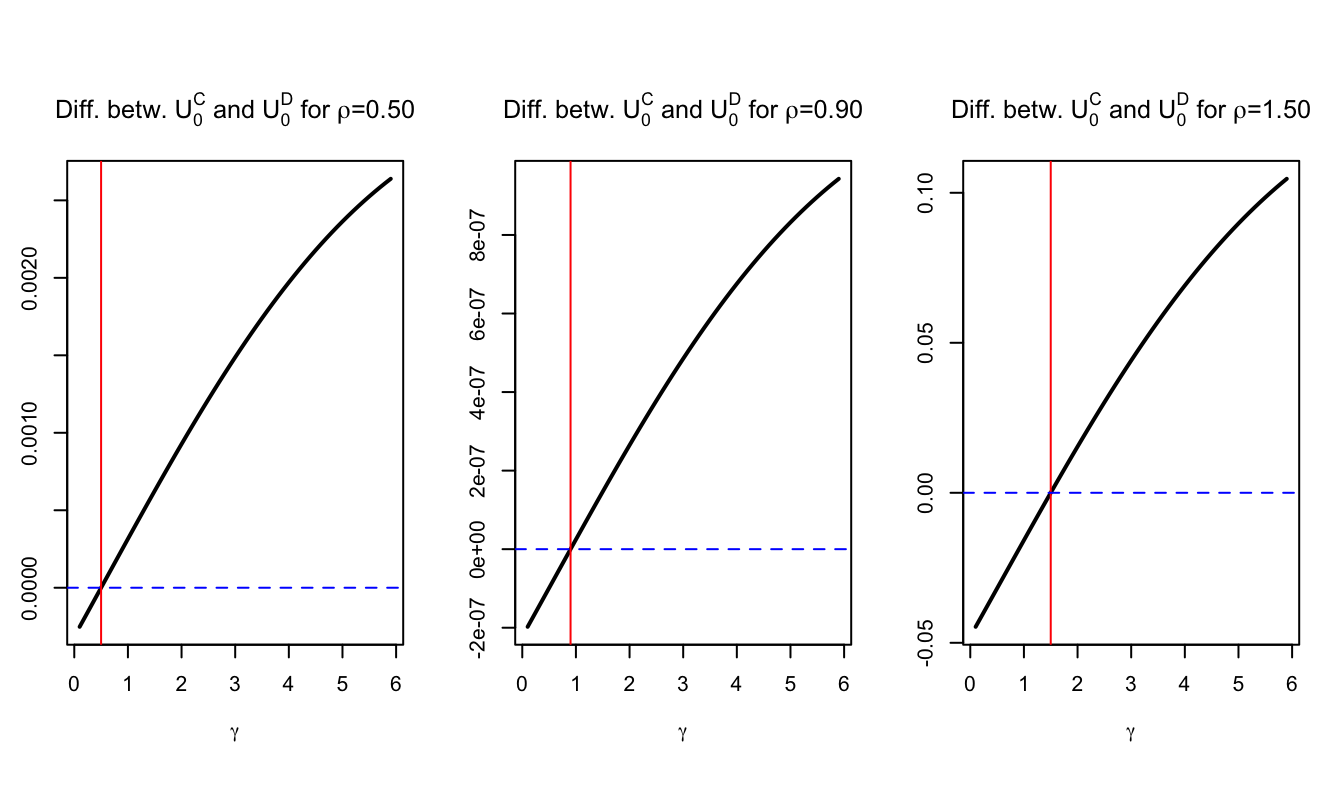
\includegraphics[width=0.95\linewidth]{TSM_files/figure-latex/EZresolution-1} \caption{Comparison of utilities associated with Scenarios C and D. In Scenario C, uncertainty is resolved earlier. Hence, we have a preference for early resolution of uncertainty when the meaasure is positive.}\label{fig:EZresolution}
\end{figure}

\hypertarget{the-sdf-with-epstein-zin-preferences}{%
\subsection{The SDF with Epstein-Zin preferences}\label{the-sdf-with-epstein-zin-preferences}}

Consider an asset that provides the payoff \(x_{t+1}\) at date \(t+1\).
The equilibrium price \(\pi_t(x_{t+1})\) of this asset is such that agents are indifferent between buying or not an additional unit \(\varepsilon\) of this asset.
That is, \(U_t = F(C_t,R_t(U_{t+1}))\) is also equal to:
\begin{eqnarray}
&&  F(C_t,R_t(\color{blue}{U_{t+1}})) \nonumber \\
&=&F(C_t-\varepsilon \pi_t(x_{t+1}),R_t(\color{blue}{F(C_{t+1}+\varepsilon x_{t+1},R_{t+1}(U_{t+2}))})).\label{eq:SDFV}
\end{eqnarray}
Appendix \ref{SDFEZ} shows that this implies that:
\[
\pi_t(x_{t+1}) = \mathbb{E}_t \left( x_{t+1} \mathcal{M}_{t,t+1} \right),
\]
where \(\mathcal{M}_{t,t+1}\), the SDF, is given by:
\begin{equation}
\mathcal{M}_{t,t+1}= \delta \left(\frac{C_{t+1}}{C_t}\right)^{-\rho}  \left(\frac{U_{t+1}}{R_{t}(U_{t+1})}\right)^{\rho-\gamma}.\label{eq:SSS}
\end{equation}

According to \eqref{eq:MRCov}, for all asset \(i\) whose return is \(R_{i,t}\), we have:
\[
\mathbb{E}_t(R_{i,t+1} - R_{f,t}) = - (1 + R_{f,t}) \mathbb{C}ov_t(\mathcal{M}_{t,t+1},R_{i,t+1}).
\]
As a result, under \eqref{eq:SSS}, expected returns depend not only on covariances between returns and consumption growth (as in the C-CAPM) but also on covariances between returns and the next period utility index, which captures news about the investor's future prospects.
To make the formula operational, one has to make the second term more explicit. We will employ the ``wealth portfolio'\,' for that.

Before looking into it, Example \ref{exm:EZpricingInfo} explores an important implication of \eqref{eq:SSS}, namely the fact that, with Epstein-Zin preferences, changes in the information regarding future consumption path is priced---in the sense that it gives rise in specific risk premiums.

\begin{example}[Pricing information on future consumption path]
\protect\hypertarget{exm:EZpricingInfo}{}\label{exm:EZpricingInfo}

Consider the case where \(\rho = 1\) and log-normal conditionally homoskedastic consumption \citep{Cochrane_2005}. Using \(v_t = \log(U_t)\), performing a Taylor expansion of \eqref{eq:EZpreferences} around \(\rho = 1\) leads to:
\begin{equation}
v_t = (1 - \delta) c_t + \delta \frac{1}{1 - \gamma} \log \mathbb{E}_t \left(\exp((1-\gamma)v_{t+1})\right).\label{eq:EZunitIES}
\end{equation}
If \(C_t\) is log-normal, one can show that \(v_t\) is normal. Hence:
\begin{eqnarray}
v_t &=& (1 - \delta) c_t + \delta \mathbb{E}_t(v_{t+1}) + \frac{1}{2}\delta (1-\gamma) \sigma^2(v_{t+1})\nonumber \\
&=& (1 - \delta) \left( \sum_{j=0}^{\infty}  \delta^j \mathbb{E}_t (c_{t+j}) \right) + \frac{1}{2}\delta \frac{1-\gamma}{1-\delta} \sigma^2(v_{t+1}) \label{eq:vrho1}.
\end{eqnarray}
Besides, \eqref{eq:SSS} gives:
\begin{eqnarray*}
m_{t,t+1} &=& \log(\delta) - \rho \Delta c_{t+1} + (\rho - \gamma) \left(v_{t+1} - \frac{1}{1 - \gamma} \log \mathbb{E}_t \left(\exp((1-\gamma)v_{t+1})\right)\right)\\
&=& \log(\delta) - \rho \Delta c_{t+1} + (\rho - \gamma) \left(v_{t+1} - \mathbb{E}_t(v_{t+1}) - \frac{1}{2} \frac{1-\gamma}{1-\delta} \sigma^2(v_{t+1})\right).
\end{eqnarray*}
Using the \emph{``expectation updating'' operator} \(\mathbb{E}_{t+1} - \mathbb{E}_t\), we obtain:
\[
(\mathbb{E}_{t+1} - \mathbb{E}_t) m_{t,t+1} = - \rho(\mathbb{E}_{t+1} - \mathbb{E}_t) c_{t+1} + (\rho - \gamma) (\mathbb{E}_{t+1} - \mathbb{E}_t) v_{t+1},
\]
which gives, when \(\rho = 1\) (using Eq. \eqref{eq:vrho1}):
\begin{eqnarray}
(\mathbb{E}_{t+1} - \mathbb{E}_t) m_{t,t+1} &=& - (\mathbb{E}_{t+1} - \mathbb{E}_t) c_{t+1} +  \\
&& (1 - \gamma)(1 - \delta) (\mathbb{E}_{t+1} - \mathbb{E}_t) \left(  \sum_{j=1}^{\infty}  \delta^j c_{t+j}  \right).\nonumber
\end{eqnarray}

The previous equation can be rewritten as:
\begin{eqnarray}
&& (\mathbb{E}_{t+1} - \mathbb{E}_t) m_{t,t+1} \nonumber \\
&=& - \gamma(\mathbb{E}_{t+1} - \mathbb{E}_t)\Delta c_{t+1} +    (1 - \gamma) \times \underbrace{ (\mathbb{E}_{t+1} - \mathbb{E}_t) \left(  \sum_{j=1}^{\infty}  \delta^j \Delta c_{t+1+j}  \right).}_{\mbox{innov. in long-run cons. growth}}\label{eq:sdfAbc}
\end{eqnarray}
Hence, news about future consumption growth affect the current SDF (marginal rate of substitution). As a consequence, shocks that correlate with updates of future consumption growth are ``priced''. The date-\(t\) prices---and more precisely their risk premium components---depend on the covariances between their payoffs and consumption on date \(t+1\), as well as future consumption growth (regarding \(t+h\), \(h>1\)).

\begin{quote}
If consumption is a random walk, then Epstein-Zin preferences are observationally equivalent to power utility \citep{Kocherlakota_1990}.
\end{quote}

Consider the case where \(C_0 = C_1 = 1\).
At date \(t=1\), one get information about future consumption levels:

\begin{itemize}
\tightlist
\item
  \emph{Case I}: With probability 0.50, one will have \(C_t=\exp(\omega)\) for \(t\ge2\)
\item
  \emph{Case II}: With probability 0.50, one will have \(C_t=\exp(-\omega)\) for \(t\ge2\)
\end{itemize}

where \(\omega \ge 0\).
Eq. \eqref{eq:sdfAbc} implies that:
\[
m_{0,1} = \mathbb{E}_0(m_{0,1}) + (1 - \gamma)\delta \Delta c_{2}.
\]
(using that \(\mathbb{E}_0(\Delta c_{2})=0\) and that \(\mathbb{E}_1(\Delta c_{2})=\Delta c_{2}\).)
Assume that \(\mathbb{E}_0(m_{0,1})\) is such that \(\mathbb{E}_0(\mathcal{M}_{0,1})=\mathbb{E}_0(\exp(m_{0,1}))=1\) (i.e.~the risk-free rate is 0).
We consider the price of an asset that provides 1 at date 1 under Case II and 0 under Case I.
The price of this asset is:
\[
\mathbb{E}_t(\mathcal{M}_{t,t+1}\mathbb{I}_{\{Case II\}}) = \frac{1}{2} \times e^{\mathbb{E}_0(m_{0,1}) - (1 - \gamma)\delta \omega} \times 1.
\]

Figure \ref{fig:EZresolution2} shows the price of this asset for different values of \(\gamma\) and \(\omega\) (\(\delta=0.9\)). With expected utility time-separable preferences (Def. \ref{def:EUTSpref}) the price of such an asset would be 0.50 (represented by the dashed blue line).

\begin{figure}
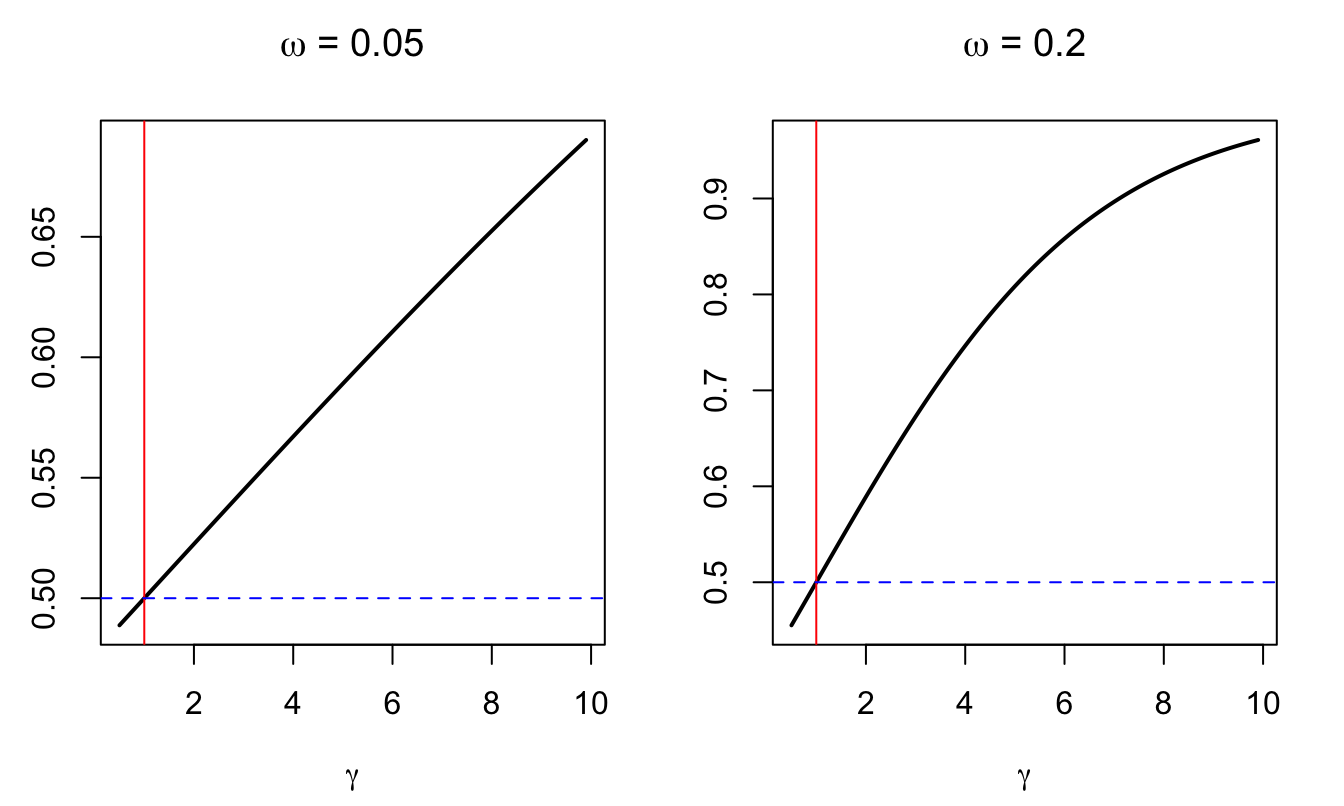
\includegraphics[width=0.95\linewidth]{TSM_files/figure-latex/EZresolution2-1} \caption{Price of an asset that pays 1 under Case II.}\label{fig:EZresolution2}
\end{figure}

\end{example}

Because \(F\) is homogenous of degree one in its arguments (\(C_t\) and \(R_t(U_{t+1})\)), the Euler's theorem yields \citep{HANSEN20073967}:
\begin{equation}
U_t = C_t \frac{\partial U_t}{\partial C_t} +  R_t(U_{t+1}) \frac{\partial U_t}{\partial R_t(U_{t+1})}.\label{eq:XXYXX}
\end{equation}
Taking the current consumption as numeraire, the wealth \(W_t\) is defined by:
\begin{equation}
W_t =   U_t \big/ \frac{\partial U_t}{\partial C_t}.\label{eq:WWWWW}
\end{equation}
It can be understood as a conversion of the intertemporal utility in terms of today's consumption. It can also be seen as a consumption-priced virtual asset that delivers aggregate consumption as its dividends on each time period; this asset is called \emph{wealth portfolio}.\footnote{Since \(F\) homogeneous of order 1, if all future consumption streams are multiplied by \(1+\epsilon\), then the utility becomes \((1+\epsilon)U_t\). Consider the asset that provides \(\epsilon C_{t+h}\) at all future periods (if one purchases \(\epsilon\) units of it). Expressed in consumption units, the equilibrium unit price of this asset (\(\mathcal{W}_t\), say) must satisfy \(-\epsilon U_t + \epsilon \mathcal{W}_t (\partial U_t / \partial C_t)=0\). According to \eqref{eq:WWWWW}, we have \(\mathcal{W}_t = W_t\).}

Using that \(\frac{\partial U_t}{\partial C_t}=(1 - \delta)(V_t^\rho)/(C_t^{\rho})\), we get (using \eqref{eq:WWWWW}):
\begin{equation}
W_t = \frac{U_t^{1-\rho}C_t^\rho}{1 - \delta}.\label{eq:WWW}
\end{equation}
Let's denote by \(R_{a,t+1}\) the return on the wealth portfolio. We have:
\begin{equation}
1+R_{a,t+1} := \frac{W_{t+1}}{W_t - C_t} = \frac{P_{a,t+1}+C_{t+1}}{P_{a,t}},\label{eq:Ra}
\end{equation}
where \(P_{a,t} := W_t - C_t\).

Using \eqref{eq:EZpreferences2} and \eqref{eq:WWW}, it can be shown that:
\[
1+R_{a,t+1} = \left[ \delta \left( \frac{C_{t+1}}{C_t} \right)^{-\rho} \left( \frac{R_t(U_{t+1})}{U_{t+1}} \right)^{1-\rho} \right]^{-1},
\]
which is equivalent to:
\[
\frac{U_{t+1}}{R_t(U_{t+1})} = \left[ \delta (1+ R_{a,t+1}) \left( \frac{C_{t+1}}{C_t} \right)^{-\rho}  \right]^{\frac{1}{1-\rho}}.
\]
Substituting in \eqref{eq:SSS} gives:
\begin{equation}
\mathcal{M}_{t,t+1} =  \delta^{\theta} (1+R_{a,t+1})^{\theta - 1} \left( \frac{C_{t+1}}{C_t} \right)^{- \frac{\theta}{\psi}}
\end{equation}
where
\[
\theta = \frac{1-\gamma}{1-\rho} \quad and \quad \psi = \frac{1}{\rho}.
\]
Therefore (using \(\exp(r_{a,t+1}):=1+R_{a,t+1}\)):
\begin{equation}
\boxed{\log(\mathcal{M}_{t,t+1}) = \theta \log \delta - \frac{\theta}{\psi} \Delta \log(C_{t+1}) - (1-\theta) r_{a,t+1}.}\label{eq:sdfEZ}
\end{equation}

Let's take the log of \eqref{eq:Ra}:
\begin{eqnarray*}
r_{a,t+1} &=& \log(P_{a,t+1}+C_{t+1}) - \log(P_{a,t})\\
&=& z_{t+1} - z_t + g_{t+1} + \log(1 + C_{t+1} / P_{a,t+1}).
\end{eqnarray*}
where \(z_t = \log(P_{a,t}/C_t)\) is the log price-consumption ratio.
Let's denote by \(\bar{z}\) the unconditional mean of \(z_t\). If \(z_t - \bar{z}\) is small, we have:
\begin{eqnarray*}
\log[1 + C_{t+1} / P_{a,t+1}] &=& \log[1 + \exp(-z_{t+1})]\\
&\approx& \log[1 + \exp(-\bar{z})\{1 - (z_{t+1}- \bar{z})\}]\\
&\approx& \log[1 + \exp(-\bar{z}) - \exp(-\bar{z})(z_{t+1}- \bar{z})]\\
&\approx& \log[1 + \exp(-\bar{z})] - \frac{z_{t+1}- \bar{z}}{1 + \exp(\bar{z})}.
\end{eqnarray*}
Therefore:
\begin{equation}
\boxed{r_{a,t+1} \approx \kappa_0 + \kappa_1 z_{t+1} - z_t + g_{t+1},}\label{eq:approxRa}
\end{equation}
where \(\kappa_1= \dfrac{\exp(\bar{z})}{1 + \exp(\bar{z})}\) and \(\kappa_0 = \log(1 + \exp(\bar{z})) + \kappa_1 \bar{z}\).

\begin{quote}
The approximation underlying \eqref{eq:approxRa} is the same as that used by \citet{Campbell_Shiller_1988} used to linearize stock returns.
\end{quote}

For any asset \(i\), whose return is \(1+R_{i,t+1}\), we have:
\begin{equation}
1 = \mathbb{E}_t(\mathcal{M}_{t,t+1}(1+R_{i,t+1})). \quad \mbox{(Euler equation)}\label{eq:Euler}
\end{equation}
The wealth portfolio should also satisfy the Euler equation. That is, for \(1+R_{i,t+1} = 1+R_{a,t+1} = \exp(r_{a,t+1})\), we get:
\begin{equation}
1 = \mathbb{E}_t \left[ \exp\left(\theta \log \delta - \frac{\theta}{\psi} \Delta \log(C_{t+1}) + \theta r_{a,t+1} \right) \right].\label{eq:sdfRa}
\end{equation}

\begin{quote}
The previous equation can be used to calculate an approximately exponential affine SDF. (Indeed, \eqref{eq:sdfEZ} shows that the SDF is approximately exponential affine if \(\Delta \log(C_{t+1})\) and \(r_{a,t+1}\) are affine functions of the state vector.) \citet{Bansal_Yaron_2004} propose the follopwing approach: (a) Conjecture that the log price-consumption ratio \(z_t\) is linear in the sate vector, of the form \(A_0 + A_1'w_t\), say. (b) Then use the fact that the Euler equation has to hold for all values of the state variables to solve for \(A_0\) and \(A_1\).
\end{quote}

\begin{quote}
The same methodology can apply to any asset \(i\). For instance, consider a stock paying dividends \(D_{i,t}\) on each period. The \citet{Campbell_Shiller_1988} approximation implies that \(r_{i,t+1} \approx \kappa_0 + \kappa_1 z_{i,t+1} - z_{i,t} + d_{i,t+1}\) where \(d_{i,t+1}\) is the log-growth rate of dividends and where \(z_{i,t} = \log(P_{i,t}/D_t)\) is the log price-dividend ratio. If \(d_{i,t+1}\) is affine in the state vector, one can then posit that it is also the case of \(z_t= A_{i,0}+A_{i,1}'w_t\), and use the Euler equation
\begin{equation}
1 = \mathbb{E}_t \left[ \exp\left(\theta \log \delta - \frac{\theta}{\psi} \Delta \log(C_{t+1}) - (1 - \theta) r_{a,t+1} + r_{i,t+1} \right) \right].\label{eq:sdfRi}
\end{equation}
to solve for \(A_{i,0}\) and \(A_{i,1}\).
\end{quote}

\hypertarget{long-run-risk-model}{%
\subsection{Long-run risk model}\label{long-run-risk-model}}

We have shown that the CCAPM had difficulties in generating large average excess returns without implying unreasonable risk aversion parameters.
As will be shown later (notably in the \citet{Bansal_Yaron_2004}'s framework), Epstein-Zin preferences can address this problem.
With time-separable utilities, average excess returns (i.e.~risk premiums) had to be accounted by the sole correlation between stock returns and current consumption.
With Epstein-Zin preferences, another key correlation is that between stock returns and updates about future consumption growth---the second term in \eqref{eq:sdfAbc}.
For this second channel to be relevant, observed excess returns should positively correlate to the updates of expectations of long-term consumption. See Figure \ref{fig:SPF10yrStock}.

\begin{figure}
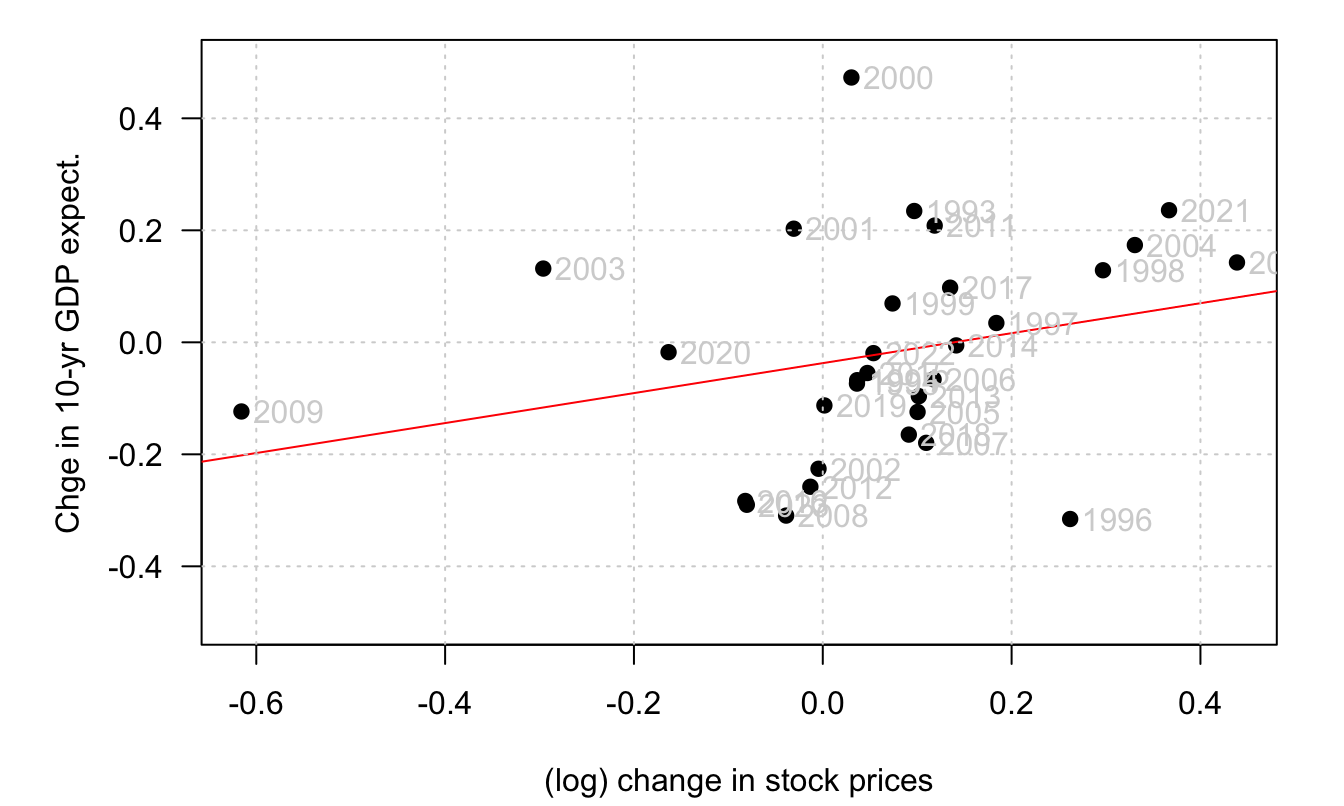
\includegraphics[width=0.95\linewidth]{TSM_files/figure-latex/SPF10yrStock-1} \caption{Sources: SPF Philadelphia and Wilshire 5000 Price Index (FRED database).}\label{fig:SPF10yrStock}
\end{figure}

\citet{Bansal_Yaron_2004} show that the combination of long-run risks and Epstein-Zin preferences allow to address several asset-pricing puzzles. A \href{https://jrenne.shinyapps.io/LRRModels}{web interface} present outputs of the approach. It also allows to simulate the model dynamics and to assess the influence of the parameterization.

In \citet{Bansal_Yaron_2004}'s model, consumption is affected by short-run (high-frequency) and long-run (low frequency) risks. They consider two versions of their model: an homoskedastic one and an heteroskedastic one. In the latter, the conditional variance of consumption moves over time.

\begin{example}[Bansal and Yaron (2004), homoskedastic]
\protect\hypertarget{exm:BYHomsk}{}\label{exm:BYHomsk}

\citet{Bansal_Yaron_2004} postulate the following dynamics for the economy:
\begin{eqnarray*}
x_{t+1} &=& \rho_x x_t + \phi_e \sigma e_{t+1}\\
\Delta c_{t+1} = g_{t+1} &=& \mu + x_t + \sigma \eta_{t+1}\\
g_{d,t+1} &=& \mu_d + \phi x_t + \phi_d \sigma u_{t+1},
\end{eqnarray*}
where \(e_{t+1},\eta_{t+1},u_{t+1} \sim i.i.d. \mathcal{N}(0,1)\). In this model,
\(\mu + x_t\) and \(\mu_d + \phi x_t\) are, respectively, the conditional expectations of consumption growth (\(g_t\)) and dividend growth (\(g_{d,t}\)). Processes \(g_t\) and \(g_{d,t}\) are exogenous. The model is solved by finding associated processes \(r_{a,t}\) and \(r_{m,t}\) that make the model internally consistent. These returns have to satisfy both \eqref{eq:approxRa} and \eqref{eq:sdfRa}.
\(z_t\) and \(z_{m,t}\) are the log price-consumption and price-dividend ratios, respectively, i.e.:
\[
z_t = \log\left(\frac{P_{a,t}}{C_t}\right) \quad and \quad z_{m,t} = \log\left(\frac{P_{m,t}}{C_t}\right).
\]
The price of a claim on aggregate consumption is not observable (return: \(R_{a,t}\)), contrary to the price of the market portfolio (return: \(R_{m,t}\)).

The solution approach is as follows:

\begin{itemize}
\tightlist
\item
  Posit that \(z_t = A_0 + A_1 x_t\);
\item
  substitute the last expression into \eqref{eq:approxRa} and
\item
  inject \(r_{a,t+1}\) in \eqref{eq:sdfRa} and look for the values of \(A_0\) and \(A_1\) that satisfy this Euler equation.
\end{itemize}

Doing the same for \(z_{m,t}\) yields to:
\begin{equation}
A_1 = \frac{1- \dfrac{1}{\psi}}{1 - \kappa_1 \rho_x} \quad and \quad A_{1,m} = \frac{\Phi- \dfrac{1}{\psi}}{1 - \kappa_{1,m} \rho_x}.\label{eq:solABY1}
\end{equation}
If the IES \(\psi > 1\), then \(A_1 > 0\); the price-consumption ratio increases with long-term growth.

\begin{figure}

{\centering 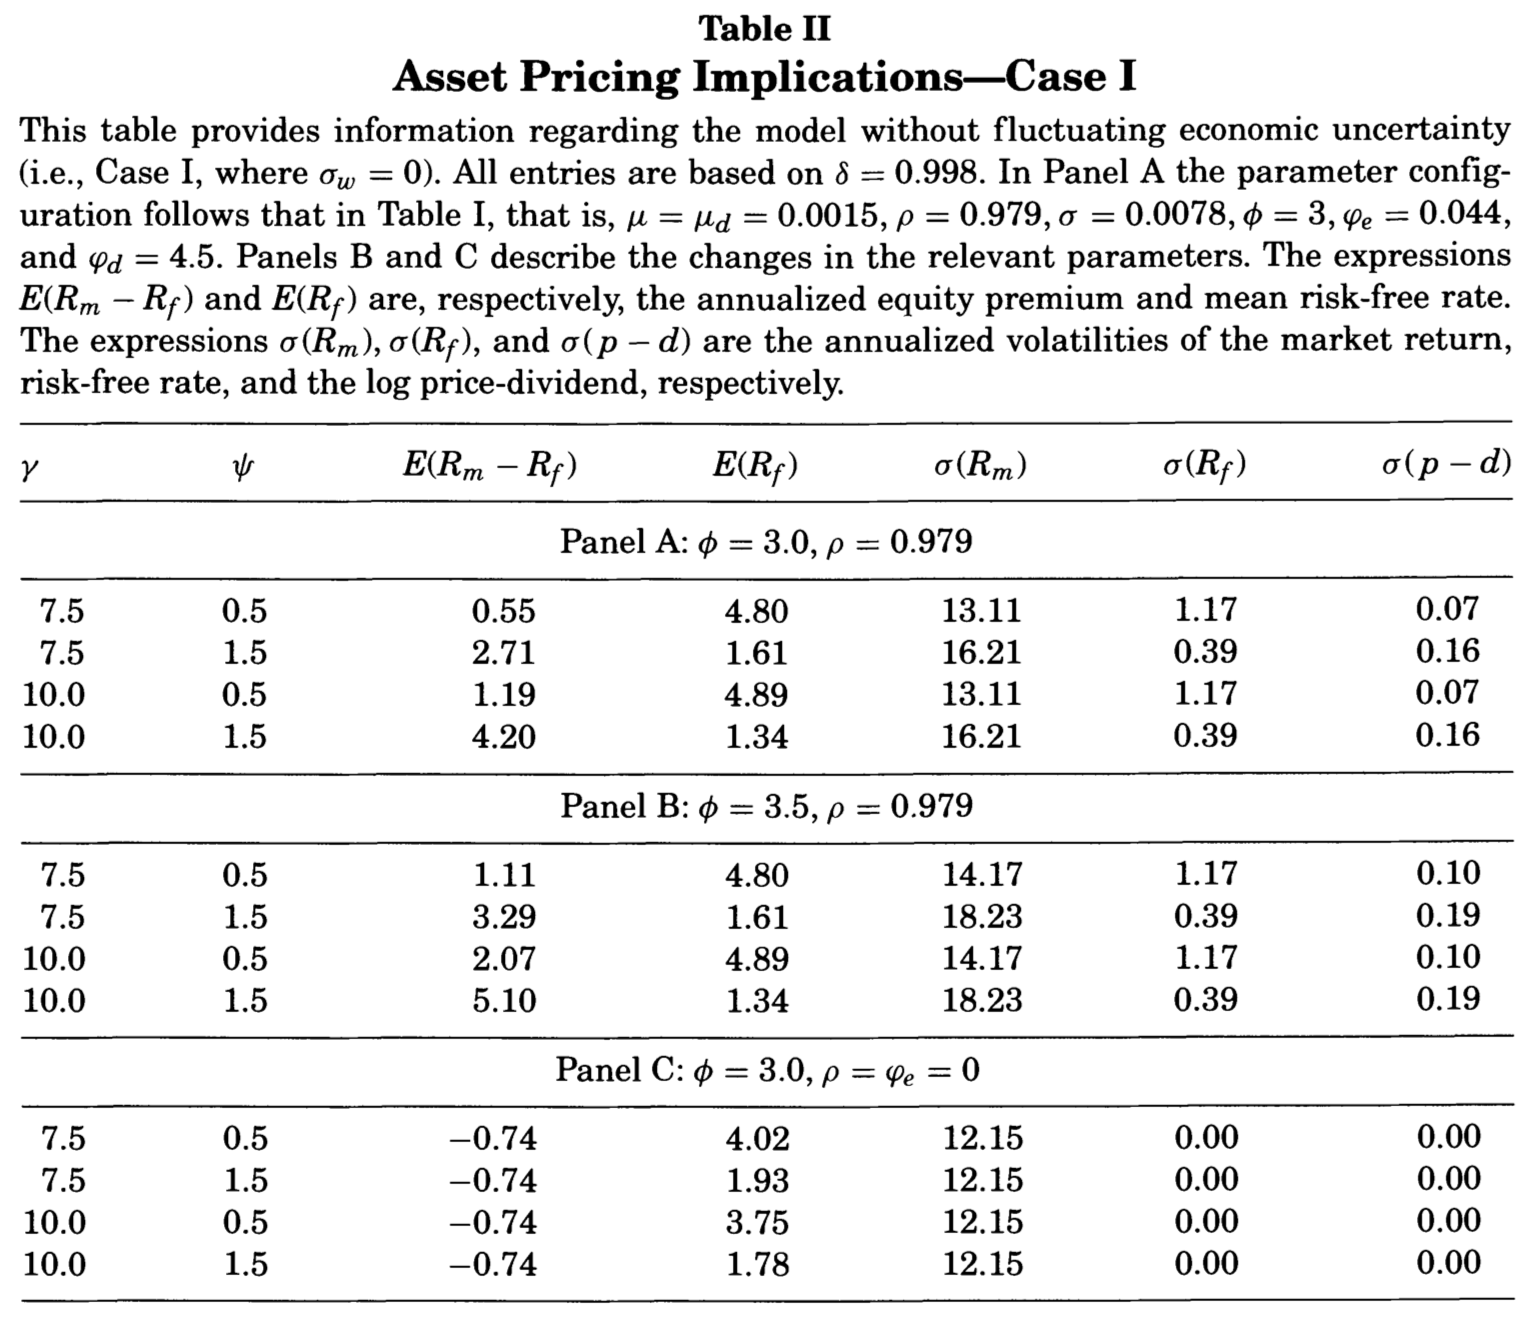
\includegraphics[width=1\linewidth]{figures/table_BY2} 

}

\caption{Source: Bansal and Yaron (2004).}\label{fig:BY2}
\end{figure}

\end{example}

\begin{quote}
\textbf{About the solution procedure}. Eq. \eqref{eq:solABY1} shows that the \(A_i\)s depends on the \(\kappa_i\)s. Eq. \eqref{eq:approxRa} shows that the \(\kappa_i\)s depend on \(\bar{z}\).
Hence, in particular, \(A_0 = f(\bar{z})\). But, in turn, since \(z_t = A_0 + A_1 x_t\), we have \(\bar{z}=A_0 + A_1 \bar{x}=A_0\). For the model to be internally consistent, we should have \(\bar{z}=f(\bar{z})\). Hence, there is a fixed-point problem (\(\bar{z}\) cannot be chosen arbitrarily).
\end{quote}

\begin{quote}
\textbf{The unit EIS case}. Solving for the Epstein-Zin SDF is simpler when the intertemporal elasticity of substitution (EIS) is equal to one \citep{Piazzesi_Schneider_2007}. In that case, and if consumption is an affine combination of affine processes, we can indeed solve for the utility function using \eqref{eq:EZunitIES}. For that: (a) Posit \(v_t = \mu_{v,0}+\mu_{v,1}'w_t\), (b) use the Laplace transform of \(w_t\) in \eqref{eq:EZunitIES} to obtain \(K+1\) restrictions on the scalar \(\mu_{v,0}\) and the vector \(\mu_{v,1}\) (\(K\) is the dimension of \(w_t\)). These restrictions will take the form of non-linear equations (involving the log-Laplace transform of \(w_t\)) that one can solve numerically. (c) Once \(v_t = \mu_{v,0}+\mu_{v,1}'w_t\) is determines, the SDF is obtained from \eqref{eq:SSS}. This strategy is employed, in particular, in \citet{Gourieroux_Monfort_Mouabbi_Renne_2021}, \citet{Monfort_Pegoraro_Renne_Roussellet_2021}, and \citet{Bletzinger_Lemke_Renne_2024}.
\end{quote}

\begin{example}[Bansal and Yaron (2004), heteroskedastic]
\protect\hypertarget{exm:BYHeterosk}{}\label{exm:BYHeterosk}

\citet{Bansal_Yaron_2004} consider a second version of their model. They introduce a novel factor, \(\sigma_t\), that generates time-variation in the conditional variances of consumption and dividends:
\begin{eqnarray}
x_{t+1} &=& \rho_x x_t + \phi_e \sigma_t e_{t+1} \nonumber\\
g_{t+1} &=& \mu + x_t + \sigma_t \eta_{t+1} \nonumber\\
g_{d,t+1} &=& \mu_d + \phi x_t + \phi_d \sigma_t u_{t+1} \nonumber\\
\sigma_{t+1}^2 &=& \sigma^2 + \nu_1(\sigma^2_t -\sigma^2) + \sigma_w w_{t+1}, \label{eq:BYheteroscked}
\end{eqnarray}
where \(e_{t+1},\eta_{t+1},u_{t+1},w_{t+1} \sim i.i.d. \mathcal{N}(0,1)\).
Here, the posited solution for \(z_t\) is:
\[
z_t = A_0 + A_1 x_t + \color{red}{A_2 \sigma^2_t}.
\]
\(A_1\) is unchanged. \(A_2\) is given by (similar form for \(A_{2,m}\)):
\[
A_2 = \frac{0.5 \left[ \left(\theta - \dfrac{\theta}{\psi}\right)^2 + (\theta A_1 \kappa_1 \phi_e)^2 \right]}{\theta(1 - \kappa_1 \nu_1)}.
\]

\begin{figure}

{\centering 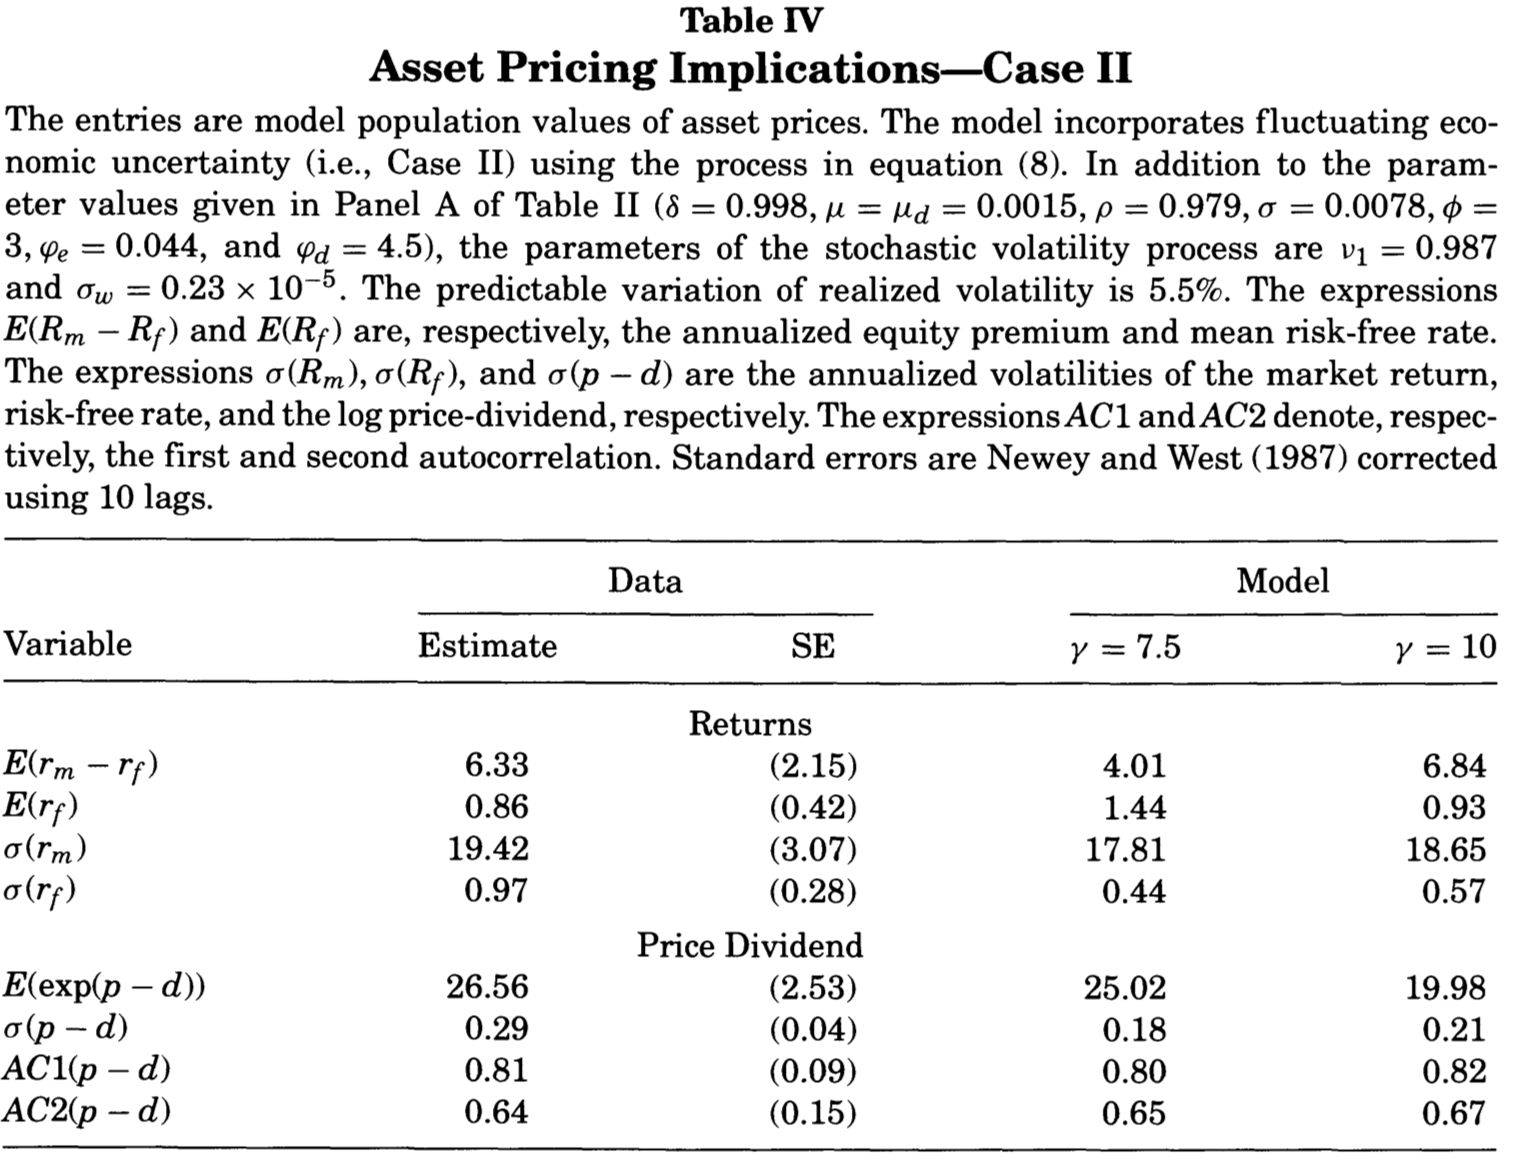
\includegraphics[width=1\linewidth]{figures/table_BY4} 

}

\caption{Source: Bansal and Yaron (2004).}\label{fig:BY4}
\end{figure}

\end{example}

As explained above, together, \eqref{eq:sdfEZ} and \eqref{eq:approxRa} imply an exponential affine SDF. This opens the door to tractable term-structure modeling (see, e.g., Subsection \ref{MHLT} and Section \ref{TSModels}). This is exploited, e.g., by \citet{Bansal_Shaliastovich_2013} (see Example \ref{exm:BS2013}).

\begin{example}[Bansal and Shaliastovich (2013)]
\protect\hypertarget{exm:BS2013}{}\label{exm:BS2013}

\citet{Bansal_Shaliastovich_2013} develop a term structure model where agents feature Epstein-Zin preferences and where the dynamics of macroeconomic takes the form of an heteroskedastic VAR model. Specifically:
\begin{eqnarray*}
\Delta c_{t+1} &=& \mu_c + x_{c,t} + \sigma_c \eta_{c,t+1}\\
\pi_{t+1} &=& \mu_\pi + x_{\pi,t} + \sigma_\pi \eta_{\pi,t+1}\\
\end{eqnarray*}
where \(x_t = [x_{c,t},x_{\pi_t}]'\) follows:
\[
x_t = \left[\begin{array}{cc}\rho_c & \rho_{c \pi}\\0&\rho_\pi\end{array}\right] x_{t-1} + \left[\begin{array}{cc}\sigma_{c,t} & 0\\0&\sigma_{\pi,t}\end{array}\right] e_{t+1},
\]
and
\begin{eqnarray}
\sigma_{c,t+1}^2 &=& (1-\nu_c)\sigma_{xc} + \nu_c\sigma_{c,t}^2  + \sigma_{wc}w_{c,t}\\ \sigma_{\pi,t+1}^2 &=& (1-\nu_\pi)\sigma_{x\pi} + \nu_\pi\sigma_{\pi,t}^2  + \sigma_{w\pi}w_{\pi,t}.
\end{eqnarray}

Functions that allow to handle that type of model are available in package \texttt{EZEqTSM}.\footnote{Use \texttt{install\_github("jrenne/EZEqTSM")}, where \texttt{install\_github} is part of the \texttt{devtools} package.} The following lines of code solve \citet{Bansal_Shaliastovich_2013}'s model and derive the model-implied unconditional yield curves (Figure \ref{fig:BS2013}).

\begin{Shaded}
\begin{Highlighting}[]
\FunctionTok{library}\NormalTok{(EZEqTSM) }\CommentTok{\# loads functions to solve E{-}Z equilibrium models}
\NormalTok{rho.c }\OtherTok{\textless{}{-}} \FloatTok{0.810}\NormalTok{;rho.cpi }\OtherTok{\textless{}{-}} \SpecialCharTok{{-}}\FloatTok{0.047}\NormalTok{;rho.pi }\OtherTok{\textless{}{-}}\NormalTok{ .}\DecValTok{988}
\NormalTok{mu.c }\OtherTok{\textless{}{-}}\NormalTok{ .}\DecValTok{0049}\NormalTok{;mu.pi }\OtherTok{\textless{}{-}}\NormalTok{ .}\DecValTok{009}
\NormalTok{sigma.c  }\OtherTok{\textless{}{-}} \FloatTok{4.6e{-}03}\NormalTok{;sigma.pi }\OtherTok{\textless{}{-}} \FloatTok{5.5e{-}03}
\NormalTok{delta }\OtherTok{\textless{}{-}}\NormalTok{ .}\DecValTok{994}\NormalTok{;gamma }\OtherTok{\textless{}{-}} \FloatTok{20.9}\NormalTok{;psi }\OtherTok{\textless{}{-}} \FloatTok{1.81}
\NormalTok{nu.c  }\OtherTok{\textless{}{-}} \FloatTok{0.994}\NormalTok{;nu.pi }\OtherTok{\textless{}{-}} \FloatTok{0.979}
\NormalTok{sigma.xc  }\OtherTok{\textless{}{-}} \FloatTok{1.09e{-}03}\NormalTok{;sigma.xpi }\OtherTok{\textless{}{-}} \FloatTok{1.11e{-}03}
\NormalTok{sigma.wc  }\OtherTok{\textless{}{-}} \FloatTok{1.85e{-}07}\NormalTok{;sigma.wpi }\OtherTok{\textless{}{-}} \FloatTok{1.81e{-}07}
\NormalTok{freq }\OtherTok{\textless{}{-}} \DecValTok{4} \CommentTok{\# freq is the number of periods per year}
\NormalTok{Model }\OtherTok{\textless{}{-}} \FunctionTok{list}\NormalTok{(}
  \AttributeTok{mu =} \FunctionTok{c}\NormalTok{(mu.c,mu.c,mu.pi),}
  \AttributeTok{Alpha =} \FunctionTok{matrix}\NormalTok{(}\DecValTok{0}\NormalTok{,}\DecValTok{2}\NormalTok{,}\DecValTok{3}\NormalTok{),}
  \AttributeTok{Beta =} \FunctionTok{cbind}\NormalTok{(}\FunctionTok{c}\NormalTok{(}\DecValTok{1}\NormalTok{,}\DecValTok{0}\NormalTok{),}\FunctionTok{c}\NormalTok{(}\DecValTok{1}\NormalTok{,}\DecValTok{0}\NormalTok{),}\FunctionTok{c}\NormalTok{(}\DecValTok{0}\NormalTok{,}\DecValTok{1}\NormalTok{)),}\CommentTok{\# 1st col: beta\_y, 2d: beta\_c, 3rd: beta\_pi}
  \AttributeTok{Omega =} \FunctionTok{matrix}\NormalTok{(}\DecValTok{0}\NormalTok{,}\DecValTok{3}\NormalTok{,}\DecValTok{3}\NormalTok{),}
  \AttributeTok{Pi =} \FunctionTok{matrix}\NormalTok{(}\FunctionTok{c}\NormalTok{(rho.c,}\DecValTok{0}\NormalTok{,rho.cpi,rho.pi),}\DecValTok{2}\NormalTok{,}\DecValTok{2}\NormalTok{),}
  \AttributeTok{chi.0 =} \FunctionTok{c}\NormalTok{(sigma.xc}\SpecialCharTok{\^{}}\DecValTok{2}\NormalTok{,sigma.xpi}\SpecialCharTok{\^{}}\DecValTok{2}\NormalTok{),}
  \AttributeTok{chi.1 =} \FunctionTok{diag}\NormalTok{(}\DecValTok{2}\NormalTok{),}
  \AttributeTok{nu =} \FunctionTok{diag}\NormalTok{(}\FunctionTok{c}\NormalTok{(nu.c,nu.pi)),}
  \AttributeTok{sigma.w =} \FunctionTok{c}\NormalTok{(sigma.wc,sigma.wpi),}
  \AttributeTok{gamma =}\NormalTok{ gamma,}\AttributeTok{delta =}\NormalTok{ delta,}\AttributeTok{psi =}\NormalTok{ psi,}
  \AttributeTok{freq =}\NormalTok{ freq)}
\NormalTok{n }\OtherTok{\textless{}{-}} \FunctionTok{dim}\NormalTok{(Model}\SpecialCharTok{$}\NormalTok{Pi)[}\DecValTok{1}\NormalTok{]}
\NormalTok{q }\OtherTok{\textless{}{-}} \FunctionTok{dim}\NormalTok{(Model}\SpecialCharTok{$}\NormalTok{nu)[}\DecValTok{1}\NormalTok{]}
\NormalTok{Model }\OtherTok{\textless{}{-}} \FunctionTok{solve.model}\NormalTok{(Model) }\CommentTok{\# solve model (i.e. compute SDF)}
\NormalTok{vec.H }\OtherTok{\textless{}{-}} \DecValTok{1}\SpecialCharTok{:}\NormalTok{(Model}\SpecialCharTok{$}\NormalTok{freq }\SpecialCharTok{*} \DecValTok{10}\NormalTok{)}
\NormalTok{W }\OtherTok{\textless{}{-}} \FunctionTok{matrix}\NormalTok{(}\DecValTok{0}\NormalTok{,n}\SpecialCharTok{+}\NormalTok{q}\SpecialCharTok{+}\DecValTok{3}\NormalTok{,}\DecValTok{2}\NormalTok{)}
\NormalTok{W[}\DecValTok{1}\SpecialCharTok{:}\NormalTok{n,}\DecValTok{2}\NormalTok{] }\OtherTok{\textless{}{-}} \SpecialCharTok{+}\NormalTok{Model}\SpecialCharTok{$}\NormalTok{Beta[,}\DecValTok{3}\NormalTok{] }\CommentTok{\# for real bonds}
\NormalTok{W[n}\SpecialCharTok{+}\NormalTok{q}\SpecialCharTok{+}\DecValTok{3}\NormalTok{,}\DecValTok{2}\NormalTok{] }\OtherTok{\textless{}{-}} \SpecialCharTok{+}\DecValTok{1} \CommentTok{\# for real bonds}
\NormalTok{res.price }\OtherTok{\textless{}{-}} \FunctionTok{compute.prices}\NormalTok{(Model,W,vec.H)}
\CommentTok{\# For nominal bonds:}
\NormalTok{eta.}\FloatTok{0.}\NormalTok{nom }\OtherTok{\textless{}{-}}\NormalTok{ res.price}\SpecialCharTok{$}\NormalTok{all.a.return[}\DecValTok{1}\NormalTok{,]}
\CommentTok{\# For real bonds:}
\NormalTok{eta.}\FloatTok{0.}\NormalTok{real }\OtherTok{\textless{}{-}}\NormalTok{ res.price}\SpecialCharTok{$}\NormalTok{all.a.return[}\DecValTok{2}\NormalTok{,] }\SpecialCharTok{{-}}\NormalTok{ Model}\SpecialCharTok{$}\NormalTok{mu[}\DecValTok{3}\NormalTok{]}
\FunctionTok{par}\NormalTok{(}\AttributeTok{mfrow=}\FunctionTok{c}\NormalTok{(}\DecValTok{1}\NormalTok{,}\DecValTok{1}\NormalTok{));}\FunctionTok{par}\NormalTok{(}\AttributeTok{plt=}\FunctionTok{c}\NormalTok{(.}\DecValTok{15}\NormalTok{,.}\DecValTok{95}\NormalTok{,.}\DecValTok{2}\NormalTok{,.}\DecValTok{95}\NormalTok{))}
\FunctionTok{plot}\NormalTok{(freq}\SpecialCharTok{*}\NormalTok{eta.}\FloatTok{0.}\NormalTok{nom,}\AttributeTok{type=}\StringTok{"l"}\NormalTok{,}\AttributeTok{lwd=}\DecValTok{2}\NormalTok{,}\AttributeTok{ylim=}\FunctionTok{c}\NormalTok{(}\DecValTok{0}\NormalTok{,freq}\SpecialCharTok{*}\FunctionTok{max}\NormalTok{(eta.}\FloatTok{0.}\NormalTok{nom)),}
     \AttributeTok{las=}\DecValTok{1}\NormalTok{,}\AttributeTok{xlab=}\StringTok{"maturity"}\NormalTok{,}\AttributeTok{ylab =} \StringTok{"rates"}\NormalTok{,}\AttributeTok{las=}\DecValTok{1}\NormalTok{);}\FunctionTok{grid}\NormalTok{()}
\FunctionTok{lines}\NormalTok{(freq}\SpecialCharTok{*}\NormalTok{eta.}\FloatTok{0.}\NormalTok{real,}\AttributeTok{lwd=}\DecValTok{2}\NormalTok{,}\AttributeTok{lty=}\DecValTok{3}\NormalTok{)}
\end{Highlighting}
\end{Shaded}

\begin{figure}
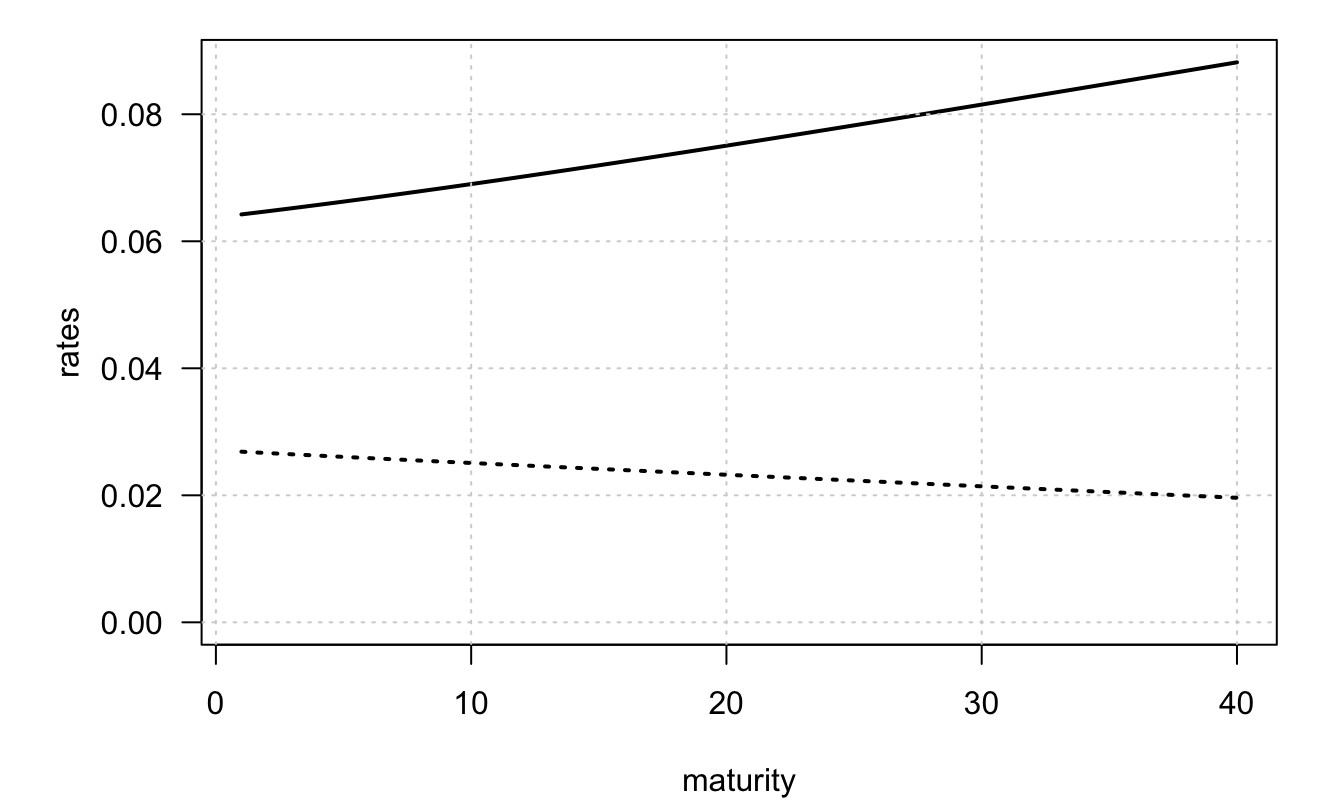
\includegraphics[width=0.95\linewidth]{TSM_files/figure-latex/BS2013-1} \caption{Unconditional yield curves in Bansal and Shaliastovich (2013). The solid line (respectively dotted line) is the unconditional nominal (resp. real) yield curve.}\label{fig:BS2013}
\end{figure}

\end{example}

Figure \ref{fig:BS2013} shows that the unconditional real yield curve is downward-sloping in \citet{Bansal_Shaliastovich_2013}, which is a standard result of the equilibrium term-structure model literature \citep{Piazzesi_Schneider_2007}. As explained in \citet{Bletzinger_Lemke_Renne_2024}, this results from the fact that equilibrium term-structure models usually mode the consumption process by focusing on its growth rate, which they take to be persistent (AR processes, or sums of AR processes). Since, in equilibrium models, real rates depend on expected consumption growth, this mechanically implies that real rates are low in bad states of the world. \citet{Bletzinger_Lemke_Renne_2024} show that this effect is alleviated when one introduces a trend-cycle modeling of consumption.

The term structure of nominal rates is upward-sloping because \(\rho_{c\pi}<0\) generates a negative correlation between inflation and consumption growth. In such an environment, nominal bonds experience a decline in value during recessions, making them ineffective as hedging instruments. Consequently, investors choose to hold these bonds only if their returns, on average, exceed those obtained from rolling over a portfolio invested in short-term bonds. (Hence, the positive nominal term premiums.) Conversely, when \$\rho\_\{c\pi\}\textgreater0,'' the argument reverses, and the average nominal yield curve would exhibit a downward-sloping pattern.

\hypertarget{PHabitat}{%
\section{Preferred-habitat model of the term-structure of interest rate}\label{PHabitat}}

A very different type of asset-pricing structural model has been introduced by \citet{Greenwood_Vayanos_2014} and \citet{Vayanos_Vila_2021}. In the present section, we derive the approximate yield curve solution to this type of model in discrete-time (while the original model is written in continuous time); this derivations is broadly based on \citet{Hamilton_Wu_2012} and \citet{Hayashi_2018}.

Term structure models based on preferred habitat theory are a class of financial models that extend traditional yield curve models by incorporating the notion that some investors or issuers exhibit preferences for specific maturity segments, or ``habitats,'' in the bond market. These models provide a nuanced understanding of how market participants' varying preferences for maturity segments influence interest rates and the overall shape of the yield curve.

In these models, there are two broad categories of market participants: the preferred-habitant investors/issuers and the arbitrageurs. The latter have no preferred habitat, they aim to maximize their wealth under risk constraints.

Denote by \(P_{n,t}\) the date-\(t\) prices of a \(n\)-period conventional zero-coupon bonds, and by \(N\) the maximum bond maturity. Arbitrageurs' wealth evolves according to:
\[
W_{t+1} = \left(\sum_{n=1}^N z_{n,t}\frac{P_{n-1,t+1}}{P_{n,t}}\right)W_t,
\]
where \(z_{n,t}\) is the fraction of wealth invested in \(n\)-period bonds on date \(t\). The portfolio's return between dates \(t\) and \(t+1\) is:
\begin{eqnarray*}
r_{t,t+1} &=& \frac{W_{t+1}-W_t}{W_t}=
\sum_{n=1}^N z_{n,t}\left(\frac{P_{n-1,t+1}}{P_{n,t}}-1\right) = \sum_{n=1}^N z_{n,t}r_{n,t,t+1},
\end{eqnarray*}
where \(r_{n,t,t+1}\) is the one-period return of the \(n\)-period bond.

\begin{hypothesis}
\protect\hypertarget{hyp:prefArbit}{}\label{hyp:prefArbit}On date \(t\), arbitrageurs determine \(z_t=[z_{1,t},\dots,z_{N,t}]'\) so as to maximize:
\[
\mathbb{E}_t(r_{t,t+1}) - \frac{\gamma}{2}\mathbb{V}ar_t(r_{t,t+1}),
\]
under the constraint that \(\sum_n^N z_{n,t} = 1\).
\end{hypothesis}

\begin{hypothesis}
\protect\hypertarget{hyp:dynF}{}\label{hyp:dynF}The state of the economy is characterized by a \(m\)-dimensional vector of factors, denoted \(f_t\), which follows a Gaussian vector auto-regressive process of order one:
\[
f_t = \mu_f + \Phi f_{t-1} + \Sigma \varepsilon_t,
\]
with \(\varepsilon_t \sim\,i.i.d.\,\mathcal{N}(0,Id)\).
\end{hypothesis}

Let us denote by \(y_{n,t}\) the yield-to-maturity of a \(n\)-period zero-coupon bond. We have:
\begin{equation}
i_{n,t} = - \frac{1}{n}\log P_{n,t}.\label{eq:Pandy}
\end{equation}

\begin{proposition}[Bond prices]
\protect\hypertarget{prp:prop111}{}\label{prp:prop111}Under Assumptions \ref{hyp:prefArbit} and \ref{hyp:dynF}, and if the prices of \(n\)-period zero-coupon bonds are given by exponential affine functions of \(f_t\), that is, if
\begin{equation}
P_{n,t} = \exp(a_{n,t} + b_{n,t}'f_t), \label{eq:PPs}    
\end{equation}
(which implies, in particular, that we must have \(i_{1,t} = - a_1 - b_1'f_t\)), then \(a_n\) and \(b_n\) approximately verify, for \(n \ge 2\):
\begin{eqnarray}
-a_1-b_1' f_t &\approx& a_{n-1} + b_{n-1}'\mu_f  - a_{n} + b_{n-1}'\Phi f_t - b_{n}'f_{t} + \nonumber \\ &&\frac{1}{2}b_{n-1}'\Sigma \Sigma'b_{n-1} - \gamma b_{n-1}'\Sigma\Sigma'\Theta' z_t, \label{eq:Lagr1B}
\end{eqnarray}
where \(\Theta\) is an \(N \times m\) matrices whose \(n^{th}\) rows is \(b_{n-1}'\). (Note that the first rows of this matrix is filled with zeros.)
\end{proposition}

\begin{proof}
Using that \(z_{1,t} = 1 - \sum_{n=2}^{N}z_{n,t}\), and noting that \(i_{1,t}=r_{1,t,t+1}\), one obtains the following first-order conditions to the arbitrageurs' problem (as defined by Assumption \ref{hyp:prefArbit}), for \(n \ge 2\):
\begin{eqnarray}
i_{1,t} &=& \mathbb{E}_t(r_{n,t,t+1}) - \frac{\gamma}{2} \frac{\partial}{\partial z_{n,t}} \mathbb{V}ar_t(r_{t,t+1}). \label{eq:Lagr1}
\end{eqnarray}
When bond prices are as in \eqref{eq:PPs}, we have:
\begin{eqnarray*}
r_{n,t,t+1} &=& P_{n-1,t+1}/P_{n,t}-1 = \exp(a_{n-1} + b_{n-1}'f_{t+1} - a_{n} - b_{n}'f_{t})-1,
\end{eqnarray*}
from which we get the following approximations, assuming that one-period bond returns are small \citep{Hamilton_Wu_2012}:
\begin{eqnarray}
\mathbb{E}_t(r_{n,t,t+1}) &\approx&  a_{n-1} + b_{n-1}'\mu_f  - a_{n} + b_{n-1}'\Phi f_t - b_{n}'f_{t}\nonumber\\
&&+ \frac{1}{2}b_{n-1}'\Sigma \Sigma'b_{n-1}. \label{eq:Exp1}
\end{eqnarray}
Moreover, using \(r_{n,t,t+1} \approx \log(P_{n-1,t+1}/P_{n,t})\), we get:
\begin{equation}
\mathbb{V}ar_t(r_{t,t+1}) \approx z_t'\Theta\Sigma\Sigma'\Theta' z_t.\label{eq:Var}
\end{equation}
Eq. \eqref{eq:Var} implies in particular that:
\begin{eqnarray*}
\frac{\partial}{\partial z_t} \mathbb{V}ar_t(r_{t,t+1}) &\approx& 2 \Theta\Sigma\Sigma'\Theta' z_t,
\end{eqnarray*}
which, in turn, gives:
\begin{eqnarray*}
\frac{\partial}{\partial z_{n,t}} \mathbb{V}ar_t(r_{t,t+1}) &\approx& 2 b_{n-1}'\Sigma\Sigma'\Theta' z_t.
\end{eqnarray*}
Using the previous equation as well as \eqref{eq:Exp1} in \eqref{eq:Lagr1} leads to \eqref{eq:Lagr1B}.
\end{proof}

\begin{hypothesis}[Bond supply]
\protect\hypertarget{hyp:supply}{}\label{hyp:supply}Bond supplies, expressed as fractions of the arbitrageurs' wealth, depend on a time-varying component (\(\alpha_n + \beta_n' f_t\)) and on yields-to-maturity. Specifically:
\begin{eqnarray}
s_{n,t} &=& (\alpha_n + {\beta_n}' f_t) - \zeta_n i_{n,t}. \label{eq:supply1}
\end{eqnarray}
\end{hypothesis}

\begin{definition}[Equilibrium]
\protect\hypertarget{def:Equilib}{}\label{def:Equilib}In equilibrium, bond market clears (for each maturity). Arbitrageurs maximize the problem defined in Assumption \ref{hyp:prefArbit}, which determines the bond demand, and bond supply is determined by Assumption \ref{hyp:supply}.
\end{definition}

\begin{proposition}[Bond prices]
\protect\hypertarget{prp:PropII}{}\label{prp:PropII}Under Assumptions \ref{hyp:prefArbit} to \ref{hyp:supply}, and if bond prices are exponential affine in \(f_t\), then the loadings \(a_n\) and \(b_n\)---which appear in equation \eqref{eq:PPs}---approximately satisfy the following recursive equations, for \(n\ge 1\):
\begin{equation}
\left\{
\begin{array}{cll}
a_n &\approx& a_1 + a_{n-1} + b_{n-1}'\mu_f^{\mathbb{Q}} + \frac{1}{2}b_{n-1}'\Sigma \Sigma'b_{n-1} \\
b_n &\approx& b_1 + {\Phi^{\mathbb{Q}}}'b_{n-1},
\end{array}
\right.\label{eq:recursConventio}
\end{equation}
with \(a_0=0\), \(b_0=0\), and where
\begin{equation}
\mu_f^{\mathbb{Q}} = \mu_f - \Sigma \lambda \quad \mbox{and} \quad \Phi^{\mathbb{Q}} = \Phi - \Sigma \Lambda,\label{eq:muPHIQ}
\end{equation}
with
\begin{equation}
\lambda = \gamma \Sigma' \Theta'\mathcal{A} \quad \mbox{and} \quad \Lambda = \gamma \Sigma' \Theta'\mathcal{B},\label{eq:lambdas} 
\end{equation}
\(\mathcal{A}\) being a \(N\)-dimensional vector whose \(n^{th}\) entry is \(\alpha_n + \frac{1}{n}\zeta_n a_n\), and \(\mathcal{B}\) being a \(N \times m\) matrix whose \(n^{th}\) row is \((\beta_n + \frac{1}{n}\zeta_n b_n)'\). (Matrix \(\Theta\) is defined in Proposition \ref{prp:prop111}.)
\end{proposition}

\begin{proof}
If prices are as in \eqref{eq:PPs}, and using \eqref{eq:Pandy}, we have:
\[
i_{n,t} = -\frac{1}{n}(a_n + b_n'f_t).
\]

Combining the last equation with \eqref{eq:supply1} gives:
\begin{eqnarray}
s_{n,t} &=& \alpha_n  + \frac{1}{n}\zeta_n a_n + \left(\beta_n + \frac{1}{n}\zeta_n b_n\right)'f_t.
\end{eqnarray}
At equilibrium, we have \(z_{n,t}=s_{n,t}\), which imples that the \(z_t\)'s are affine functions of \(f_t\). Specifically, we have:
\[
z_t = \mathcal{A} + \mathcal{B}f_t.
\]
This implies that we have:
\[
\gamma \Sigma' B'z_t  = \lambda + \Lambda f_t,
\]
with \(\lambda\) and \(\Lambda\) given in \eqref{eq:lambdas}. Using these notations, \eqref{eq:Lagr1B} rewrites:
\begin{eqnarray*}
i_{1,t} &\approx& a_{n-1} + b_{n-1}'\mu_f  - a_{n} + b_{n-1}'\Phi f_t - b_{n}'f_{t} + \frac{1}{2}b_{n-1}'\Sigma \Sigma'b_{n-1} - b_{n-1}'\Sigma (\lambda + \Lambda f_t).
\end{eqnarray*}
Using the notations introduced in \eqref{eq:muPHIQ}, this leads to:
\begin{eqnarray}
&&- a_1 - b_1' f_t \nonumber\\
&\approx& a_{n-1} + b_{n-1}'\mu_f^{\mathbb{Q}}  - a_{n} + b_{n-1}'\Phi^{\mathbb{Q}} f_t - b_{n}'f_{t} + \frac{1}{2}b_{n-1}'\Sigma \Sigma'b_{n-1}. \label{eq:Lagr1C}
\end{eqnarray}
The recursions \eqref{eq:recursConventio} are required for \eqref{eq:Lagr1C} to be satisfied for any value of \(f_t\).
\end{proof}

\begin{quote}
The first row of \(\Theta\) is \(b_0'=0\). As a result, looking at \eqref{eq:lambdas}, it appears that the first component entry of \(\mathcal{A}\) (namely \(\alpha_1 + \zeta_1 a_1\)) and the first row of \(\mathcal{B}\) (namely \(\beta_1' + \zeta_1 b_1'\)) do not appear in \(\lambda\), nor in \(\Lambda\). This gives the impression that the bond supply specification for one-period bond has no pricing impact. This is however false, as we must have:
\[
\sum_{n=1}^N z_{i,t} = 1.
\]
For this to hold for any value of \(f_t\), we need to have (using \(z_t = \mathcal{A} + \mathcal{B}f_t\)):
\begin{eqnarray}
\alpha_1 + \zeta_1 a_1 &=& 1 - \sum_{n=2}^N\mathcal{A}_i \label{eq:constr1}\\
\beta_1 + \zeta_1 b_1&=&  - \sum_{n=2}^N\mathcal{B}_i,\label{eq:constr2}
\end{eqnarray}
where \(\mathcal{B}_i\) is the \(i^{th}\) row of \(\mathcal{B}\). These two equations show that \(a_1\) and \(b_1\) cannot be chosen independently from the specification of the supply for one-period bonds (characterized by \(\alpha_1\), \(\beta_1\), and \(\zeta_1\)).
In particular, consider the case where one factor corresponds to the conventional short-term yield (a situation that is standard in the literature). Assume for instance that the first component of \(f_t\) is the conventional one-period yield. In that case, we have:
\[
a_1 = 0 \quad \mbox{and}\quad b_1 = [-1,0,0,\dots]'.
\]
Assume that \eqref{eq:supply1} holds for \(n \ge 2\). Proposition \ref{prp:PropII} then states that one can solve for the \((a_n,b_n)\)'s. However, it should then by checked that \(\alpha_1\), \(\beta_1\), and \(\zeta_1\) satisfy \eqref{eq:constr1} and \eqref{eq:constr2}. Alternatively, assuming for instance that \(\zeta_1\) is fixed, one can deduce \(\alpha_1\) and \(\beta_1\).
\end{quote}

The following lines of codes build a discrete-time version of the model proposed by \citet{Vayanos_Vila_2021}. This model features two factors. The first (\(f_{1,t}\)) is the short-term interest rate, the seconf (\(f_{2,t}\)) is a supply factor. Parameters \(\zeta_n\), \(\alpha_n\), and \(\beta_{n,2}\), defining the specification of bond supplies (see Assumption \ref{hyp:supply}, are given by:\footnote{We have \(\beta_{n,1}=0\) for all \(n \ge 1\). That is, the short-term rate has no direct influence on the \(s_{n,t}\)'s.}
\begin{eqnarray}
\zeta_n &=& \zeta_0 n \exp(-\delta_\zeta n) \\
\beta_{n,2} &=& \kappa_{\beta} \big( \exp(-\delta_\zeta n) - \exp(-\delta_{\beta} n) \big) \\
\alpha_n &=& \kappa_\alpha \big( \exp(-\delta_\zeta n) - \exp(-\delta_{\beta,1} n) \big) \end{eqnarray}

Figure \ref{fig:VV1} shows the influence of the latter on bond supply (the \(s_{n,t}\)'s). Note that the figure shows only the \(\beta_{n,2}\)'s for \(n \ge 2\), since \(\beta_{1,2}\) is residual of the model solution.

\begin{Shaded}
\begin{Highlighting}[]
\FunctionTok{library}\NormalTok{(TSModels)}
\NormalTok{m }\OtherTok{\textless{}{-}} \DecValTok{2} \CommentTok{\# number of factors}
\NormalTok{N }\OtherTok{\textless{}{-}} \DecValTok{30} \CommentTok{\# maximum maturity}
\CommentTok{\# Calibration: see Table 1 in Vayanos{-}Vila:}
\NormalTok{kappa\_r }\OtherTok{\textless{}{-}}\NormalTok{ .}\DecValTok{125}\NormalTok{;sigma\_r }\OtherTok{\textless{}{-}}\NormalTok{ .}\DecValTok{0146}
\NormalTok{kappa\_beta }\OtherTok{\textless{}{-}}\NormalTok{ .}\DecValTok{053}\NormalTok{;a.theta }\OtherTok{\textless{}{-}} \DecValTok{3155}
\NormalTok{a.alpha }\OtherTok{\textless{}{-}} \FloatTok{35.3}\NormalTok{; delta\_alpha }\OtherTok{\textless{}{-}}\NormalTok{ .}\DecValTok{297}
\NormalTok{delta\_theta }\OtherTok{\textless{}{-}}\NormalTok{ .}\DecValTok{307}\NormalTok{;alpha }\OtherTok{\textless{}{-}} \FloatTok{5.21}\NormalTok{;r\_bar }\OtherTok{\textless{}{-}} \FloatTok{4.8}\NormalTok{;a.theta0 }\OtherTok{\textless{}{-}} \DecValTok{289}
\CommentTok{\# Specif of minus short{-}rate:}
\NormalTok{a1 }\OtherTok{\textless{}{-}} \SpecialCharTok{{-}}\NormalTok{ r\_bar}\SpecialCharTok{/}\DecValTok{100} \CommentTok{\# minus mean of short{-}term rate}
\NormalTok{b1 }\OtherTok{\textless{}{-}} \FunctionTok{matrix}\NormalTok{(}\FunctionTok{c}\NormalTok{(}\SpecialCharTok{{-}}\DecValTok{1}\NormalTok{,}\FunctionTok{rep}\NormalTok{(}\DecValTok{0}\NormalTok{,m}\DecValTok{{-}1}\NormalTok{)),}\AttributeTok{ncol=}\DecValTok{1}\NormalTok{) }\CommentTok{\# The first factor is r\_t}
\CommentTok{\# Specify factors\textquotesingle{} dynamics:}
\NormalTok{mu\_f  }\OtherTok{\textless{}{-}} \FunctionTok{matrix}\NormalTok{(}\DecValTok{0}\NormalTok{,m,}\DecValTok{1}\NormalTok{)}
\NormalTok{Phi   }\OtherTok{\textless{}{-}} \FunctionTok{diag}\NormalTok{(}\FunctionTok{c}\NormalTok{(}\DecValTok{1}\SpecialCharTok{{-}}\NormalTok{kappa\_r,}\DecValTok{1}\SpecialCharTok{{-}}\NormalTok{kappa\_beta))}
\NormalTok{Sigma }\OtherTok{\textless{}{-}} \FunctionTok{diag}\NormalTok{(}\FunctionTok{c}\NormalTok{(sigma\_r,sigma\_r))}
\CommentTok{\# Specify supply of bonds:}
\NormalTok{a }\OtherTok{\textless{}{-}}\NormalTok{ a.alpha}\SpecialCharTok{/}\NormalTok{alpha;theta }\OtherTok{\textless{}{-}}\NormalTok{ a.theta}\SpecialCharTok{/}\NormalTok{a; theta0 }\OtherTok{\textless{}{-}}\NormalTok{ a.theta0}\SpecialCharTok{/}\NormalTok{a}
\NormalTok{Alpha      }\OtherTok{\textless{}{-}} \FunctionTok{matrix}\NormalTok{(theta0 }\SpecialCharTok{*}\NormalTok{ (}\FunctionTok{exp}\NormalTok{(}\SpecialCharTok{{-}}\NormalTok{delta\_alpha}\SpecialCharTok{*}\NormalTok{(}\DecValTok{1}\SpecialCharTok{:}\NormalTok{N)) }\SpecialCharTok{{-}}
                                 \FunctionTok{exp}\NormalTok{(}\SpecialCharTok{{-}}\NormalTok{delta\_theta}\SpecialCharTok{*}\NormalTok{(}\DecValTok{1}\SpecialCharTok{:}\NormalTok{N))),N,}\DecValTok{1}\NormalTok{)}
\NormalTok{Beta      }\OtherTok{\textless{}{-}} \FunctionTok{matrix}\NormalTok{(}\DecValTok{0}\NormalTok{,N,m)}
\NormalTok{Beta[,}\DecValTok{2}\NormalTok{]  }\OtherTok{\textless{}{-}}\NormalTok{ theta }\SpecialCharTok{*}\NormalTok{ (}\FunctionTok{exp}\NormalTok{(}\SpecialCharTok{{-}}\NormalTok{delta\_alpha}\SpecialCharTok{*}\NormalTok{(}\DecValTok{1}\SpecialCharTok{:}\NormalTok{N)) }\SpecialCharTok{{-}}
                        \FunctionTok{exp}\NormalTok{(}\SpecialCharTok{{-}}\NormalTok{delta\_theta}\SpecialCharTok{*}\NormalTok{(}\DecValTok{1}\SpecialCharTok{:}\NormalTok{N)))}
\NormalTok{Zeta      }\OtherTok{\textless{}{-}}\NormalTok{ alpha }\SpecialCharTok{*} \FunctionTok{matrix}\NormalTok{(}\DecValTok{1}\SpecialCharTok{:}\NormalTok{N }\SpecialCharTok{*} \FunctionTok{exp}\NormalTok{(}\SpecialCharTok{{-}}\NormalTok{delta\_alpha}\SpecialCharTok{*}\NormalTok{(}\DecValTok{1}\SpecialCharTok{:}\NormalTok{N)),N,}\DecValTok{1}\NormalTok{)}
\NormalTok{model }\OtherTok{\textless{}{-}} \FunctionTok{list}\NormalTok{(}\AttributeTok{gamma =}\NormalTok{ a,}\AttributeTok{mu\_f =}\NormalTok{ mu\_f,}\AttributeTok{Phi =}\NormalTok{ Phi,}\AttributeTok{Sigma =}\NormalTok{ Sigma,}
              \AttributeTok{Alpha =}\NormalTok{ Alpha,}\AttributeTok{Beta =}\NormalTok{ Beta,}\AttributeTok{Zeta =}\NormalTok{ Zeta,}\AttributeTok{a1 =}\NormalTok{ a1,}\AttributeTok{b1 =}\NormalTok{ b1)}
\FunctionTok{plot}\NormalTok{(}\DecValTok{2}\SpecialCharTok{:}\NormalTok{N,Beta[}\DecValTok{2}\SpecialCharTok{:}\NormalTok{N,}\DecValTok{2}\NormalTok{],}\AttributeTok{type=}\StringTok{"l"}\NormalTok{,}\AttributeTok{lwd=}\DecValTok{2}\NormalTok{,}\AttributeTok{xlab=}\StringTok{"maturity"}\NormalTok{,}\AttributeTok{ylab=}\StringTok{""}\NormalTok{)}
\FunctionTok{abline}\NormalTok{(}\AttributeTok{h=}\DecValTok{0}\NormalTok{,}\AttributeTok{col=}\StringTok{"grey"}\NormalTok{,}\AttributeTok{lty=}\DecValTok{3}\NormalTok{)}
\end{Highlighting}
\end{Shaded}

\begin{figure}
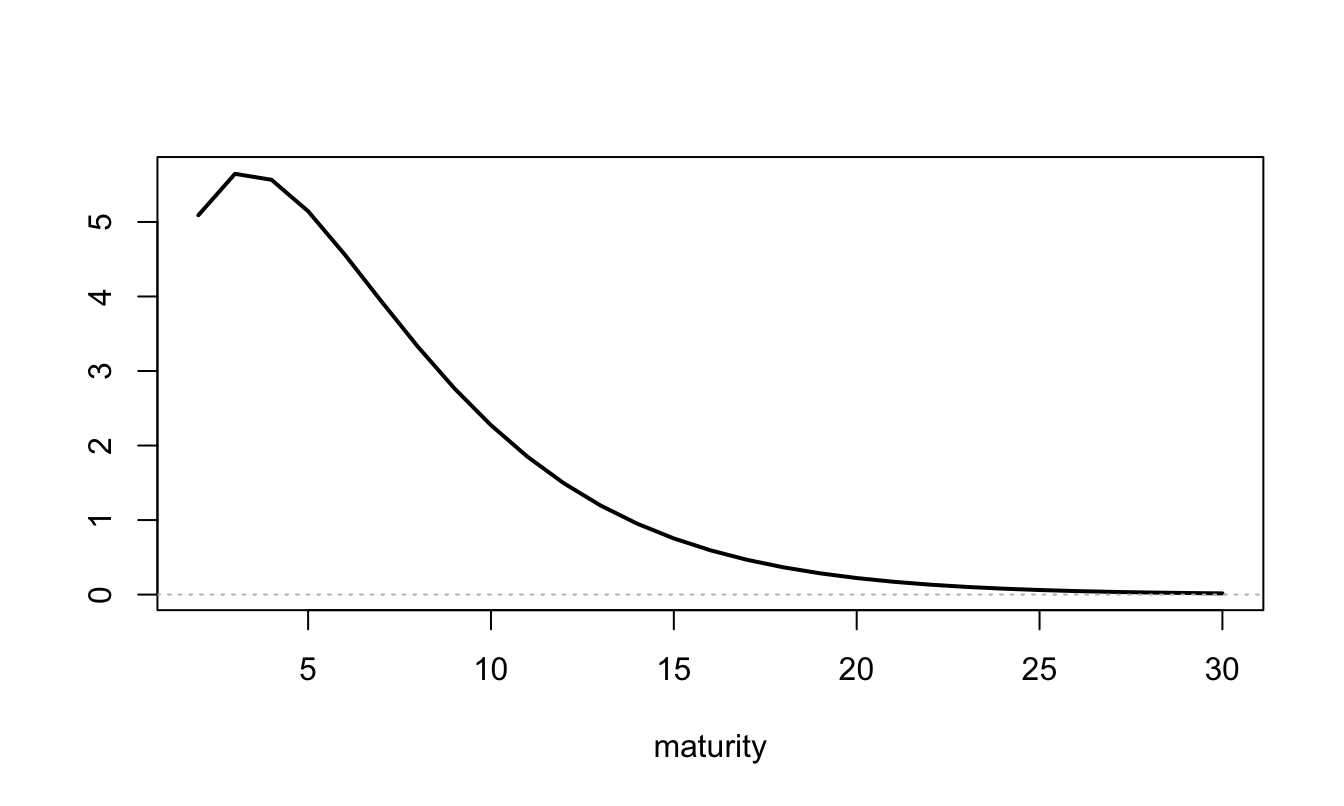
\includegraphics[width=0.95\linewidth]{TSM_files/figure-latex/VV1-1} \caption{Specification of the $\beta_{n,2}$, $n\ge 2$, that specify the influence of the supply factor ($f_{2,t}$) on bond supplies (the $s_{n,t}$'s).}\label{fig:VV1}
\end{figure}

Let us solve the model. Once it is done, let us determine the values of \(\alpha_1\) and \(\beta_1\) that guarantee that \(\sum_n z_{n,t}=1\) (see the discussion above):

\begin{Shaded}
\begin{Highlighting}[]
\NormalTok{RES }\OtherTok{\textless{}{-}} \FunctionTok{solve\_model}\NormalTok{(model,}\AttributeTok{indic.print =} \ConstantTok{FALSE}\NormalTok{)}
\NormalTok{alpha1 }\OtherTok{\textless{}{-}}\NormalTok{ RES}\SpecialCharTok{$}\NormalTok{lambdas}\SpecialCharTok{$}\NormalTok{alpha1}
\NormalTok{beta1  }\OtherTok{\textless{}{-}}\NormalTok{ RES}\SpecialCharTok{$}\NormalTok{lambdas}\SpecialCharTok{$}\NormalTok{beta1}
\NormalTok{Alpha[}\DecValTok{1}\NormalTok{] }\OtherTok{\textless{}{-}}\NormalTok{ alpha1}
\NormalTok{Beta[}\DecValTok{1}\NormalTok{,] }\OtherTok{\textless{}{-}}\NormalTok{ beta1}
\FunctionTok{plot}\NormalTok{(}\DecValTok{1}\SpecialCharTok{:}\NormalTok{N,Beta[}\DecValTok{1}\SpecialCharTok{:}\NormalTok{N,}\DecValTok{2}\NormalTok{],}\AttributeTok{type=}\StringTok{"l"}\NormalTok{,}\AttributeTok{lwd=}\DecValTok{2}\NormalTok{,}\AttributeTok{xlab=}\StringTok{"maturity"}\NormalTok{,}\AttributeTok{ylab=}\StringTok{""}\NormalTok{)}
\FunctionTok{abline}\NormalTok{(}\AttributeTok{h=}\DecValTok{0}\NormalTok{,}\AttributeTok{col=}\StringTok{"grey"}\NormalTok{,}\AttributeTok{lty=}\DecValTok{3}\NormalTok{)}
\end{Highlighting}
\end{Shaded}

\begin{figure}
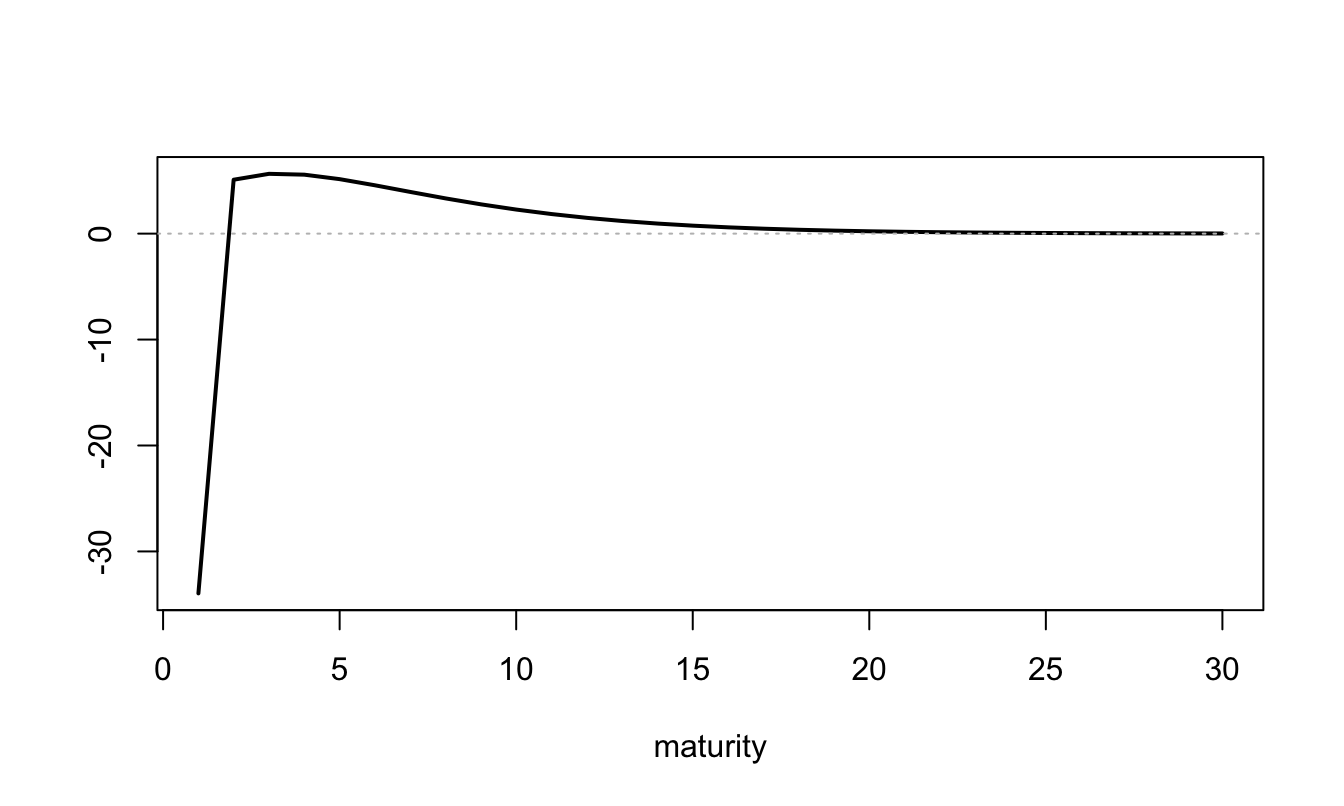
\includegraphics[width=0.95\linewidth]{TSM_files/figure-latex/VV2-1} \caption{Specification of the $\beta_{n,2}$, $n\ge 1$, that specify the influence of the supply factor ($f_{2,t}$) on bond supplies (the $s_{n,t}$'s).}\label{fig:VV2}
\end{figure}

Figure \ref{fig:VV3} shows the two term structures of factor loadings resulting from the model solution.

\begin{Shaded}
\begin{Highlighting}[]
\FunctionTok{par}\NormalTok{(}\AttributeTok{mfrow=}\FunctionTok{c}\NormalTok{(}\DecValTok{1}\NormalTok{,m))}
\ControlFlowTok{for}\NormalTok{(i }\ControlFlowTok{in} \DecValTok{1}\SpecialCharTok{:}\NormalTok{m)\{}
  \FunctionTok{plot}\NormalTok{(}\SpecialCharTok{{-}}\NormalTok{RES}\SpecialCharTok{$}\NormalTok{AB}\SpecialCharTok{$}\NormalTok{B[,i]}\SpecialCharTok{/}\DecValTok{1}\SpecialCharTok{:}\NormalTok{N,}\AttributeTok{type=}\StringTok{"l"}\NormalTok{,}\AttributeTok{lwd=}\DecValTok{2}\NormalTok{,}\AttributeTok{xlab=}\StringTok{"maturity"}\NormalTok{,}\AttributeTok{ylab=}\StringTok{""}\NormalTok{,}
       \AttributeTok{main =} \FunctionTok{paste}\NormalTok{(}\StringTok{"Factor "}\NormalTok{,i,}\AttributeTok{sep=}\StringTok{""}\NormalTok{))\}}
\end{Highlighting}
\end{Shaded}

\begin{figure}
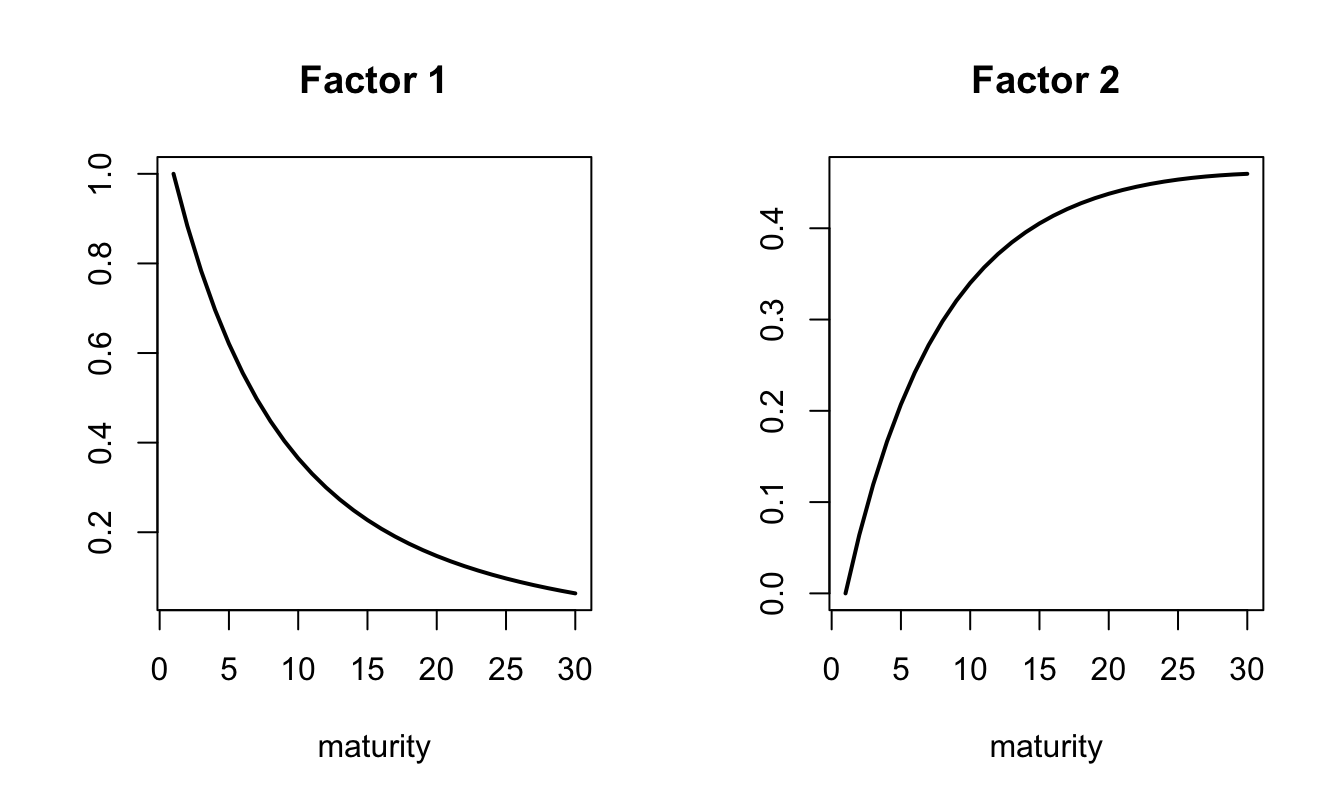
\includegraphics[width=0.95\linewidth]{TSM_files/figure-latex/VV3-1} \caption{Term structure of factor loadings.}\label{fig:VV3}
\end{figure}

Let us know determine the effect of an increase in the supply factor.

\begin{Shaded}
\begin{Highlighting}[]
\CommentTok{\# Shock:}
\NormalTok{shock }\OtherTok{\textless{}{-}} \FunctionTok{matrix}\NormalTok{(}\DecValTok{0}\NormalTok{,m,}\DecValTok{1}\NormalTok{)}
\NormalTok{shock[}\DecValTok{2}\NormalTok{] }\OtherTok{\textless{}{-}}\NormalTok{ .}\DecValTok{01}
\CommentTok{\# baseline yield curve:}
\NormalTok{avg.y      }\OtherTok{\textless{}{-}} \SpecialCharTok{{-}}\NormalTok{ RES}\SpecialCharTok{$}\NormalTok{AB}\SpecialCharTok{$}\NormalTok{A}\SpecialCharTok{/}\NormalTok{(}\DecValTok{1}\SpecialCharTok{:}\NormalTok{N)}
\CommentTok{\# yield curve after shock:}
\NormalTok{shock.y       }\OtherTok{\textless{}{-}} \SpecialCharTok{{-}} \DecValTok{1}\SpecialCharTok{/}\NormalTok{(}\DecValTok{1}\SpecialCharTok{:}\NormalTok{N) }\SpecialCharTok{*}\NormalTok{ (RES}\SpecialCharTok{$}\NormalTok{AB}\SpecialCharTok{$}\NormalTok{A }\SpecialCharTok{+}\NormalTok{ RES}\SpecialCharTok{$}\NormalTok{AB}\SpecialCharTok{$}\NormalTok{B }\SpecialCharTok{\%*\%}\NormalTok{ shock)}
\CommentTok{\# Quantitiies:}
\NormalTok{avg.z   }\OtherTok{\textless{}{-}}\NormalTok{ Alpha }\SpecialCharTok{{-}}\NormalTok{ Zeta }\SpecialCharTok{*}\NormalTok{ avg.y}
\NormalTok{shock.z }\OtherTok{\textless{}{-}}\NormalTok{ Alpha }\SpecialCharTok{+}\NormalTok{ Beta }\SpecialCharTok{\%*\%}\NormalTok{ shock }\SpecialCharTok{{-}}\NormalTok{ Zeta }\SpecialCharTok{*}\NormalTok{ shock.y}

\FunctionTok{par}\NormalTok{(}\AttributeTok{mfrow=}\FunctionTok{c}\NormalTok{(}\DecValTok{1}\NormalTok{,}\DecValTok{2}\NormalTok{))}
\FunctionTok{plot}\NormalTok{(avg.y,}\AttributeTok{type=}\StringTok{"l"}\NormalTok{,}\AttributeTok{ylim=}\FunctionTok{c}\NormalTok{(.}\DecValTok{95}\SpecialCharTok{*}\FunctionTok{min}\NormalTok{(avg.y,shock.y),}\FloatTok{1.05}\SpecialCharTok{*}\FunctionTok{max}\NormalTok{(avg.y,shock.y)),}
     \AttributeTok{lwd=}\DecValTok{2}\NormalTok{,}\AttributeTok{xlab=}\StringTok{"maturity"}\NormalTok{,}\AttributeTok{ylab=}\StringTok{"yields"}\NormalTok{,}\AttributeTok{las=}\DecValTok{1}\NormalTok{)}
\FunctionTok{lines}\NormalTok{(shock.y,}\AttributeTok{lty=}\DecValTok{2}\NormalTok{,}\AttributeTok{lwd=}\DecValTok{2}\NormalTok{,}\AttributeTok{col=}\StringTok{"red"}\NormalTok{)}

\FunctionTok{plot}\NormalTok{(avg.z,}\AttributeTok{ylim=}\FunctionTok{c}\NormalTok{(}\FunctionTok{min}\NormalTok{(avg.z,shock.z),}\FloatTok{1.1}\SpecialCharTok{*}\FunctionTok{max}\NormalTok{(avg.z,shock.z)),}\AttributeTok{pch=}\DecValTok{19}\NormalTok{,}
     \AttributeTok{xlab=}\StringTok{"maturity"}\NormalTok{,}\AttributeTok{ylab=}\StringTok{"Fraction of portfolio"}\NormalTok{,}\AttributeTok{las=}\DecValTok{1}\NormalTok{)}
\FunctionTok{points}\NormalTok{(shock.z,}\AttributeTok{lty=}\DecValTok{2}\NormalTok{,}\AttributeTok{col=}\StringTok{"red"}\NormalTok{,}\AttributeTok{lwd=}\DecValTok{2}\NormalTok{)}
\FunctionTok{abline}\NormalTok{(}\AttributeTok{h=}\DecValTok{0}\NormalTok{,}\AttributeTok{col=}\StringTok{"grey"}\NormalTok{,}\AttributeTok{lty=}\DecValTok{3}\NormalTok{)}
\end{Highlighting}
\end{Shaded}

\begin{figure}
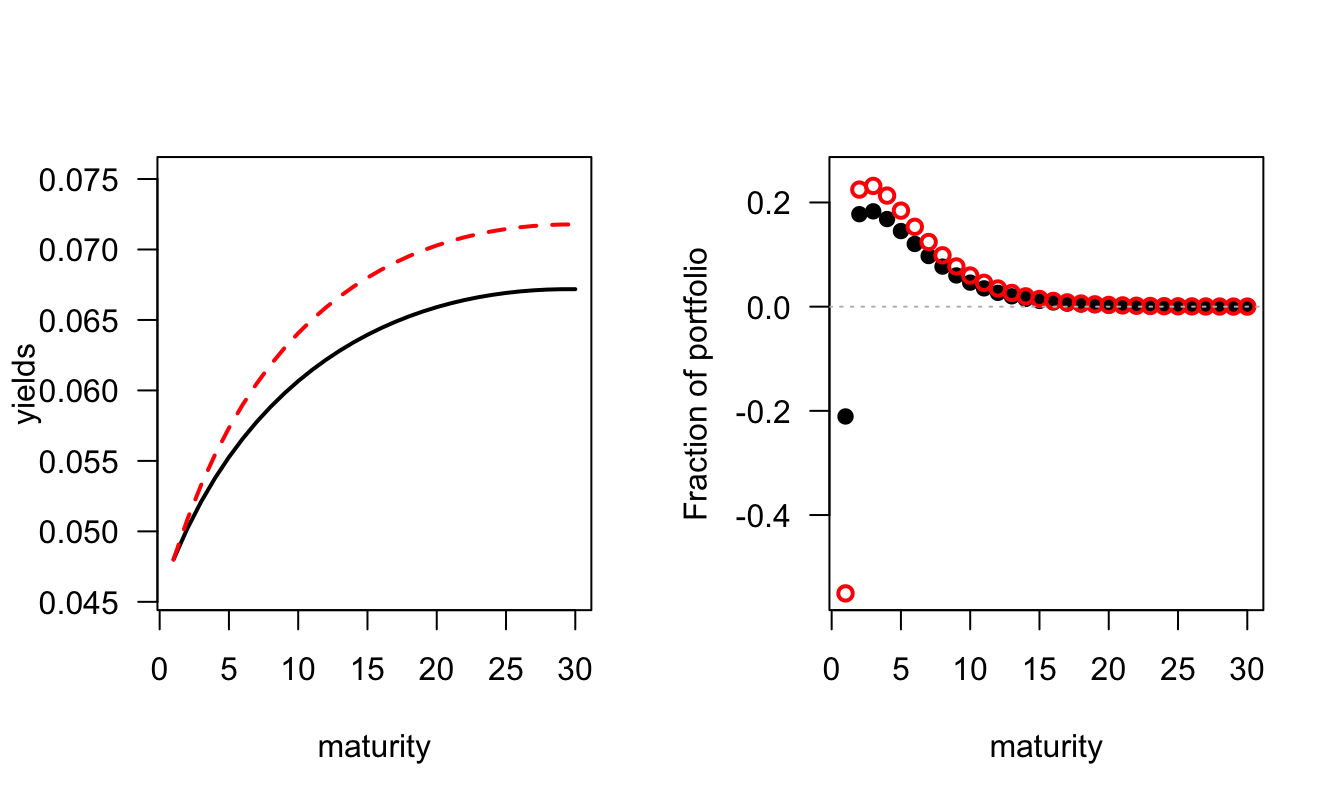
\includegraphics[width=0.95\linewidth]{TSM_files/figure-latex/VV4-1} \caption{Effect of a shock on the second factor. The left hand side plot shows the yield curve effect; the right hand side plot shows the effect on the composition of arbitrageurs' bond portfolio. For the two plots, the black lines indicate the unconditional average and the red line shows the curves conditional on the shock.}\label{fig:VV4}
\end{figure}

\hypertarget{appendix}{%
\section{Appendix}\label{appendix}}

\hypertarget{SDFEZ}{%
\subsection{SDF in the CES Epstein-Zin Context}\label{SDFEZ}}

We denote by \(\pi_t(x_{t+1})\) the price of an asset that provides the payoff \(x_{t+1}\) at date \(t+1\) (as of date \(t\), this payoff may be random). If one purchases \(\varepsilon\) units of this asset and consumes them at date \(t+1\), the intertemporal utility becomes \(F(C_t\color{blue}{ - \varepsilon \pi_t(x_{t+1})},R_t(F(C_{t+1}+\color{blue}{\varepsilon x_{t+1}},R_{t+1}(U_{t+2}))))\).

If \(\pi_t(x_{t+1})\) is the equilibrium price of the asset, then agents should be indifferent between buying a small amount of this asset and not. That is, we should have:
\[
F(C_t,R_t(F(C_{t+1},R_{t+1}(U_{t+2})))) =
F(C_t {\color{blue} - \varepsilon \pi_t(x_{t+1})},R_t(F(C_{t+1}+{\color{blue}\varepsilon x_{t+1}},R_{t+1}(U_{t+2})))).
\]
Let's compute the first-order Taylor expansion of right-hand side term w.r.t. \(\varepsilon\). To begin with, we have:
\[
F(C_{t+1}+{\color{blue}\varepsilon x_{t+1}},R_{t+1}(U_{t+2})) = U_{t+1} + \varepsilon x_{t+1} (1-\beta) C_{t+1}^{-\rho}U_{t+1}^\rho + o(\varepsilon).
\]
Now,
\[
F(C_{t+1}+{\color{blue}\varepsilon x_{t+1}},R_{t+1}(U_{t+2}))^{1-\gamma} = U_{t+1}^{1-\gamma} + \varepsilon x_{t+1}  (1-\beta) C_{t+1}^{-\rho}U_{t+1}^{\rho-\gamma} + o(\varepsilon).
\]
Then,
\[
\mathbb{E}_t \left( F(C_{t+1}+{\color{blue}\varepsilon x_{t+1}},R_{t+1}(U_{t+2}))^{1-\gamma} \right)^{\frac{1}{1-\gamma}}=R_t(U_{t+1}) + \varepsilon R_t(U_{t+1})^{\gamma} \mathbb{E}_t \left(  x_{t+1} (1-\beta) C_{t+1}^{-\rho} U_{t+1}^{\rho-\gamma} \right).
\]
Therefore, \(F(C_t{\color{blue} - \varepsilon \pi_t(x_{t+1})},R_t(F(C_{t+1}+{\color{blue}\varepsilon x_{t+1}},R_{t+1}(U_{t+2}))))\) is equal to \(F(C_t,R_t(U_{t+1}))+\)
\[
\varepsilon R_t(U_{t+1})^{\gamma - \rho} \mathbb{E}_t \left(  x_{t+1} (1-\beta) C_{t+1}^{-\rho} U_{t+1}^{\rho-\gamma} \right) U_t^{\rho}
- \varepsilon \pi_t(x_{t+1}) (1-\beta) C_t^{-\rho} U_t^{\rho} + o(\varepsilon),
\]
which gives \eqref{eq:SSS}.

\hypertarget{TSModels}{%
\chapter{No-arbitrage models of the term struture of risk-free yields}\label{TSModels}}

\hypertarget{RFIntroduction}{%
\section{Introduction}\label{RFIntroduction}}

Risk-free yields are the yields-to-maturity associated with bonds that carry no default and/or liquidity risks. Bonds issued by sovereign entities with top credit quality are usually considered to be risk-free. Because of call-margins mechanisms, swap rates are also used as risk-free benchmarks \citep{Duffie_Stein_2015} (see Subsection \ref{Swaps}). (Credit and liquidity risks are covered in Section \ref{CreditLiRisks}.)

An important share of the term-structure literature pertains to the modelling of risk-free yields. Some models explicitly involve macroeconomic factors; this can be done in a reduced-form way (e.g., \citet{Ang_Piazzesi_2003}) or in a more structural way, in the context of the equilibrium term-structure approaches (e.g., \citet{Bansal_Shaliastovich_2013}, see Example \ref{exm:BS2013}) or even in the context of dynamic stochastic general equilibrium models (e.g., \citet{Hordahl_Tristani_veston_2008}, \citet{DewBecker_2014}). Many studies feature purely latent factors, with no explicit macroeconomic interpretation (e.g., \citet{Duffie_Singleton_1997}, \citet{Joslin_Singleton_Zhu_2011}). The latter are sometimes called \emph{yield-only} models.

In this section, we consider term structure of zero-coupon yields, which are basic objects from which one can price any stream of fixed payoffs that will be settled at fixed future dates. These yields are usually not directly observed in the market. As a result, they have to be constructed in the first place; Appendix \ref{constructing} briefly presents approaches used for that purpose.

Under regularity and no-arbitrage assumptions, the price of a risk-free zero coupon bond, and the associated yield-to-maturity, satisfy (see Eq. \eqref{eq:ihandM}):
\begin{eqnarray}
B_{t,h} &=& \mathbb{E}_t (\mathcal{M}_{t,t+h})\nonumber\\
&=& \mathbb{E}^{\mathbb{Q}}_t \exp(-i_t -i_{t+1}-\dots-i_{t+h-1})\nonumber\\
i_{t,h} &=& - \frac{1}{h} \log B_{t,h}, \label{eq:stdbondRFchapter}
\end{eqnarray}
where \(\mathcal{M}_{t,t+h}\) is the (strictly positive) stochastic discount factor between dates \(t\) and \(t+h\), and where the risk neutral measure \(\mathbb{Q}\) is defined with respect to the physical measure \(\mathbb{P}\) by means of the Radon-Nikodym derivative \(\mathcal{M}_{t,t+1}\big/\mathbb{E}_t(\mathcal{M}_{t,t+1})\).\footnote{That is, for any random variable \(X_{t+1}\):
  \[
  \mathbb{E}^{\mathbb{Q}}_t(X_{t+1})=\mathbb{E}_t\left(X_{t+1}\frac{\mathcal{M}_{t,t+1}}{\mathbb{E}_t(\mathcal{M}_{t,t+1})}\right).
  \]}

Term structure models are often used to extract \emph{term premiums} from observed yields-to-maturity. Term premiums are those components of yields that would not exist if investors were not risk-averse (see, e.g., Subsection \ref{TSCCAPM}).

If agents were not risk averse, i.e., under the \emph{Expectation Hypothesis (EH)}, we would have \(\mathcal{M}_{t,t+1} = \exp(- i_t)\) and \(\mathbb{P} \equiv \mathbb{Q}\); \(B_{t,h}\) would then be equal to:
\begin{equation}
B^{EH}_{t,h} := \mathbb{E}_t \exp(-i_{t}-i_{t+1}-\dots-i_{t+h-1}).\label{eq:stdbondRFchapterP}
\end{equation}
The (counterfactual) maturity-\(h\) yield-to-maturity would then be:
\begin{eqnarray}
i^{EH}_{t,h} &=& -\frac{1}{h}\log \left( \mathbb{E}_t \exp(-i_t-\dots-i_{t+h-1})\right)\nonumber\\
&\approx& \frac{1}{h}\mathbb{E}_t(i_t + \dots + i_{t+h-1}).\label{eq:REH}
\end{eqnarray}

Using the previous notations, the term premium is usually defined as:
\begin{eqnarray}
TP_{t,h} &=& \underbrace{- \frac{1}{h} \log  \mathbb{E}^{\mathbb{Q}}_t \exp(-i_{t+1}-\dots-i_{t+h-1})}_{=i_{t,h}} - \nonumber \\
&& \underbrace{- \frac{1}{h}  \log  \mathbb{E}_t \exp(-i_{t+1}-\dots-i_{t+h-1}).}_{=i^{EH}_{t,h}}\label{eq:TP}
\end{eqnarray}

A term premium is a specific type of risk premium (see Def. \ref{def:RPremium}), in the sense that it reflects changes between the price of an asset (a bond here, \(B_{t,h}\)) and the counterfactual we would observe if agents were not risk averse (\(B_{t,h}^{EH}\), here).

Economically, what accounts for term premiums? To address this in a comprehensive way, one needs to resort to structural approaches (see Section \ref{Structural}). A short reply is that a long-term bond is never ``risk-free'' as it is exposed to the interest-rate risk; and that investors are averse to this risk, hence the term premiums. Take a two-period bond; using \eqref{eq:basicAAA}, we have:
\begin{equation}
B_{t,2} = \underbrace{\mathbb{E}_t(\exp(-i_t-i_{t+1}))}_{= B^{EH}_{t,2}} + \mathbb{C}ov_t(\mathcal{M}_{t,t+1},\underbrace{\exp(-i_{t+1})}_{=B_{t+1,1}}).\label{eq:Bt2}
\end{equation}
Therefore \(B_{t,2} \ne B_{t,2}^{EH}\) as soon as \(\mathcal{M}_{t,t+1}\) and \(i_{t+1}\) are conditionally correlated, which is likely to be the case (see, e.g., the CCAPM case in Subsection \ref{TSCCAPM}).

In the following subsections, we describe statistical approaches that have been used to estimate term premiums. These approaches are usually silent about the drivers of the term premiums. Eq \eqref{eq:Bt2} provides some insights regarding the sources of fluctuations of term premiums: interest rate volatility, SDF volatility (that may depend on risk aversion, see, e.g., the Epstein-Zin case in \eqref{eq:sdfAbc}), the correlation between interest rates and the SDF.

Under EH, investors are willing to buy a maturity-\(h\) bond as long as its expected return is---up to Jensen's inequality---equal to the average of future short-term rates. (Hence the definition of \(i^{EH}_{t,h}\), see Eq. \eqref{eq:REH}.) The fact that \(TP_{t,h}>0\) (say) means that investors are willing to buy the maturity-\(h\) bond only if its return is, on average, higher than expected future short-term rates; it corresponds to a situation where investors consider that long-term bonds tend to lose value in \emph{bad states of the world} (i.e., states of high marginal utility) and want to be compensated for that.

\begin{definition}[Risk premium, in the general case]
\protect\hypertarget{def:RPremium}{}\label{def:RPremium}According to \eqref{eq:basic}, under the absence of arbitrage opportunities, the price of any asset \(j\) satisfies:
\begin{equation}
p_{jt} = \mathbb{E}_t(\mathcal{M}_{t,t+1} p_{j,t+1}),\label{eq:basicAAA}
\end{equation}
or, equivalently,
\[
p_{jt} = \exp(-i_t)\mathbb{E}^{\mathbb{Q}}_t(p_{j,t+1}),
\]
where the risk neutral measure \(\mathbb{Q}\) is defined with respect to the physical measure \(\mathbb{P}\) by means of the Radon-Nikodym derivative \(\mathcal{M}_{t,t+1}\big/\mathbb{E}_t(\mathcal{M}_{t,t+1})\).\footnote{That is, for any random variable \(X_{t+1}\):
  \[
  \mathbb{E}^{\mathbb{Q}}_t(X_{t+1})=\mathbb{E}_t\left(X_{t+1}\frac{\mathcal{M}_{t,t+1}}{\mathbb{E}_t(\mathcal{M}_{t,t+1})}\right).
  \]}

Eq. \eqref{eq:basicAAA} rewrites:
\[
p_{jt} =  \mathbb{C}ov_t(\mathcal{M}_{t,t+1}, p_{j,t+1}) + \mathbb{E}_t(\mathcal{M}_{t,t+1})\mathbb{E}_t( p_{j,t+1})
\]
or
\begin{equation}
p_{jt} = \underbrace{\exp(-i_t)\mathbb{E}_t( p_{j,t+1})}_{=p^{EH}_{jt}} + \underbrace{\mathbb{C}ov_t(\mathcal{M}_{t,t+1}, p_{j,t+1})}_{\mbox{Risk premium}}.\label{eq:CovRP}
\end{equation}
If investors were not risk-averse, then we would have \(p_{jt} = p^{EH}_{jt}\). The SDF is high (resp. low) in bad (resp. good) states of the world (states of high marginal utility in the equilibrium approach). Hence, we have \(p_{jt}< p^{EH}_{jt}\) if asset \(j\) tends to pay less in bad states of the world (i.e., if \(\mathbb{C}ov_t(\mathcal{M}_{t,t+1}, p_{j,t+1})<0\)).
\end{definition}

\begin{example}[Testing the Expectation Hypothesis]
\protect\hypertarget{exm:TestingEH}{}\label{exm:TestingEH}Several studies have employed regression analysis to test the Expectation Hypothesis, e.g., \citet{Campbell_Shiller_1991} and \citet{Cochrane_Piazzesi_2005}. Let us focus on the former study. \citet{Campbell_Shiller_1991} note that, if agents were risk-neutral, we would have:
\[
B_{t,n} = \exp(-i_{t,m})\mathbb{E}_t(B_{t+m,n-m}).
\]
This would imply:
\[
-n i_{t,n} = -i_{t,m} + \log \mathbb{E}_t[\exp(-(n-m) i_{t+m,n-m})].
\]
Up to the Jensen inequality, and taking expectations on both sides, we get:
\[
-n i_{t,n} \approx \mathbb{E}_t(-i_{t,m} -(n-m) i_{t+m,n-m}).
\]
After having reorganized:
\begin{equation}
\mathbb{E}_t(i_{t+m,n-m}-i_{t,n}) \approx \frac{i_{t,n}-i_{t,m}}{n-m}.\label{eq:CStheo}
\end{equation}

\citet{Campbell_Shiller_1991} have used the previous expression to test for the Expectation hypothesis. Formally, they run the following regressions for different values of \(n\) and \(m\):
\[
i_{t+m,n-m}-i_{t,n} = \phi_n\frac{i_{t,n}-i_{t,m}}{n-m} + \varepsilon_{t+m}.
\]

According to \eqref{eq:CStheo}, under the Expectation Hypothesis, we should have \(\phi_{n,m} \approx 1\). But they do find that the \(\phi_{n,m}\) are statistically lower than one. Besides, they find that, for a given holding period \(m\), the term structure of the \(\phi_{n,m}\) decreases with the maturity \(n\). Figure \ref{fig:CSregressions} shows the results of such regressions on a more recent period. It appears that the original results of \citet{Campbell_Shiller_1991} are still valid.

\textbackslash begin\{figure\}
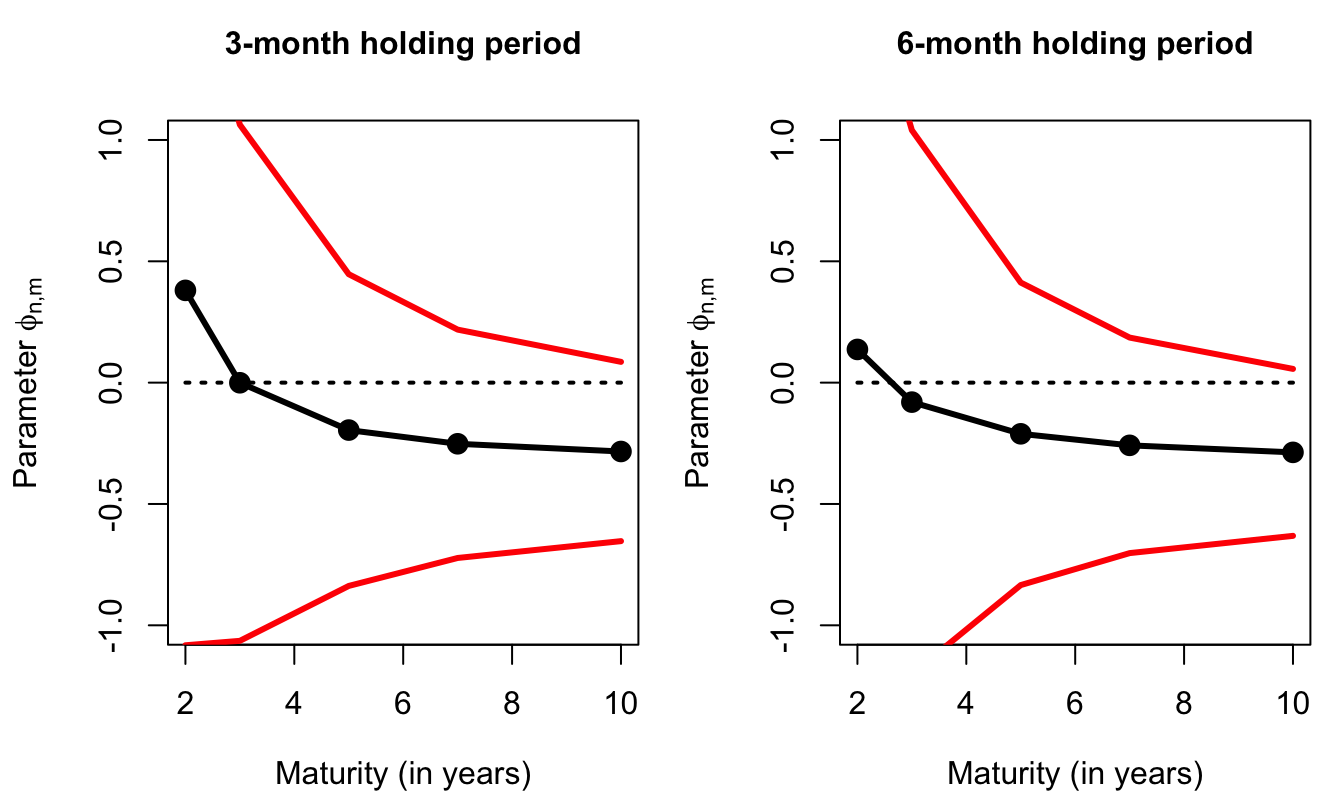
\includegraphics[width=0.95\linewidth]{TSM_files/figure-latex/CSregressions-1} \textbackslash caption\{Regressions as in Campbell and Shiller (1991). Data are at the monthly frequency; they are collected from the FRED database. The estimation period starts in 1990. The figure reports 90\% confidence intervals of the \(\phi_{n,m}\) parameter estimates (Newey-West robust standard deviations).\}\label{fig:CSregressions}
\textbackslash end\{figure\}
\end{example}

Before turning to the no-arbitrage term structure models, note that \eqref{eq:TP} implies that term premium estimates are directly available if we have good approximations for the expected future short term rates (i.e., \(i_{t,h}^{EH}\)). Some surveys offer such proxies. It is for instance the case of the \href{https://www.philadelphiafed.org/surveys-and-data/bill10}{Philadelphia Fed SPF}, that provides expectations of the short-term rate over the next 10 years (see Figure \ref{fig:modeFreeTP}). However, there is only one release per year for this survey.

\begin{figure}
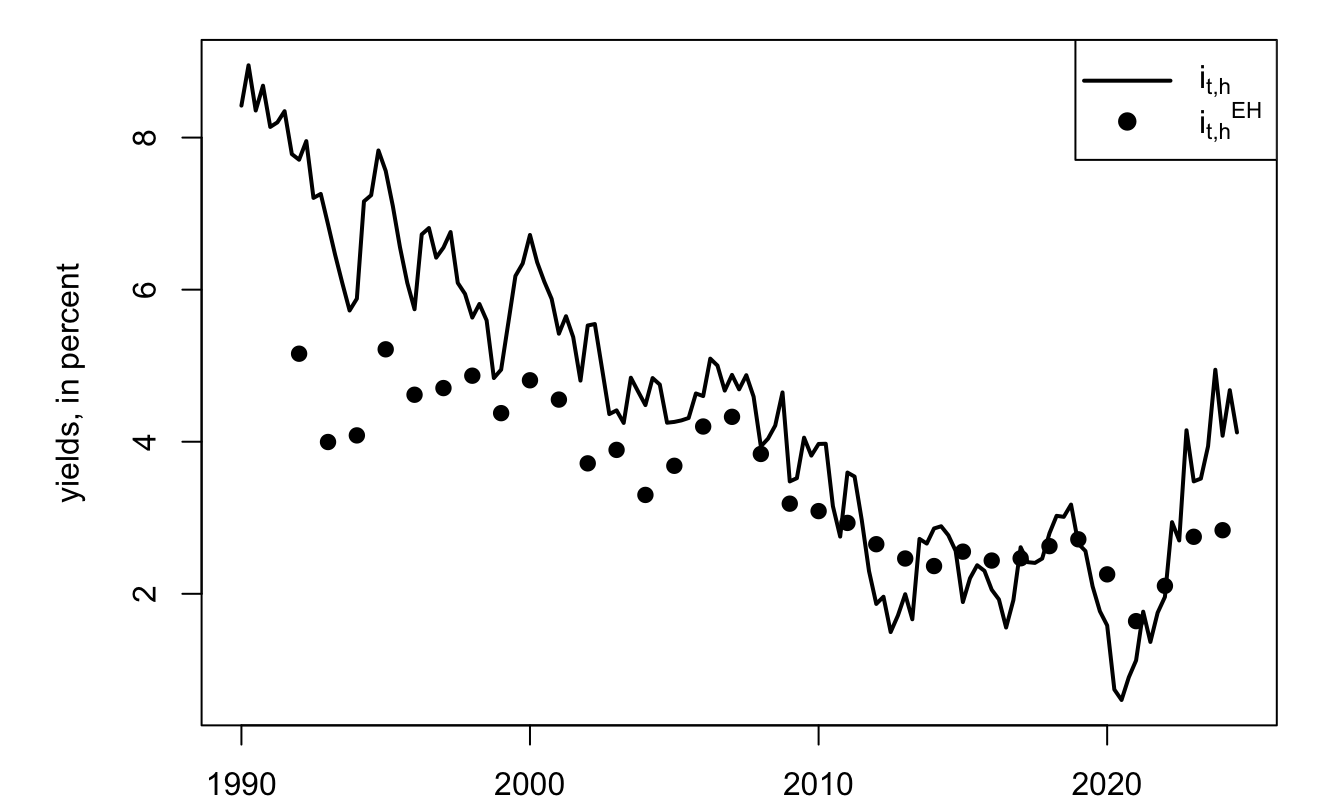
\includegraphics[width=0.95\linewidth]{TSM_files/figure-latex/modeFreeTP-1} \caption{Sources: SPF Philadelphia for $i_{t,h}^{EH}$ (ticker BILL10) and FRED database for $i_{t,h}$ (ticker THREEFY10).}\label{fig:modeFreeTP}
\end{figure}

In the same spirit, Figure \ref{fig:modeFreeIRP} compares the 10-year breakeven rate of inflation (\(i_{t,h}- r_{t,h}\)), also called inflation compensation, with the expected annualized inflation over the next 10 years. The difference between the line and the dots is the \emph{inflation risk premium}, defined as:
\[
IRP_{t,h} = i_{t,h} - r_{t,h} - \mathbb{E}_t(\pi_{t,t+h}),
\]
where \(\pi_{t,t+h}\) denotes the annualized inflation rate between dates \(t\) and \(t+h\).

Figure \ref{fig:modeFreeIRP} shows that the inflation risk premium has often been negative in recent years, suggesting a perceived importance of demand shocks in the economy.

\begin{figure}
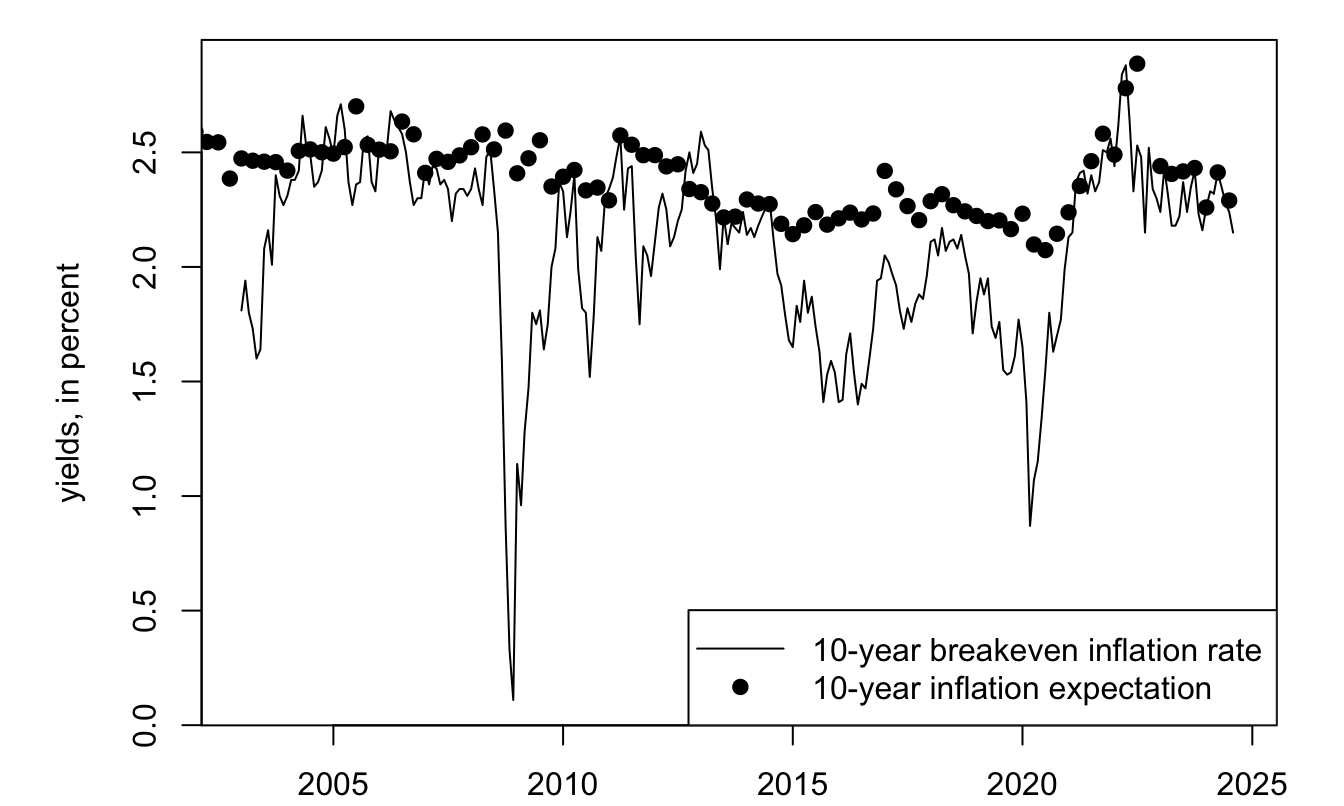
\includegraphics[width=0.95\linewidth]{TSM_files/figure-latex/modeFreeIRP-1} \caption{Sources: SPF Philadelphia for the 10-year inflation expectation (ticker CPI19) and FRED database for $i_{t,h}$ (ticker DGS10) and for $r_{t,h}$ (ticker DFII10).}\label{fig:modeFreeIRP}
\end{figure}

\hypertarget{RiskFreeAffine}{%
\section{The Affine Case}\label{RiskFreeAffine}}

\hypertarget{AffineYields}{%
\subsection{Affine yields}\label{AffineYields}}

In this subsection, we consider the case where the state vector \(w_t\) is affine under both \(\mathbb{P}\) and \(\mathbb{Q}\). If the nominal short-term rate is affine in \(w_t\), i.e., if \(i_t = \omega_0 + \omega'_1 w_t\), then (see \eqref{eq:ihandM}):
\begin{eqnarray*}
B_{t,h} &=& \mathbb{E}^{\mathbb{Q}}_t \exp (-i_{t}-\dots-i_{t+h-1})\\
&=& \exp(-h\omega_0 - \omega'_1 w_t) \color{blue}{\mathbb{E}^{\mathbb{Q}}_t \exp (- \omega'_1 w_{t+1}-\dots- \omega'_1 w_{t+h-1})}.
\end{eqnarray*}
The (blue) expectation is easily computed using the recursive equations of Proposition \ref{prp:reverseMLT} (see Example \ref{exm:nominalBth}), leading to:
\begin{equation}
i_{t,h}= -  \frac{1}{h}   \log   B_{t,h} = a_h'w_t + b_h.\label{eq:RthAB}
\end{equation}
It is easily seen that we can also get:
\begin{equation}
i^{EH}_{t,h} = {a^{EH}_h}'w_t + b^{EH}_h.\label{eq:RthABEH}
\end{equation}
Moreover, if inflation is also affine in \(w_t\), i.e., if \(\pi_{t} = \bar\omega_0 + \bar\omega'_1 w_t\), then real yields are given by:
\begin{eqnarray*}
\mathcal{B}_{t,h} &=& \mathbb{E}^{\mathbb{Q}}_t \exp(-i_{t}-\dots-i_{t+h-1}+\pi_{t+1}+\dots+\pi_{t+h})
\end{eqnarray*}
(see Example \ref{exm:realBth}) which also leads to:
\begin{equation}
r_{t,h} = -  \frac{1}{h}   \log   \mathcal{B}_{t,h} = \bar{a}_h'w_t + \bar{b}_h.\label{eq:RbarthAB}
\end{equation}
Eqs. \eqref{eq:RthAB} and \eqref{eq:RthABEH} imply that term premiums are affine in \(w_t\) (see Eq. \eqref{eq:TP}). Specifically:
\[
TP_{t,h} = i_{t,h} - i^{EH}_{t,h} = b_h - b_h^{EH} + (a_h - a_h^{EH})'w_t.
\]

\begin{quote}
The same approach can be employed to compute real term premiums (\(r_{t,h} - r^{EH}_{t,h}\)), and inflation term premiums(\((i_{t,h}-r_{t,h}) - (i^{EH}_{t,h}-r^{EH}_{t,h})\)).
\end{quote}

Expected excess returns resulting from holding zero-coupon bonds are also affine in \(w_t\). Indeed, holding a maturity-\(h\) zero-coupon bond for one period provides the following expected gross return:
\[
\mathbb{E}_t\left(\frac{B_{t+1,h-1}}{B_{t,h}}\right) = \mathbb{E}_t\left(\exp(b_{h-1} - b_h + a_{h-1}'w_{t+1} - a_h'w_{t})\right),
\]
which is clearly exponential affine in \(w_t\) if \(w_t\) is an affine process. Therefore, the log expected excess return, that is:
\[
\log \mathbb{E}_t\left(\frac{B_{t+1,h-1}}{B_{t,h}}\right) - i_t
\]
is also affine in \(w_t\). This is exploited in the estimation approach proposed by \citet{Adrian_Crump_Moench_2013}.

Moreover, \emph{conditional expectations} of future interest rates (real or nominal) and of term premiums are also affine in \(w_t\). In particular:
\begin{equation}
\mathbb{E}_t[i_{t+k,h}] = \mathbb{E}_t[{a_h}'w_{t+k} + b_h] = {a_h}'\mathbb{E}_t(w_{t+k}) + b_h,\label{eq:condmeanRth}
\end{equation}
and \(\mathbb{E}_t(w_{t+k})\) is affine in \(w_t\) (see Eq. \eqref{eq:condmean}). This can notably be used at the estimation stage, if one wants to fit survey data (see Subsection \ref{EstimationPersistency}).

Similarly, \emph{conditional variances} of future interest rates (real or nominal) and of term premiums are affine in \(w_t\). In particular:
\begin{equation}
\mathbb{V}ar_t[i_{t+k,h}] = \mathbb{V}ar_t[{a_h}'w_{t+k} + b_h] = {a_h}'\mathbb{V}ar_t(w_{t+k})a_h,\label{eq:condvarRth}
\end{equation}
where the components of \(\mathbb{V}ar_t(w_{t+k})\) (and therefore \(\mathbb{V}ar_t[i_{t+k,h}]\)) is affine in \(w_t\) (see Eq. \eqref{eq:condvar}). This can also be used at the estimation stage, if one wants to fit (proxies of) conditional variances \citep{zarg_2017}.

\hypertarget{maximum-sharpe-ratio}{%
\subsection{Maximum Sharpe ratio}\label{maximum-sharpe-ratio}}

In an affine model, the maximum Sharpe ratio is easily computed. This has been noted early by \citet{Duffee_2010} for the Gaussian model; \citet{Gourieroux_Monfort_Mouabbi_Renne_2021} and \citet{Pallara_Renne_2023} use it in more sophisticated affine models.

Let us derive the maximum Sharpe ratio in the context of a genral affine framework. Eq. \eqref{eq:CovRP} implies that
\[
\mathbb{E}_t\underbrace{\left(\frac{p_{j,t+1}}{p_{j,t}} - \exp(i_t)\right)}_{=xs_{j,t+1},\mbox{ excess return}} =  - \exp(i_t) \mathbb{C}ov_t\left(\mathcal{M}_{t,t+1},\frac{p_{j,t+1}}{p_{j,t}}\right),
\]
and, using \(|\mathbb{C}ov(X,Y)| \le \sqrt{\mathbb{V}ar(X)\mathbb{V}ar(Y)}\), we get the \citet{Hansen_Jagannathan_1991} bound:
\begin{equation}
\underbrace{\frac{\mathbb{E}_t(xs_{j,t+1})}{\sqrt{\mathbb{V}ar_t(xs_{j,t+1})}}}_{\mbox{Sharpe ratio}} \le \underbrace{\frac{\sqrt{\mathbb{V}ar_t(\mathcal{M}_{t,t+1})}}{\mathbb{E}_t(\mathcal{M}_{t,t+1})}}_{\mbox{Maximum Sharpe ratio}}.
\end{equation}

If the SDF is given by \(\mathcal{M}_{t,t+1} = \exp[-i_{t}+\alpha'_tw_{t+1}-\psi_t(\alpha_t)]\) (Eq. \eqref{eq:keySDF}), and using that \(\mathbb{E}_t(\mathcal{M}_{t,t+1}^2)=\exp(-2i_t+\psi_t(2\alpha_t)-2\psi_t(\alpha_t))\) we get:
\[
\mbox{Maximum Sharpe ratio} = \sqrt{\exp(\psi_t(2\alpha_t)-2\psi_t(\alpha_t)) - 1}.
\]

\hypertarget{RiskFreeGaussian}{%
\section{Gaussian Affine Term Structure Model}\label{RiskFreeGaussian}}

The Gaussian Affine Term Structure Model (GATSM) is a \emph{workhorse} model, widely used in academic and economic-policy circles. In a GATSM, \(w_t\) follows a Gaussian vector autoregressive model, and is therefore affine under \(\mathbb{P}\). The SDF is exponential affine in \(w_t\), which implies that process \(w_t\) is also affine under \(\mathbb{Q}\) (shown below). Since the components of \(w_t\) are valued in \(\mathbb{R}\), one can easily introduce macro-factors among the state variables.

Let us be more specific. The state vector \(w_t\) follows:
\begin{equation}
w_{t+1} = \mu + \Phi w_{t} + \Sigma^{1/2} \varepsilon_{t+1}, \mbox{ where } \varepsilon_{t} \sim  i.i.d. \mathcal{N}(0,Id).\label{eq:GaussianVAR1}
\end{equation}
(The fact that we consider a VAR(1) process is without loss of generality since a VAR(p) admits a VAR(1) companion representation.)

This implies the following log-Laplace transform for \(w_t\) (see Example \ref{exm:GVAR1}):
\[
\psi_t(u) = \log \mathbb{E}_t(\exp(u'w_{t+1})|\underline{w_t}) = \color{blue}{u'\mu + u'\Phi w_t + \frac{1}{2}u'\Sigma'u}.
\]
Using the notations of \eqref{eq:keySDF}, the SDF is defined as:
\[
\mathcal{M}_{t,t+1} = \exp(- i_t + \alpha_t'w_{t+1} - \psi_t(\alpha_t)), \mbox{ where } \alpha_t = \alpha_0 + \alpha_1'w_t.
\]

In that case, using \eqref{eq:transfoPQ}, we get:
\begin{eqnarray*}
\psi_t^{\mathbb{Q}}(u) &=& \psi_t(u + \alpha_t) - \psi_t(\alpha_t)\\
&=& (u + \alpha_t)'\mu + (u + \alpha_t)'\Phi w_t + \frac{1}{2}(u + \alpha_t)'\Sigma(u + \alpha_t) \\
&& - \left(\alpha_t'\mu + \alpha_t'\Phi w_t + \frac{1}{2}\alpha_t'\Sigma\alpha_t\right) \\
&=& \color{blue}{u' \left(\mu + \Sigma \alpha_0 \right) + u'(\Phi + \Sigma \alpha_1')w_t  + \frac{1}{2}u'\Sigma'u}.
\end{eqnarray*}
This is the Laplace tranform of a Gaussian VAR process (see Example \ref{exm:GVAR1}); accordingly, the \(\mathbb{Q}\)-dynamics of \(w_t\) is:
\[
w_{t+1} = \mu + \Sigma  \alpha_0 + (\Phi + \Sigma \alpha_1')  w_{t} + \Sigma^{1/2} \varepsilon^*_{t+1}, \mbox{ where } \varepsilon^*_{t} \sim  i.i.d. \mathcal{N}^{\mathbb{Q}}(0,Id).
\]
or
\begin{equation}
w_{t+1} = \mu^{\mathbb{Q}} + \Phi^{\mathbb{Q}} w_{t} + \Sigma^{1/2} \varepsilon^*_{t+1},\label{eq:GaussianQdyn}
\end{equation}
where
\[
\boxed{\mu^{\mathbb{Q}} = \mu + \Sigma  \alpha_0,\quad \mbox{and} \quad\Phi^{\mathbb{Q}}=\Phi + \Sigma \alpha_1'.}
\]
With affine specifications of the nominal short term rate (\(i_{t} = \omega_0 + \omega'_1 w_t\)) and of the inflation rate (\(\pi_{t} = \bar\omega_0 + \bar\omega'_1 w_t\)), we obtain affine formulas for nominal and real yields of any maturity (Eqs. \eqref{eq:RthAB} and \eqref{eq:RbarthAB}).

\begin{example}[Kim and Wright (2005)]
\protect\hypertarget{exm:KimWright}{}\label{exm:KimWright}

This model is a three-factor \emph{yield-only model} (no macro variables, except inflation in one variant of the model), where the short-term rate reads \(i_t = \omega_0 + \omega_{1,1} w_{1,t} +\omega_{1,2} w_{2,t} +\omega_{1,3} w_{3,t}\).

The model estimated by Kalman filter (see Subsection \ref{Estimation:KF}; the state-space model (Def. \ref{def:LSSM}) includes survey-based variables (see Subsection \ref{EstimationPersistency}).

Outputs are \href{https://www.federalreserve.gov/pubs/feds/2005/200533/200533abs.html}{regularly updated by the Federal Reserve Board}.

Monthly data on the 6-month and 12-month-ahead forecasts of the three-month T-Bill yield from Blue Chip Financial Forecasts and semiannual data on the average expected three-month T-Bill yield from 6 to 11 years.

\begin{figure}
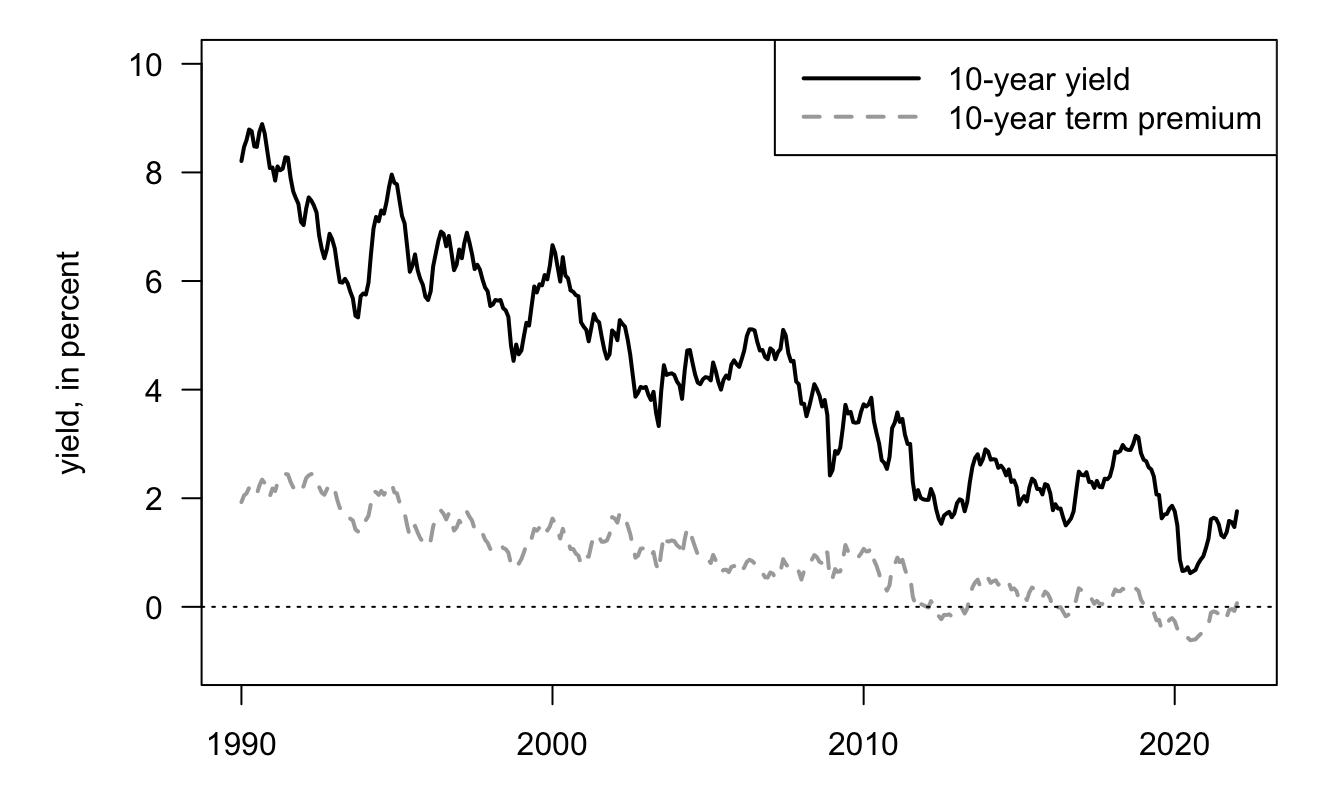
\includegraphics[width=0.95\linewidth]{TSM_files/figure-latex/fredKW-1} \caption{Kim and Wright (2005) outputs.}\label{fig:fredKW}
\end{figure}

\end{example}

\begin{example}[Ang and Piazzesi (2003)]
\protect\hypertarget{exm:AngPiazzesi}{}\label{exm:AngPiazzesi}

\citet{Ang_Piazzesi_2003} propose one of the first paper mixing latent and macrovariables. The set up is also of the form of \eqref{eq:GaussianVAR1}, except that the VAR features several lags.\footnote{Note that a VAR with \(p\) lags (i.e., a VAR(\(p\))) admits a VAR(1) companion form.} In their model, \(w_t = [f^{o}_{1,t},f^{o}_{2,t},f^{u}_{1,t},f^{u}_{2,t},f^{u}_{3,t}]'\) where:

\begin{itemize}
\tightlist
\item
  \(f^{o}_{1,t}\) is the first Principal Component of a set of 3 price indexes (growth rates)
\item
  \(f^{o}_{2,t}\) is the first Principal Component of a set of 4 real activity proxies (HELP, EMPLOY, IP, UE).
\item
  \(f^{u}_{i,t}\) are unobserved, or latent, factors.
\end{itemize}

The nominal short-term rate follows a Taylor rule. And latent factors are estimated via \emph{inversion techniques} (Subsection \ref{EstimationInversion}).

\begin{figure}

{\centering 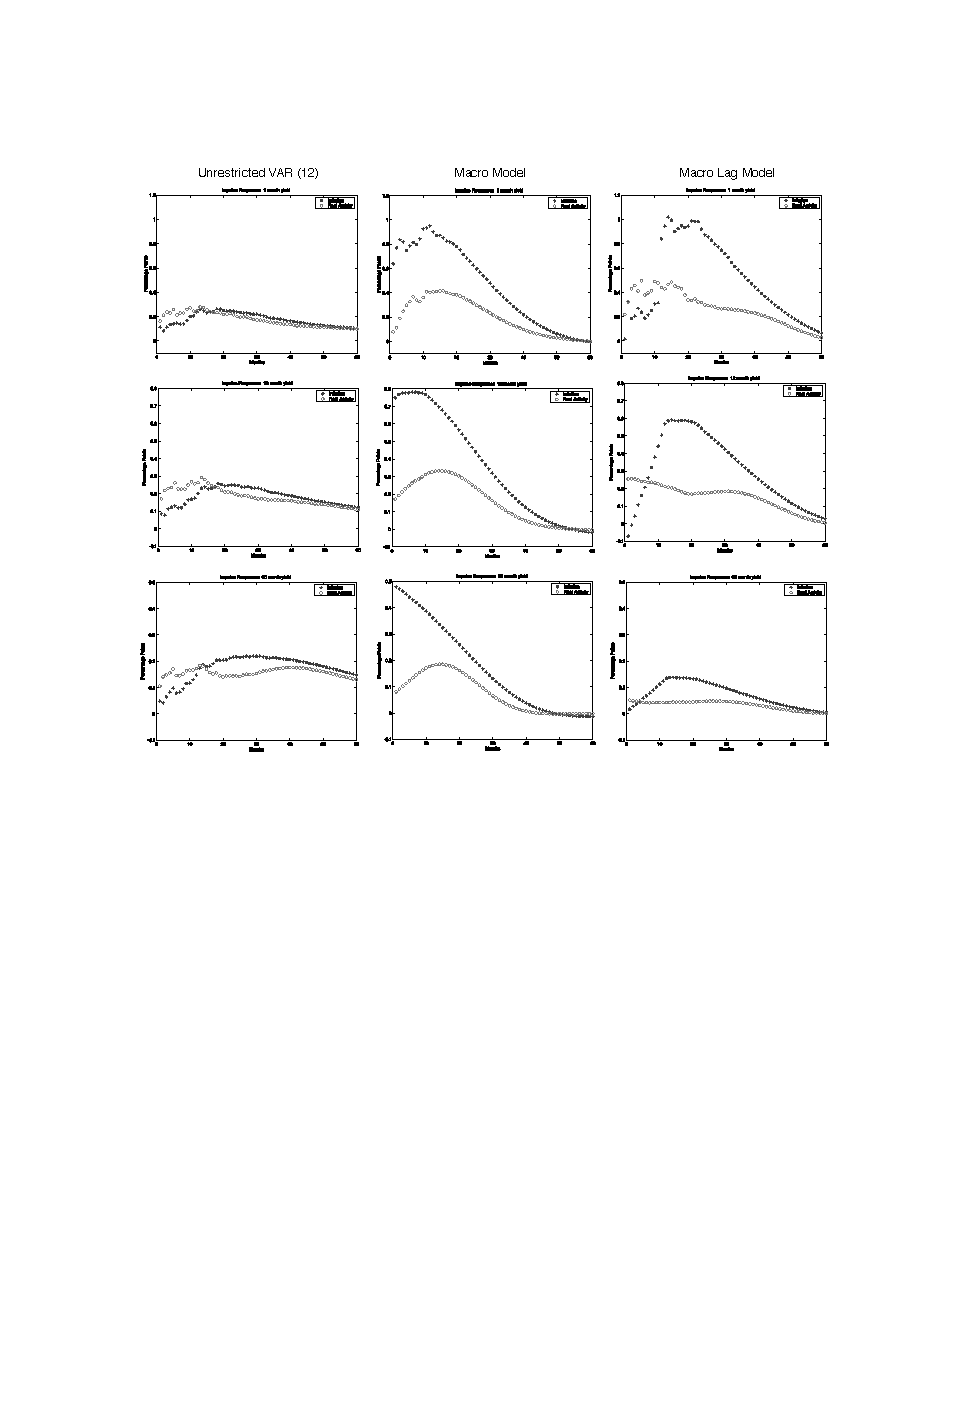
\includegraphics[width=0.95\linewidth]{figures/AngPiazzesi1} 

}

\caption{Source: Ang and Piazzesi (1998). Impulse response functions.}\label{fig:figAngPiazzesi}
\end{figure}

\end{example}

\begin{example}[Joslin, Priebsch and Singleton (2014)]
\protect\hypertarget{exm:JPS}{}\label{exm:JPS}

\citet{Joslin_Priebsch_Singleton_2014} first note that affine models stating that the short term rate is affine in macro factors imply that macro-factors are \emph{spanned} by the yield curve: macro-factors should be perfectly explained by yields of different maturities. Further, they show that this is not the case in the data. (That is, regressing macro factors on yields provides \(R^2\) that are far from one.)

They propose a model where macro factors are unspanned by the yield curve, but can still help predict yields. In their model, \(w_t = [\mathcal{P}_t',M_t']'\), where \(\mathcal{P}_t\) are yield factors (\(\approx\) principal components) and \(M_t\) are macro factors. The model is as follows:
\begin{eqnarray*}
i_t &=& \omega_{0} + \omega_{\mathcal{P}}'\mathcal{P}_t \\
\left[\begin{array}{c}\mathcal{P}_t \\ M_t \end{array}\right]
&=&
\left[\begin{array}{cc}\Phi_{\mathcal{P}\mathcal{P}}&\Phi_{\mathcal{P}M} \\
\Phi_{M\mathcal{P}}&\Phi_{MM} \end{array}\right]
\left[\begin{array}{c}\mathcal{P}_{t-1} \\ M_{t-1} \end{array}\right] + \Sigma \varepsilon_t \\
\left[\begin{array}{c}\mathcal{P}_t \\ M_t \end{array}\right] &=& \mu +
\left[\begin{array}{cc}\Phi^{\mathbb{Q}}_{\mathcal{P}\mathcal{P}}&{\color{red}0} \\
\Phi^{\mathbb{Q}}_{M\mathcal{P}}&\Phi^{\mathbb{Q}}_{MM} \end{array}\right]
\left[\begin{array}{c}\mathcal{P}_{t-1} \\ M_{t-1} \end{array}\right] + \Sigma \varepsilon^{\mathbb{Q}}_t,
\end{eqnarray*}
where \(\varepsilon_t\) and \(\varepsilon^{\mathbb{Q}}_t\) are \(\mathcal{N}(0,Id)\) under \(\mathbb{P}\) and \(\mathbb{Q}\), respectively.

\(M_t\) does not Granger-cause \(\mathcal{P}_t\) under \(\mathbb{Q}\). In other words, \(\mathcal{P}_t\) is exogenous under \(\mathbb{Q}\). And since \(i_t\) is affine in \(\mathcal{P}_t\) only (the loadings on \(M_t\) are null), it comes that the yield of any maturity \(i_{t,h}\) is affine in \(\mathcal{P}_t\) only (null loadings on \(M_t\)). However, since \(M_t\) does Granger-cause \(\mathcal{P}_t\) under \(\mathbb{P}\), the macro-shocks have dynamic effects on the yield curve. In other words, this model reconciles the facts that:

\begin{enumerate}
\def\labelenumi{\alph{enumi}.}
\tightlist
\item
  the level, slope and curvature explains the bulk of the variations of the yield curve,
\item
  macro factors affect yields,
\item
  the vectorial spaces spanned by yields on the one hand, and macroeconomic factors on the other hand do not coincide.
\end{enumerate}

\begin{figure}

{\centering 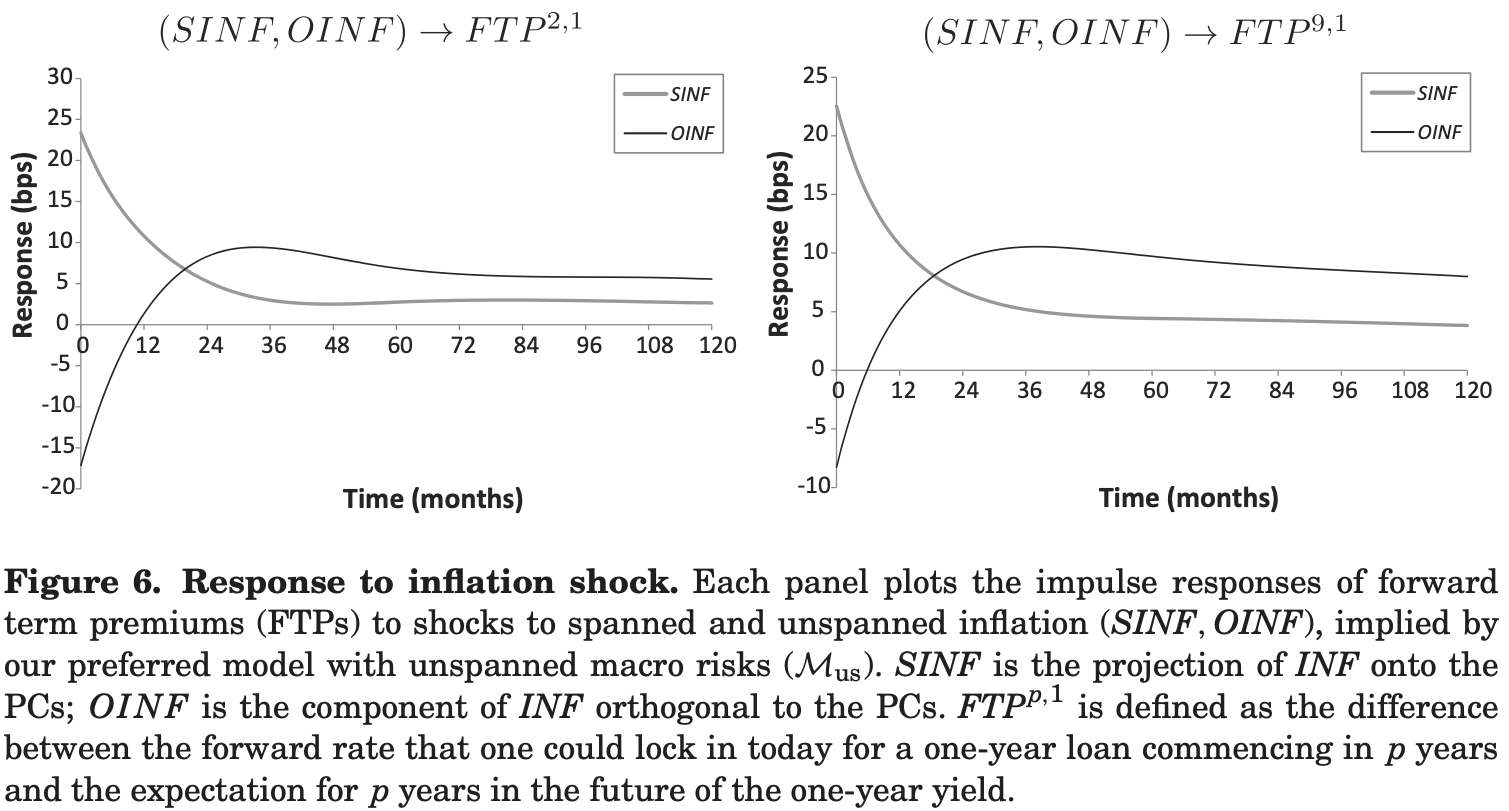
\includegraphics[width=0.95\linewidth]{figures/JPS_IRF} 

}

\caption{Source: Joslin, Priebsch, and Singleton (2014). Impulse response functions.}\label{fig:JPSIRF}
\end{figure}

\end{example}

\begin{example}[Ang, Boivin, Dong and Loo-Kung (2011)]
\protect\hypertarget{exm:Angetal2011}{}\label{exm:Angetal2011}

\citet{Ang_Boivin_Dong_LooKung_2011} propose a macro-finance model based on a quadratic framework. The short-term rate follows a Taylor rule with time-varying parameters:
\[
i_t = \omega_0 + a_t g_t + b_t \pi_t,
\]
where \(x_t=(g_t,\pi_t,a_t,b_t)'\) follows a Gaussian VAR. This is the context described in Example \ref{exm:QGVAR1}. The previous equation shows that \(r_t\) is linear in \(w_t = (x_t,vec(x_t x_t')')'\). Specifically:
\[
i_t = \omega_0 + \omega_1'w_t,
\]
with \(\omega_1 = [v,vec(V)]'\), where
\[
v = \left[
\begin{array}{c}
0\\
0\\
0\\
0
\end{array}
\right] \quad \mbox{and} \quad V = \left[
\begin{array}{cccc}
0 & 0& 1/2&0\\
0& 0& 0&1/2\\
1/2& 0& 0&0\\
0&1/2 &0 &0
\end{array}
\right].
\]

\begin{figure}

{\centering 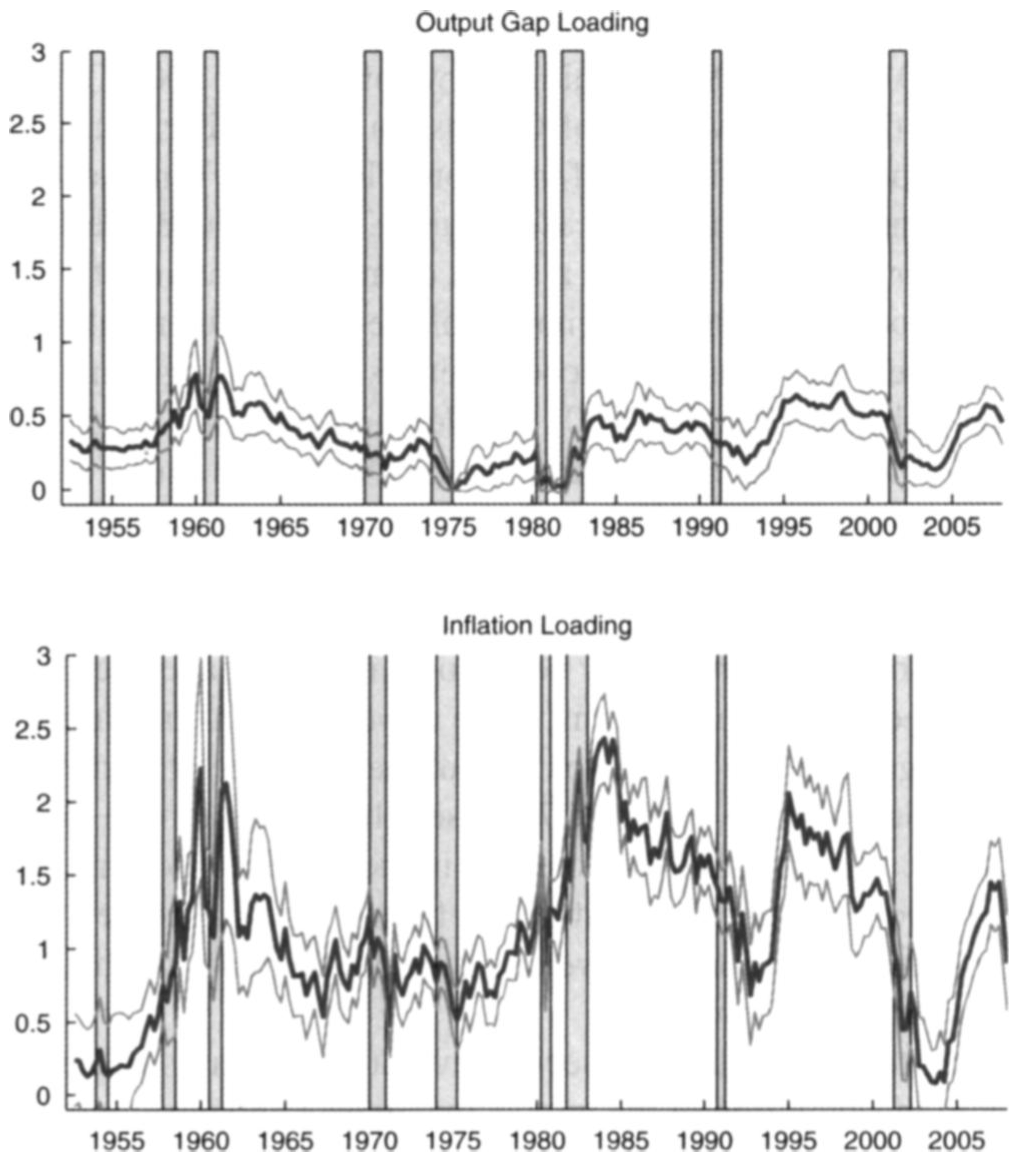
\includegraphics[width=0.7\linewidth]{figures/Ang_Boivin_loadings} 

}

\caption{Source: Ang, Boivin, Dong, Loo-Kung (2011). Estimated factor loadings ($a_t$ and $b_t$).}\label{fig:AngBoivin}
\end{figure}

\end{example}

\hypertarget{RiskFreeNonNegative}{%
\section{Non-Negative Affine Term Structure Model}\label{RiskFreeNonNegative}}

In the presence of physical currency, absence of arbitrage opportunity and of storing cost of cash, nominal interest rates should be nonnegative. Many standard models (e.g.~Gaussian ATSM) are non consistent with non-negative nominal yields. The period of extremely low interest rates challenged these models. Against this backdrop, approaches have been developed to accommodate zero (or effective) lower bounds. We provide two examples; only the second is an affine model.

\hypertarget{Shadowrate}{%
\subsection{The shadow-rate approach}\label{Shadowrate}}

The shadow-rate model is originally due to \citet{Black_1995}. In this model, the short term rate is given by:
\begin{equation}
i_t = \max(s_t,\underline{i}) = \underline{i} + \max(s_t-\underline{i},0),\label{eq:SRSTR}
\end{equation}
where \(s_t\) is the shadow short-term interest rate and \(\underline{i}\) is the effective lower bound (\(\le 0\)). While \(s_t\) can be real-valued, the short term rate is nonnegative under \eqref{eq:SRSTR}. In shadow-rate models, the shadow rate \(s_t\) is usually a linear combination of a vector \(w_t\) that follows a Gaussian auto-regressive model. While \(s_t\) is a linear combination of components of an affine process, this is not the case for \(i_t\). As a result, pricing formula are not available in closed-form. Approximation formula have been proposed by, e.g., \citet{Krippner_2013}, \citet{Priebsch_2013}, \citet{Wu_Xia_2016}.

Let us describe the latter approach \citep{Wu_Xia_2016}. As in Subsection \ref{RiskFreeGaussian}, the SDF is defined as:
\[
\mathcal{M}_{t,t+1} = \exp(- i_t + \alpha_t'w_{t+1} - \psi_t(\alpha_t)), \mbox{ where } \alpha_t = \alpha_0 + \alpha_1'w_t,
\]
(this is Eq. \eqref{eq:keySDF}), but the short-term rate \(i_t\) is given by \(i_t = \max(s_t,0)\), with
\[
s_t = \delta_0 + \delta_1' w_t.
\]
The shadow rate \(s_t\) is part of a state vector \(w_t\) that follows a Gaussian VAR, as in \eqref{eq:GaussianVAR1} (or \(s_t\) can be a linear combination of components of \(w_t\)). As before, the \(\mathbb{Q}\)-dynamics of \(w_t\) is also a Gaussian VAR, as in \eqref{eq:GaussianQdyn}. (Indeed, using the previous specification of the SDF, the non-linear \(i_t\) term vanishes in the Radon-Nikodym derivatives; see Eq. \eqref{eq:RadonNikodym}.)

The price of a nominal zero-coupon bond is still given by \eqref{eq:ihandM}, that is:
\[
B_{t,h} = \mathbb{E}^{\mathbb{Q}}_t \exp(-i_t--i_{t+1}-\dots-i_{t+h-1});
\]
but this price is not exponential affine in \(s_t\) because of the max operator relating \(i_t\) to \(s_t\) (see Eq. \eqref{eq:SRSTR}). As a result, we can no longer exploit the tractable calculation of the multi-horizon Laplace transform of \(w_t\) to price this bond.

The approximation approach proposed by \citet{Wu_Xia_2016} is based on an approximation to the conditional expectations of forward rates. Using the results of Subsection \ref{FWD}, we have (Eq. \eqref{eq:forward}):
\[
f_{n-1,n,t} = n i_{t,n} - (n-1) i_{t,n-1}.,
\]
for \(n>0\) (and using \(i_{t,0}=0\), i.e., \(f_{0,1,t}=i_t\)). Equivalently, for \(h>0\):
\[
i_{t,h} =  \frac{1}{h}(f_{t,0,1}+f_{t,1,2}+\dots+f_{t,h-1,h}).
\]

The approximation of \citet{Wu_Xia_2016} consists in finding approximations of the forward rates \(f_{t,n-1,n}\) (denoted by \(\tilde{f}_{t,n-1,n}\), say) and to use them in the previous equation to get:
\begin{equation}
i_{t,h} \approx  \frac{1}{h}\left(\tilde{f}_{t,0,1}+\tilde{f}_{t,1,2}+\dots+\tilde{f}_{t,h-1,h}\right).\label{eq:RapproxSR}
\end{equation}

Using that, for any random variable \(Z\), we have \(\log(\mathbb{E}[e^Z]) \approx \mathbb{E}[Z] + \frac{1}{2} \mathbb{V}ar[Z]\) (based on a second-order Taylor expansion of the log-Laplace transform), \citet{Wu_Xia_2016} further show that:
\begin{eqnarray}
f_{t,n,n+1} &=& -\log\left(\mathbb{E}_t^{\mathbb{Q}}\left(e^{-\sum_{j=0}^n i_{t+j}}\right)\right) + \log\left(\mathbb{E}_t^{\mathbb{Q}}\left(e^{-\sum_{j=0}^{n-1} i_{t+j}}\right)\right)\\
&\approx& \mathbb{E}_t^{\mathbb{Q}}[i_{t+n}] - \frac{1}{2}\left(\mathbb{V}ar_t^{\mathbb{Q}}\left(\sum_{j=0}^n i_{t+j}\right)-\mathbb{V}ar_t^{\mathbb{Q}}\left(\sum_{j=0}^{n-1} i_{t+j}\right)\right).
\end{eqnarray}

The expectation can be computed analytically. Using \eqref{eq:SRSTR}, it is indeed of the form \(\underline{i} + \mathbb{E}_t^{\mathbb{Q}}[ \max(s_{t+n}-\underline{i},0)]\), where
\[
s_{t+n}-\underline{i}|\underline{w_t} \sim \mathcal{N}\left(\bar{a}_n+b_n'w_t- \underline{i},\sigma_n^{\mathbb{Q}}\right),
\]
with
\[
\bar{a}_n = \delta_0 + \delta_1'\left(\sum_{j=0}^{n-1} \left[\Phi^{\mathbb{Q}}\right]^j\right)\mu^{\mathbb{Q}}, \quad \mbox{and} \quad b_n' = \delta_1'\left(\Phi^{\mathbb{Q}}\right)^n,
\]
and
\[
\sigma_n^{\mathbb{Q}} := \mathbb{V}ar^{\mathbb{Q}}_t\left(s_{t+n}\right)= \delta_1'\left(\sum_{j=0}^{n-1} \left[\Phi^{\mathbb{Q}}\right]^j\right)\Sigma \Sigma' \left(\sum_{j=0}^{n-1} \left[\Phi^{\mathbb{Q}}\right]^j\right)'\delta_1.
\]

Hence, using standard results on the truncated normal distribution (see Figure \ref{fig:Mills}),\footnote{If \(X\sim \mathcal{N}(\mu,\sigma^2)\), then \(\mathbb{E}(\max(X,0))=\sigma g\left(\frac{\mu}{\sigma}\right)= \mu\Phi\left(\frac{\mu}{\sigma}\right)+\sigma\phi\left(\frac{\mu}{\sigma}\right)\).} they obtain:
\[
\mathbb{E}_t^{\mathbb{Q}}[i_{t+n}] = \underline{i} + \sigma_n^{\mathbb{Q}}g\left(\frac{\bar{a}_n + b_n'X_t - \underline{i}}{\sigma_n^{\mathbb{Q}}}\right),
\]
where \(g(x)= x\Phi(x)+\phi(x)\), \(\Phi\) and \(\phi\) being the c.d.f. and p.d.f. of the standard normal distribution, respectively.

They also show that
\[
\frac{1}{2}\left(\mathbb{V}ar_t^{\mathbb{Q}}\left(\sum_{j=0}^n i_{t+j}\right)-\mathbb{V}ar_t^{\mathbb{Q}}\left(\sum_{j=0}^{n-1} i_{t+j}\right)\right) \approx \Phi\left(\frac{\bar{a}_n + b_n'X_t - \underline{i}}{\sigma_n^{\mathbb{Q}}}\right)\times(\bar{a}_n - a_n),
\]
where \(a_n = \bar{a}_n - \frac{1}{2}\sigma_n^{\mathbb{Q}}\). They finally obtain:
\[
\boxed{f_{t,n,n+1} \approx \tilde{f}_{t,n,n+1} = \underline{i} + \sigma_n^{\mathbb{Q}}g\left(\frac{a_n + b_n'X_t - \underline{i}}{\sigma_n^{\mathbb{Q}}}\right),}
\]
which is used in \eqref{eq:RapproxSR} to obtain an approximation to \(i_{t,h}\).

In the following code, we simulate a shadow-rate path and compute the term structure of the approximated forward rates \(f_{t,n,n+1}\) and the resulting nominal rates \(i_{t,h}\) for the date indicated by the vertical grey line in the upper plot.

\begin{Shaded}
\begin{Highlighting}[]
\FunctionTok{library}\NormalTok{(TSModels)}
\CommentTok{\# Specify model:}
\NormalTok{n }\OtherTok{\textless{}{-}} \DecValTok{2} \CommentTok{\# number of factors}
\NormalTok{rho }\OtherTok{\textless{}{-}} \FunctionTok{matrix}\NormalTok{(}\DecValTok{0}\NormalTok{,n,n)}
\FunctionTok{diag}\NormalTok{(rho) }\OtherTok{\textless{}{-}}\NormalTok{ .}\DecValTok{97}
\NormalTok{mu }\OtherTok{\textless{}{-}} \FunctionTok{matrix}\NormalTok{(}\DecValTok{0}\NormalTok{,n,}\DecValTok{1}\NormalTok{)}
\NormalTok{Sigma }\OtherTok{\textless{}{-}} \FunctionTok{diag}\NormalTok{(n)}
\NormalTok{delta}\FloatTok{.0} \OtherTok{\textless{}{-}} \DecValTok{0}\NormalTok{;delta}\FloatTok{.1} \OtherTok{\textless{}{-}} \FunctionTok{rep}\NormalTok{(.}\DecValTok{01}\NormalTok{,n)}
\NormalTok{r.bar }\OtherTok{\textless{}{-}} \DecValTok{0} \CommentTok{\# r = max(s,r.bar) [i.e., r.bar=0 in standard model]}
\NormalTok{Model }\OtherTok{\textless{}{-}} \FunctionTok{list}\NormalTok{(}\AttributeTok{rho =}\NormalTok{ rho,}\AttributeTok{mu =}\NormalTok{ mu,}\AttributeTok{Sigma =}\NormalTok{ Sigma,}
              \AttributeTok{delta.0 =}\NormalTok{ delta}\FloatTok{.0}\NormalTok{,}\AttributeTok{delta.1 =}\NormalTok{ delta}\FloatTok{.1}\NormalTok{,}\AttributeTok{r.bar =}\NormalTok{ r.bar)}
\CommentTok{\# Simulate model and compute shadow rate:}
\NormalTok{X }\OtherTok{\textless{}{-}} \FunctionTok{simul.var}\NormalTok{(Model,}\AttributeTok{nb.sim =} \DecValTok{200}\NormalTok{) }\CommentTok{\# simulated path}
\NormalTok{s }\OtherTok{\textless{}{-}}\NormalTok{ delta}\FloatTok{.0} \SpecialCharTok{+}\NormalTok{ X }\SpecialCharTok{\%*\%}\NormalTok{ delta}\FloatTok{.1}
\CommentTok{\# Compute yields:}
\NormalTok{res }\OtherTok{\textless{}{-}} \FunctionTok{compute.price.WX}\NormalTok{(Model,X,}\AttributeTok{max.H=}\DecValTok{100}\NormalTok{)}
\CommentTok{\# Prepare plots:}
\FunctionTok{par}\NormalTok{(}\AttributeTok{plt=}\FunctionTok{c}\NormalTok{(.}\DecValTok{1}\NormalTok{,.}\DecValTok{95}\NormalTok{,.}\DecValTok{2}\NormalTok{,.}\DecValTok{75}\NormalTok{))}
\FunctionTok{par}\NormalTok{(}\AttributeTok{mfrow=}\FunctionTok{c}\NormalTok{(}\DecValTok{2}\NormalTok{,}\DecValTok{1}\NormalTok{))}
\FunctionTok{plot}\NormalTok{(s,}\AttributeTok{type=}\StringTok{"l"}\NormalTok{,}\AttributeTok{xlab=}\StringTok{"time"}\NormalTok{,}\AttributeTok{ylab=}\StringTok{""}\NormalTok{,}\AttributeTok{lwd=}\DecValTok{2}\NormalTok{,}\AttributeTok{main=}\StringTok{"(a) Shadow rate"}\NormalTok{)}
\NormalTok{t }\OtherTok{\textless{}{-}} \DecValTok{50} \CommentTok{\#t \textless{}{-} which(s==min(s))}
\FunctionTok{abline}\NormalTok{(}\AttributeTok{v=}\NormalTok{t,}\AttributeTok{col=}\StringTok{"dark grey"}\NormalTok{,}\AttributeTok{lwd=}\DecValTok{2}\NormalTok{,}\AttributeTok{lty=}\DecValTok{3}\NormalTok{)}
\FunctionTok{plot}\NormalTok{(res}\SpecialCharTok{$}\NormalTok{vec.f[t,],}\AttributeTok{type=}\StringTok{"l"}\NormalTok{,}\AttributeTok{xlab=}\StringTok{"maturity"}\NormalTok{,}\AttributeTok{ylab=}\StringTok{""}\NormalTok{,}
     \AttributeTok{lwd=}\DecValTok{2}\NormalTok{,}\AttributeTok{main=}\StringTok{"(b) yields and forward rates"}\NormalTok{)}
\FunctionTok{lines}\NormalTok{(res}\SpecialCharTok{$}\NormalTok{vec.y[t,],}\AttributeTok{col=}\StringTok{"red"}\NormalTok{,}\AttributeTok{lwd=}\DecValTok{2}\NormalTok{)}
\FunctionTok{legend}\NormalTok{(}\StringTok{"topright"}\NormalTok{, }
       \FunctionTok{c}\NormalTok{(}\StringTok{"forward rates"}\NormalTok{,}\StringTok{"yields to maturity"}\NormalTok{),}\AttributeTok{lwd=}\FunctionTok{c}\NormalTok{(}\DecValTok{2}\NormalTok{),}\AttributeTok{lty=}\DecValTok{1}\NormalTok{,}
       \AttributeTok{col=}\FunctionTok{c}\NormalTok{(}\StringTok{"black"}\NormalTok{,}\StringTok{"red"}\NormalTok{),}\AttributeTok{bg =} \StringTok{"white"}\NormalTok{)}
\end{Highlighting}
\end{Shaded}

\begin{figure}

{\centering 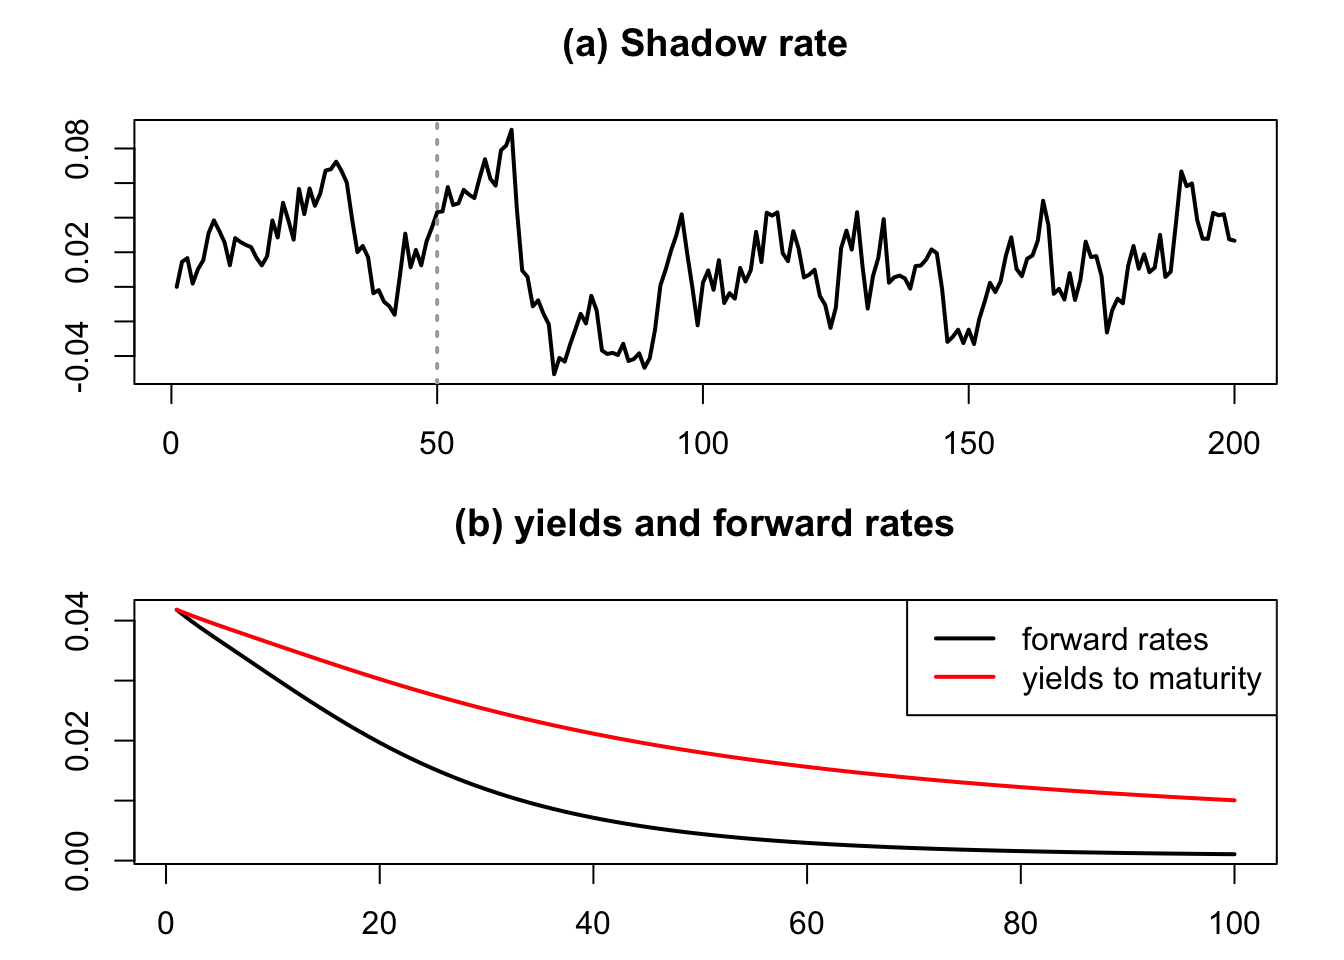
\includegraphics[width=0.95\linewidth]{TSM_files/figure-latex/WuXia-1} 

}

\caption{The upper plot shows a simulated path of the shadow rate $s_t$. The bottom plot shows the approximated forward rate $f_{t,n,n+1}$ and the resulting nominal rates $i_{t,h}$ for the date indicated by the vertical grey line in the upper plot.}\label{fig:WuXia}
\end{figure}

\begin{figure}

{\centering 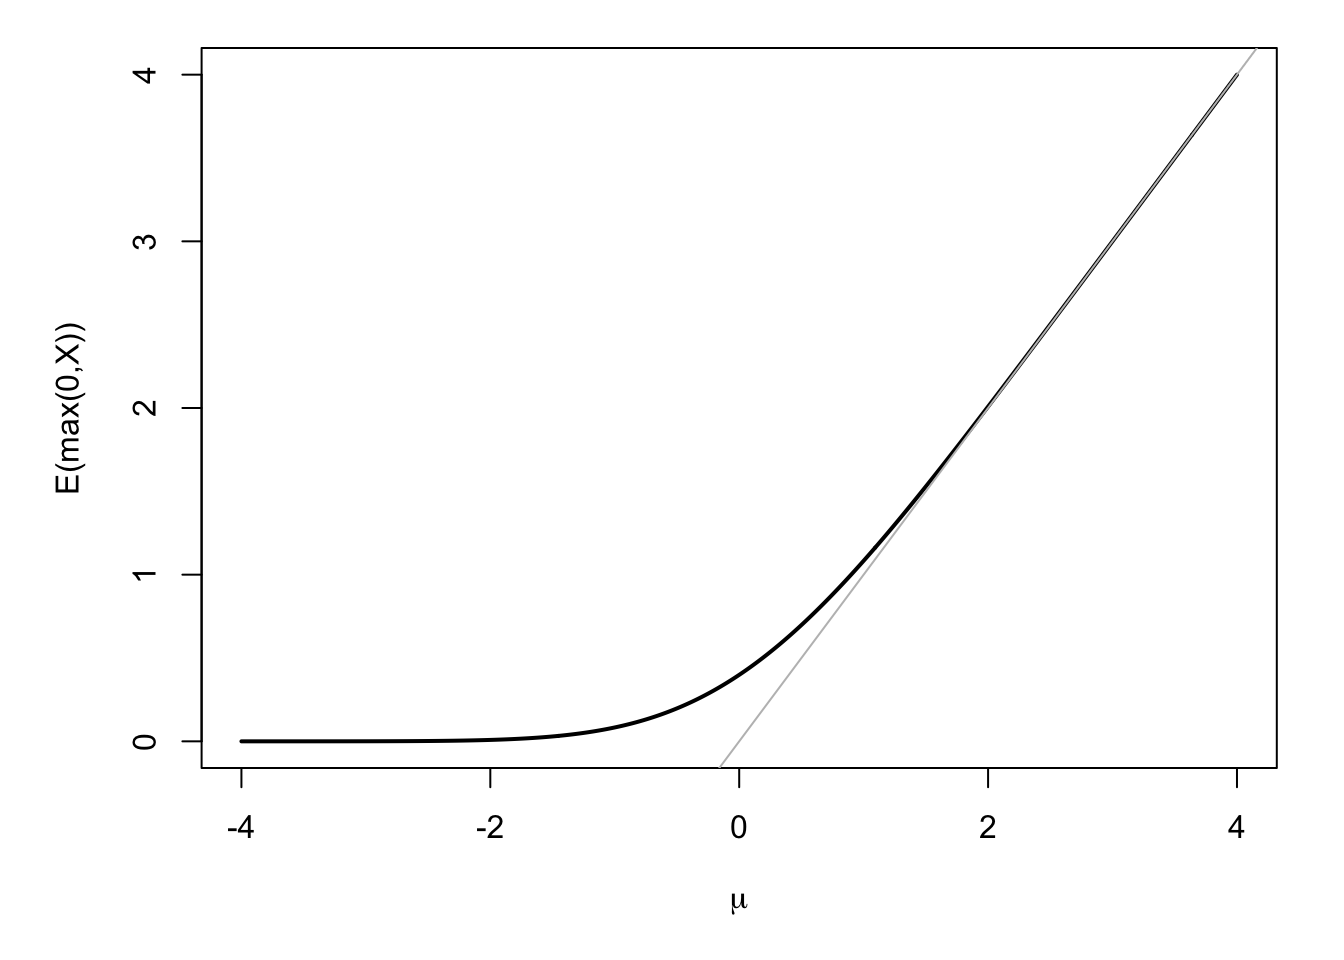
\includegraphics[width=0.95\linewidth]{TSM_files/figure-latex/Mills-1} 

}

\caption{This figure shows $\mathbb{E}(\max(0,X))$ for $X \sim \mathcal{N}(\mu,1)$, as a function of $\mu$. More generally, if $X\sim \mathcal{N}(\mu,\sigma^2)$, then $\mathbb{E}(\max(X,0))=\sigma g\left(\frac{\mu}{\sigma}\right)= \mu\Phi\left(\frac{\mu}{\sigma}\right)+\sigma\phi\left(\frac{\mu}{\sigma}\right)$, where $\Phi$ and $\phi$ are the c.d.f. and p.d.f. of the standard normal distirbution, respectively.}\label{fig:Mills}
\end{figure}

\hypertarget{the-auto-regressive-gamma-approach}{%
\subsection{The auto-regressive gamma approach}\label{the-auto-regressive-gamma-approach}}

\citet{zarg_2017} introduce an affine framework where the short-term rate can stay at zero for a prolonged period of time and with a stochastic lift-off probability.

Under \(\mathbb{P}\) and \(\mathbb{Q}\), the state vector \(w_t\) follows a multi-variate auto-regressive gamma (VARG) process---a multivariate extension of Example \ref{exm:ARG1}. Conditionally on \(\underline{w_t}\), the \(n\) components of \(w_{t+1}\) are independent and distributed as follows:
\begin{equation}
\frac{w_{i,t+1}}{\mu_i} \sim \gamma(\nu_i+z_{i,t}) \quad \mbox{where} \quad z_{i,t} \sim {\mathcal P} \left( \alpha_i + \beta_i' w_t \right).\label{eq:VARG}
\end{equation}
If \(\mu = (\mu_1,\dots,\mu_n)'\), \(\alpha = (\alpha_1,\dots,\alpha_n)'\), \(\nu = (\nu_1,\dots,\nu_n)'\) and \(\beta = (\beta_1,\dots,\beta_n)\), then
\begin{eqnarray*}
\varphi_t(u) &=& \exp\left[\left(\frac{u \odot \mu}{1 - u \odot \mu}\right)'\beta' w_t \right.\\
&& \left. + \alpha'\left(\frac{u \odot \mu}{1 - u \odot \mu}\right) - \nu'\log(1 - u \odot \mu)\right],
\end{eqnarray*}
where \(\odot\) denotes the element-by-element multiplication and, where, with abuse of notation, the division and log operators work element-by-element when applied to vectors.

In their baseline model, \citet{zarg_2017} use four factors. They set \(\nu_1 = \nu_2 = 0\), implying that \(w_{1,t}\) and \(w_{2,t}\) can stay at zero (see Example \ref{exm:ARG1}). The short-term rate \(i_t\) is posited to be an affine combination of \(w_{1,t}\) and \(w_{2,t}\), that is:
\[
i_t = \omega'w_t = \omega_{1} w_{1,t} + \omega_{2} w_{2,t},
\]
hence, it can stay at zero.

Factors \(w_{3,t}\) and \(w_{4,t}\) Granger-cause \(w_{1,t}\) and \(w_{2,t}\), thereby causing \(i_t\). As a result, for \(h \ge 2\), \(i_{t,h}\) is a non-zero combination of the four components of \(w_t\).

For the same reason, when \(i_t=0\), the lift-off probability depends on \(w_{3,t}\) and \(w_{4,t}\). The framework offers closed-form solutions for lift-off probabilities. Indeed, using Lemma \ref{lem:lemPetitLemme}:
\[
\mathbb{P}_t(\alpha'w_{t+h}=0) = \lim_{u \rightarrow -\infty} \varphi_{t,h}(0,\dots,0,u\alpha),
\]
where \(\varphi_{t,h}\) is the multi-horizon Laplace transform defined in \eqref{eq:multiLT}, which can be computed using Proposition \ref{prp:reverseMLT}. We have:
\begin{equation}
\left\{
\begin{array}{l}
\mathbb{P}_t(i_{t+h}>0) = 1 - \lim_{u \rightarrow -\infty} \varphi_{t,h}(0,\dots,0,u\omega) \\ \\
\mathbb{P}_t(i_{t+1}=0,\dots,i_{t+h}=0) = \lim_{u \rightarrow -\infty} \varphi_{t,h}(u\omega,\dots,u\omega,u\omega) \equiv p_{h}\\ \\
\mathbb{P}_t(i_{t+1}=0,\dots,i_{t+h-1}=0,i_{t+h}>0) = p_{h-1} - p_h.
\end{array}
\right.
\end{equation}
Other lift-off probabilities, of the type \(\mathbb{P}_t[i_{t+h,k}>threshold]\), can be derived from \eqref{eq:DPS}.

\citet{zarg_2017} esitmate this model by means of Kalman filtering techniques (see Subsection \ref{KalmanQML}). Observed variables include (levels of) yields, as well as survey-based forecasts of yields (see Subsection \ref{EstimationPersistency} and (e-GARCH-based) proxies of conditional variances (see Eq. \eqref{eq:condvar}).

\begin{figure}

{\centering 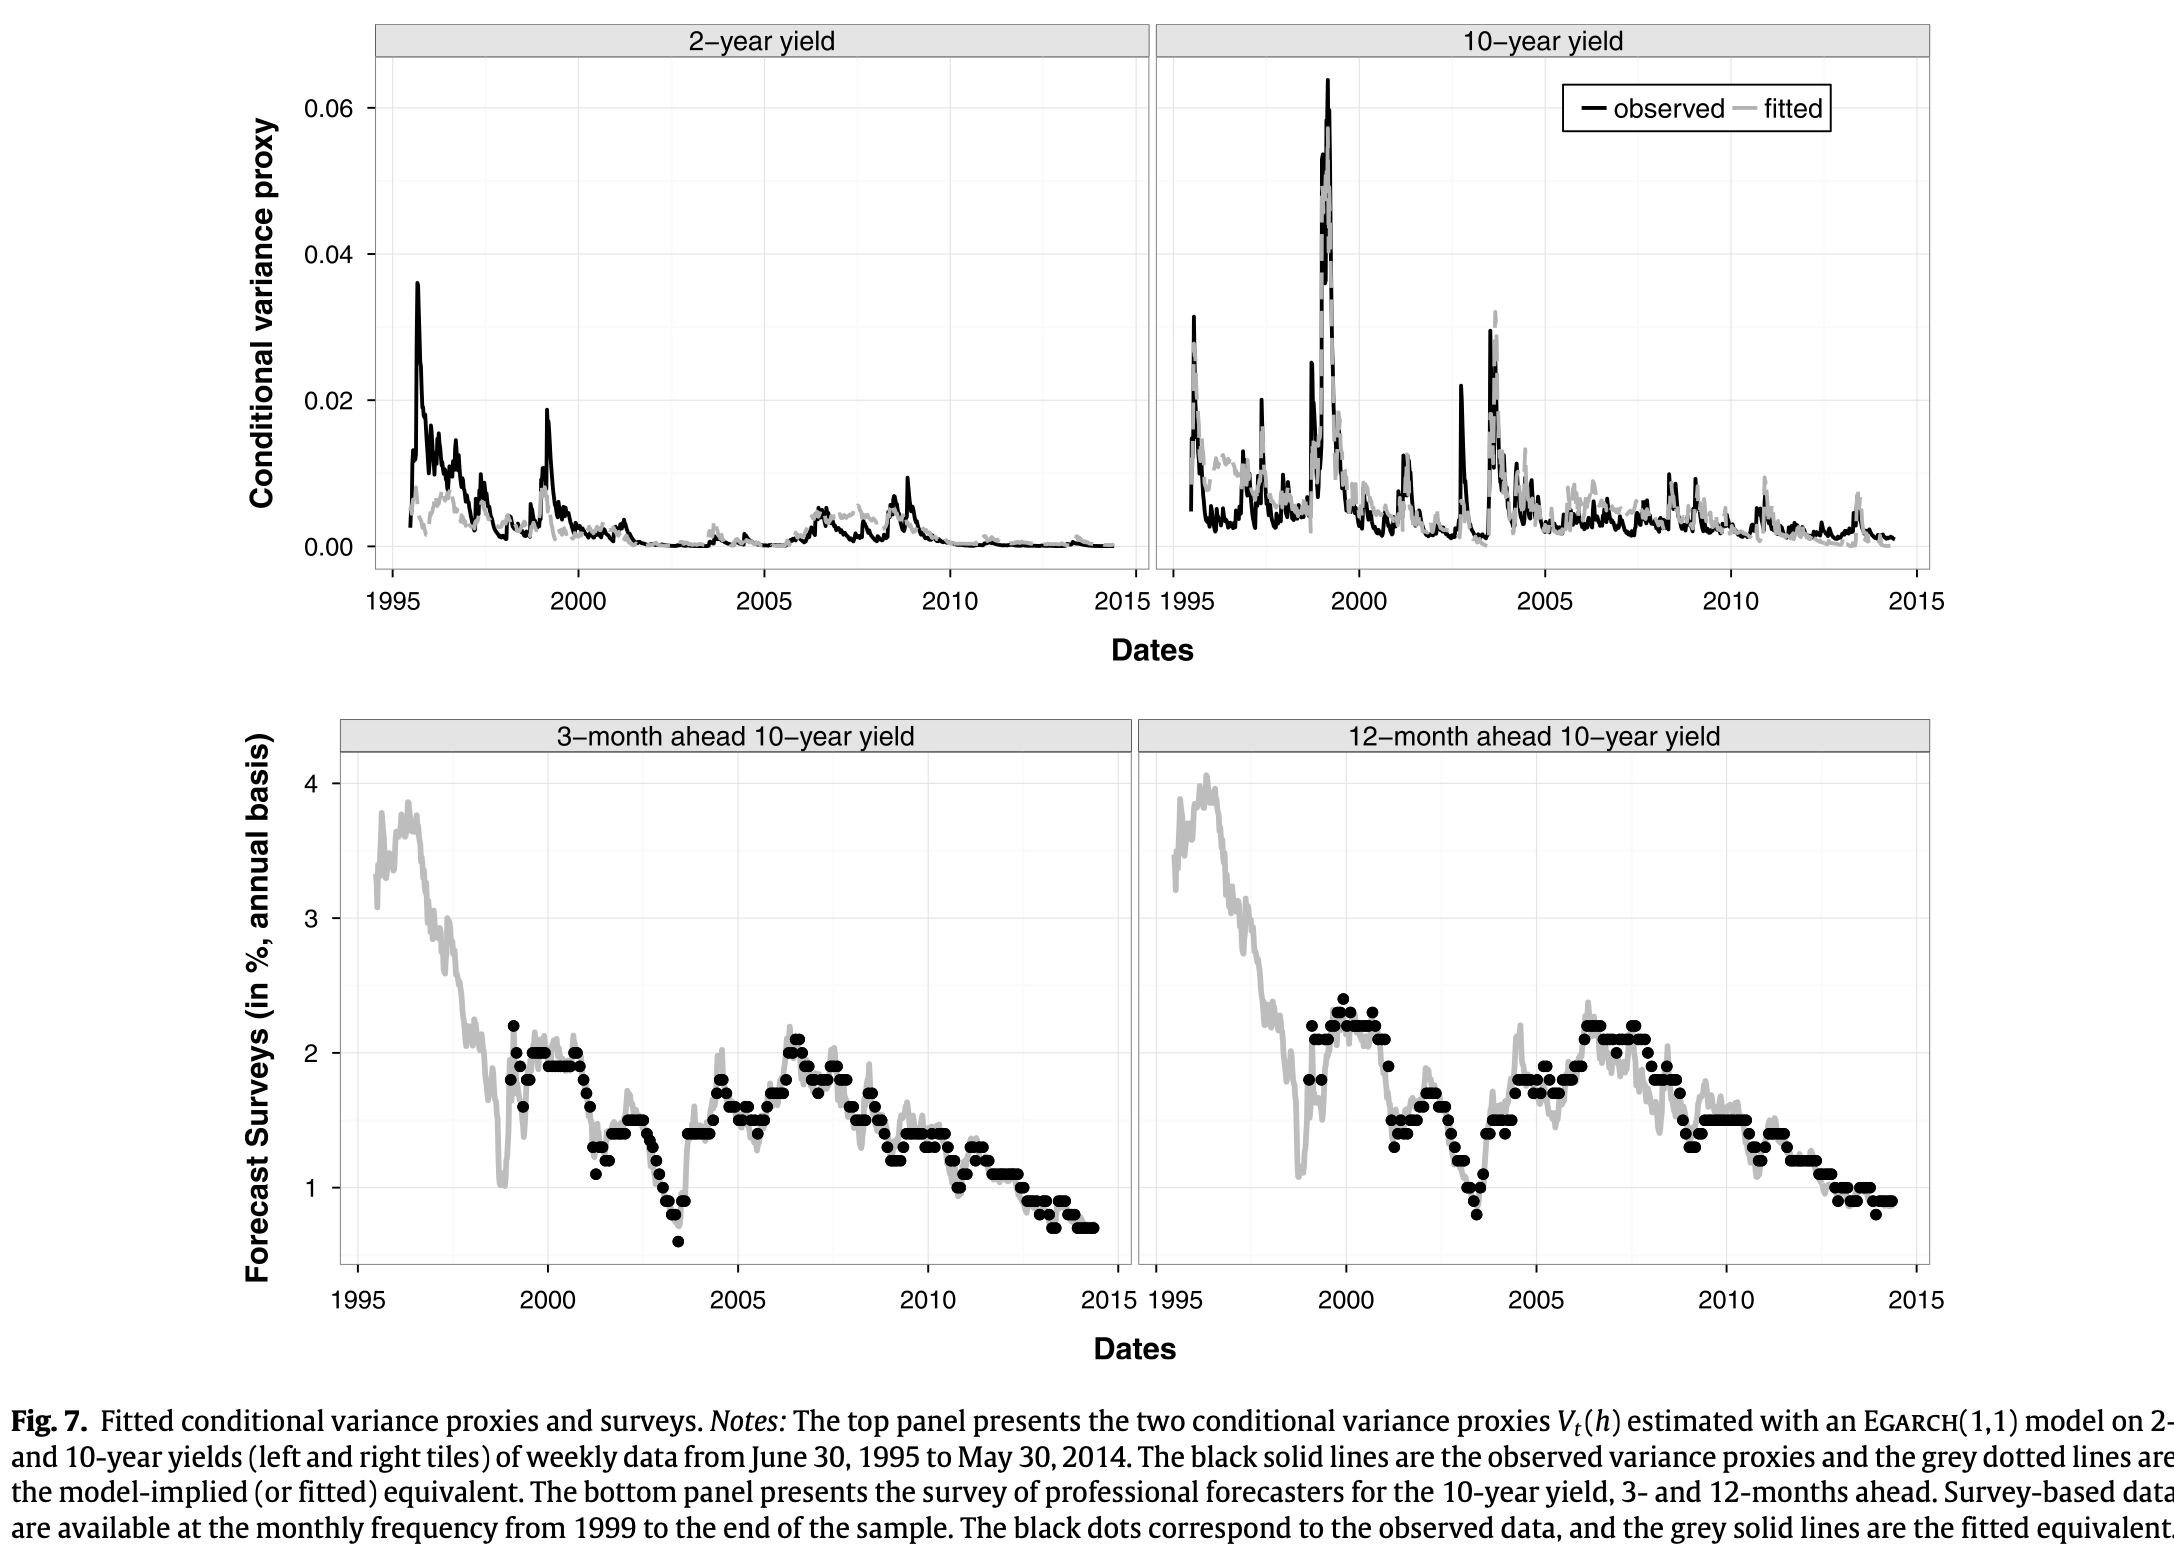
\includegraphics[width=0.95\linewidth]{figures/Figure_fit_ZARG} 

}

\caption{Source: Monfort et al. (2017). Model fit of conditional variances and surveys of professional forecasters.}\label{fig:fitZarg}
\end{figure}

\begin{figure}

{\centering 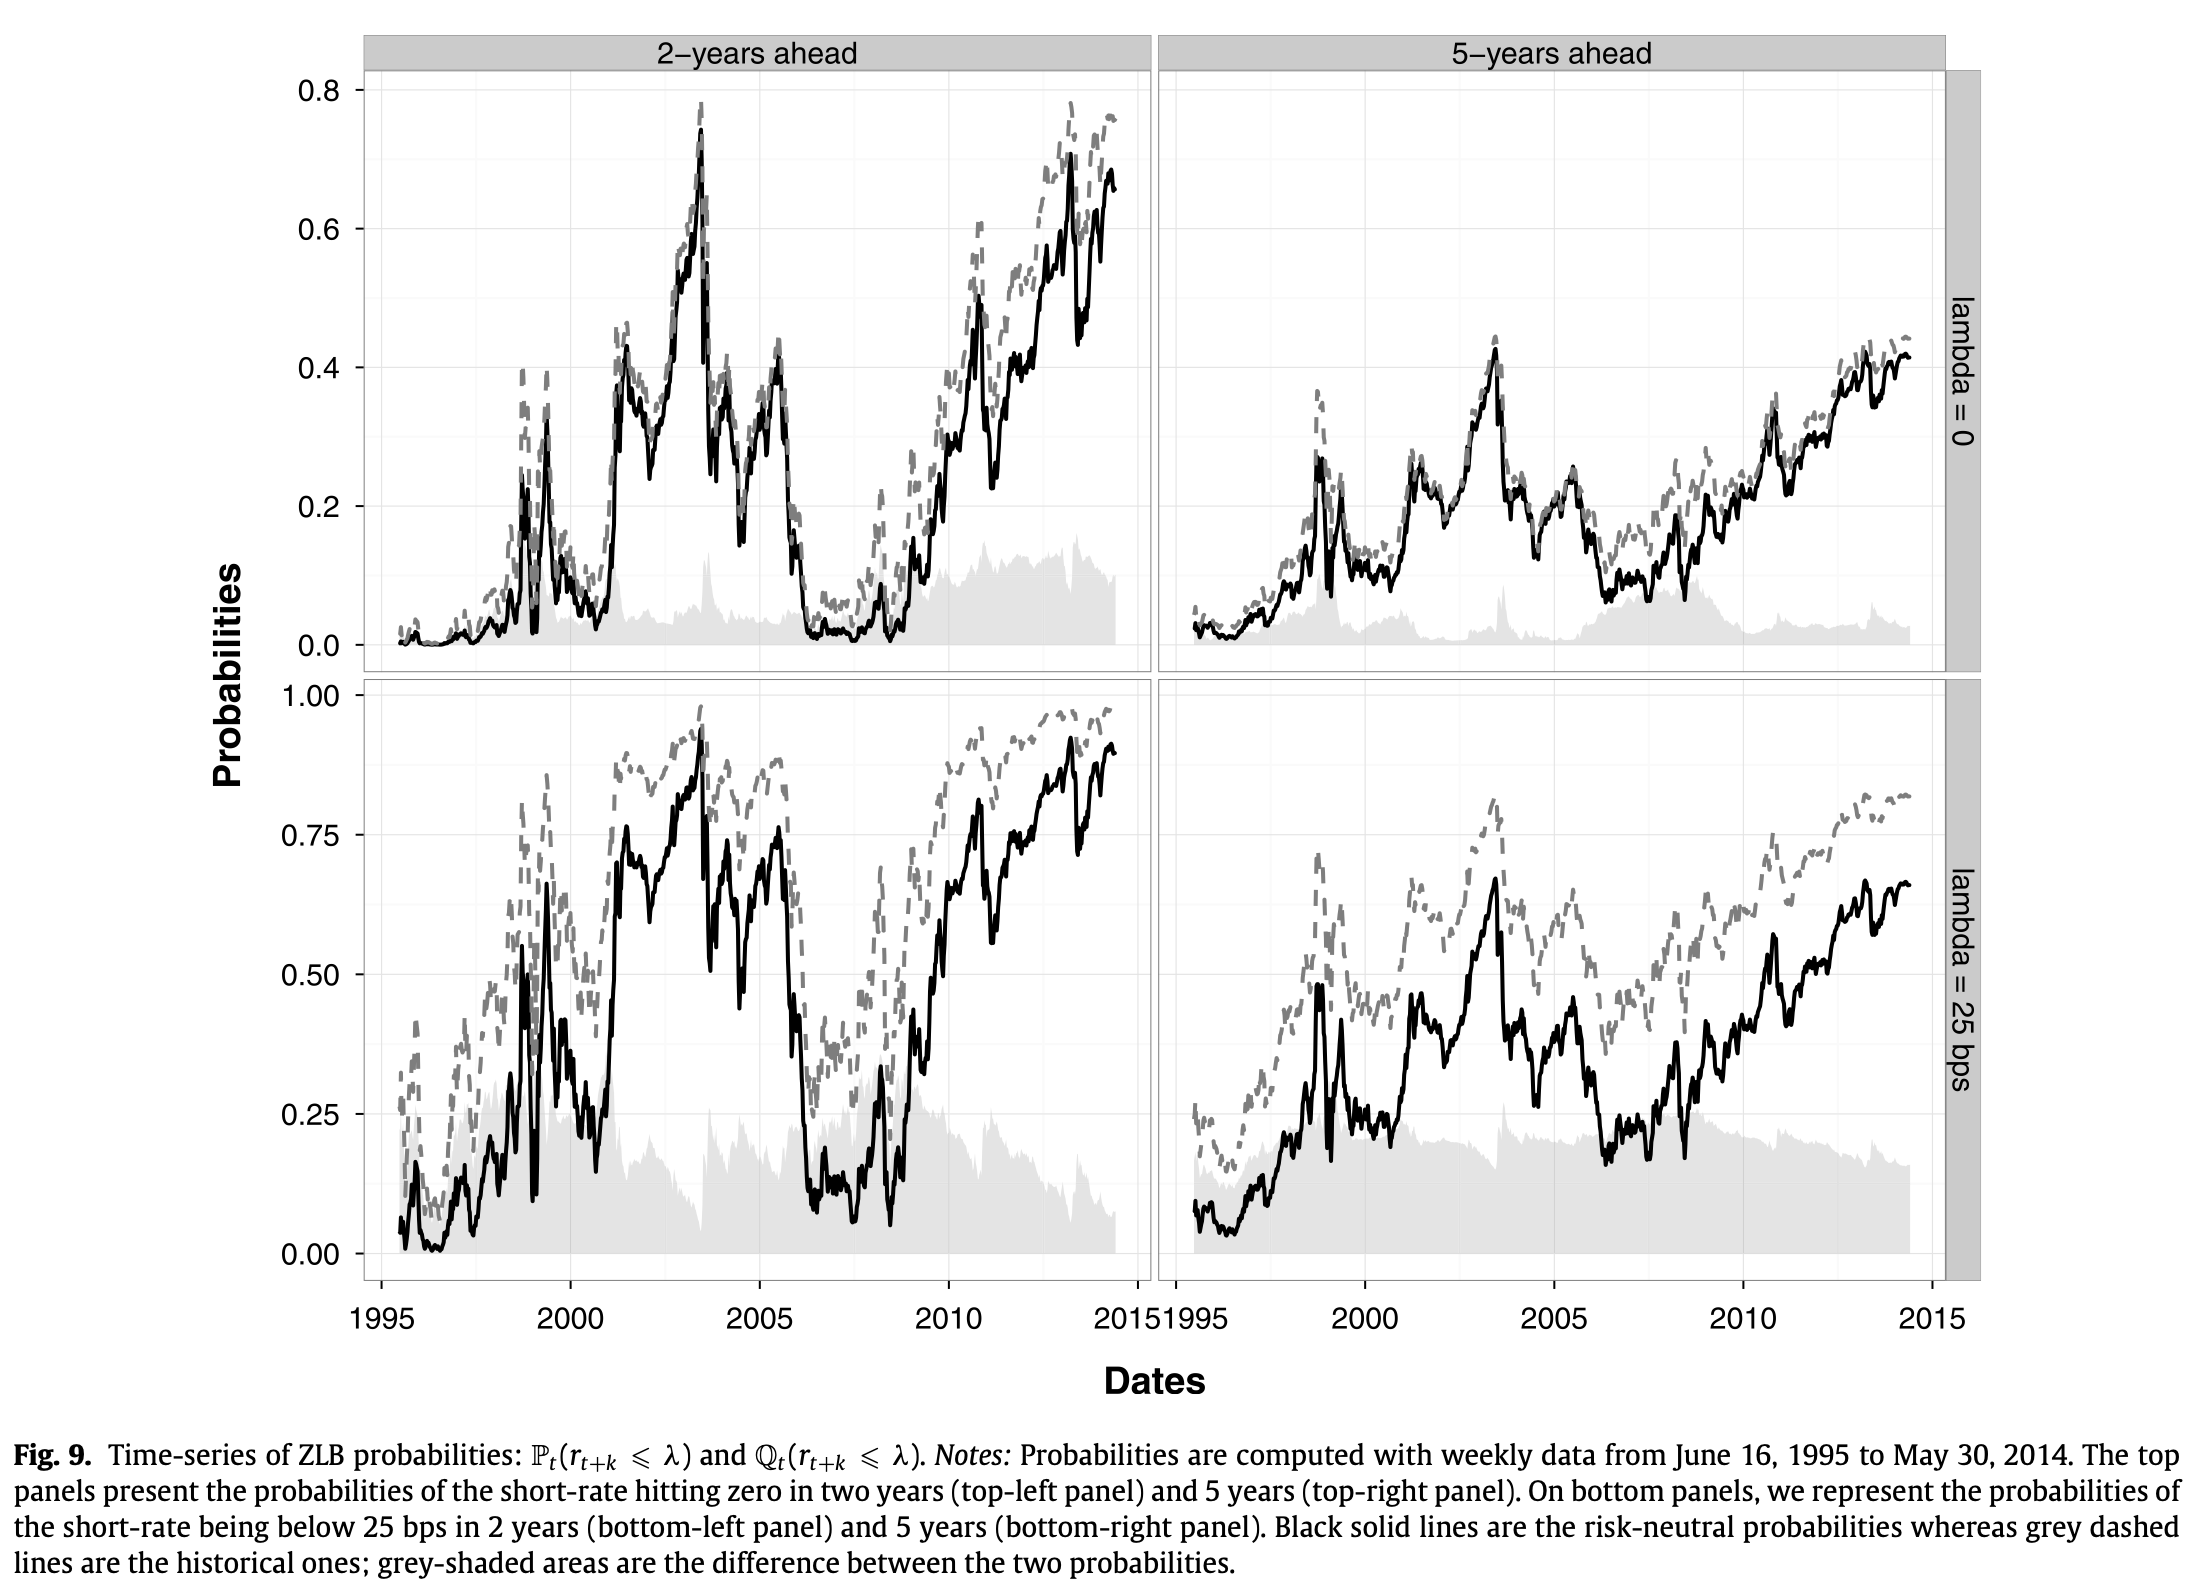
\includegraphics[width=0.95\linewidth]{figures/Figure_LiftOff} 

}

\caption{Source: Monfort et al. (2017). Lift-off probabilities.}\label{fig:liftOff}
\end{figure}

\hypertarget{constructing}{%
\section{Appendix -- Constructing the yield curve}\label{constructing}}

Interest rates are observed on financial markets. There are two broad categories of interest rate: those associate with bonds and those associated with derivatives (swaps, see Subsection \ref{Swaps}). For each category, there are, in turn, different types of yield curves:

\begin{itemize}
\tightlist
\item
  \textbf{Bonds}: yields-to-maturity, par yields, zero-coupon yields. Besides, even for a given issuer, there may be different yield curves if this issuer has issued different types of bonds in the past (e.g., nominal, inflation-indexed, green).
\item
  \textbf{Swaps}: there is one swap curve per reference rate. The spread between to swap rates with same maturity (tenor), but different reference rate (EONIA and EURIBOR3M, say) is called basis.
\end{itemize}

\hypertarget{bond-based-yield-curves}{%
\subsection{Bond-based yield curves}\label{bond-based-yield-curves}}

The basic yield curve is the \emph{zero-coupon yield curve}. It is the one used in most formulas in this course (under the notations \(i_{t,h}\) and \(r_{t,h}\)). It is also the most convenient because, with it at hand, we can easily price any stream of (fixed) payoff promised by the issuer. Consider, for instance, the following stream of payoffs: \(\{W_{t+h_1},W_{t+h_2},\dots,W_{t+h_n}\}\) that will be paid on dates \(h_1,\dots,h_n\) by a given issuer. If the (continuously-compounded) zero-coupon yields of this issuer are the \(i_{t,h}\)'s, then the price of this stream of payoffs is:
\[
P_t = \sum_{j=1}^n \exp(-h_j i_{t,h_j})W_{t+h_j}.
\]
By definition, the yield-to-maturity associated with this asset is the interest rate \(\tilde{i}_{t}(W_{t+h_1},W_{t+h_2},\dots,W_{t+h_n})\) that satisfies:
\[
P_t = \sum_{j=1}^n \exp\left[-h_j \tilde{i}_{t}(W_{t+h_1},W_{t+h_2},\dots,W_{t+h_n})\right]W_{t+h_j}.
\]
Note that this yield to maturity is specific to the stream of payoffs (hence the notation \(\tilde{i}_{t}(W_{t+h_1},W_{t+h_2},\dots,W_{t+h_n})\)). A particular case is that of coupon bonds, which is the most common type of bonds issued by debtors. Let us denote by \(B_{t,h}(c)\) the date-\(t\) price of a bond of maturity \(h\) and that pays the coupon \(c\) on each period (for simplicity). Considering a bond that would pay a coupon \(c\) on each date for expositional simplicity, \(B_{t,h}(c)\) should satisfy:
\begin{equation}
B_{t,h}(c) = \exp(-hi_{t,h}) + \sum_{j=1}^h \exp\left[-j i_{t,j}\right]c.\label{eq:couponBd}
\end{equation}
Denote by \(\tilde{i}_{t,h}(c)\) its yield-to-maturity. We have:
\[
B_{t,h}(c) = \exp(-h\tilde{i}_{t,h}(c)) + \sum_{j=1}^h \exp\left[-j \tilde{i}_{t,h}(c)\right]c.
\]
Since most debtors issue coupon bonds, zero-coupon yields are not directly observed. Hence, before using the models presented above, one first need to compute zero-coupon yields based on the observed prices of coupon bonds. This is a non trivial task. Most researchers and analysts rely on zero-coupon yields computed by data providers or by other researchers (e.g., \citet{GURKAYNAK20072291}, see Example \ref{exm:GSW1961}). To obtain these yields curves, one proceeds as follows, for each considered date \(t\):

\begin{itemize}
\tightlist
\item
  Collect the prices of bonds traded on the market on this date: \(B_{t,h_1}(c_1),\dots,B_{t,h_N}(c_N)\). According to \eqref{eq:couponBd}, each of this price is a function of zero-coupon yields.
\item
  Determine a parametric form of the zero coupon yield curve: \(h \rightarrow f(\theta_t,h)\) (say), where \(\theta_t\) is the vector of parameters that will characterize the zero-coupon yield curve on date \(t\). This function can be, for instance, of the \citet{Nelson_Siegel_1987}'s or \citet{Svensson_1994}'s type.\footnote{For instance, in \citet{Nelson_Siegel_1987}: \(f(\theta,h) = \beta_0 + \beta_1\left(\frac{1 - \exp(-\lambda h)}{\lambda h}\right)+\beta_2\left(\frac{1 - \exp(-\lambda h)}{\lambda h}-\exp(-\lambda h)\right)\) and \(\theta = [\beta_0,\beta_1,\beta_2,\tau]'\).}
\item
  Look for the vector \(\theta_t\) that minimizes a distance between observed and fitted prices. For instance, using squared pricing errors in the distance function:
  \[
  \theta_t = \underset{\theta}{\mbox{argmin}}\;  \sum_{j=1}^N w_j(h_j)\left(B_{t,h_j}(c_j) - \left[\exp(-h_j f(\theta,h_j)) + \sum_{k=1}^{h_j} \exp\left[-k f(\theta,k)\right]c_j\right]\right)^2,
  \]
  where the \(w_j\) are weights (that may, e.g., depend on the maturities \(h_j\)).
\end{itemize}

\begin{example}[Gurkaynak, Sack, and Wright (2007)]
\protect\hypertarget{exm:GSW1961}{}\label{exm:GSW1961}

\citet{GURKAYNAK20072291} develop a methodology to compute zero-coupon yield curves. Their estimation period starts in 1961. Their data base is updated and available on the \href{https://www.federalreserve.gov/pubs/feds/2006/200628/200628abs.html}{Federal Reserve Board website}. Figure \ref{fig:BdPortfolio} represents the residual maturities of the bonds used for the estimation at the different dates of the sample. Figure \ref{fig:FigNSS} shows the decomposition of the zero-coupon yield curve for a specific date, using the \citet{Svensson_1994} parametric function. Figure \ref{fig:Paryds} compares, for one date, fitted and observed yields. This figure also shows the par yield curve; par yields are defined as the coupon of a bond of maturity \(h\) that would trade at par (i.e., with a price equal to 100\%). That is, the par yield of maturity \(h\) (\(i^p_{t,h}\), say) satisfies:
\begin{equation}
1 = \exp(-h i_{t,h}) + \sum_{j=1}^h \exp\left[-j i_{t,j}\right]i^p_{t,h}.\label{eq:paryields}
\end{equation}

\begin{figure}

{\centering 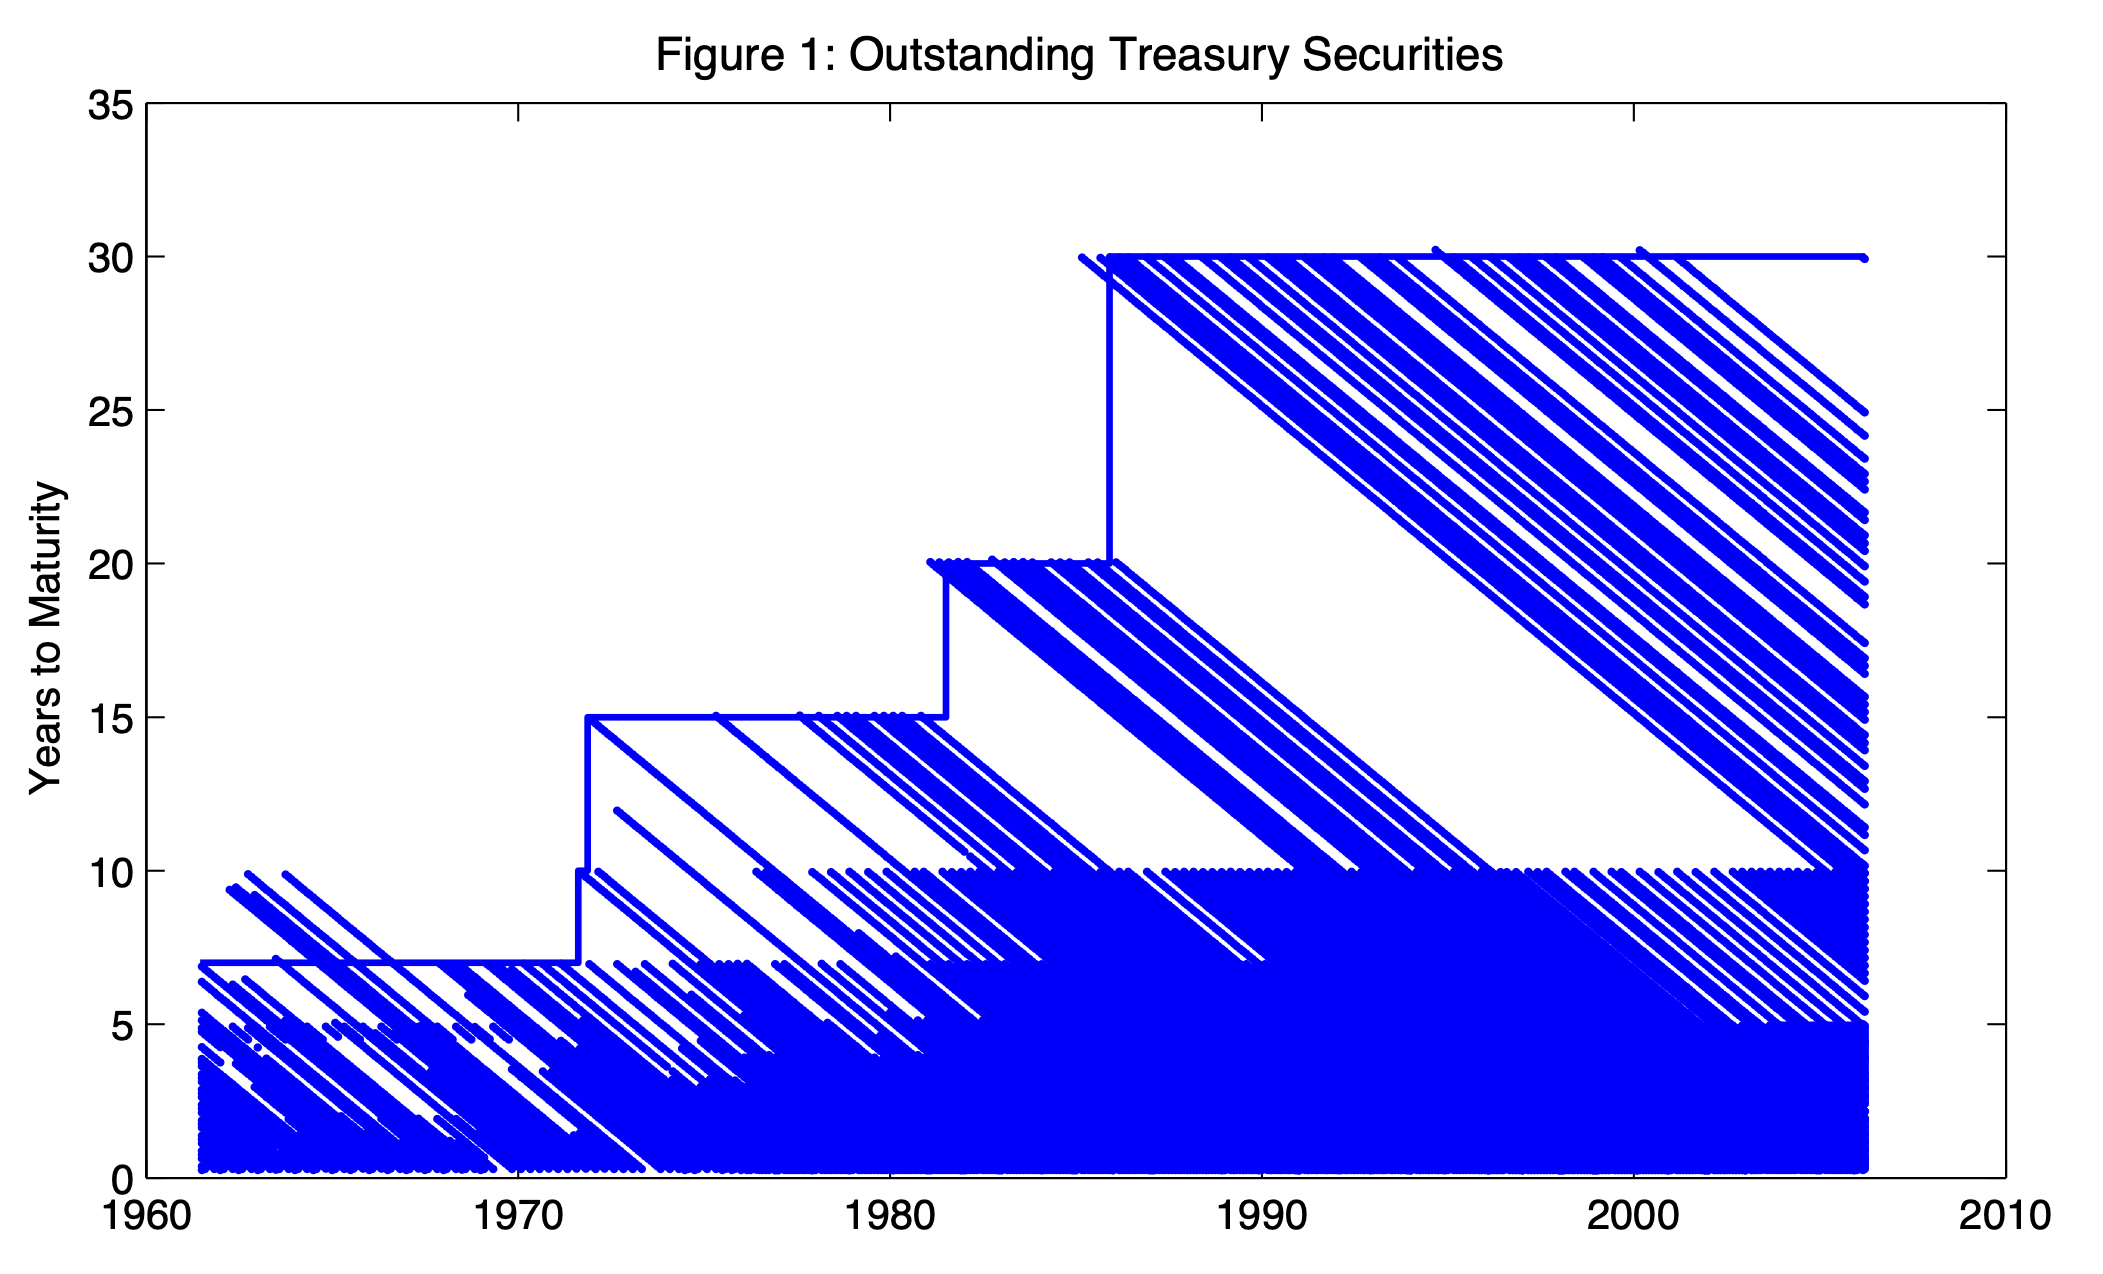
\includegraphics[width=0.9\linewidth]{figures/Fig_BdPortfolio} 

}

\caption{This figures displays the residual maturities of the bonds used for the estimation at the different dates of the sample. Source: Gurkaynak, Sack, and Wright (2007).}\label{fig:BdPortfolio}
\end{figure}

\begin{figure}

{\centering 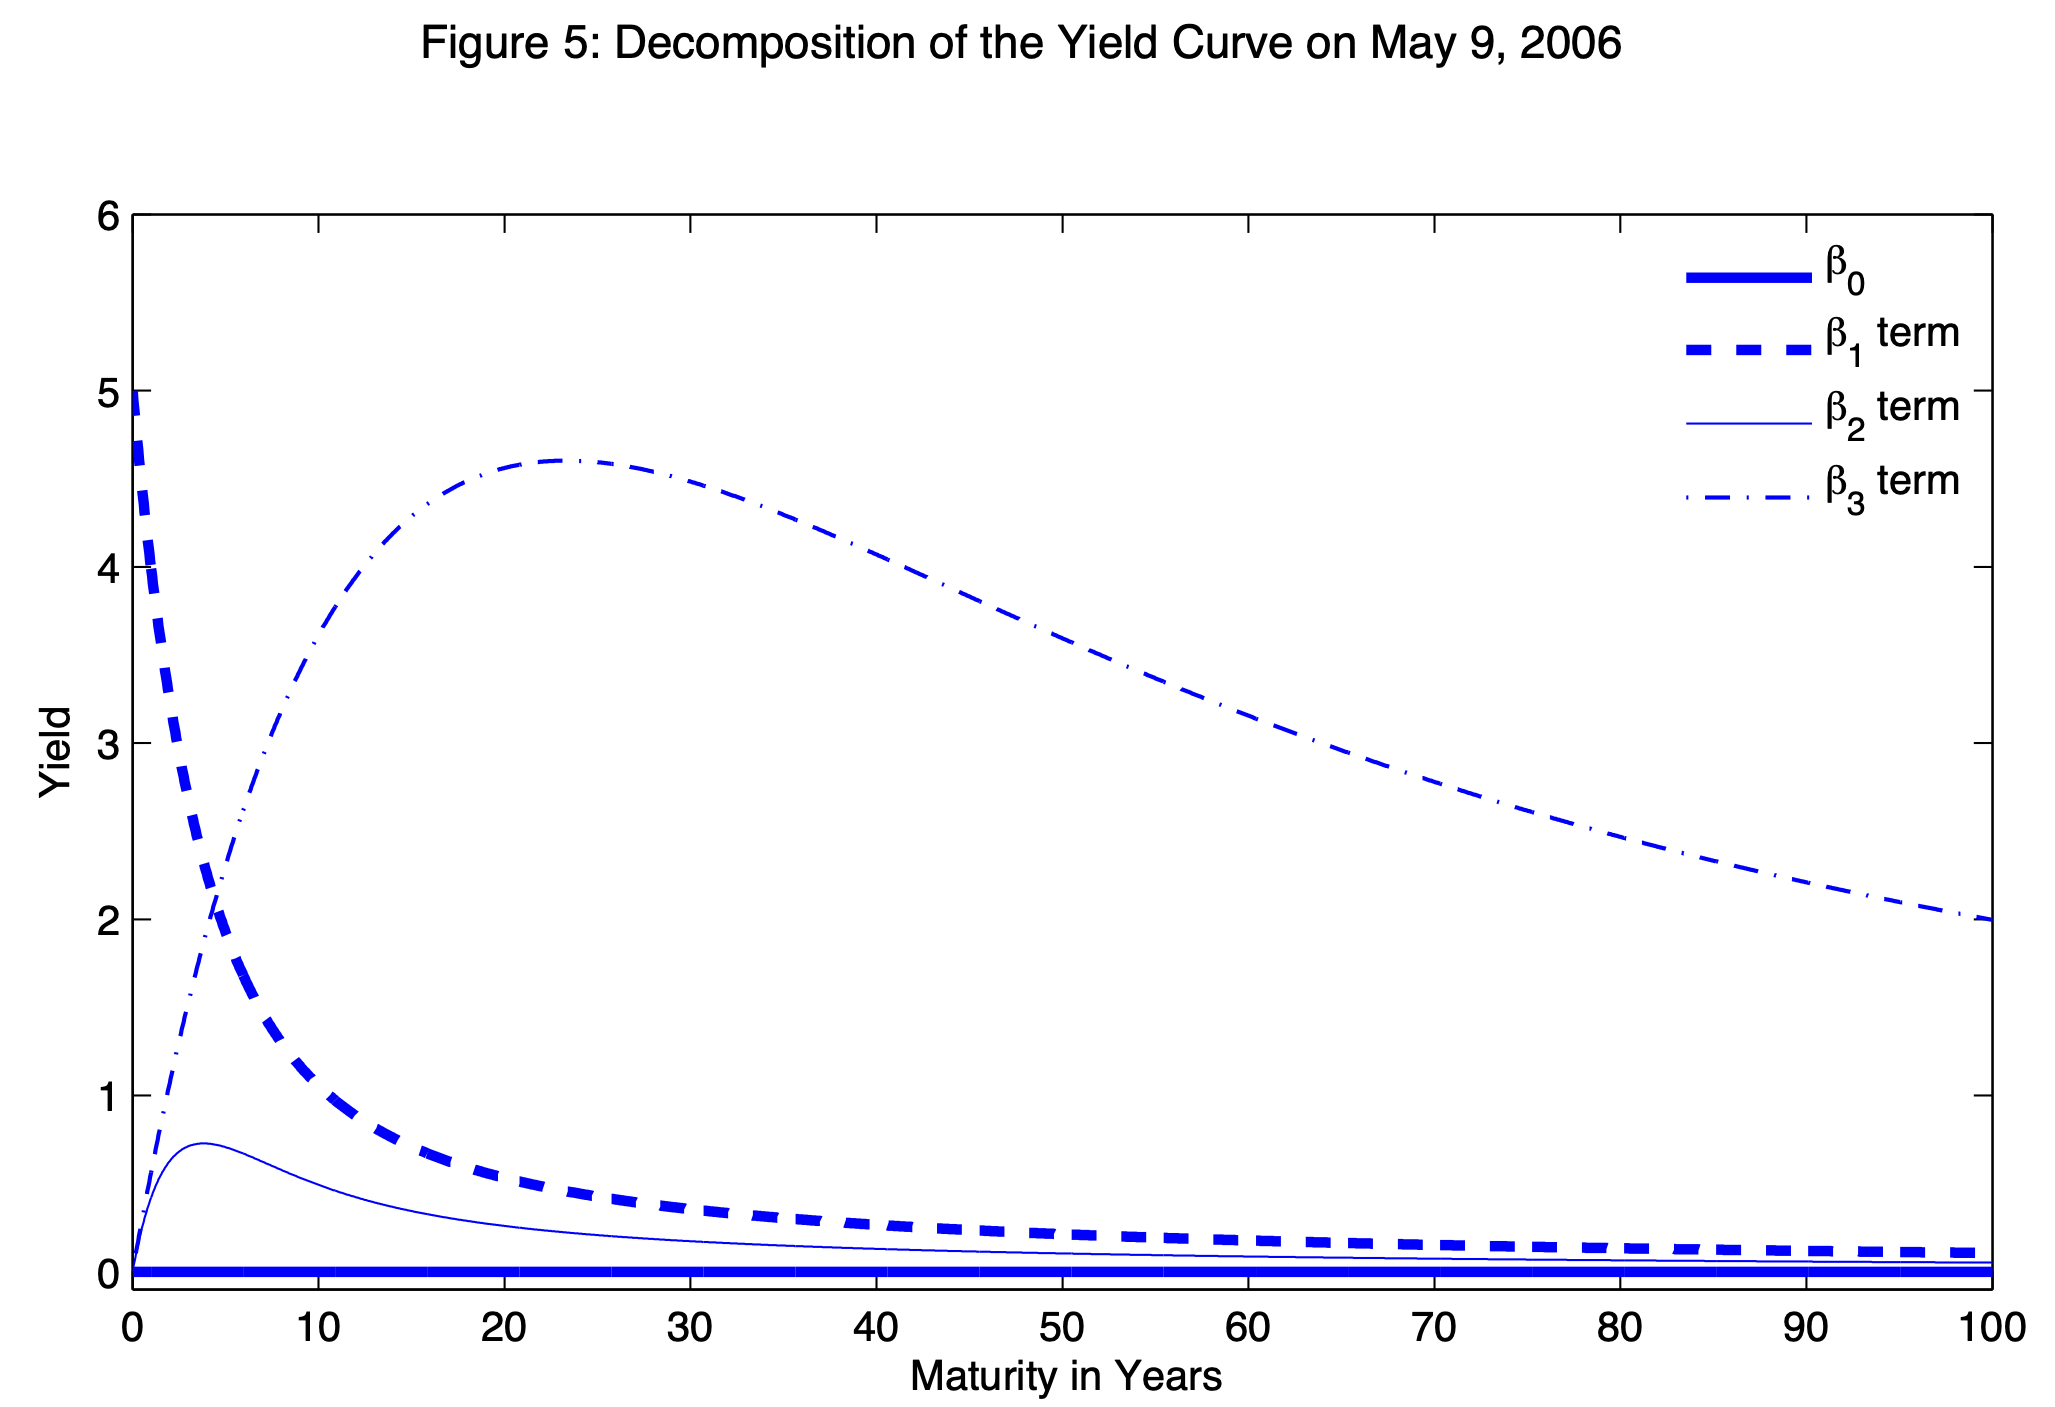
\includegraphics[width=0.9\linewidth]{figures/Fig_NSS} 

}

\caption{Example of yield curve decomposition using the Nelson-Siegel-Svensson parametric form. Source: Gurkaynak, Sack, and Wright (2007).}\label{fig:FigNSS}
\end{figure}

\begin{figure}

{\centering 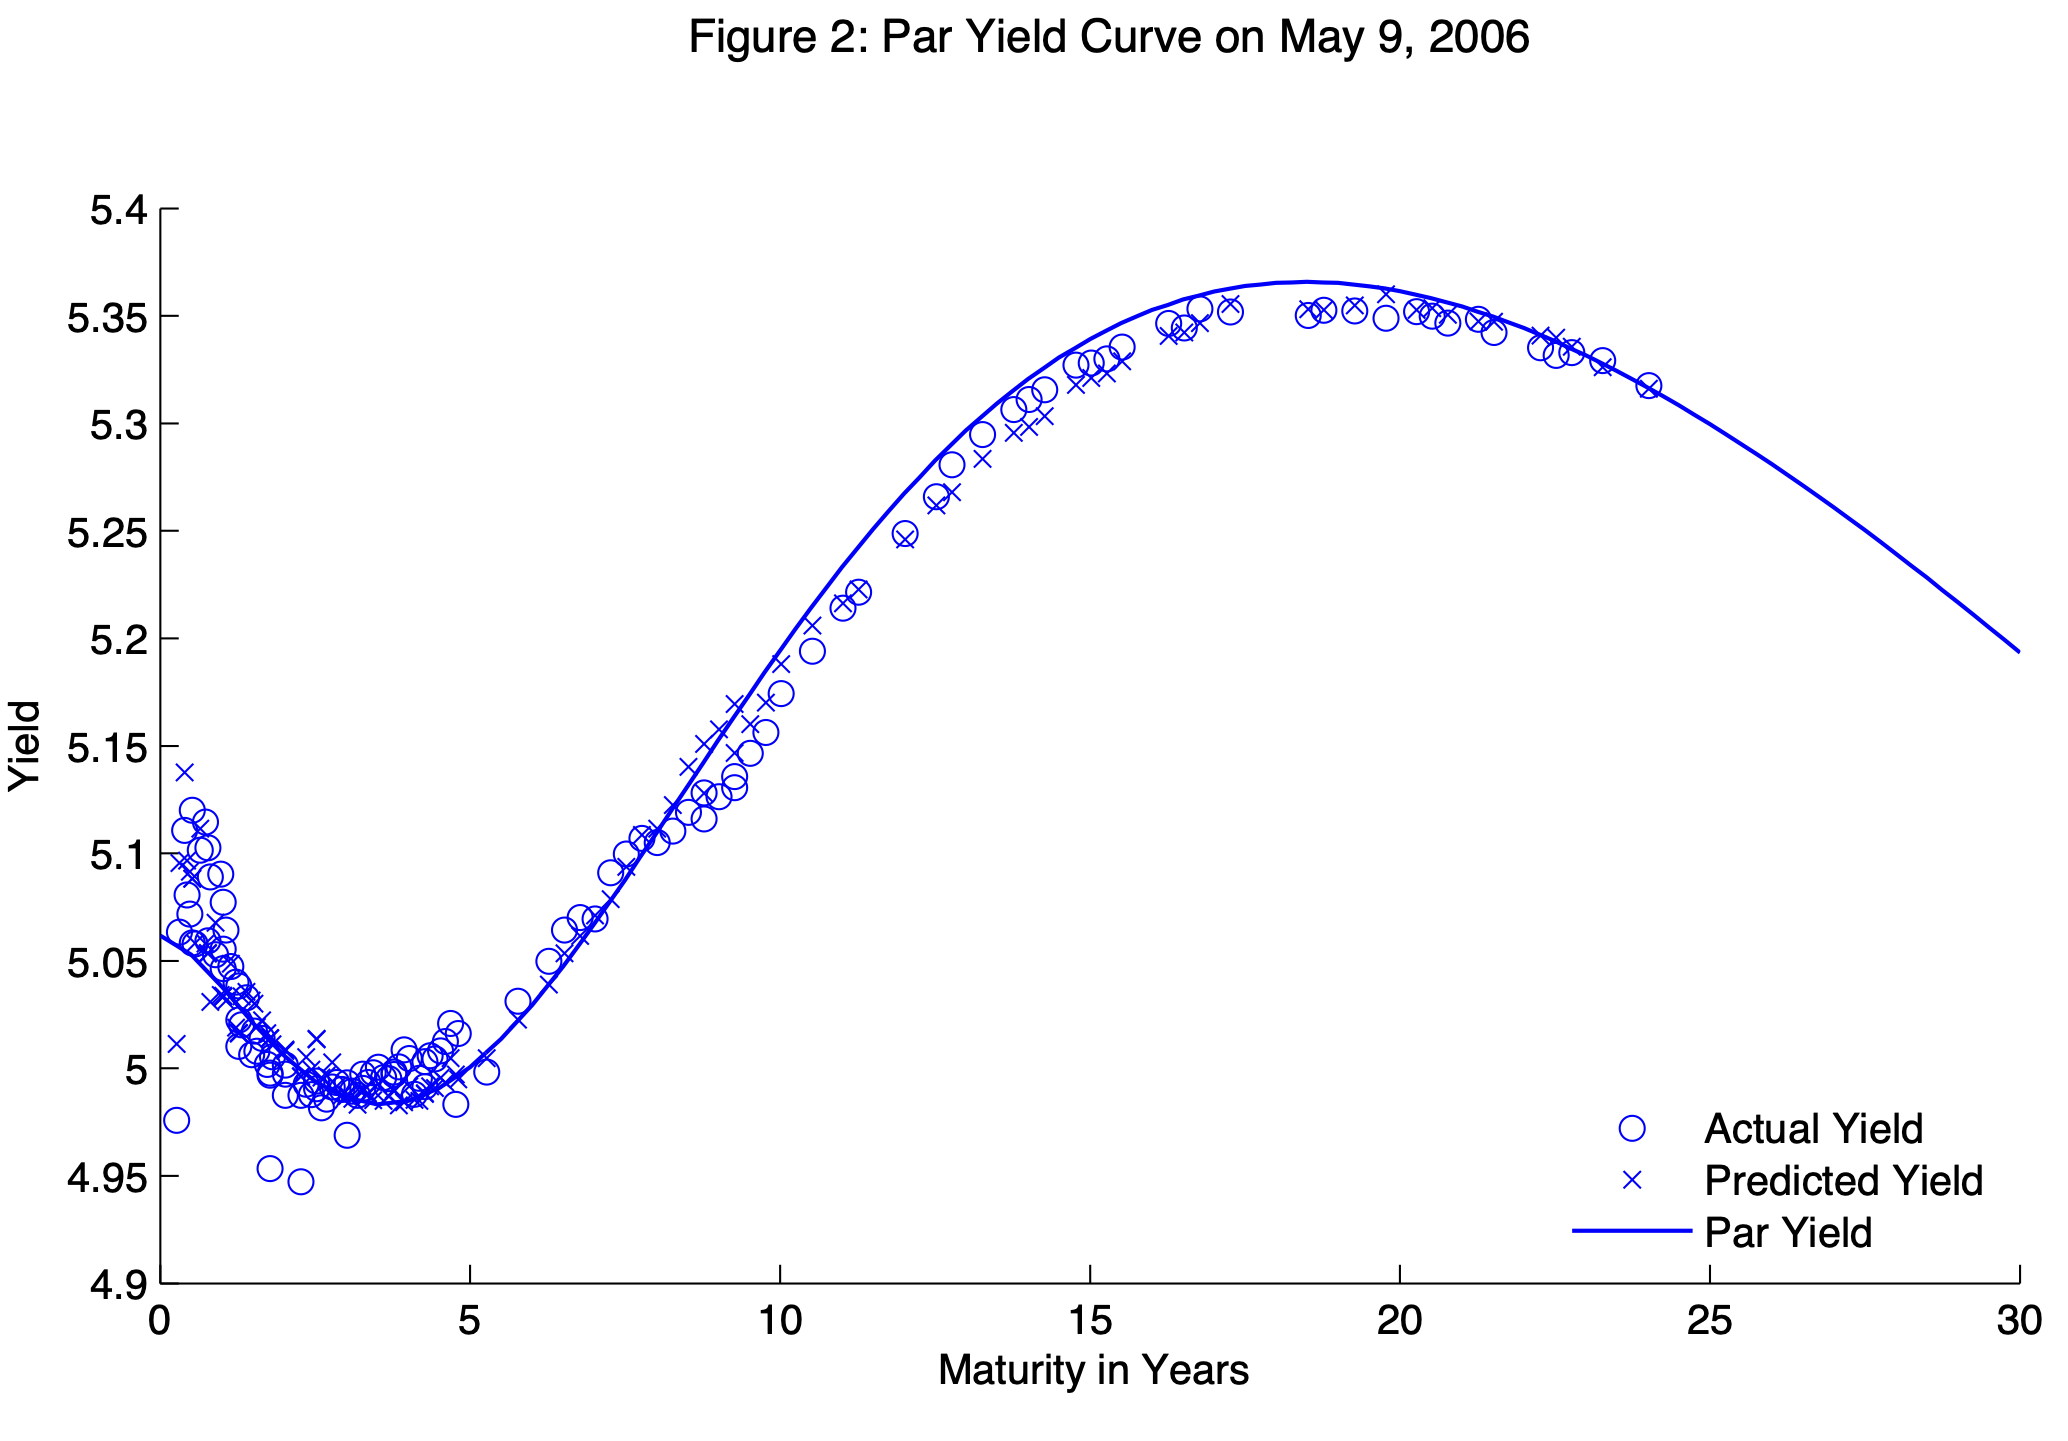
\includegraphics[width=0.9\linewidth]{figures/Fig_TSpar} 

}

\caption{This figure compares observed and fitted yields for a given date of the sample. Source: Gurkaynak, Sack, and Wright (2007).}\label{fig:Paryds}
\end{figure}

\end{example}

\hypertarget{swap-based-yield-curves}{%
\subsection{Swap-based yield curves}\label{swap-based-yield-curves}}

It is easy to obtain the maturity structure of swaps, since these instruments are ``constant maturity'' objects. In other words, every day, you can find a swap with a maturity of 1, 2,\ldots, 10 years (exactly). This contrasts with bonds, whose residual maturity is rarely a whole number of years.

Note however that swap yields are usually not zero-coupon yields. They are, instead, homogeneous to par yields, as defined in \eqref{eq:paryields} (see also the remark at the end of Subsection \ref{Swaps}). To obtain zero-coupon from the par yield curve, one can employ an approach called \emph{bootstrapping}. To simplify the exposition, we consider the yearly frequency. The bootstrapping approach operates recursively across maturities, using \eqref{eq:paryields}:

\begin{itemize}
\tightlist
\item
  Consider the one period maturity. We have:
  \[
  1 = \exp(-i_{t,1})(1 + i_{t,1}^p),
  \]
  which gives \(i_{t,1} = \log(1+i_{t,1}^p)\).
\item
  Next, for maturity 2, we have:
  \[
  1 = \exp(-2i_{t,2}) + \exp(-i_{t,1})i_{t,2}^p + \exp(-2i_{t,2})i_{t,2}^p,
  \]
  which gives \(i_{t,2} = \frac{1}{2}\log\left(1 + i_{t,2}^p \big/ 1 - \exp(-i_{t,1})i_{t,2}^p\right)\).
\item
  Using \eqref{eq:paryields} for \(h=3\) leads to a simple equation that can be solved to get \(i_{t,2}\) as a function of \(i_{t,3}^p\), \(i_{t,1}\), and \(i_{t,2}\).
\item
  idem for \(h=4\)\ldots{}
\end{itemize}

\hypertarget{Estimation}{%
\chapter{Estimation of affine asset-pricing models}\label{Estimation}}

\hypertarget{EstimationSSModel}{%
\section{State-space model}\label{EstimationSSModel}}

By nature, dynamic asset-pricing models are \emph{state-space models}: The dynamics of all variables of interest, gathered in vector \(y_t\) (yields, equity returns, macroeconomic variables, survey-based variables) are accounted for by state variables (\(w_t\)). The equations defining the relationship between the other variables and the state variables are called \emph{measurement equations} (Eq. \eqref{eq:measeq}). The equations defining the dynamics of the state variables are called \emph{transition equations} (Eq. \eqref{eq:transeq}).

In the case where \(w_t\) is an affine process (see Definition \ref{def:Car1}), the transition equations admit a VAR(1) representation (Proposition \ref{prp:affineVAR}). In that case, the state-space model is said to be linear, as formalized by the following definition. This defintion introduces, in particular, the notion of \emph{measurement errors}.

\begin{definition}[Linear State-Space Model]
\protect\hypertarget{def:LSSM}{}\label{def:LSSM}A linear state-space model writes as follows:
\begin{eqnarray}
\underset{(m \times 1)}{y_t}  &=& A + Bw_t + \eta_t  \quad \mbox{with }  \eta_t \sim i.i.d. \mathcal{N}(0,\Omega) \label{eq:measeq} \\
\underset{(n \times 1)}{w_t} & =& \mu + \Phi w_{t-1} + \Sigma^{\frac{1}{2}}(w_{t-1}) \varepsilon_t,\label{eq:transeq}
\end{eqnarray}
where \(\varepsilon_t\) is a martingale difference sequence satisfying \(\mathbb{V}ar_t(\varepsilon_{t+1}) = Id\). The components of \(\eta_t\) are measurement errors.
\end{definition}

\begin{quote}
\textbf{Note:} Eq. \eqref{eq:transeq} derives from Proposition \ref{prp:affineVAR} (Eq. \eqref{eq:VARw}).
\end{quote}

In practice, one can distinguish two situations: (a) all state variables (components of \(w_t\)) are observed and (b) some of these variables are latent. What do we mean by \emph{model estimation} in case (b)? One can distinguish different situations:

\begin{itemize}
\tightlist
\item
  (b.i) We know the model parameters but we want to recover the latent factors---for instance to compute model-implied prices.
\item
  (b.ii) We know neither the model parameters nor the latent variables, we want to estimate both of them.
\item
  (b.iii) We know neither the model parameters nor the latent variables, we are just interested in the model parameters.
\end{itemize}

In case (a): One can resort to standard estimation techniques (GMM, Maximum Likelihood) to estimate model parameters. Take for instance the maximum-likelihood case, we have:
\begin{eqnarray*}
f(y_t,w_t|\underline{y_{t-1}},\underline{w_{t-1}}) &=& f(y_t|\underline{y_{t-1}},\underline{w_{t}}) \times \underbrace{f(w_t|\underline{y_{t-1}},\underline{w_{t-1}})}_{= f(w_t|\underline{w_{t-1}})}\\
&=& \mathbf{n}(y_t;A + Bw_t,\Omega) f(w_t|\underline{w_{t-1}}),
\end{eqnarray*}
where \(\mathbf{n}(x;\mu,\Omega)\) denotes the evaluation, at vector \(x\), of the p.d.f. of the multivariate normal distribution \(\mathcal{N}(\mu,\Omega)\). That is, if \(x\) is a \(m\)-dimensional vector:
\begin{equation}
\mathbf{n}(x;\mu,\Omega) = \frac{1}{\sqrt{(2 \pi)^{m}|\Omega|}} \exp\left(-\frac{1}{2}\{x - \mu\}'\Omega^{-1}\{x-\mu\}\right).\label{eq:varPHI}
\end{equation}
Once this conditional p.d.f. is known, the total likelihood is given by (conditional on \(y_0\) and \(w_0\)):
\[
\prod_{t=1}^T f(y_t,w_t|\underline{y_{t-1}},\underline{w_{t-1}}).
\]
Of course, \(f(w_t|\underline{w_{t-1}})\) depends on the process chosen for \(w_t\). If it is complicated to compute, one can employ Pseudo Maximum Likelihood (PML) \citep{Gourieroux_Monfort_Trognon_1984}. The p.d.f. may involve, for instance, an infinite sum, which is the case in the ARG case of Example \ref{exm:ARG1}. When \(w_t\) is affine, the Pseudo Maximum Likelihood approach consists in replacing \(f(w_t|\underline{w_{t-1}})\) by:
\[
\mathbf{n}(w_t;\mu + \Phi w_{t-1},\Sigma(w_t)),
\]
where \(\mu\), \(\Phi\) and \(\Sigma(w_t)\) are defined in \eqref{eq:MUPHI} and \eqref{eq:SigmaWt} in Proposition \ref{prp:affineVAR}.

In case (b.iii), one can estimate the model by Generalized Method of Moments (GMM), fitting sample moments computed using observed variables (prices, yields, returns). In the context of affine processes, conditional and unconditional moments of the state vector \(w_t\) are available in closed from, as shown by \eqref{eq:condmean}, \eqref{eq:condvar} and \eqref{eq:uncondmeanvar}. If the model-implied moments are not available in closed-form, one may have to to resort to the \emph{Simulated Method of Moments (SMM)} (see, e.g., \citet{GourMonf96} or \citet{Duffie_Singleton_1993}).

In cases (b.i) and (b.ii), one has to implement \emph{filtering methods}, on which we focus on in the following.

\hypertarget{Estimation:KF}{%
\section{Kalman-filter-based approach}\label{Estimation:KF}}

\hypertarget{the-gaussian-linear-state-space-case}{%
\subsection{The Gaussian linear state-space case}\label{the-gaussian-linear-state-space-case}}

Let us start with a particular case of state-space model (Def. \ref{def:LSSM}) where \(\varepsilon_t\) is Gaussian and where \(\Sigma^{\frac{1}{2}}\) does not depend on \(w_t\), i.e., with a homoskedastic linear Gaussian state-space model.

Denote by \(\theta\) the vector of parameters that defines the model. For a given \(\theta\) and a sequence of observations \(\{y_1,\dots,y_T\}\), the Kalman filter computes the distribution of \(w_t\) given \(\{y_1,\dots,y_t\}\) (see Def. \ref{def:FiltvsSmooth}). This distribution is Gaussian, and obtained by a recursive algorithm. A byproduct of this algorithm is the likelihood function associated with \(\theta\) and \(\{y_1,\dots,y_T\}\). This opens the door to the estimation of \(\theta\) by MLE, maximizing this function. In this sense, Kalman-filter techniques can address Objective (b.ii).

Let us first introduce the notion of \emph{filtered} and \emph{smoothed} estimates of a latent variable (or vector of variables) \(w_t\):

\begin{definition}[Filtered versus smoothed estimates]
\protect\hypertarget{def:FiltvsSmooth}{}\label{def:FiltvsSmooth}The filtering and smoothing problems consist in computing the following conditional moments:
\begin{equation*}
\begin{array}{lccllllll}
\mbox{Filtering:} & w_{t|t} & = & \mathbb{E}(w_t|\underline{y_t}) & \mbox{and}  & P_{t|t} &=& \mathbb{V}ar(w_t|\underline{y_t})\\
\mbox{Smoothing:} & w_{t|T} & = & \mathbb{E}(w_t|\underline{y_T}) & \mbox{and} & P_{t|T} &=& \mathbb{V}ar(w_t|\underline{y_T}).
\end{array}
\end{equation*}
\end{definition}

The following proposition outlines the Kalman algorithm (see, e.g. \citet{Kim_Nelson_1999}).

\begin{proposition}[Kalman filter and smoother]
\protect\hypertarget{prp:KF}{}\label{prp:KF}If \(\varepsilon_t \sim \mathcal{N}(0,I)\) in the state-space defined in Def. \ref{def:LSSM}, then we have (\emph{filtering}):
\[
w_t|y_1,\dots,y_t \sim  \mathcal{N}(w_{t|t}|P_{t|t}),
\]
where \(w_{t|t}\) and \(P_{t|t}\) result from the following recursive equations:
\[
\boxed{
\begin{array}{ccl}
w_{t|t} &=& w_{t|t-1} + K_t \lambda_t\\
P_{t|t} &=& (I - K_t B)P_{t|t-1} \\ \\
\mbox{where (updating step)} \\
\lambda_t &=& y_t - A - Bw_{t|t-1}  \quad \mbox{(forecast error)}\\
S_{t|t-1} &=& \mathbb{V}ar(y_t|\underline{y_{t-1}}) = B P_{t|t-1} B' + \Omega\\
K_t &=& P_{t|t-1}B'S_{t|t-1}^{-1} \quad \mbox{(Kalman gain)} \\ \\
\mbox{and where (forecasting step)} \\
w_{t|t-1} &=& \mu + \Phi w_{t-1|t-1} \\
P_{t|t-1} &=& \Sigma + \Phi P_{t-1|t-1} \Phi' \quad (\Sigma = \Sigma^{\frac{1}{2}}{\Sigma^{\frac{1}{2}}}').
\end{array}
}
\]
The log likelihood is (recursively) computed as follows:
\begin{eqnarray}
\log \mathcal{L}(\theta;\underline{y_T}) &=& \frac{mT}{2}\log\left(2\pi\right) \label{eq:logLikKF}\\
&  & -\frac{1}{2}\sum_{t=1}^{T}\left(\log\left|S_{t | t-1}(\theta)\right|+\lambda'_{t}(\theta)S_{t\mid t-1}^{-1}(\theta)\lambda{}_{t}(\theta)\right). \nonumber
\end{eqnarray}

Moreover, we have (\emph{smoothing}):
\[
w_t|y_1,\dots,y_T \sim  \mathcal{N}(w_{t|T}|P_{t|T}),
\]
where \(w_{t|T}\) and \(P_{t|T}\) result from the following recursive equations:
\[
\boxed{
\begin{array}{ccl}
w_{t|T} & = & w_{t|t}+F_{t}(w_{t+1|T}-w_{t+1|t})\\
P_{t|T} & = & P_{t|t}+F_{t}(P_{t+1|T}-P_{t+1|t})F'_{t}\\ \\
\mbox{where} \\
F_{t} &=& P_{t|t}\Phi'_{t+1}P_{t+1|t}^{-1}.
\end{array}
}
\]
\end{proposition}

The following figure illustrates the updating step of the Kalman algorithm:

\begin{figure}
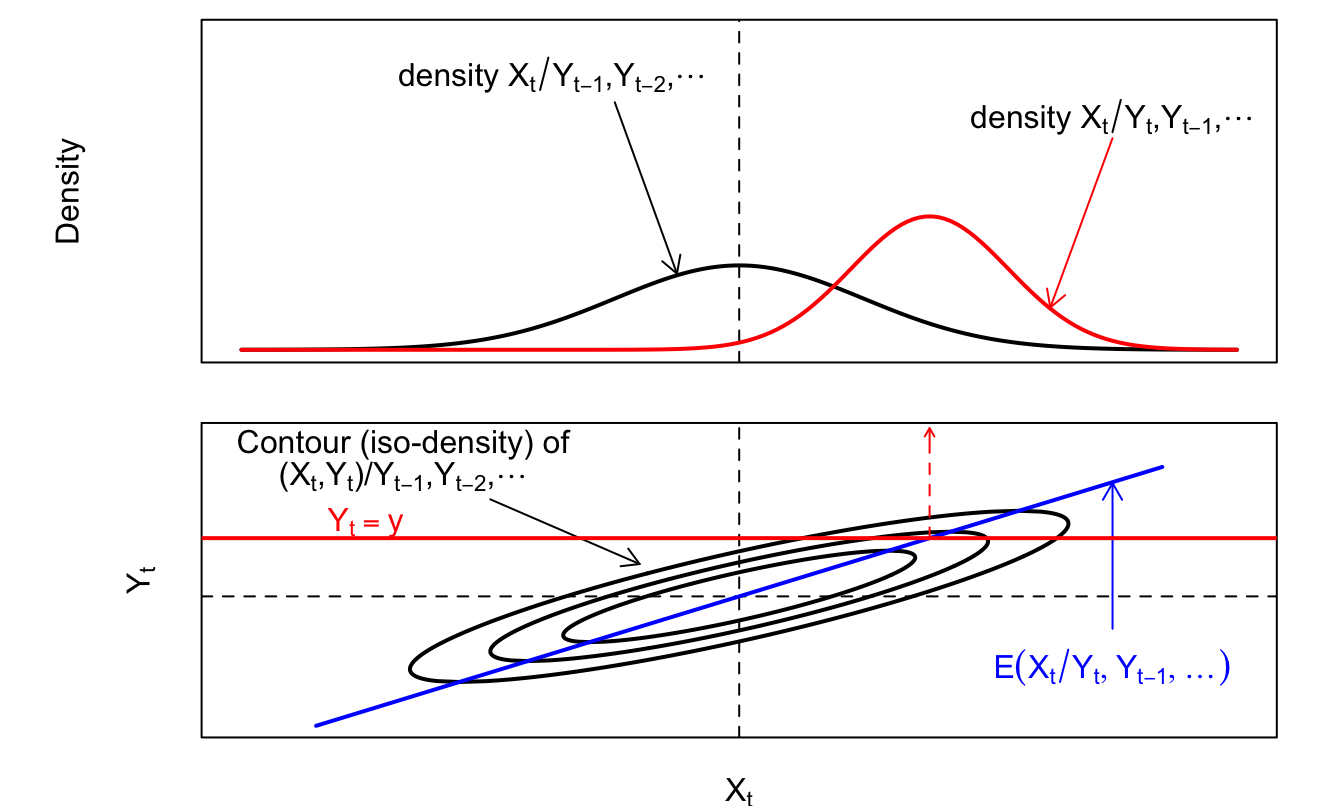
\includegraphics[width=0.95\linewidth]{TSM_files/figure-latex/illusKF-1} \caption{Updating in the Kalman filter.}\label{fig:illusKF}
\end{figure}

The recursive equations of the Kalman filter need to be initialized. That is, one needs to provide initial values for \(w_{0|0}\), \(P_{0|0}\). Different possibilities have been proposed. One can for instance:

\begin{itemize}
\tightlist
\item
  Include the elements of(\(w_{0|0}\), \(P_{0|0}\)) among the parameters to estimate;
\item
  Set \(w_{0|0}\) and \(P_{0|0}\) to their unconditional values (using, e.g., \eqref{eq:uncondmeanvar});
\item
  Set \(w_{0|0}\) to a prior value and take either an arbitrary large value for \(P_{0\mid0}\) if the prior value is uncertain (which depicts a situation of \emph{diffuse prior}) or a small value for \(P_{0\mid0}\) if we are confident in this prior value \(w_{0|0}\).
\end{itemize}

\begin{example}[Kalman filtering and smoothing]
\protect\hypertarget{exm:RKalman}{}\label{exm:RKalman}

To illustrate, consider the following model:
\begin{eqnarray}
\left[\begin{array}{c}
y_{1,t}\\
y_{2,t}
\end{array}\right] & = &
\left[\begin{array}{cc}
\alpha_{1} & 0\\
0 & \alpha_{2}
\end{array}\right]
\left[\begin{array}{c}
y_{1,t-1}\\
y_{2,t-2}
\end{array}\right]+\left[\begin{array}{c}
\gamma_{1}\\
\gamma_{2}
\end{array}\right]w_{t}+ D\eta_t\label{eq_measur}\\
w_{t} & = & \phi w_{t-1}+\varepsilon_{t},\label{eq_trans}
\end{eqnarray}
where \(\eta_t \sim \mathcal{N}(0,Id)\).

In the following lines, we specify one version of the previous model. We simulate trajectories of \(y_{1,t}\), \(y_{2,t}\) and \(w_t\) over 100 periods (Figure \ref{fig:Kalmansimul}) and we further call \texttt{Kalman\_filter} and \texttt{Kalman\_filter} (from the \texttt{TSModels} package) to compute the filtered and smoothed estimates of \(w_t\) (Figure \ref{fig:Kalman2}).

\begin{Shaded}
\begin{Highlighting}[]
\FunctionTok{library}\NormalTok{(TSModels) }\CommentTok{\# Kalman filter procedure in there.}
\CommentTok{\# Set model specifications:}
\NormalTok{alpha1 }\OtherTok{\textless{}{-}}\NormalTok{ .}\DecValTok{5}\NormalTok{;alpha2 }\OtherTok{\textless{}{-}}\NormalTok{ .}\DecValTok{95}\NormalTok{;Alpha }\OtherTok{\textless{}{-}} \FunctionTok{diag}\NormalTok{(}\FunctionTok{c}\NormalTok{(alpha1,alpha2))}
\NormalTok{d\_11 }\OtherTok{\textless{}{-}} \DecValTok{1}\NormalTok{;d\_12 }\OtherTok{\textless{}{-}}\NormalTok{ .}\DecValTok{5}\NormalTok{;d\_21 }\OtherTok{\textless{}{-}}\NormalTok{ .}\DecValTok{5}\NormalTok{;d\_22 }\OtherTok{\textless{}{-}} \DecValTok{2}
\NormalTok{D }\OtherTok{\textless{}{-}} \FunctionTok{matrix}\NormalTok{(}\FunctionTok{c}\NormalTok{(d\_11,d\_21,d\_12,d\_22),}\DecValTok{2}\NormalTok{,}\DecValTok{2}\NormalTok{)}
\NormalTok{gamma1 }\OtherTok{\textless{}{-}} \DecValTok{1}\NormalTok{;gamma2 }\OtherTok{\textless{}{-}} \DecValTok{2}\NormalTok{;Gamma }\OtherTok{\textless{}{-}} \FunctionTok{matrix}\NormalTok{(}\FunctionTok{c}\NormalTok{(gamma1,gamma2),}\DecValTok{2}\NormalTok{,}\DecValTok{1}\NormalTok{)}
\NormalTok{phi }\OtherTok{\textless{}{-}}\NormalTok{ .}\DecValTok{8}
\CommentTok{\# Simulate model:}
\NormalTok{T }\OtherTok{\textless{}{-}} \DecValTok{100}
\NormalTok{Y }\OtherTok{\textless{}{-}} \ConstantTok{NULL}\NormalTok{;X }\OtherTok{\textless{}{-}} \ConstantTok{NULL}
\NormalTok{Alpha.Y\_1 }\OtherTok{\textless{}{-}} \ConstantTok{NULL}
\NormalTok{y }\OtherTok{\textless{}{-}} \FunctionTok{c}\NormalTok{(}\DecValTok{0}\NormalTok{,}\DecValTok{0}\NormalTok{);x }\OtherTok{\textless{}{-}} \DecValTok{0}
\ControlFlowTok{for}\NormalTok{(i }\ControlFlowTok{in} \DecValTok{1}\SpecialCharTok{:}\NormalTok{T)\{}
\NormalTok{  Alpha.Y\_1 }\OtherTok{\textless{}{-}} \FunctionTok{rbind}\NormalTok{(Alpha.Y\_1,}\FunctionTok{c}\NormalTok{(Alpha }\SpecialCharTok{\%*\%}\NormalTok{ y))}
\NormalTok{  y }\OtherTok{\textless{}{-}}\NormalTok{ Alpha }\SpecialCharTok{\%*\%}\NormalTok{ y }\SpecialCharTok{+}\NormalTok{ Gamma }\SpecialCharTok{*}\NormalTok{ x }\SpecialCharTok{+}\NormalTok{ D }\SpecialCharTok{\%*\%} \FunctionTok{rnorm}\NormalTok{(}\DecValTok{2}\NormalTok{)}
\NormalTok{  x }\OtherTok{\textless{}{-}}\NormalTok{ phi }\SpecialCharTok{*}\NormalTok{ x }\SpecialCharTok{+} \FunctionTok{rnorm}\NormalTok{(}\DecValTok{1}\NormalTok{)}
\NormalTok{  Y }\OtherTok{\textless{}{-}} \FunctionTok{rbind}\NormalTok{(Y,}\FunctionTok{t}\NormalTok{(y));X }\OtherTok{\textless{}{-}} \FunctionTok{rbind}\NormalTok{(X,x)\}}
\CommentTok{\# Define matrices needed in the Kalman\_filter procedures:}
\NormalTok{nu\_t }\OtherTok{\textless{}{-}} \FunctionTok{matrix}\NormalTok{(}\DecValTok{0}\NormalTok{,T,}\DecValTok{1}\NormalTok{)}
\NormalTok{H }\OtherTok{\textless{}{-}}\NormalTok{ phi;G }\OtherTok{\textless{}{-}}\NormalTok{ Gamma}
\NormalTok{mu\_t }\OtherTok{\textless{}{-}}\NormalTok{ Alpha.Y\_1}
\NormalTok{N }\OtherTok{\textless{}{-}} \DecValTok{1}\NormalTok{;M }\OtherTok{\textless{}{-}}\NormalTok{ D}
\NormalTok{Sigma\_0 }\OtherTok{\textless{}{-}} \DecValTok{1}\SpecialCharTok{/}\NormalTok{(}\DecValTok{1}\SpecialCharTok{{-}}\NormalTok{phi}\SpecialCharTok{\^{}}\DecValTok{2}\NormalTok{) }\CommentTok{\# unconditional variance of w}
\NormalTok{rho\_0 }\OtherTok{\textless{}{-}} \DecValTok{0} \CommentTok{\# unconditional mean of w}
\NormalTok{filter.res   }\OtherTok{\textless{}{-}} \FunctionTok{Kalman\_filter}\NormalTok{(Y,nu\_t,H,N,mu\_t,G,M,Sigma\_0,rho\_0)}
\NormalTok{smoother.res }\OtherTok{\textless{}{-}} \FunctionTok{Kalman\_smoother}\NormalTok{(Y,nu\_t,H,N,mu\_t,G,M,Sigma\_0,rho\_0)}
\end{Highlighting}
\end{Shaded}

\begin{figure}
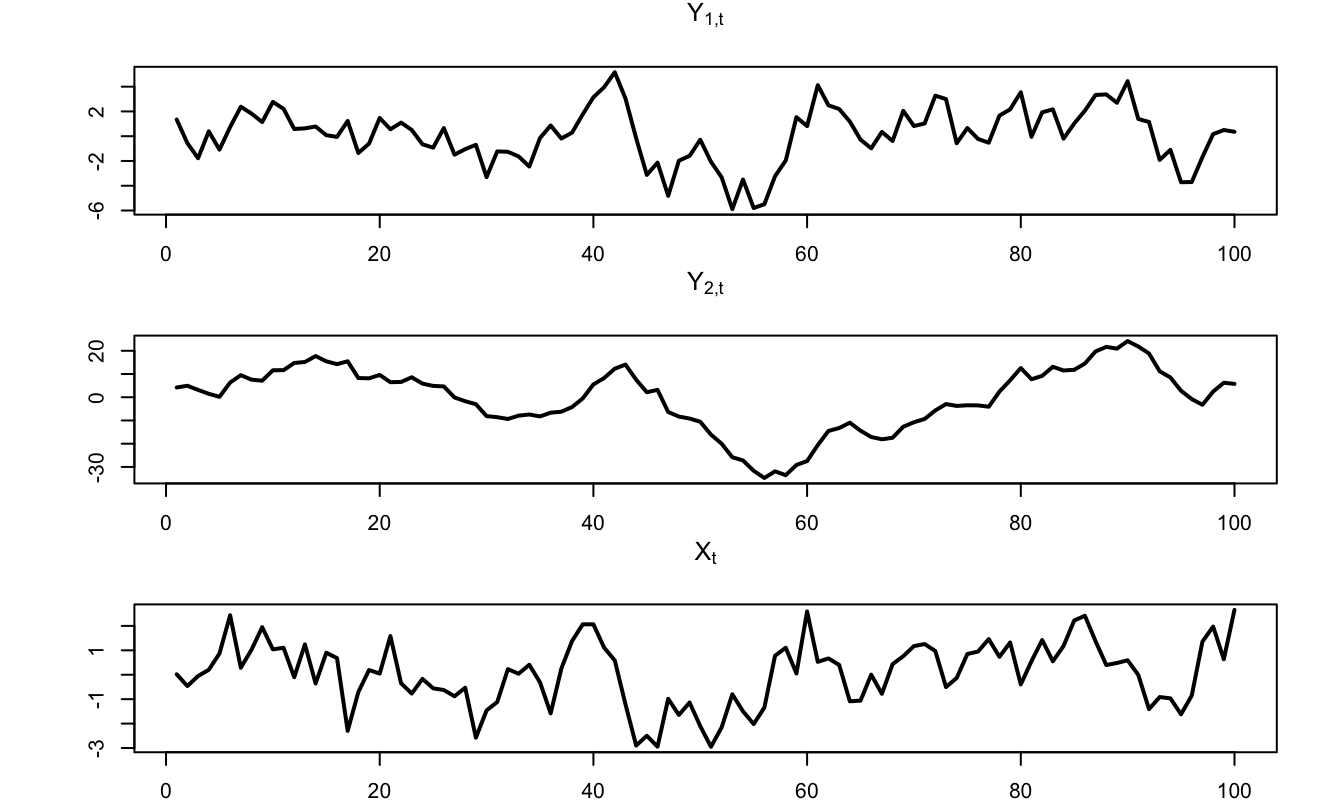
\includegraphics[width=0.95\linewidth]{TSM_files/figure-latex/Kalmansimul-1} \caption{Simulated trajectories of $y_{1,t}$, $y_{2,t}$, and $w_t$.}\label{fig:Kalmansimul}
\end{figure}

\begin{figure}
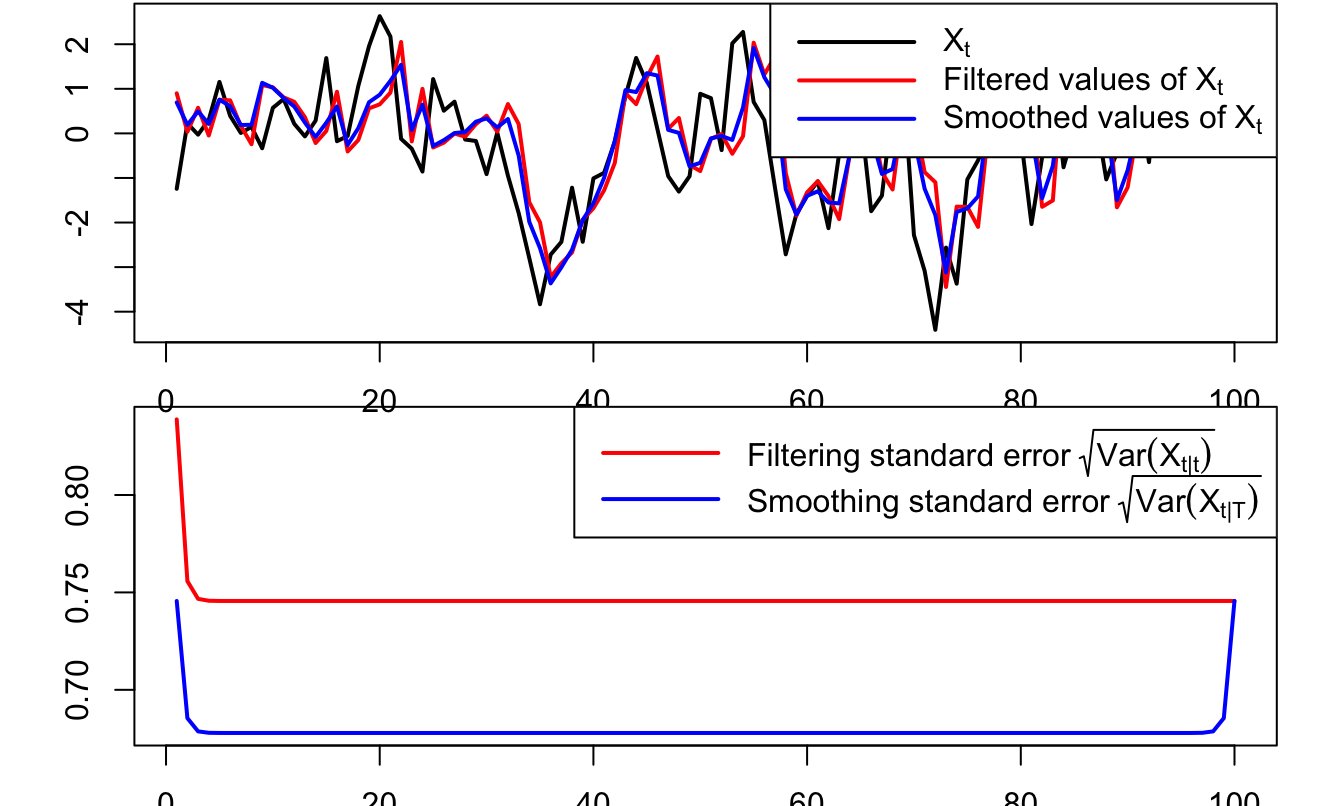
\includegraphics[width=0.95\linewidth]{TSM_files/figure-latex/Kalman2-1} \caption{Filtered and smoothed estimates of $w_t$.}\label{fig:Kalman2}
\end{figure}

\end{example}

\hypertarget{missing-observations}{%
\subsection{Missing observations}\label{missing-observations}}

In many application, one does not observe all the entries of \(y_t\) at every date. This arises for instance in situations where (i) measurement variables feature different frequencies, (ii) we have unreliable data for some period (that we prefer not to include among observations), (iii) some of the measurement variables are observed over a shorter time span.

These situations are easily addressed by Kalman filtering/smoothing (e.g., \citet{Chow_Lin_1971} or \citet{Harvey_Pierse_1984}). To accommodate missing observations in some of the \(y_t\)'s, one simply has to change the size of this vector (and of \(\lambda_t\), \(S_{t|t-1}\), \(A\) and \(B\)) for the relevant dates. Of course, the accuracy of \(w_{t|t}\) will tend to be lower during periods where one or several (or all) the entries of \(y_t\) are unobserved. (This will be apparent in the resulting covariance matrix of \(w_{t|t}\), namely \(P_{t|t}\).) The log-likelihood computation of \eqref{eq:logLikKF} is still valid in this case; one simply has to adjust the number of observed variables at each iteration; that is, \(m\) then depends on time.

\begin{example}[Kalman filtering and smoothing]
\protect\hypertarget{exm:RKalmanMissing}{}\label{exm:RKalmanMissing}

This example extends Example \ref{exm:RKalmanMissing}. We take the simulated path of the obeerved variables \(y_{1,t}\) and \(y_{2,t}\) and remove observations of \(y_{1,t}\) (respectively of \(y_{2,t}\)) between periods \(t=30\) and \(t=50\) (resp. between periods \(t=40\) and \(t=70\)), and then use the Kalman filter and smother to recover the states \(w_t\) in this situation with missing observations.

\begin{Shaded}
\begin{Highlighting}[]
\NormalTok{Y.modif }\OtherTok{\textless{}{-}}\NormalTok{ Y}
\NormalTok{Y.modif[}\DecValTok{30}\SpecialCharTok{:}\DecValTok{50}\NormalTok{,}\DecValTok{1}\NormalTok{] }\OtherTok{\textless{}{-}} \ConstantTok{NaN}
\NormalTok{Y.modif[}\DecValTok{40}\SpecialCharTok{:}\DecValTok{70}\NormalTok{,}\DecValTok{2}\NormalTok{] }\OtherTok{\textless{}{-}} \ConstantTok{NaN}
\CommentTok{\# Call of Kalman filter and smoother:}
\NormalTok{filter.res   }\OtherTok{\textless{}{-}} \FunctionTok{Kalman\_filter}\NormalTok{(Y.modif,nu\_t,H,N,mu\_t,}
\NormalTok{                              G,M,Sigma\_0,rho\_0)}
\NormalTok{smoother.res }\OtherTok{\textless{}{-}} \FunctionTok{Kalman\_smoother}\NormalTok{(Y.modif,nu\_t,H,N,mu\_t,}
\NormalTok{                                G,M,Sigma\_0,rho\_0)}
\end{Highlighting}
\end{Shaded}

\begin{figure}
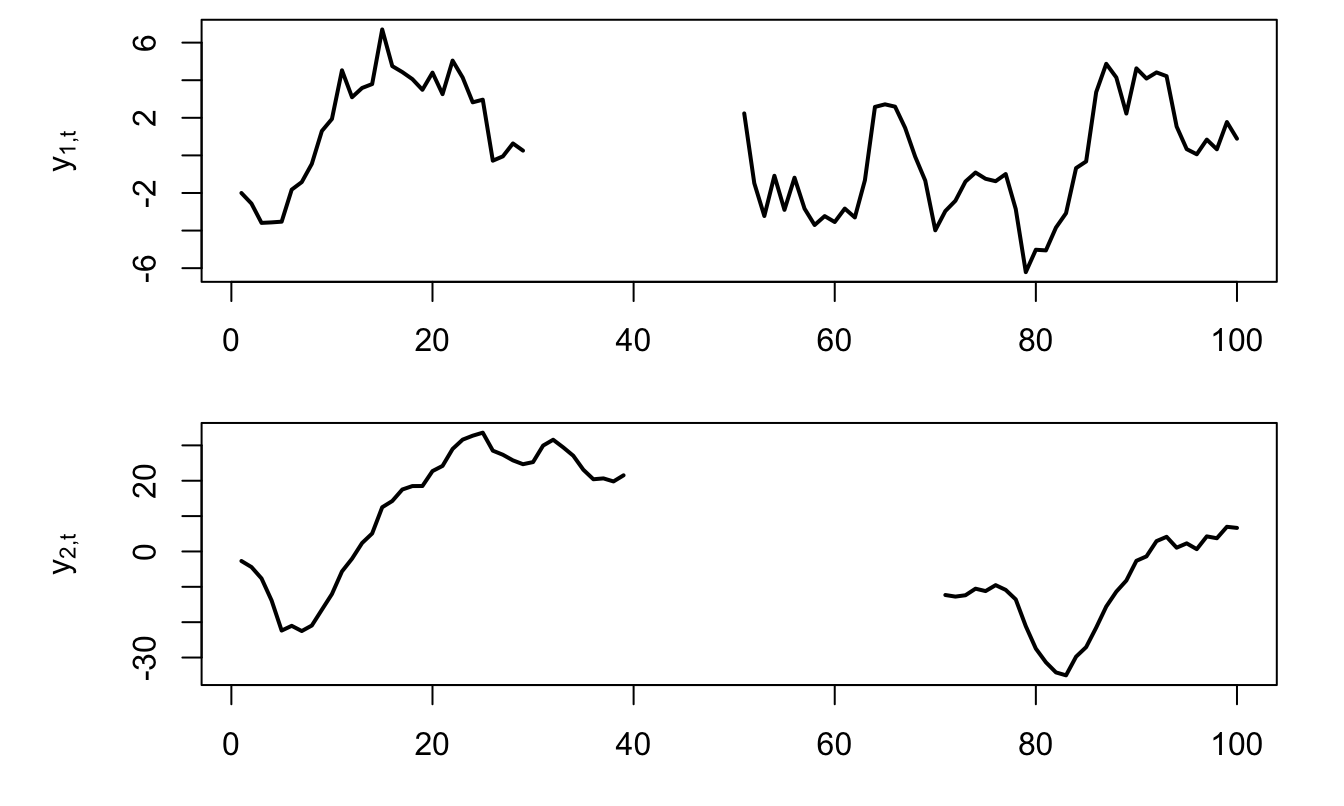
\includegraphics[width=0.95\linewidth]{TSM_files/figure-latex/Kalman5-1} \caption{Situation of missing observations.}\label{fig:Kalman5}
\end{figure}

\begin{figure}
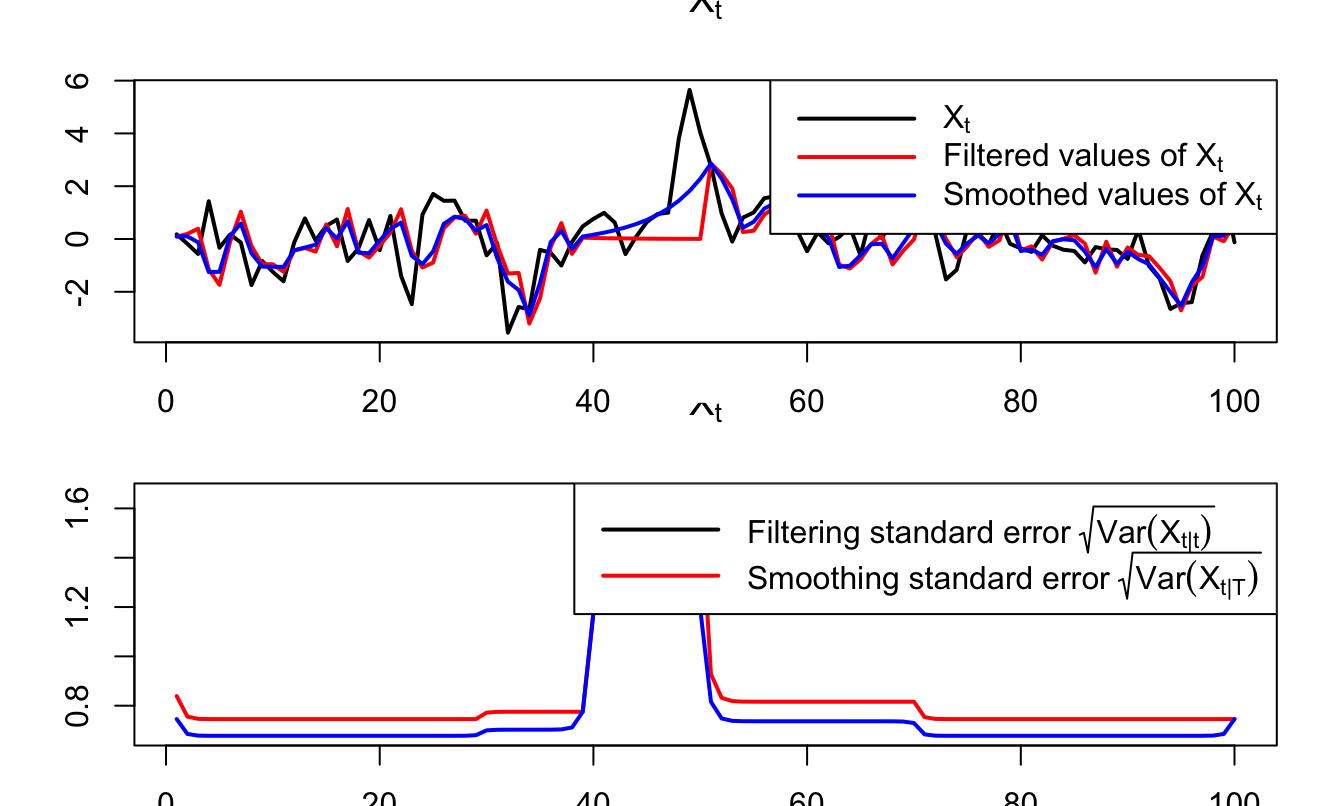
\includegraphics[width=0.95\linewidth]{TSM_files/figure-latex/Kalman6-1} \caption{Filtered and smoothed estimates of $w_t$ in a situation of missing observations. The lower plot shows the standard errors associated with filtered and smoothed estimates. As expected, undertainty is larger for those dates where observations are missing.}\label{fig:Kalman6}
\end{figure}

\end{example}

\hypertarget{KalmanQML}{%
\subsection{\texorpdfstring{About non-constant conditional matrix \(\Sigma\)}{About non-constant conditional matrix \textbackslash Sigma}}\label{KalmanQML}}

Proposition \ref{prp:KF} is valid when \(\varepsilon_t\) is Gaussian and when \(\Sigma^{\frac{1}{2}}\) does not depend on \(w_t\). However, in the general case (but when \(w_t\) is an affine process), we have that \(\Sigma(w_{t-1}) \equiv \mathbb{V}ar(w_{t+1}|\underline{w_t})\) is affine in \(w_t\) (see Prop. \ref{prp:affineVAR}). In order to deal with this, the Kalman filter algorithm can be modified. Specifically, in the prediction step (see Prop. \ref{prp:KF}), \(P_{t|t-1}\) can be approximated by:
\[
P_{t|t-1} = \Sigma\color{red}{(w_{t-1|t-1})} + \Phi P_{t-1|t-1} \Phi',
\]
i.e., we replace \(\Sigma(w_{t-1})\) by \(\Sigma(w_{t-1|t-1})\).

Although this approach is not optimal---in the sense that it does not deliver the conditional expectation of Def. \ref{def:FiltvsSmooth}---it shows good empirical properties (\citet{deJong_2000} or \citet{Duan_Simonato_1999}). In order to test for the validity of the approach in a specific context, one can resort to Monte-Carlo simulations \citep{zarg_2017}.

\hypertarget{nonlinear}{%
\subsection{Non-linear models}\label{nonlinear}}

As soon as \(w_t\) follows an affine process, it admits the VAR dynamics presented in Prop. \ref{prp:affineVAR}, i.e., it features a linear transition equation. However, measurement equations may be non-linear (affine) functions of \(w_t\). This is in particular the case if observed variables include Swaps rates (see Eq. \eqref{eq:swap} of Subsection \ref{Swaps}), CDS rates (see Subsection \ref{CreditCDS}, in particular Eq. \eqref{eq:MCCDSformula1}) or prices of tranche products (see Example \ref{exm:DD}).

In a context of non-linear measurement equations, one can for instance resort to the Extended Kalman Filter (linearizing the measurement equations) or, to higher-order Taylor. \citet{Monfort_Renne_Roussellet_2015} develop a Quadratic Kalman Filter (QKF), where measurement equations are quadratic functions of the state vector.

\hypertarget{EstimationInversion}{%
\section{The inversion technique}\label{EstimationInversion}}

The inversion technique has been introduced by \citet{Chen_Scott_1993}. It is used, e.g., by \citet{Ang_Piazzesi_2003} and \citet{Liu_longstaff_Mandell_2006}. Contrary to Kalman-type approaches, this approach is not recursive. it can therefore be faster, especially for long sample.

This approach works under the assumption that some of the observed variables are \emph{perfectly priced} (or modelled).(Recall that \(y_t\) and \(w_t\) are respectively of dimension \(m\) and \(n\), see \eqref{eq:measeq} and \eqref{eq:transeq} in Def. \ref{def:LSSM}.) Formally:

\begin{hypothesis}[Perfectly-modelled variables]
\protect\hypertarget{hyp:perfectlymodelled}{}\label{hyp:perfectlymodelled}\(n\) components of the \(m\)-dimensional vector \(y_t\) (with \(n \le m\)) are perfectly modelled. That is, there is no measurement errors in associated measurement equations.

Without loss of generality, these perfectly-modelled variables are the first \(n\) components of \(y_t\), that is:
\[
y_t =
\left(\begin{array}{c}
\underbrace{y_{1,t}}_{(n \times 1)} \\
\underbrace{y_{2,t}}_{(m-n)\times1}
\end{array}\right).
\]
\end{hypothesis}

Under Assumption \ref{hyp:perfectlymodelled}, the measurement equation \eqref{eq:measeq} becomes:
\[
\left[
\begin{array}{c}
y_{1,t}\\
y_{2,t}
\end{array}
\right]
=
\left[
\begin{array}{c}
A_{1}\\
A_{2}
\end{array}
\right]+
\left[
\begin{array}{c}
B_{1}\\
B_{2}
\end{array}
\right]w_t +
\left[
\begin{array}{c}
0\\
\eta_{2,t}
\end{array}
\right],
\]
where \(\eta_{2,t} \sim \mathcal{N}(0,\Omega_2)\) (say). This notably implies that
\begin{equation}
w_t = B_{1}^{-1}(y_{1,t} - A_1).\label{eq:wY1}
\end{equation}

Under this assumption, and if the conditional distribution of \(w_t\) is available in closed form, then Proposition \ref{prp:logLikinversion} shows that the (exact) likelihood of the model can then be computed. This proposition shows in particular that the conditional p.d.f. \(f_{Y_t|\underline{Y_{t-1}}}(y_t;\underline{y_{t-1}})\) involves three terms:

\begin{itemize}
\tightlist
\item
  The first term (in blue in \eqref{eq:inversionLogL}) stems from the conditional distribution \(w_t|\underline{w_{t-1}}\).
\item
  The second term (in red in \eqref{eq:inversionLogL}) is associated with the measurement errors pertaining to \(y_{2,t}\), that are the components of \(\eta_{2,t}\).
\item
  The third term (in brown in \eqref{eq:inversionLogL}) is the determinant of the Jacobian matrix associated with the linear transformation \eqref{eq:wY1} between \(w_t\) and \(y_{1,t}\) , that is \(|B_1|\).
\end{itemize}

Once one knows how to compute \(f_{Y_t|\underline{Y_{t-1}}}(y_t;\underline{y_{t-1}})\), the total likelihood is easily obtained since:
\[
f_{Y_1,\dots,Y_T}(y_1,y_2,\dots,y_T) = f_{Y_1}(y_1) \prod_{t=2}^T f_{Y_t|\underline{Y_{t-1}}}(y_t;\underline{y_{t-1}}).
\]

\begin{proposition}[Log-likelihood in the inversion context]
\protect\hypertarget{prp:logLikinversion}{}\label{prp:logLikinversion}In the context of a linear state-space model as defined in Def. \ref{def:LSSM}, under Assumption \ref{hyp:perfectlymodelled}, and if \(w_t\) is a Markovian process, we have:
\begin{eqnarray}
f_{Y_t|\underline{Y_{t-1}}}(y_t;\underline{y_{t-1}}) &=& \color{blue}{f_{w_t|w_{t-1}}(w(y_{1,t});w(y_{t-1}))} \times \nonumber\\
&& \color{red}{\mathbf{n}(y_{2,t}; A_2 + B_2w(y_{1,t}),\Omega_2)} \times \color{brown}{|B_1|^{-1}}.\label{eq:inversionLogL}
\end{eqnarray}
where \(w(y_{1,t}) = B_{1}^{-1}(y_{1,t} - A_1)\) and where \(\mathbf{n}\) denotes the multivariate normal p.d.f. (Eq. \eqref{eq:varPHI}).
\end{proposition}

\begin{proof}

Since \(w_t\) is Markov, so is \(y_{1,t}\) and since \(y_{2,t} = A_2 + B_2 w(y_{1,t}) + \eta_{2,t}\), with \(w(y_{1,t}) = B_{1}^{-1}(y_{1,t} - A_1)\), we have:
\begin{eqnarray*}
f(y_t|y_{t-1}) &=& f_1(y_{1,t}|y_{1,t-1}) f_2(y_{2,t}|y_{1,t}) \\
&=& |B_1|^{-1} f_w(w(y_{1,t})|w(y_{1,t-1})) \mathbf{n}(y_{2,t}; A_2 + B_2w(y_{1,t}),\Omega_2),
\end{eqnarray*}
where

\begin{itemize}
\tightlist
\item
  \(f_1(y_{1,t}|y_{1,t-1})= |B_1|^{-1} f_w(w(y_{1,t})|w(y_{1,t-1}))\) comes from the fact that, if \(U\) and \(V\) are two random variables such that \(V = g(U)\), where \(g\) is a bijective and differentiable function, then \(f_V(v)=\left|\frac{\partial g^{-1}(v)}{\partial v'}\right| f_U(g^{-1}(v))\),
\item
  and \(f_2(y_{2,t}|y_{1,t}) = \mathbf{n}(y_{2,t}; A_2 + B_2w(y_{1,t}),\Omega_2)\) comes from the fact that \(y_{2,t}|y_{1,t} \sim \mathcal{N}(A_2 + B_2 w(y_{1,t}),\Omega_2)\).
\end{itemize}

\end{proof}

\hypertarget{EstimationRS}{%
\subsection{Dealing with unobserved regimes}\label{EstimationRS}}

Kalman and inversion techniques are not suited to the case where some of the components of \(w_t\) are valued in a discrete set. This is typically the case if \(w_t\) is of the form:
\[
w_t = \left(\begin{array}{c}
z_t \\
x_t
\end{array}\right),
\]
where \(z_t\) is valued in \(\{e_1,\dots,e_J\}\), \(e_j\) being the \(j^{th}\) column of \(Id_J\), which is the case in the prsence of regime switching features (see Subsection \ref{Markov}).

Assume that \(z_t\) is an exogenous and homogenous Markov chain whose dynamics is defined by the \(\pi(e_i,e_j)\)'s that are such that:
\begin{equation}
\pi(e_i, e_j) = \mathbb{P}(z_{t+1}=e_j | z_t=e_i).\label{eq:transitproba}
\end{equation}
Denote by \(\Pi\) the matrix of transition probabilities, i.e., the \((i,j)\) component of \(\Pi\) is \(\pi(e_i, e_j)\). Assume further that we have:
\begin{equation}
x_t = m(z_t,x_{t-1}) + \varepsilon_t,\label{eq:dynxRS}
\end{equation}
where \(\mathbb{E}(\varepsilon_t|\underline{z_t},\underline{x_{t-1}})=0\).

We denote the conditional distribution of \(\varepsilon_t\) w.r.t. \((z_t,x_{t-1})\) by \(f_{\varepsilon}(.;z_t,x_{t-1})\).

\begin{hypothesis}[Measurement equations]
\protect\hypertarget{hyp:RSmeasurement}{}\label{hyp:RSmeasurement}The measurement equation is of the form:
\begin{equation}
y_t = A z_t + B x_t + \eta_t,  \quad \mbox{with }  \eta_t \sim i.i.d. \mathcal{N}(0,\Omega).\label{eq:RSmeasur}
\end{equation}
\end{hypothesis}

\begin{example}[Regime-Switching Gaussian VAR]
\protect\hypertarget{exm:GRSVAR}{}\label{exm:GRSVAR}Building on Example \ref{exm:RSVAR}, we know that if
\begin{equation}
x_t = \mu z_t + \Phi x_{t-1} +  \varepsilon_t,\label{eq:xRSVAR}
\end{equation}
where \(\varepsilon_t|\underline{x_t},z_t \sim \mathcal{N}(0,\Sigma(z_t))\) and if \(z_t\) is an exogenous independent Markov chain, then \(w_t = (x_t',z_t')'\) is affine. Using the notations of \eqref{eq:dynxRS}, we have:
\[
m(z_t,x_{t-1}) = \mu z_t + \Phi x_{t-1}.
\]
If \(r_t\) and the SDF are respectively affine and exponential in \(w_t\), then, in particular, yields are also affine in \(w_t\), i.e.~of the form \(i_{t,h}= A_h'z_t + B_{h}'x_t\), as in, e.g., \eqref{eq:RthAB}. Therefore, if the components of \(y_t\) are yields of different maturities, the measurement equations are consistent with Assumption \ref{hyp:RSmeasurement}.
\end{example}

How to estimate such a model when the regimes \(z_t\) are unobservable? We distinguish two distinct situations:

\textbf{Case 1. The \(x_t\) factors are observable.} The probabilities of being in the different regimes on each date can be estimated by employing the Kitagawa-Hamilton filter, with (using the notations of Proposition \ref{prp:KitagHamilton}): \(F_t = (y_t',x_t')'\) and
\begin{eqnarray*}
f(F_t|z_t=e_j,\underline{F_{t-1}}) &=& f(y_t|x_t,z_t=e_j,\underline{F_{t-1}})f(x_t|z_t=e_j,\underline{F_{t-1}}) \\
&=& \mathbf{n}(y_t;A z_t + B x_t,\Omega) \times \\
&&f_{\varepsilon}(x_t - m(z_t,x_{t-1});z_t,x_{t-1}),
\end{eqnarray*}
where \(\mathbf{n}(u;\mu,\Omega)\) denotes the evaluation, at vector \(u\) of the p.d.f. of the multivariate normal distribution \(\mathcal{N}(\mu,\Omega)\)---see \eqref{eq:varPHI}. A by-product of the Kitagawa-Hamilton filter is the likelihood function associated with the dataset. As a result, the model parameterization can be estimated by maximum llikelihood approach.

\textbf{Case 2. The \(x_t\) factors are not observable.} There are two sub-cases:

\begin{itemize}
\tightlist
\item
  (2.i) the components of \(y_t\) are not perfectly modelled (i.e.~\(\Omega \ne 0\), where \(\Omega\) defined in \eqref{eq:RSmeasur}. One has then to resort to filters dealing with two types of uncertainty: hidden discrete values (\(z_t\)) and continuously distributed latent variables (\(x_t\)). \citet{Kim_1994}'s filter can be employed when the state-space model is of the form \eqref{eq:RSmeasur}-\eqref{eq:xRSVAR} (see, e.g., \citet{Monfort_Renne_2014}, detailed in Example \ref{exm:SovereignSpreads}).
\item
  (2.ii) \(n_x\) components of \(y_t\) are perfectly modelled (where \(n_x\) is the dimension of \(x_t\)). One can then resort to an inversion technique, complemented with the Kitagawa-Hamilton filter, to estimate the model (see \citet{Monfort_Renne_2013} and \citet{Renne_2017} for applications).
\end{itemize}

\begin{proposition}[Kitagawa-Hamilton filter]
\protect\hypertarget{prp:KitagHamilton}{}\label{prp:KitagHamilton}Consider a \(q\)-dimensional vector of variables \(F_t\) and an exogenous homogenous Markov chain \(z_t\). We make use of the following notations:

\begin{itemize}
\tightlist
\item
  \(\eta_t\) is a \(J\)-dimensional vector whose \(j^{th}\) component is the p.d.f. of \(F_t\) conditional on \((z_t = e_j,\underline{F_{t-1}})\), i.e.~\(f(F_t|z_t=e_j,\underline{F_{t-1}})\)
\item
  \(\xi_{t}\) is a \(J\)-dimensional vector whose \(j^{th}\) component is \(\mathbb{P}(z_t = e_j|\underline{F_t})\).
\end{itemize}

The sequence \(\xi_{t}\) can then be computed recursively as follows:
\begin{equation}
\xi_t = \frac{(\Pi' \xi_{t-1}) \odot \eta_t}{\mathbf{1}'(\Pi' \xi_{t-1} \odot \eta_t)},\label{eq:KHfilter}
\end{equation}
where \(\odot\) denotes the element-by-element (Hadamard) product and where \(\mathbf{1}\) denotes a \(J\)-dimensional vector of ones.

Moreover, the previous formulas also show how to compute the likelihood of the model since:
\begin{equation}
f(F_t|\underline{F_{t-1}})=\mathbf{1}'(\Pi' \xi_{t-1} \odot \eta_t).\label{eq:KHlikelihood}
\end{equation}
\end{proposition}

\hypertarget{MixedKitagawaHamilton}{%
\subsection{Mixed use of Kitagawa-Hamilton and inversion techniques}\label{MixedKitagawaHamilton}}

Without loss of generality, assume that the \(n_x\) first components of \(y_t\) are observed without error, i.e.~Assumption \ref{hyp:RSmeasurement} becomes
\[
\left[
\begin{array}{c}
y_{1,t}\\
y_{2,t}
\end{array}
\right]
=
\left[
\begin{array}{c}
A_{1}z_t\\
A_{2}z_t
\end{array}
\right]+
\left[
\begin{array}{c}
B_{1}\\
B_{2}
\end{array}
\right]x_t +
\left[
\begin{array}{c}
0\\
\eta_{2,t}
\end{array}
\right],
\]
where \(\varepsilon_2 \sim \mathcal{N}(0,\Omega_2)\).

Since \(y_{1,t} = A_1 z_t + B_1 x_t\), we then have:
\begin{equation}
x_t \equiv x(y_{t},z_t) = B_1^{-1}(y_{1,t} - A_1 z_t).\label{eq:xRS}
\end{equation}

In order to employ the Kitagawa-Hamilton filter (Proposition \ref{prp:KitagHamilton}), one need to define the extended Markov chain:
\[
\mathcal{Z}_t = z_{t-1} \otimes z_t,
\]
whose matrix of transition probabilities is detailed in Proposition \ref{prp:mixedKFinversion}.

\begin{proposition}[Kitagawa-Hamilton and inversion techniques]
\protect\hypertarget{prp:mixedKFinversion}{}\label{prp:mixedKFinversion}The matrix of transition probabilities of \(\mathcal{Z}_t\) is of the form \(\mathbf{1}_{n \times 1} \otimes \widetilde{\Pi}\), with
\[
\widetilde{\Pi} =
\left[
\begin{array}{ccccc}
\pi_{1,\bullet} & 0_{1 \times n} \dots & & & 0_{1 \times n} \\
0_{1 \times n} & \pi_{2,\bullet} & 0_{1 \times n} & \dots & 0_{1 \times n} \\
&& \ddots \\
& &  0_{1 \times n} & \pi_{n-1,\bullet} & 0_{1 \times n} \\
0_{1 \times n} &\dots && 0_{1 \times n} & \pi_{n,\bullet}
\end{array}
\right],
\]
where \(\pi_{i,\bullet}\) denotes the \(i^{th}\) row of \(\Pi\) (\(\Pi\) is defined on Slide XXX).

The last term appearing in Eq. \eqref{eq:conddistri4KHfilter} can be computed as follows:
\begin{eqnarray*}
&&f\left(\left[\begin{array}{c}x(y_t,z(\mathcal{Z}_t))\\y_{2,t}\end{array}\right]|\mathcal{Z}_t,\underline{y_{t-1}}\right) \\
&=& f\left(y_{2,t}|x_t=x(y_t,z(\mathcal{Z}_t)),\mathcal{Z}_t,\underline{y_{t-1}}\right) \times\\
&& f\left(x(y_t,z(\mathcal{Z}_t))|\mathcal{Z}_t,\underline{y_{t-1}}\right) \\
&=& \mathbf{n}(y_{2,t};A_2z_t + B_2x_t,\Omega_2) \times\\
&& f_\varepsilon\left(\varepsilon_t|z_t = z(\mathcal{Z}_t),x_{t-1}=x(y_{t-1},z_{-1}(y_{t-1},\mathcal{Z}_t))\right),
\end{eqnarray*}
where \(\mathbf{n}\) is the p.d.f. of a multivariate normal distri, (Prop. \ref{prp:logLikinversion}, where \(\varepsilon_t = x_t - m[z(\mathcal{Z}_t),x(y_{t-1},z_{-1}(y_{t-1},\mathcal{Z}_t))]\) (\(m\) defined in Eq. \eqref{eq:dynxRS}).
\end{proposition}

Note that we have:
\[
\left\{
\begin{array}{cclll}
z_t &\equiv& z(\mathcal{Z}_t) &=& (\mathbf{1}' \otimes Id_{n}) \mathcal{Z}_t \\
z_{t-1} &\equiv& z_{-1}(\mathcal{Z}_t) &=& (Id_{n} \otimes \mathbf{1}') \mathcal{Z}_t.
\end{array}
\right.
\]

The Kitagawa-Hamilton filter (Proposition \ref{prp:KitagHamilton}) can then be employed, with \(F_t = y_t\) and:
\begin{eqnarray}
f(y_t|\mathcal{Z}_t,\underline{y_{t-1}}) &=&|B_1^{-1}| \times \nonumber \\
&& f\left(\left[\begin{array}{c}x(y_t,z(\mathcal{Z}_t))\\ y_{2,t}\end{array}\right]|\mathcal{Z}_t,\underline{y_{t-1}}\right),\label{eq:conddistri4KHfilter}
\end{eqnarray}
where the computation of the last term is detailed in Proposition \ref{prp:mixedKFinversion}.

\begin{example}[Interest-rate model with monetary policy-related regimes]
\protect\hypertarget{exm:RSMP}{}\label{exm:RSMP}

\citet{Renne_2017} porposes a model where regimes have monetary-policy interpretations. The model is estimated on daily data. The short-term rate is the euro-area overnight interbank rate (EONIA). It is modeled as follows:
\begin{equation}
\boxed{r_{t}=\underset{\mbox{Target}}{\underbrace{\bar{r}_{t}}}+\underset{\mbox{EONIA spread}}{\underbrace{x_{t}}}.}
\end{equation}
The target rate \(\bar{r}_{t}\) has a step-like path \(\bar{r}_{t}=\Delta'z_{r,t}\),
where

\begin{itemize}
\tightlist
\item
  \(\Delta=[\begin{array}{ccccc} 0 & 0.25 & 0.50 & \ldots & \bar{r}_{max}\end{array}]'\) and
\item
  \(z_{r,t}=[\begin{array}{ccccccc} 0 & \ldots & 0 & 1 & 0 & \ldots & 0\end{array}]'\)
\item
  EONIA spread (\(x_t\)) persistent and mean-reverting fluctuations (AR process).
\item
  \(z_t = z_{r,t}\otimes z_{m,t}\) where \(z_{m,t}\) is the monetary-policy regime:
\item
  Easing (\(z_{m,t}=[\begin{array}{ccc} 1 & 0 & 0\end{array}]\)),
\item
  Status Quo (\(z_{m,t}=[\begin{array}{ccc} 0 & 1 & 0\end{array}]\)),
\item
  Tightening (\(z_{m,t}=[\begin{array}{ccc} 0 & 0 & 1\end{array}]\)).
\end{itemize}

One can simulate this model by using this \href{https://fixed-income.shinyapps.io/NLIR/}{web-interface}.

In terms of observability, \(z_{r,t}\) is observed (since the policy rate is osberved), but not \(z_{m,t}\). Hence, a filtering procedure is needed. \citet{Renne_2017} adapts the approach presented in Subsection \ref{MixedKitagawaHamilton} to the case where \(z_{t}\) is partially observed.

In this model, the results of Example \ref{exm:GRSVAR} imply that we have:
\[
R(t,h) = A_h' z_t + B_h x_t.
\]
Denote by \(\mathcal{A}_h\) the \((3 \times n_r)\) matrix such that \(A_h = vec(\mathcal{A}_h)\). We then have \(A_h' z_t = (\mathcal{A}_h z_{r,t})' z_{m,t}\) and, therefore:
\[
R(t,h) = A_{t,h}' z_t + B_h x_t, \quad \mbox{where $A_{t,h} = \mathcal{A}_h z_{r,t}$.}
\]
The model is estimated by a combination of Kitagawa-Hamilton and inversion techniques, assuming that a linear combination of yields is modeled without errors (which gives \(x_t = x(y_t,z_{m,t},z_{r,t})\)).

\begin{figure}

{\centering 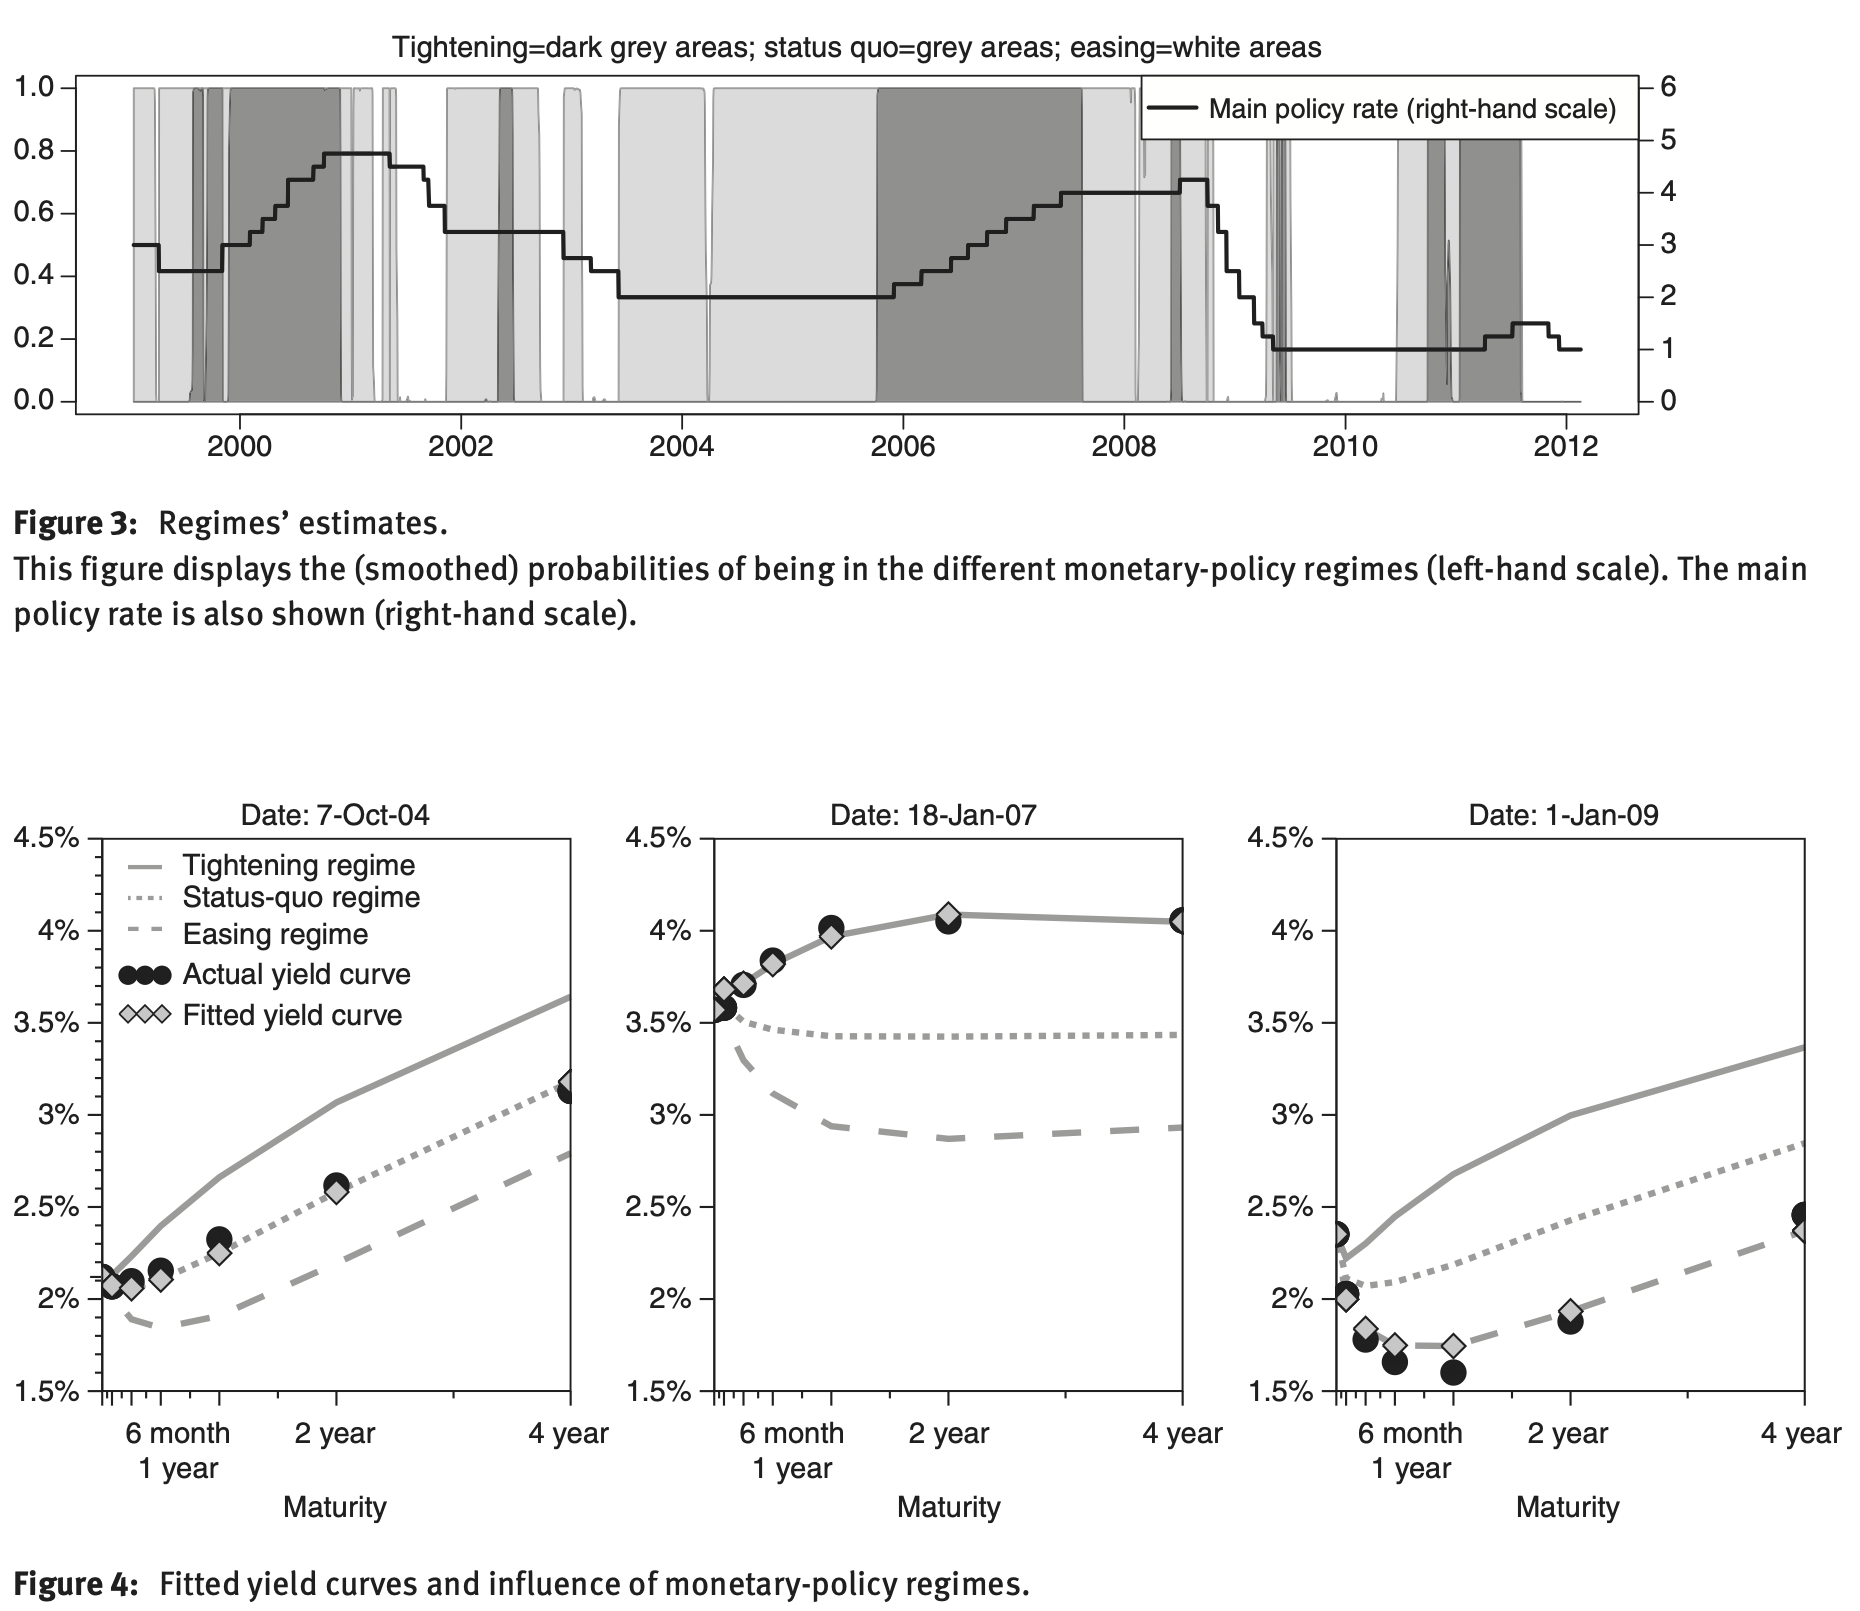
\includegraphics[width=0.95\linewidth]{figures/Fig-SNDE} 

}

\caption{Source: Renne (2017).}\label{fig:figRenne2017}
\end{figure}

\end{example}

\hypertarget{EstimationPersistency}{%
\section{A typical small-sample issue}\label{EstimationPersistency}}

Interest rates are particularly persistent variables. Since affine models eventually lead to linear relationships between state variables and interest rates (see Eq. \eqref{eq:RthAB}), some state variables are also necessarily highly persistent. Accordingly, in small sample, maximum-likelihood estimates of the model parameters are likely to suffer from a downward bias (see, e.g., \citet{Bauer_Rudebusch_Wu_2012} or \citet{Jardet_Monfort_Pegoraro_2013}). This relates to a well-known econometric problem illustrated by Figure \ref{fig:persist1}.

\begin{figure}
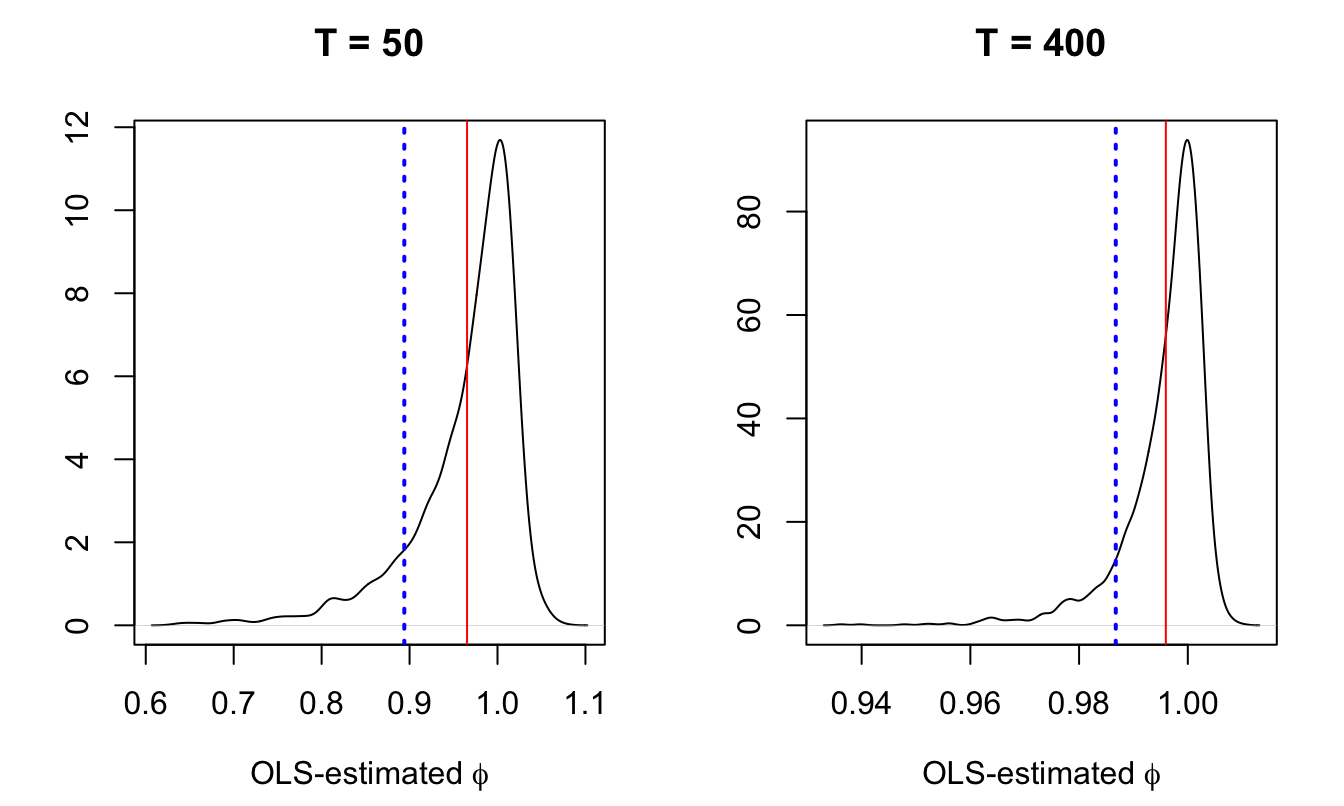
\includegraphics[width=0.95\linewidth]{TSM_files/figure-latex/persist1-1} \caption{1000 random walk samples of size $T$ ($T=50$ for the left plot and $T=400$ for the right plot) have been simulated. For each sample, we run the OLS regression $y_t = \phi y_{t-1} + \varepsilon_t$ to estimate $\phi$ (whose true value is 1). The plots show the distributions (kernel-based estimation) of the estimated $\phi$. The vertical red bar indicate the means of the distributions; the vertical blue line shows the usual bias approximation ($1-5.3/T$).}\label{fig:persist1}
\end{figure}

This small-sample downward bias has dramatic consequences in terms of term premium estimates. For the sake of illustration, consider the following process for the short-term interest rate under the physical measure (monthly frequency):
\[
i_{t+1} = \bar{i} + \phi (i_{t}-\bar{i}) + \sigma \varepsilon_{t+1}, \quad \varepsilon_t \sim \mathcal{N}(0,1).
\]
and the following under the risk-neutral measure:
\[
i_{t+1} = \bar{i}^* + \phi^* (i_{t}-\bar{i}^*) + \sigma \varepsilon^{\mathbb{Q}}_{t+1}, \quad \varepsilon^{\mathbb{Q}}_t \sim \mathcal{N}(0,1).
\]
with \(\bar{i} = 3\%/12\), \(\bar{i}^* = 5\%/12\), \(\phi = 0.98\), \(\phi^*=0.99\), \(\sigma = 0.2\%\).
Assume the estimate of \(\phi\) is downward biased (\(\hat\phi=0.9\)). The influence of that bias on the 10-year term premium is illustrated by Figure \ref{fig:persist2}.

\begin{figure}
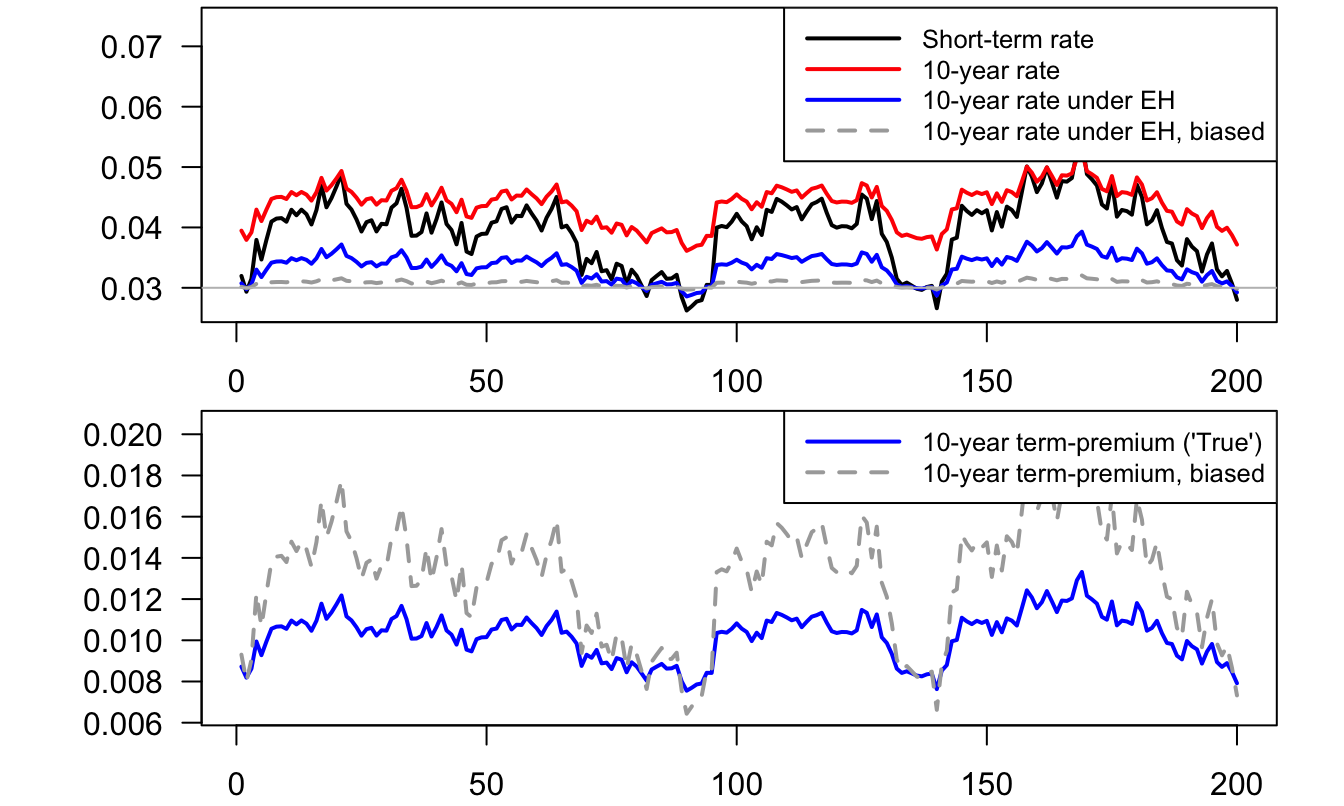
\includegraphics[width=0.95\linewidth]{TSM_files/figure-latex/persist2-1} \caption{This figure illustrates the influence of the downward bias on on estimated term premiums, see the text for more details.}\label{fig:persist2}
\end{figure}

\citet{Kim_Orphanides_2005} have proposed a simple approach to deal with this problem. Their approach consists in adding measurement equations to impose that the model-implied forecasts are---up to some measurement errors---equal to survey-based ones. In their empirical exercise, they use the \href{https://lrus.wolterskluwer.com/store/products/blue-chip-financial-forecasts-prod-ss07418345/paperback-item-1-ss07418345}{Blue Chip Financial Forecasts}. Alternative (publicly available) surveys are: \href{https://www.philadelphiafed.org/research-and-data/real-time-center/survey-of-professional-forecasters}{the Philly Fed Survey of Professional Forecasters} and \href{https://www.ecb.europa.eu/stats/ecb_surveys/survey_of_professional_forecasters/html/index.en.html}{the ECB SPF}.

\citet{Kim_Orphanides_2005} exploit the fact that, in the context of affine models, model-implied forecasts of yields are affine in the state vector (see see Eq. \eqref{eq:condmeanRth}); this implies that their mesurement equations are affine in the state vector, which facilitates the estimation of the latent factors. As shown by Figure \ref{fig:figKimOrph}, their model is able to satisfyingly fit both survey-based forecasts and market yields.

\begin{figure}

{\centering 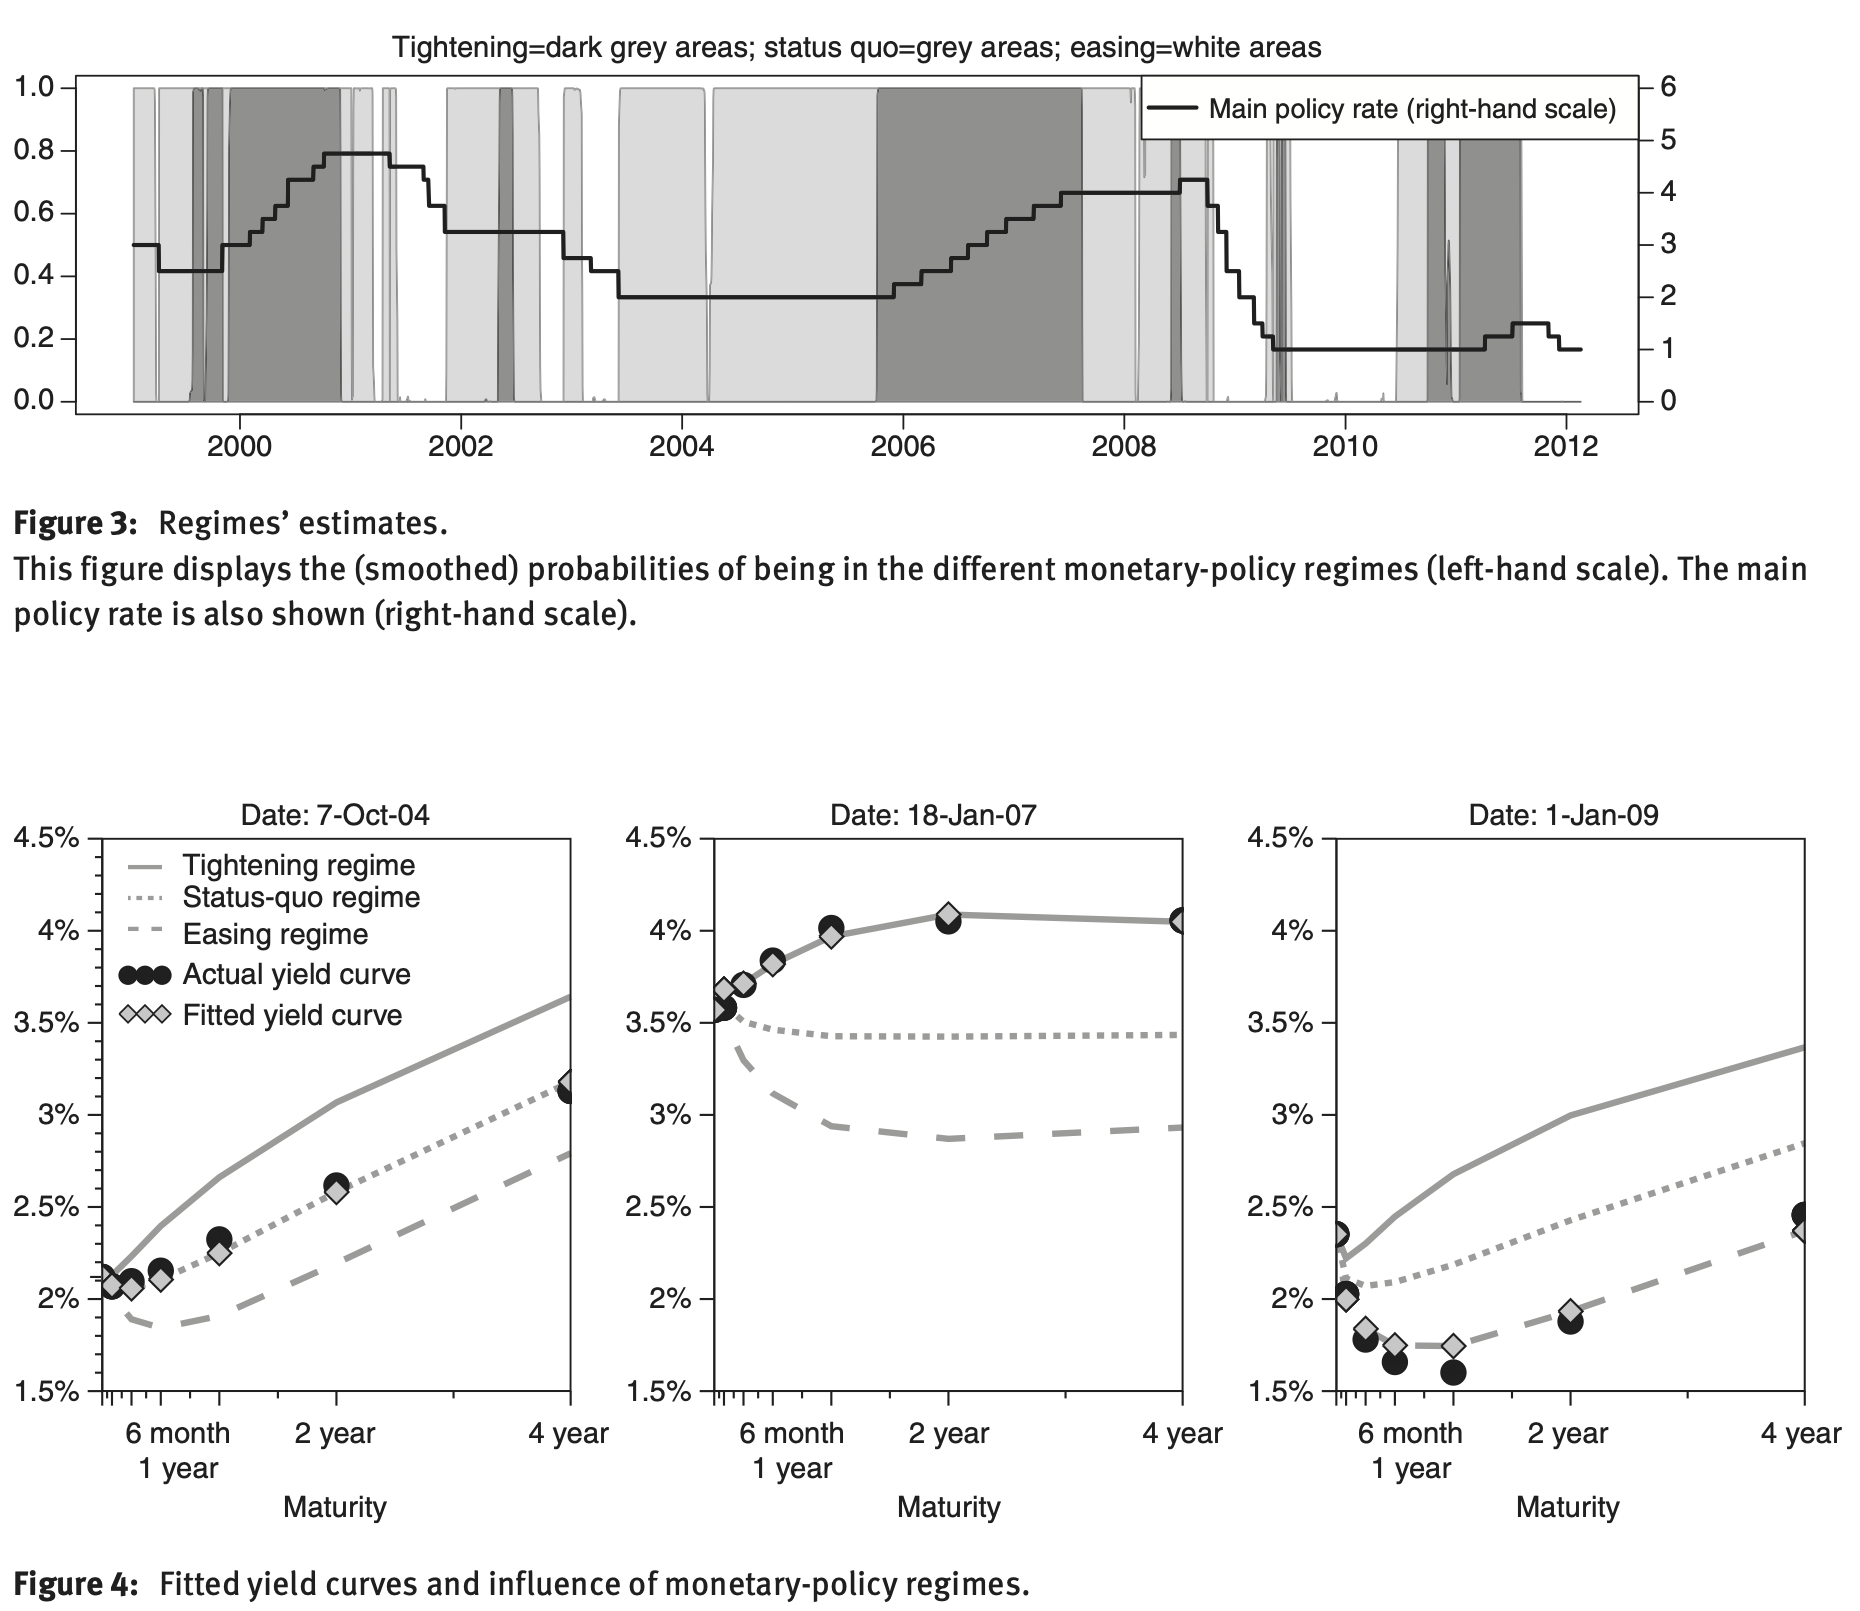
\includegraphics[width=0.95\linewidth]{figures/Fig-SNDE} 

}

\caption{Source: Kim and Orphanides (2005).}\label{fig:figKimOrph}
\end{figure}

\hypertarget{forward-futures-dividends-commodity-pricing-and-convenience-yields}{%
\chapter{Forward, futures, dividends, commodity pricing, and convenience yields}\label{forward-futures-dividends-commodity-pricing-and-convenience-yields}}

\hypertarget{derivatives-written-on-stocks-or-commodities}{%
\section{Derivatives written on stocks or commodities}\label{derivatives-written-on-stocks-or-commodities}}

\hypertarget{FCFPForwards}{%
\subsection{Forward contracts}\label{FCFPForwards}}

Let us denote by \(\underline{w_{t}}\) the information available at \(t\), i.e., \(\underline{w_{t}}= \{w_t,w_{t-1},\dots\}\).

A Forward contract is defined as an agreement, signed at \(t\), to buy/sell an asset (a commodity) at a given delivery date \(T>t\) at a price \(\Phi_{t,T}\), called \emph{delivery price} or \emph{forward price}, decided at \(t\). We denote by \(S_T\) the value of the asset (commodity) at \(T\); this is a function of \(\underline{w_{T}}\). For the buyer, the payoff of the contract at \(T\) is \(S_T - \Phi_{t,T}\).

In this chapter, we denote by \(r_t\) the interest rate between \(t\) and \(t+1\) (known at \(t\)), it is assumed to be a function of \(\underline{w_{t}}\). We also denote by \(B(t_1,t_2-t_1)\) the date-\(t_1\) price of a zero-coupon bond whose value is 1 on \(t_2\).

The following proposition provides an expression for the forward price \(\Phi_{t,T}\):

\begin{proposition}[Forward price]
\protect\hypertarget{prp:fwd}{}\label{prp:fwd}We have:
\begin{eqnarray*}
\Phi_{t,T} & = & \frac{\mathbb{E}_t (\mathcal{M}_{t,t+1}, \ldots, \mathcal{M}_{t-1,T} S_T)}{B(t,T-t)}\\
& = & \frac{\mathbb{E}^{\mathbb{Q}}_t [\exp (-r_t - \ldots - r_{T-1}) S_T]}{B(t,T-t)}.
\end{eqnarray*}
\end{proposition}

\begin{proof}
The price at \(t\) of \(S_T - \Phi_{t,T}\) is zero. Therefore:
\(\mathbb{E}_t (\mathcal{M}_{t,t+1}, \ldots, \mathcal{M}_{t-1,T} S_T) - \Phi_{t,T} \mathbb{E}_t (\mathcal{M}_{t,t+1} \ldots \mathcal{M}_{t-1,T}) = 0\), which gives the result.
\end{proof}

If processes \((r_t)\) and \((S_t)\) are \(\mathbb{Q}\)-independent, then we have
\[
\Phi_{t,T} = \mathbb{E}^{\mathbb{Q}}_t (S_T),
\]
and \(\Phi_{t,T}\) therefore is a \(\mathbb{Q}\)-martingale.

If the asset does not generate any payoff before \(T\) (in the case of shares, there is no dividends), then
\[
\Phi_{t,T} = \frac{S_t}{B(t,T-t)}.
\]
The price at \(s\), with \(t<s<T\), of a forward contract signed at \(t\) is:
\[
(\Phi_{s,T} - \Phi_{t,T}) B (s,T-s),
\]
since the payoff \(S_T - \Phi_{t,T}\) at \(T\) has this price at \(s\).

How are these formulas affected by the presence of dividends? To investigate that, let us introduce additional notations. Denote by \(\tilde{S}_t\) the ex-dividend price at \(t\), and by \(S_t\): the cum-dividend price at \(t\). We have \(S_t = \tilde{S}_t \exp (\delta_t)\), where \(\delta_t\) is the dividend yield (or rate), observed on date \(t\). We get:
\begin{eqnarray*}
\tilde{S}_{T-1} & = & \mathbb{E}_{T-1} (\mathcal{M}_{t-1,T} S_T) \\
\mbox{or } \\
S_{T-1} & = & \mathbb{E}_{T-1} [\mathcal{M}_{t-1,T} \exp (\delta_{T-1})
S_T],
\end{eqnarray*}
and, recursively:
\begin{eqnarray*}
S_t & = & \mathbb{E}_t [\mathcal{M}_{t,t+1} \ldots \mathcal{M}_{t-1,T} \exp (\delta_t + \ldots + \delta_{T-1}) S_T] \\
&=& \mathbb{E}^{\mathbb{Q}}_t [\exp (-r_t \ldots - r_{T-1} + \delta_t + \ldots + \delta_{T-1}) S_T].
\end{eqnarray*}
This shows that the formulas are as in the non-dividend case, except that \(r_t\) is replaced by \(r_t - \delta_t\).

Replacing \(S_t\) by \(\tilde{S} \exp(\delta_t)\) and \(S_T\) by \(\tilde{S}_T \exp (\delta_T)\), we get
\[
\tilde{S}_t = \mathbb{E}^{\mathbb{Q}}_t [\exp (-r_t -\ldots-r_{T-1} + \delta_{t+1} + \ldots + \delta_T) \tilde{S}_T.
\]
When the dividend rate \(\delta_t\) is deterministic, we have:
\[
\Phi_{t,T} = \frac{S_t \exp (-\delta_t - \ldots - \delta_{T-1})}{B(t,T-t)}.
\]
And if \(r_t\) is deterministic too, we have:
\[
\Phi_{t,T} = S_t \exp   (r_t + \ldots + r_{T-1} - \delta_t - \ldots - \delta_{T-1}).
\]

\hypertarget{FCFPFutures}{%
\subsection{Futures contracts, futures prices}\label{FCFPFutures}}

A futures contract is an agreement, signed at \(t\), to buy/sell an asset (a commodity) at given delivery date \(T>t\) at a price \(F_{t,T}\), called \emph{futures price}, decided at \(t\). The difference with forward contract is that both counterparties are required to deposit into a \emph{margin account}, at every trading day \(s>t\), the resettlement payment (\emph{margin call}). The latter is equal to:
\[
\Delta_{s,T} = F_{s,T} - F_{s-1,T} \quad \mbox{(for the buyer)}.
\]

Hence, a futures contract is actually closed out after every day, starts afresh the next day. Its value therefore is zero.

The following proposition values a futures contract.

\begin{proposition}[Pricing futures]
\protect\hypertarget{prp:future}{}\label{prp:future}We have:
\[
F_{t,T} = \mathbb{E}^{\mathbb{Q}}_t (S_T),
\]
that is \(F_{t,T}\) is a \(\mathbb{Q}\)-martingale, and \(\Delta_{t,T}\) is a \(\mathbb{Q}\)-martingale difference.
\end{proposition}

\begin{proof}
At each date \(s\ge t\), after the deposit of the resettlement payment, there is a new contract valued zero and paying \(F_{s+1,T} - F_{s,T}\) at \(s+1\) (and providing another zero valued contract at \(s+1\)). Therefore \(0 = \mathbb{E}^{\mathbb{Q}}_s [\exp (-r_s) (F_{s+1,T} - F_{s,T})]\), and \(0 = \mathbb{E}^{\mathbb{Q}}_s (F_{s+1,T} - F_{s,T})\) since \(\exp (-r_s)\) is known at \(s\). Hence \(F_{s,T} = \mathbb{E}^{\mathbb{Q}}_s (F_{s+1,T})\), and the results follows from \(F_{T,T} = S_T\).
\end{proof}

\begin{proposition}[Forward-Futures deviation]
\protect\hypertarget{prp:FFdeviation}{}\label{prp:FFdeviation}We have:
\[
\Phi_{t,T} - F_{t,T} = \frac{\mathbb{C}ov^{\mathbb{Q}}_t \left[\prod^{T-1}_{s=t} \exp (-r_s), S_T\right]}{B(t,T-t)}.
\]
\end{proposition}

\begin{proof}
We have:
\begin{eqnarray*}
\Phi_{t,T} - F_{t,T} & = & \mathbb{E}^{\mathbb{Q}}_t \left[\frac{\prod^{T-1}_{s=t} \exp (-r_s) S_T }{B(t,T-t)}- S_T\right] \\
&=& \frac{\mathbb{E}^{\mathbb{Q}}_t \left[\prod^{T-1}_{s=t} \exp (-r_s) S_T\right] - \mathbb{E}^{\mathbb{Q}}_t \left[\prod^{T-1}_{s=t} \exp (-r_s)\right] \mathbb{E}^{\mathbb{Q}}_t (S_T)}{B(t,T-t)} \\
&=&\frac{cov^{\mathbb{Q}}_t \left[\prod^{T-1}_{s=t} \exp (-r_s), S_T)\right]}{B(t,T-t)}. \end{eqnarray*}
\end{proof}

Hence, \(\Phi_{t,T} = F_{t,T}\) if, and only if, \(\prod^{T-1}_{s=t} \exp (-r_s)\) and \(S_T\) are conditionally uncorrelated under \(\mathbb{Q}\). It is true, in particular, in the case of deterministic short rates.

\hypertarget{FCFPConvenience}{%
\subsection{Convenience yields}\label{FCFPConvenience}}

A convenience yield is defined as the net benefit associated with holding a physical asset (rather than a forward or futures contract). It is \emph{net} in the sense that it is equal to the positive gain of holding minus potential storage costs.

The notion of convenience yield is relevant only for storable commodities (not, e.g., for electricity). It can be positive or negative. The notion of convenience yield is mathematically similar to that of a dividend yield (but can be \(<0\), and is often latent).

In the following, we denote the convenience yield by \(c_t\). The price is here the cum-convenience yield price.

Let us first consider the case where \(r_t\) and \(c_t\) are deterministic. We have:
\[
\Phi_{t,T} = F_{t,T} = S_t \exp (r_t + \ldots + r_{T-1} - c_t - \ldots - c_{T-1}).
\]
Moreover, if \(r_t\) and \(c_t\) are time independent, we get:
\[
\Phi_{t,T} = F_{t,T} = S_t \exp [(T-t)(r-c)].
\]
If \(r>c\), the forward curve is an increasing function of matuerity \(T\); this is known as a situation of \emph{contango}. If \(r<c\), the forward curve is a decreasing function of maturity \(T\), know as a situation of \emph{backwardation}.

Let us turn to the situation where \(c_t\) is stochastic. We have:
\begin{eqnarray}
\Phi_{t,T} &=& \mathbb{E}^{\mathbb{Q}}_t [\exp (-r_t - \ldots - r_{T-1}) S_T]/B(t,T-t) \label{eq:convenience1}\\
F_{t,T} &=& \mathbb{E}^{\mathbb{Q}}_t (S_T) \label{eq:convenience2}\\
S_t &=& \mathbb{E}^{\mathbb{Q}}_t [\exp (-r_t - \ldots - r_{T-1} + c_t + \ldots + c_{T-1}) S_T] \label{eq:convenience3}.
\end{eqnarray}
Going further necessitates a joint modelling---at least under \(\mathbb{Q}\)---of \(S_t\) (or \(s_t = \log S_t\)), \(c_t\) (convenience yield), and \(r_t\) (short rate).

\begin{quote}
In the case of a \textbf{nonstorable commodity}, there is no convenience yield. If, moreover \(r_t\) deterministic, \(\Phi_{t,T} = F_{t,T} = \mathbb{E}^{\mathbb{Q}}_t (S_T)\), but since \eqref{eq:convenience3} is not valid we do not have \(S_t = B(t,T) \mathbb{E}^{\mathbb{Q}}_t (S_T)\) and therefore we do not have \(\Phi_{t,T} = S_t / B(t,T)\).
\end{quote}

\begin{quote}
In the case of a \textbf{storable commodity}, the price ex-convenience yield at \(t\), i.e.~\(S_t \exp (-c_t)\), is the price at \(t\) of \(S_{t+1}\):
\begin{eqnarray}
S_t \exp (-c_t) &=& \exp (-r_t) \mathbb{E}^{\mathbb{Q}}_t (S_{t+1}) \nonumber\\
\mathbb{E}^{\mathbb{Q}}_t (S_{t+1}) & = & S_t \exp (r_t - c_t) \label{eq:convenience4} \\
\mathbb{E}^{\mathbb{Q}}_t \exp (s_{t+1}) &=& \exp(s_t+r_t-c_t). \nonumber
\end{eqnarray}
Or if \(y_{t+1} = \log \frac{S_{t+1}}{S_t}\) denotes the (geometric) return, then:
\[
\mathbb{E}^{\mathbb{Q}}_t \exp (y_{t+1}) = \exp (r_t - c_t).
\]
Eq. \eqref{eq:convenience3} is automatically satisfied (using \eqref{eq:convenience4} recursively).
\end{quote}

\hypertarget{FCFPPricingRN}{%
\subsection{Pricing with affine models}\label{FCFPPricingRN}}

In this section, we consider a storable commodity. The state vector is as follows:
\[
w_t = (s_t, c_t, r_t, x'_t)',
\]
where \(s_t = \log S_t\), and where \(x_t\) is a vector of additional factors. We further assume that \(w_t\) is a \(\mathbb{Q}\)-affine process, that is:
\[
\mathbb{E}^{\mathbb{Q}}_t \exp (u' w_{t+1}) = \exp [a' (u) w_t + b(u)].
\]
Since \(S_{t+1} = \exp (e_1' w_{t+1})\), Internal Consistency Constraints (ICCs) apply (see Subsection \ref{DirectModeling}), and we have:
\begin{eqnarray*}
&&\mathbb{E}^{\mathbb{Q}}_t \exp (s_{t+1}) = \exp (s_t-c_t+r_t)\\
&\Leftrightarrow& \mathbb{E}^{\mathbb{Q}}_t \exp (e_1' w_{t+1}) = \exp [(e_1 - e_2 + e_3)' w_t]\\
&\Leftrightarrow& \left\{\begin{array}{lcl}
a(e_1) &=& e_1 - e_2 + e_3 \\
b(e_1) &=&0.
\end{array} \right.
\end{eqnarray*}

\begin{quote}
If the commodity is non-storable, there are no \(c_t\), and no ICCs.
\end{quote}

Eqs. \eqref{eq:convenience1} and \eqref{eq:convenience2} give:
\begin{eqnarray*}
\Phi_{t,T} & = & \frac{\mathbb{E}^{\mathbb{Q}}_t [\exp (-r_t - \ldots - r_{t-1} + s_T)]}{\mathbb{E}^{\mathbb{Q}}_t [\exp (-r_t - \ldots - r_{T-1})]} \\
F_{t,T} & = & \mathbb{E}^{\mathbb{Q}}_t [\exp (s_T)].
\end{eqnarray*}
Using the multi-horizon Laplace transforms of \(w_t = (s_t, c_t, r_t, x^{'}_t)'\), we get quasi explicit formulas for these prices (as they are exponential affine in future values of \(w_t\), which is an affine process).

\hypertarget{historical-dynamics}{%
\subsection{Historical dynamics}\label{historical-dynamics}}

Using the notation of Subsection \ref{PricingAffine}, assume the SDF is of the form:
\[
\mathcal{M}_{t,t+1} (\underline{w_{t+1}}) = \exp \left[-r_t + \alpha'_t w_{t+1} + \psi^{\mathbb{Q}}_t (-\alpha_t)\right],
\]
such that
\[
\mathbb{E}^{\mathbb{Q}}_t (\mathcal{M}_{t,t+1}^{-1}) = \exp (r_t).
\]

The historical dynamics of \(w_t\) is defined through:
\[
\psi_t (u) = \psi^{\mathbb{Q}}_t (u-\alpha_t) - \psi^{\mathbb{Q}}_t(-\alpha_t).
\]

\begin{quote}
There is no constraint on \(\alpha_t\), which can be used, e.g., to specify some forms of seasonality (see Example \ref{exm:FCFPGaussian}).
\end{quote}

\begin{example}[A Gaussian VAR model]
\protect\hypertarget{exm:FCFPGaussian}{}\label{exm:FCFPGaussian}Consider the state vector \(w_t = (s_t, c_t, r_t)'\), whose R.N. dynamics reads:
\[
w_{t+1} = A_0 + A_1 w_t + \varepsilon_{t+1}, \quad \varepsilon_{t+1} \sim  i.i.d. \mathcal{N}(0,\Sigma) \mbox{ under }\mathbb{Q}.
\]
We then have (see Example \ref{exm:GAR1}):
\begin{eqnarray*}
\mathbb{E}_t \exp (u' w_{t+1}) &=& \exp \left[u' (A_0 + A_1 w_t) + \frac{1}{2} u' \Sigma u\right] \\
\Rightarrow &&
\left\{
\begin{array}{ccl}
a(u) &=&A^{'}_1 u \\
b(u) & =& A'_0 u + \frac{1}{2} u' \Sigma u. \end{array} \right.
\end{eqnarray*}
Decompose \(A_0\) and \(A_1\) as follows:
\begin{eqnarray*}
A_0 &=& \left(
\begin{array}{c} A_{01} \\ \tilde{A}_0
\end{array}
\right), \quad A_1 = \left(
\begin{array}{c} A_{11} \\
\tilde{A}_1
\end{array}
\right).
\end{eqnarray*}
If the considered commodity is storable, we have the following ICCs (no constraint otherwise):
\[
\left\{
\begin{array}{ccl}
a (e_1) & = & e_1 - e_2 + e_3 \\
b (e_1) &=& 0. \end{array}
\right.
\]
Therefore, the first row of \(A_1\) is \(A_{11} = e_1'- e_2' + e_3'\), the first element of \(A_0\) is \(A_{01} = -\frac{1}{2}\sigma^2_1\) (\(\sigma^2_1\) being the conditional variance of \(s_{t+1}\)).

In other words the \(\mathbb{Q}\)-VAR is:
\[
\left\{\begin{array}{cclcc} s_{t+1} & = & -\frac{1}{2}
\sigma^2_1 + s_t - c_t + r_t &+& \varepsilon_{1,t+1} \\
\left(\begin{array}{c} c_{t+1} \\ r_{t+1} \end{array} \right) & = &
\tilde{A}_0 + \tilde{A}_1 w_t &+& \left(\begin{array}{c} \varepsilon_{2,t+1} \\
\varepsilon_{3,t+1} \end{array} \right),
\end{array} \right.
\]
where \(\tilde{A}_0\) and \(\tilde{A}_1\) are not constrained.

Noting \(y_{t+1} = \log (S_{t+1}/S_t) = s_{t+1} - s_t\), this implies that
\[
\mathbb{E}^{\mathbb{Q}}_t y_{t+1} = r_t - c_t - \frac{1}{2} \sigma^2_1.
\]
Hence, \(y_{t+1} - r_t + c_t + \frac{1}{2} \sigma^2_1\) is a \(\mathbb{Q}\)-martingale difference.

The historical dynamics of the state vector is as follows:
\[
\begin{array}{lcl}
\psi_t (u) & = & \psi^{\mathbb{Q}}_t (u-\alpha_t) - \psi^{\mathbb{Q}}_t (- \alpha_t) \\
&=& u' (A_0 + A_1 w_t) + \frac{1}{2} (u-\alpha_t)' \Sigma (u-\alpha_t)- \frac{1}{2} \alpha'_t
\Sigma \alpha_t \\
&=&u' (A_0 + A_1 w_t) - u' \Sigma \alpha_t + \frac{1}{2} u' \Sigma u.
\end{array}
\]
If we take \(\alpha_t = \alpha_0 + \alpha_1 w_t\), we get:
\begin{eqnarray*}
\psi_t (u) &=& u' [A_0 - \Sigma \alpha_0 + (A_1 - \Sigma \alpha_1) w_t] + \frac{1}{2} u' \Sigma u \\
\Rightarrow  w_{t+1} &=& A_0 - \Sigma \alpha_0 + (A_1 - \Sigma \alpha_1) w_t + \xi_t,\\
&& \xi_t \sim  i.i.d.   \mathcal{N}(0,\Sigma)\; \mbox{under}\;\mathbb{P}.
\end{eqnarray*}
Hence, any VAR(1), with same \(\Sigma\), can be reached.

We can also take a time-varying specification for \(\alpha_t\), of the form \(\alpha_t = \alpha_{0t} + \alpha_1 w_t\). We then get the historical dynamics:
\[
w_{t+1} = A_{0} - \Sigma \alpha_{0t} + (A_1 - \Sigma \alpha_1) w_t + \xi_{t+1}
\]
We can for instance choose \(\alpha_{0t}\) such that: \(A_{0} - \Sigma \alpha_{0t} = \left( \begin{array}{c} \mu_{1t} \\ \mu_2 \\ \mu_3 \end{array}\right)\), where \(\mu_{1t}\), \(\mu_2\), and \(\mu_3\) are given.
In particular:
\begin{eqnarray*}
s_{t+1} & = & \mu_{1t} + (A_{11} - \Sigma_1 \alpha_1) w_t + \xi_{1,t+1} \\
& = & \mu_{1t} + \bar{A}_{11} w_t + \xi_{1,t+1}\; \mbox{(say)}, \;
\end{eqnarray*}
where \(\bar{A}_{11}\) is not constrained, or:
\[
s_{t+1} - \nu_{t+1} = \mu_1 + \bar{A}_{11,1} (s_t - \nu_t) + \bar{A}_{11,2} c_t + \bar{A}_{11,3} r_t + \xi_{1,t+1}
\]
with
\[
\mu_{1t} = \mu_1 + \nu_{t+1} - \bar{A}_{11,1} \nu_t.
\]
In other words any historical seasonal function \(\nu_t\) can be reached by choosing \(\mu_{1t}\), i.e., \(\alpha_{0t}\).
\end{example}

\begin{example}[Schwartz (1997)]
\protect\hypertarget{exm:Schwartz1997}{}\label{exm:Schwartz1997}

\citet{Schwartz_1997} proposes three models whose discrete-time versions are:

\begin{itemize}
\tightlist
\item
  \textbf{Model 1}:
  \begin{eqnarray*}
  \mathbb{P}&:& s_{t+1} = a_0 + a_1 s_t + \sigma \varepsilon_{t+1}, \; \; \; \varepsilon_t \stackrel{\mathbb{P}}{\sim}  i.i.d. \mathcal{N}(0,1) \\
  \mathbb{Q} &:& s_{t+1} = a^*_0 + a_1 s_t + \sigma \xi_{t+1}, \; \; \; \xi_{t} \stackrel{\mathbb{Q}}{\sim}  i.i.d. \mathcal{N}(0,1).
  \end{eqnarray*}
\item
  \textbf{Model 2}:
  \begin{eqnarray*}
  \mathbb{P}&:& s_{t+1} = a_{10} + s_t - c_t + \sigma_1 \varepsilon_{1,t+1}\\
  && c_{t+1} = a_{20} + a_{21} c_t + \sigma_2 \varepsilon_{2,t+1}\hspace{1cm} corr (\varepsilon_{1t}, \varepsilon_{2,t}) = \rho \\
  \mathbb{Q}&:& s_{t+1} = r - \frac{\sigma^2_1}{2} + s_t - c_t + \sigma_1  \xi_{1,t+1} \\
  && c_{t+1} = a^*_{20} + a_{21} c_t + \sigma_2 \xi_{2,t+1} \hspace{1cm} corr (\xi_{1t}, \xi_{2t}) = \rho.
  \end{eqnarray*}
\item
  \textbf{Model 3}:
  \begin{eqnarray*}
  \mathbb{P}&:& s_{t+1} = a_{10} + s_t - c_t + r_t + \sigma_1 \varepsilon_{1,t+1} \\
  && c_{t+1}= a_{20} + a_{21} c_t + \sigma_2 \varepsilon_{2,t+1} \\
  && r_{r+1} = a_{30} + a_{31} r_t + \sigma_3 \varepsilon_{3,t+1} \\
  \mathbb{Q}&:& s_{t+1} = -\frac{\sigma^2_1}{2} + s_t - c_t + r_t + \sigma_1 \xi_{1,t+1}\\
  &&c_{t+1} = a^*_{20} + a_{21} c_t + \sigma_2 \xi_{2,t+1} \\
  &&r_{t+1} = a_{30} + a_{31} r_t + \sigma_3 \xi_{3,t+1},
  \end{eqnarray*}
  with \(\mathbb{C}orr(\varepsilon_{1t}, \varepsilon_{2t}) = \rho_1\), \(\mathbb{C}orr(\varepsilon_{2t}, \varepsilon_{3t}) = \rho_2\), \(\mathbb{C}orr(\varepsilon_{1t}, \varepsilon_{3t}) = \rho_3\), and idem for the \(\xi_{it}\)'s. (All shocks are \(\mathcal{N}(0,1)\).)
\end{itemize}

In these models, \(\log F_{t,T}\) is an affine function of \(\{s_t, c_t, r_t\}\).

From an estimation point of view, \(s_t\) and \(c_t\) are latent. The parameters are estimated by the ML method, the likelihood functions being computed by the Kalman filter (see Subsection \ref{Estimation:KF}). The state variable is \(s_t\) in Model 1, and \(\{s_t, c_t\}\) in Models 2 and 3. (The \(\mathbb{P}\) and \(\mathbb{Q}\) dynamics of \(r_t\) are estimated separately.)

As can be seen in the previous equations, constraints are imposed between the \(\mathbb{P}\) and \(\mathbb{Q}\) parameters; this is to help the identification of the model parameters.

\begin{figure}

{\centering 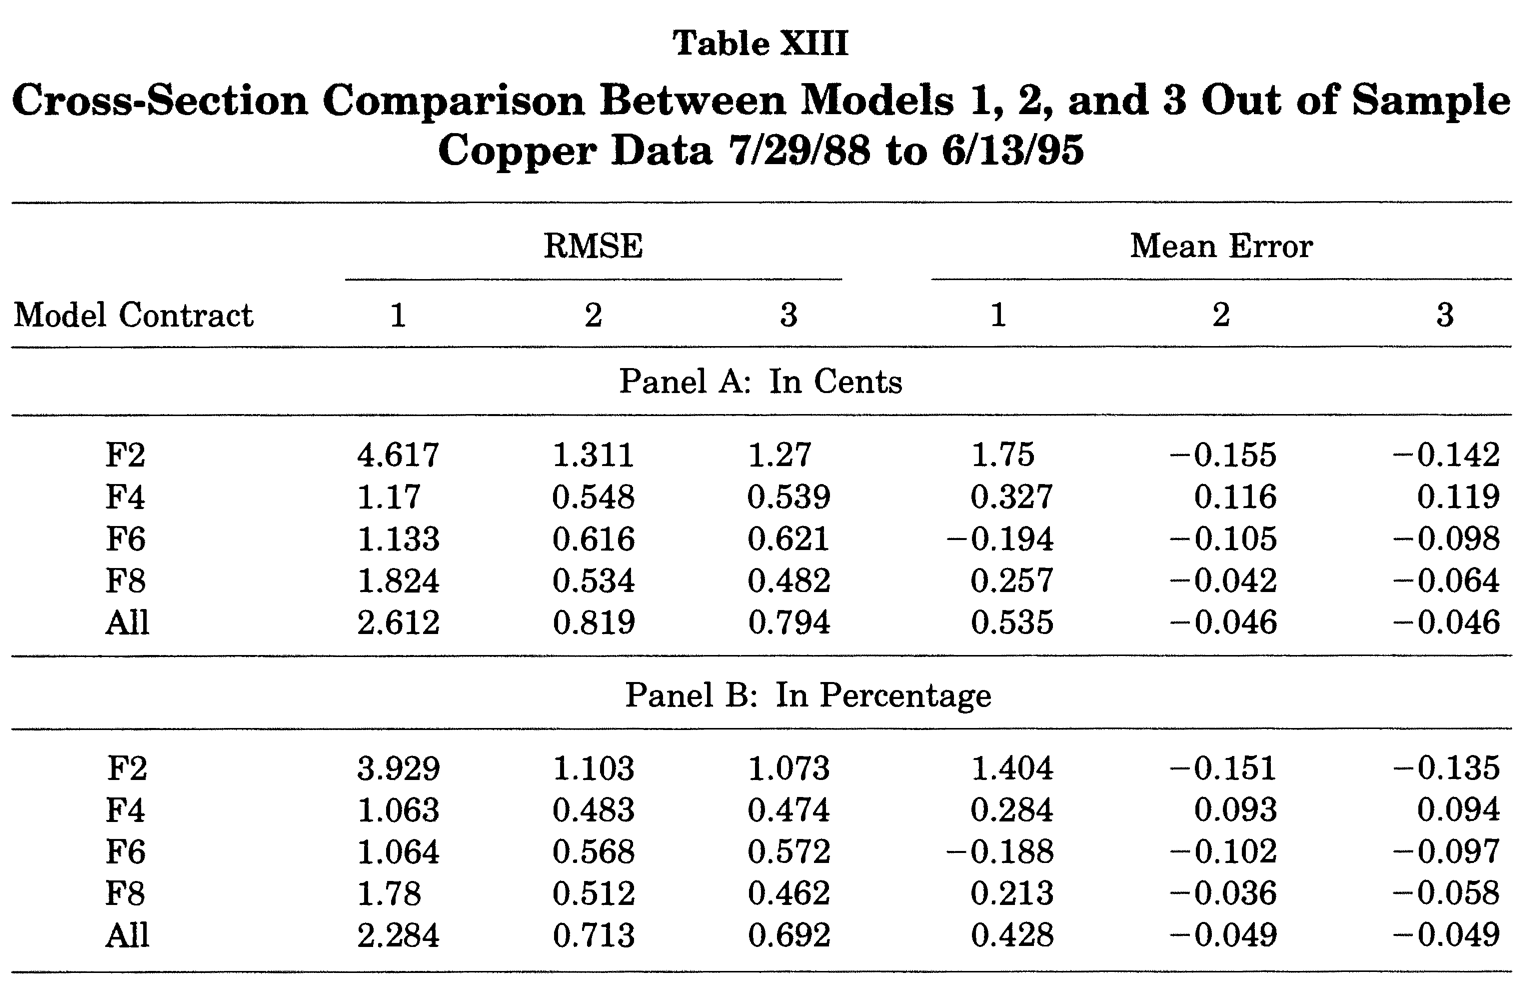
\includegraphics[width=0.95\linewidth]{figures/Tab2_Schwartz} 

}

\caption{Out of sample means for maturities not used at the  estimation stage. F1 contract : the closest to maturity F2 : the second contract to maturity and so one. Source: Schwartz (1997).}\label{fig:Schwartz2}
\end{figure}

\end{example}

\hypertarget{interest-rate-swaps-and-forward-contracts}{%
\section{Interest-rate swaps and forward contracts}\label{interest-rate-swaps-and-forward-contracts}}

\hypertarget{Swaps}{%
\subsection{Swap rates}\label{Swaps}}

\begin{definition}[Interest Rate Swap (IRS)]
\protect\hypertarget{def:swap}{}\label{def:swap}In an Interest Rate Swap (IRS), a \emph{fixed-rate payer} agrees to provide the \emph{fixed-rate receiver} with a sequence of cash flows that are determined at the negotiation date of the swap, and at predetermined dates. These cash flows constitute the \emph{fixed leg} of the swap. Conversely, the fixed-rate receiver provides the fixed-rate payer with cash-flows that depend on future values of a reference rate; this is the \emph{floating rate} of the swap.

More precisely, the dates of payment are of the form \(t+ \tau\), \(t + 2\tau\), \dots, \(t + n\tau\), where \(\tau\) is a period expressed in years (typically 1/2 or 1/4) and \(n\) is the number of payments. The maturity, or \emph{tenor}, of the swap contract is \(h = n \tau\).

The payoffs of the fixed leg are \(\tau S\), where \(S\) is the annualized payment (or \emph{swap rate}). On date \(t+j\tau\), the payoff of the floating leg is \(\tau L(t+(j-1)\tau,\tau)\), where \(L\), the annualized linear rate is given by:
\[
L(t+(j-1)\tau,\tau) = \frac{1 - B(t+(j-1)\tau,\tau)}{\tau B(t+(j-1)\tau,\tau)},
\]
where \(B(t+(j-1)\tau,\tau)\) is the price, at date \(t+(j-1)\tau\) of a bond of maturity \(\tau\).

On the negotiation date, the values of the fixed and floating legs are identical, so that the value of the swap is zero.
\end{definition}

\begin{proposition}[Swap rate formula]
\protect\hypertarget{prp:swap}{}\label{prp:swap}The swap rate \(S(t,h)\), as defined in Def. \ref{def:swap} satisfies:
\begin{equation}
\boxed{S(t,h) = \frac{1 - B(t,h)}{\tau \sum_{j=1}^{h/\tau}  B(t,j\tau)}.}\label{eq:swap}
\end{equation}
\end{proposition}

\begin{proof}
At \(t\), the price of the fixed leg is:
\[
\sum_{j=1}^n \tau S B(t,j\tau).
\]
Let us turn to the price of the floating leg. The payoff at date \(t+j\tau\), that is \(\frac{1 - B(t+(j-1)\tau,\tau)}{B(t+(j-1)\tau,\tau)}\) is known on date \(t+(j-1)\tau\), so its price at date \(t+(j-1)\tau\) is \(1 - B(t+(j-1)\tau,\tau)\), and its price at \(t\) therefore is \(B(t,(j-1)\tau) - B(t,j\tau)\). Summing over \(j=1,\dots,n\), the date-\(t\) price of the floating leg is \(1 - B(t,n\tau)\) (independent of the payment dates).

Since the price of the contract is zero at date \(t\) (by definition of the swap), we must have:
\[
\sum_{j=1}^n \tau S B(t,j\tau) = 1 - B(t,n\tau),
\]
which gives \eqref{eq:swap}.
\end{proof}

\begin{quote}
Note that all the terms appearing in the previous formula are available in closed-form in the context of an affine model (see Example \ref{exm:nominalBth}).
\end{quote}

\begin{quote}
Eq. \eqref{eq:swap} also shows that we have \(100\% = B(t,h) + S(t,h) \tau \sum_{j=1}^{h/\tau} B(t,j\tau)\). This equation means that the swap rate \(S(t,h)\) is homogenous to the yield-to-maturity of a bond valued at par (\(100\%\)), whose coupons are equal to \(S(t,h) \tau\). (The coupons are paid on \(\{t+\tau,\dots,t+n\tau\}\).) In other words, a swap yield is homogenous to a \emph{par yield}.
\end{quote}

\hypertarget{FWD}{%
\subsection{Forward rates}\label{FWD}}

\begin{definition}[Forward Rate Agreement (FRA)]
\protect\hypertarget{def:FWD}{}\label{def:FWD}An interest rate forward contract is a contract in which the rate to be paid or received on a specific obligation for a set period, beginning in the future, is set at contract initiation.

Denote by \(f(t,h_1,h_2)\) the forward interest rate, set on date \(t\), for the period between \(t+h_1\) and \(t+h_2\). One of the two counterparties will pay \(\exp(-f(t,h_1,h_2)(h_2 - h_1))\) on date \(t+h_1\), and receive one on date \(t+h_2\).
\end{definition}

\begin{proposition}[Forward rate formula]
\protect\hypertarget{prp:fwd}{}\label{prp:fwd}The forward rate defined in Def. \ref{def:FWD} satisfies:
\begin{equation}
\boxed{f(t,h_1,h_2) = \frac{h_2 R(t,h_2) - h_1 R(t,h_1)}{h_2 - h_1},}\label{eq:forward}
\end{equation}
where \(R_{t,h}\) denotes the date-\(t\) continuously-compounded yield of maturity \(h\).
\end{proposition}

\begin{proof}
Consider two strategies (decided on date \(t\)):

\begin{enumerate}
\def\labelenumi{\arabic{enumi}.}
\tightlist
\item
  Buy a zero-coupon bond of maturity \(h_2\) (price \(B(t,h_2)\)) and sell zero-coupon bonds of maturity \(h_1\) for the same amount (yielding a payoff of \(B(t,h_2)/B(t,h_1)\) on date \(t+h_1\)).
\item
  Enter a forward rate agreement between dates \(t+h_1\) and \(t+h_2\), whereby you receive 1 on date \(t+h_2\).
\end{enumerate}

These two strategies deliver the same payoffs on date \(t\) (the payoff is zero) and on date \(t+h_2\) (the payoff is 1). By absence of arbitrage, the payoffs on date \(t+h_1\) have to be the same. Therefore
\begin{eqnarray*}
\exp(-(h_2 - h_1)f(t,h_1,h_2)) &=& B(t,h_2)/B(t,h_1) \\
\Rightarrow f(t,h_1,h_2) &=& \frac{1}{h_2 - h_1}(\log[B(t,h_1)] - \log[B(t,h_2)]),
\end{eqnarray*}
which gives \eqref{eq:forward}.
\end{proof}

\begin{quote}
In an affine model (where \(R(t,h)\) is an affine function of the state vector \(w_t\)), forward rates are linear in the state vector \(w_t\).
\end{quote}

\hypertarget{CreditLiRisks}{%
\chapter{Credit and liquidity risks}\label{CreditLiRisks}}

\hypertarget{CreditNotations}{%
\section{Notations}\label{CreditNotations}}

The information of the investor at date \(t\) is still denoted by \(\underline{w_t} = (w_t',w_{t-1}',\dots, w_1 ') '\), but \(w_t\) now comprises a new subsector, namely \(d_t\), that keeps track of the ``default'' status of some creditors. Formally, \(w_t = (y_t',d_t')'\), where \(y_t\) is a \(n_y\)-dimensional vector of common factors, and \(d_t = (d_{1, t} , \dots, d_{E, t}) '\) a \(E\)-dimensional vector of binary variables representing the possible default of entities \(e \in \{1, \dots,E\}\). Vector \(w_t\) is \(K\)-dimensional, that is \(K = n_y + E\).

By convention:

\begin{itemize}
\tightlist
\item
  \(d_{e, t} = 1\) if entity \(e\) is in default status at time \(t\),
\item
  \(d_{e, t} = 0\) if entity \(e\) is not in default status at time \(t\).
\end{itemize}

We assume that the process \(\{w_t\}\) is Markov. Formally, its historical (\(\mathbb{P}\)) dynamics is defined by the conditional densities:
\[
f (y_t  |  w_{t-1}) \mbox{ and }p ( d_t  |  y_t, w_{t-1} ).
\]

In what follows, we assume that the default state is absorbing:

\begin{hypothesis}[absorbing defaults]
\protect\hypertarget{hyp:A4}{}\label{hyp:A4}The default event is an absorbing state. Formally: \(p_e ( 0 | y_t, w_{t-1}, d_{e,t-1}=1 ) = 0\).
\end{hypothesis}

The \emph{survival probability} is defined as follows:
\begin{equation}
p_e ( 0  |  y_t, w_{t-1}, d_{e,t-1}=0 ) = \exp[-\underbrace{\lambda_e ( y_t, w_{t-1})}_{\color{blue}{\mbox{default intensity}}}].\label{eq:survival}
\end{equation}

It is easily checked that \(\lambda_e ( y_t, w_{t-1})\) is close to the conditional probability of default when it is small.

\hypertarget{CreditStandard}{%
\section{Pricing under standard assumptions}\label{CreditStandard}}

To start with, we will consider the pricing of defaultable bonds under assumptions that are standard in the literature, a framework that we call the \emph{classical credit-risk framework}. These assumptions---namely \ref{hyp:A1} and \ref{hyp:A3}---lead to simple formulas. We will investigate further what happens when these assumptions are relaxed (Subsection \ref{Creditrelaxing}).

\begin{hypothesis}[Non-systemic entity]
\protect\hypertarget{hyp:A1}{}\label{hyp:A1}\(\{d_t\}\) does not Granger-cause \(\{y_t\}\), in the sense that:
\[
f(y_t|w_{t-1}) = f(y_t|y_{t-1}).
\]
\end{hypothesis}

In other words, under Hypothesis \ref{hyp:A1}, \(y_t\) is exogenous to \(d_t\).

\begin{hypothesis}[Unpriced credit events]
\protect\hypertarget{hyp:A3}{}\label{hyp:A3}The default events (or credit events) are not priced, in the sense that:
\begin{equation*}
\mathcal{M}_{t-1, t}( w_t, w_{t-1}) = \mathcal{M}_{t-1, t}( y_t, y_{t-1}) .
\end{equation*}
\end{hypothesis}

In other words, under Hypothesis \ref{hyp:A3}, defaults do not affect the SDF conditionally on \(\underline{y_t}\).

Hypothesis \ref{hyp:A3} also implies that the short-term risk-free rate \(i_t=-\log\mathbb{E}_t(\mathcal{M}_{t,t+1})\) depends on \(\underline{y_t}\) (but not on \(d_t\)).

Figure \ref{fig:classical} provides a graphical representation of the causality scheme in the classical credit-risk framework.

\begin{figure}

{\centering 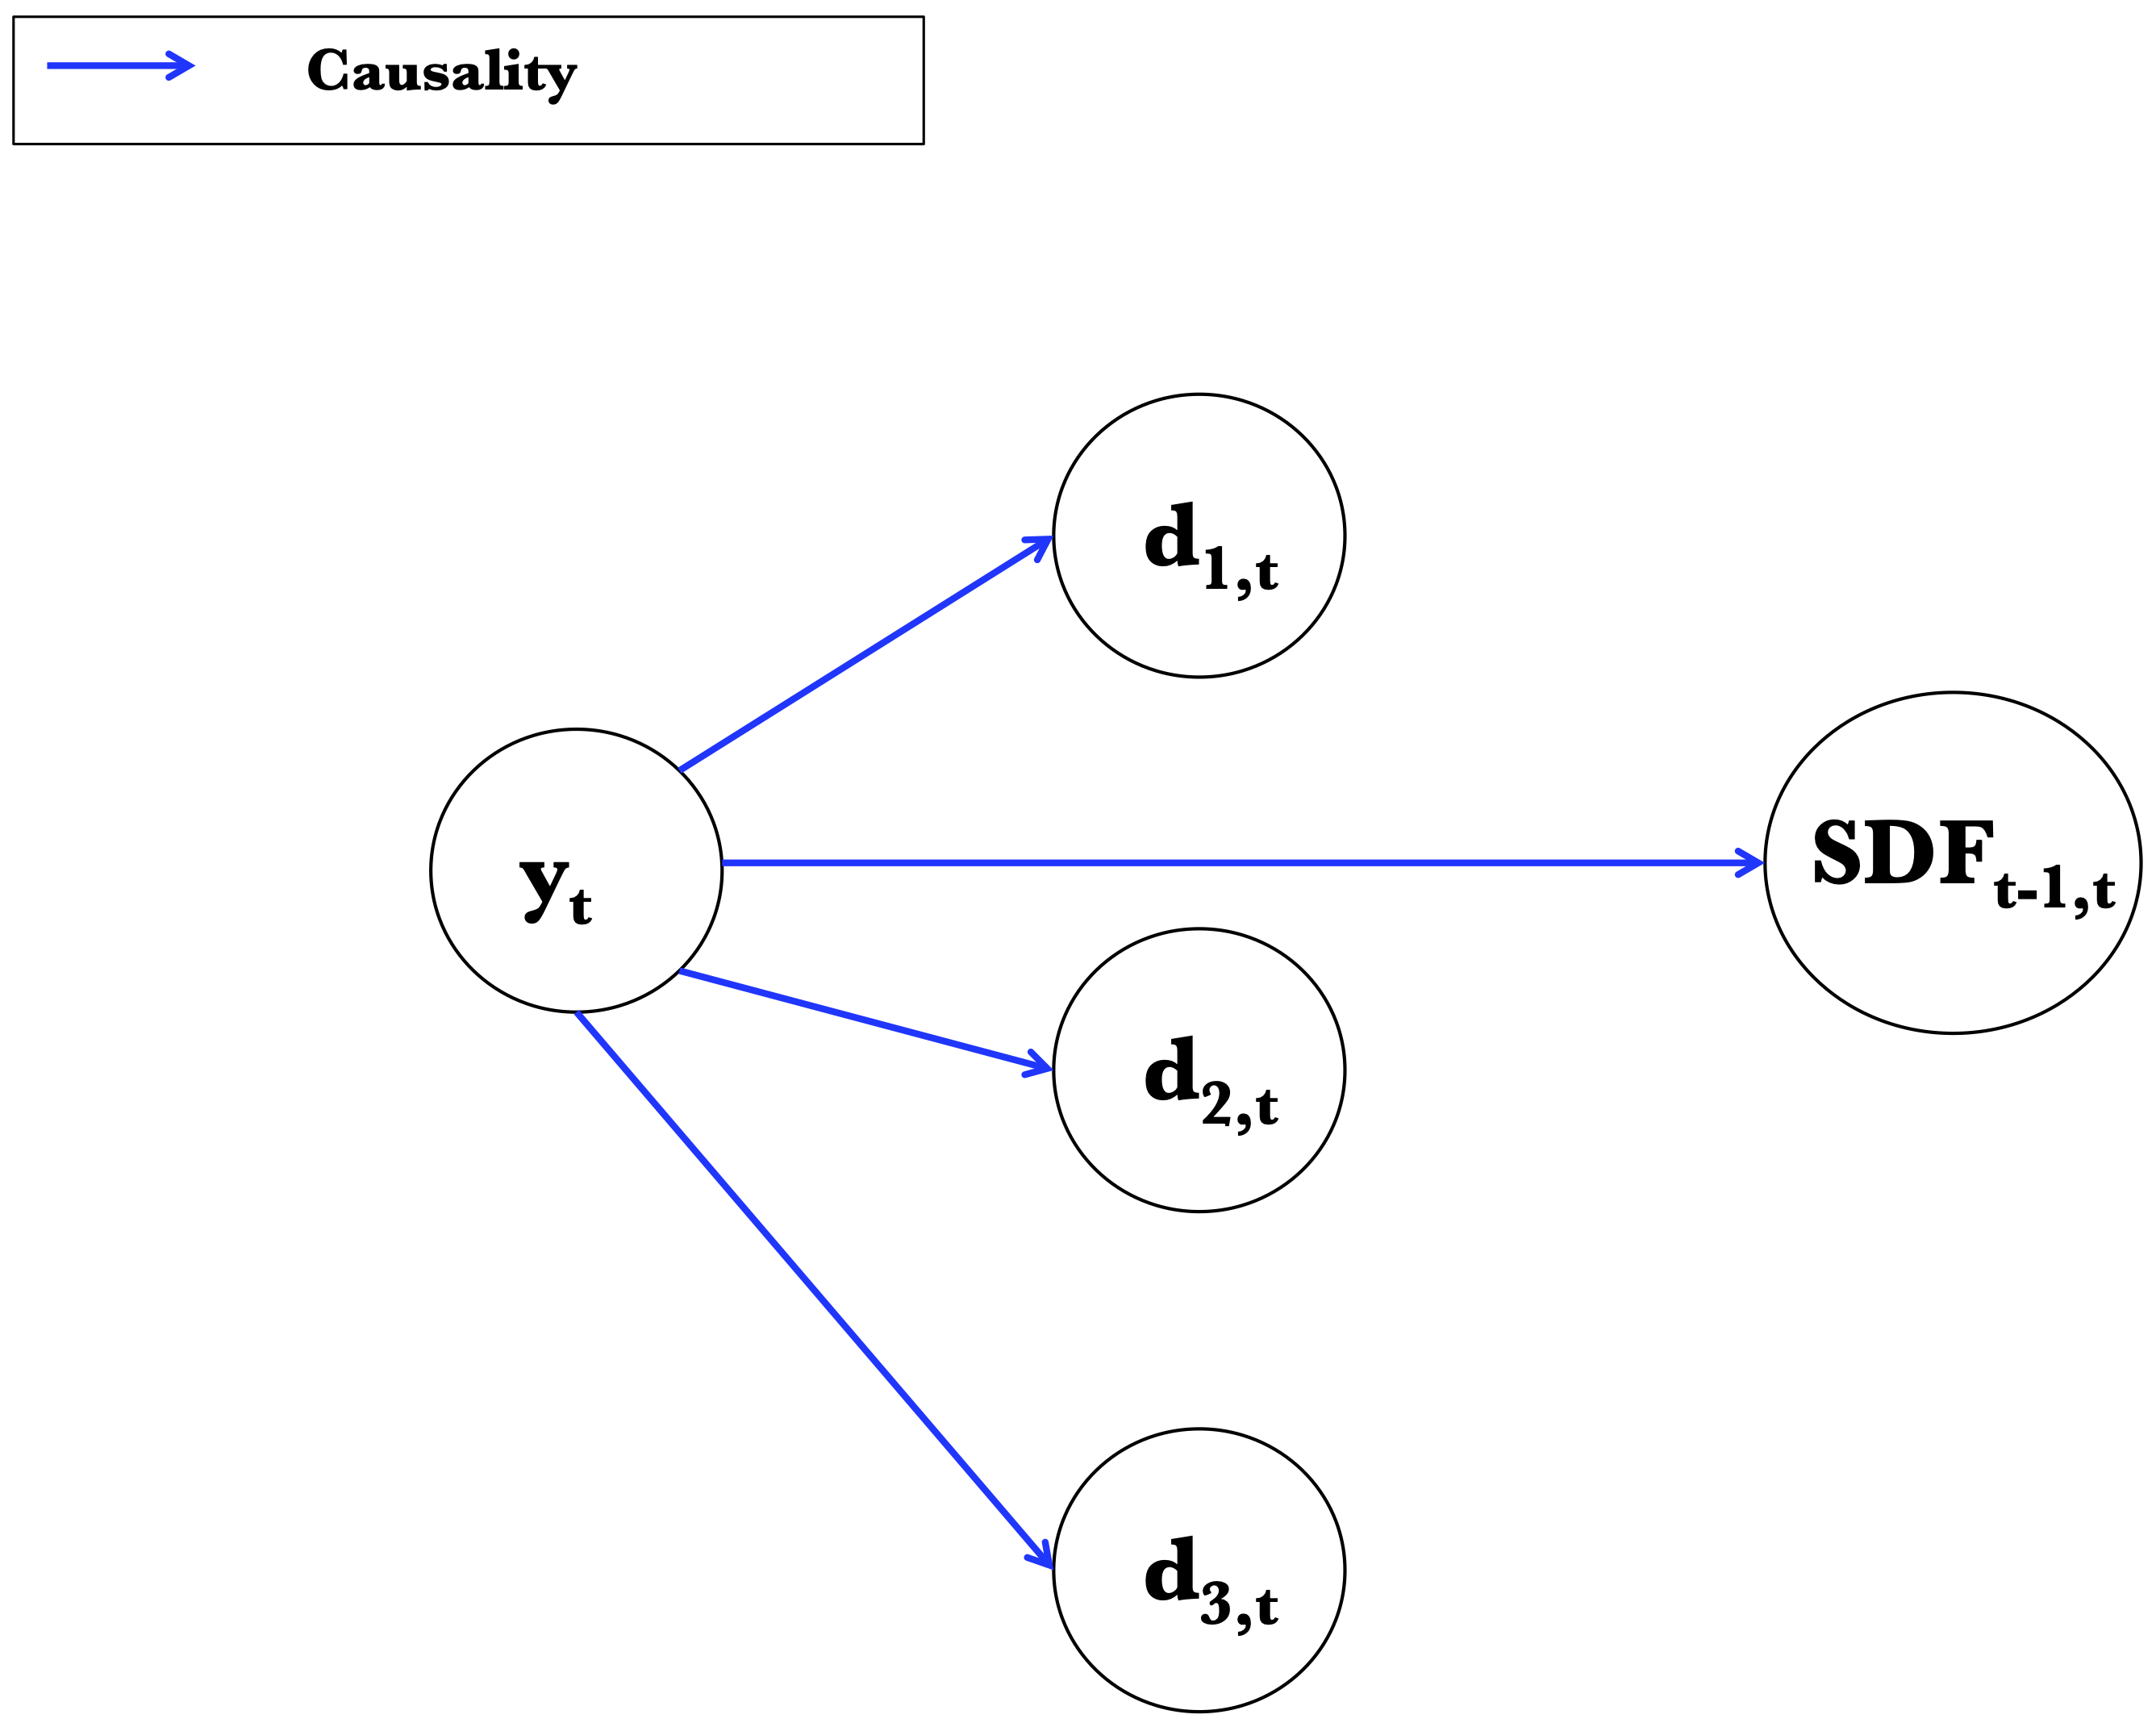
\includegraphics[width=0.8\linewidth]{figures/Schema0} 

}

\caption{Graphical representation of the causality scheme in the classical credit-risk framework.}\label{fig:classical}
\end{figure}

\begin{proposition}[Risk-neutral exogeneity of factors]
\protect\hypertarget{prp:exogdunderQ}{}\label{prp:exogdunderQ}Under Hypotheses \ref{hyp:A1} and \ref{hyp:A3}, we have:
\[
f^{\mathbb{Q}}(y_t|w_{t-1}) = f^{\mathbb{Q}}(y_t|y_{t-1}),
\]
that is, \(\{d_t\}\) does not Granger-cause \(\{y_t\}\) under the risk-neutral measure.
\end{proposition}

\begin{proof}
We have:
\begin{eqnarray}
f^{\mathbb{Q}}(y_t|w_{t-1}) &=& f(y_t|w_{t-1})\mathcal{M}_{t-1,t}\exp(i_{t-1})\\
&=& f(y_t|y_{t-1})\mathcal{M}_{t-1,t}\exp(i_{t-1}),
\end{eqnarray}
which gives the results, using that \(\mathcal{M}_{t-1,t}\) and \(\exp(i_{t-1})\) depend on \(y_{t-1}\) only (and not on \(d_t\)).
\end{proof}

To simplify, let us focus on a single entity (\(d_t \equiv d_{1,t}\)), alive on date \(t\) (\(d_t=0\)). Consider the date-\(t\) price of a bond issued by the defaultable entity. The residual maturity of this bond is denoted by \(h\), and we consider a zero recovery rate (in case of default, the payoff is zero). Using @ref\label{eq:basic}, the price of this bond writes:
\[
B^d_{t,h} = \mathbb{E}_t^{\mathbb{Q}}[\exp(-i_t-\dots-i_{t+h-1})(1-d_{t+h})].
\]

The following proposition is at the core of the \emph{classical credit-risk framework} \citep{Duffie_Singleton_1999}:

\begin{proposition}[Defaultabe zero-coupon bond pricing in the classical credit-risk framework]
\protect\hypertarget{prp:defaultBondclassical}{}\label{prp:defaultBondclassical}Under Hypotheses \ref{hyp:A1} and \ref{hyp:A3}, and with a default intensity defined---as in \eqref{eq:survival}---through:
\begin{equation}
\exp[-\lambda_t^{\mathbb{P}}]:=\mathbb{P} ( d_t=0  |  \underline{y_{t}}, d_{t-1}=0 ),
\end{equation}
we have:
\begin{equation}
\lambda_t^{\mathbb{Q}} = \lambda_t^{\mathbb{P}}\;(=\lambda_t),\label{eq:lambdaPQ}
\end{equation}
and
\begin{equation}
\boxed{B_{t,h}^d = \mathbb{E}_t^{\mathbb{Q}}\left[\exp\left(-i_t-\dots-i_{t+h-1}- \lambda_{t+1} - \dots - \lambda_{t+h}\right)\right].}\label{eq:standardPriceCredit2}
\end{equation}
which rewrites, using \(\tilde{i}_t = i_t + \lambda_{t+1}\):
\begin{equation}
B_{t,h}^d = \mathbb{E}_t^{\mathbb{Q}}\left[\exp\left(-\tilde{i}_t-\dots-\tilde{i}_{t+h-1}\right)\right],\label{eq:standardPriceCredit3}
\end{equation}
\end{proposition}

\begin{proof}
According to \eqref{eq:fQfP}:
\begin{equation}
f^{\mathbb{Q}}(d_t,y_t|d_{t-1},y_{t-1}) = \exp(i_{t-1})\mathcal{M}_{t-1,t} f^{\mathbb{P}}(d_t,y_t|d_{t-1},y_{t-1}).\label{eq:aaq1}
\end{equation}
Using Hypothesis \ref{hyp:A3}, we obtain, by integrating both sides w.r.t. \(d_t\):
\begin{eqnarray}
f^{\mathbb{Q}}(y_t|d_{t-1},y_{t-1}) &=& \exp(i_{t-1})\mathcal{M}_{t-1,t} f^{\mathbb{P}}(y_t|d_{t-1},y_{t-1})\nonumber\\
&=& \exp(i_{t-1})\mathcal{M}_{t-1,t} \underbrace{f^{\mathbb{P}}(y_t|y_{t-1})}_{\mbox{by hypothesis}}. \label{eq:aaq2}
\end{eqnarray}
By Bayes, we have:
\[
f^{\mathbb{Q}}(d_t|d_{t-1},y_t,y_{t-1}) = \frac{f^{\mathbb{Q}}(d_t,y_t|d_{t-1},y_{t-1})}{f^{\mathbb{Q}}(y_t|d_{t-1},y_{t-1})}.
\]
Using \eqref{eq:aaq1} (numerator) and \eqref{eq:aaq2} (denominator), we get:
\begin{eqnarray*}
&& f^{\mathbb{Q}}(d_t|d_{t-1},y_t,y_{t-1}) = f^{\mathbb{P}}(d_t|d_{t-1},y_t,y_{t-1}),
\end{eqnarray*}
which gives \eqref{eq:lambdaPQ}.

Conditioning w.r.t. \(\underline{y_{t+h}}\), the bond price is given by:
\begin{eqnarray*}
&& \mathbb{E}_t^{\mathbb{Q}}[\mathbb{E}_t^{\mathbb{Q}}\{\exp(-i_t-\dots-i_{t+h-1})(1-d_{t+h})|\underline{y_{t+h}}\}]\\
&=& \mathbb{E}_t^{\mathbb{Q}}[\exp(-i_t-\dots-i_{t+h-1})\mathbb{E}_t^{\mathbb{Q}}\{(1-d_{t+h})|\underline{y_{t+h}}\}]\\
&=& \mathbb{E}_t^{\mathbb{Q}}[\exp(-i_t-\dots-i_{t+h-1})\mathbb{Q}\{d_{t+h}=0|\underline{y_{t+h}}\}]\\
&=& \mathbb{E}_t^{\mathbb{Q}}\left[\exp(-i_t-\dots-i_{t+h-1})\prod_{j=1}^h\mathbb{Q}\{d_{t+j}=0|d_{t+j-1}=0,\underline{y_{t+h}}\}\right],
\end{eqnarray*}
Because Granger and Sims non-causalities are equivalent, and since \(d_t\) does not Granger-cause \(y_t\) under the risk-neutral measure (see Proposition \ref{prp:exogdunderQ}), we have:
\[
\mathbb{Q}\{d_{t+j}=0|d_{t+j-1}=0,\underline{y_{t+{\color{red}h}}}\} = \underbrace{\mathbb{Q}\{d_{t+j}=0|d_{t+j-1}=0,\underline{y_{t+{\color{red}j}}}\}}_{=\exp(-\lambda_{t+j}^{\mathbb{Q}})}.
\]
As a result:
\begin{equation}
B_{t,h}^d = \mathbb{E}_t^{\mathbb{Q}}\left[\exp\left(-i_t-\dots-i_{t+h-1}- \lambda_{t+1}^{\mathbb{Q}} - \dots - \lambda_{t+h}^{\mathbb{Q}}\right)\right].\label{eq:standardPriceCredit}
\end{equation}
Using \eqref{eq:lambdaPQ} in \eqref{eq:standardPriceCredit}, we obtain \eqref{eq:standardPriceCredit2}.
\end{proof}

\begin{quote}
Although \(\mathbb{P}\) and \(\mathbb{Q}\) intensities are the same functions of \(y_t\) and \(y_{t-1}\), their historical and risk-neutral dynamics are in general different since \(y_t\)'s \(\mathbb{P}\) and \(\mathbb{Q}\) dynamics are different.
\end{quote}

\begin{quote}
Eq. \eqref{eq:standardPriceCredit3} is reminiscent of \eqref{eq:stdbond}, where the risk-free short-term rate \(i_t\) is replaced by the \emph{credit-adjusted short-term rate} \(\tilde{i}_t\).
\end{quote}

Importantly, if both \(i_t\) and \(\lambda_t\) are affine in \(y_t\), where the latter is an affine process, then bond prices are easily computed by means of recursive formulas (as was the case in the context of \eqref{eq:stdbond}, see Example \ref{exm:nominalBth}.

In this case, \(B_{t,h}^d\) is exponential affine in \(y_t\), that is, it is of the form:
\begin{equation}
B_{t,h}^d = \exp({A^d_h}'y_t + B^d_h)\quad (say).\label{eq:standardPriceCredit4}
\end{equation}

The previous framework can be adapted in order to accommodate non-zero recovery rates. In this framework, the default intensity will be replaced by a \emph{pseudo}, or \emph{recovery-adjusted default intensity} denoted by \(\tilde\lambda_t\). To go further, we need to specifiy the payoff taking place upon default. There exist different modelling conventions for that; one is the so-called \emph{Recovery of Market Value (RMV)} \citep{Duffie_Singleton_1999}. Loosely speaking, under the RMV, the recovery payoff is a fraction \(\zeta \in [0,1]\), called \emph{Recovery Rate (RR)} of the price that would have prevailed, absent the default. Proposition \ref{prp:RMVclassical} makes this definition more precise and gives the bond price stemming from it.

\begin{proposition}[Bond pricing in the RMV classical framework]
\protect\hypertarget{prp:RMVclassical}{}\label{prp:RMVclassical}Under Hypotheses \ref{hyp:A1} and \ref{hyp:A3}, and if, in case of default on date \(t+i\), the recovery payment is \(\zeta \widetilde{B}_{t+i,h-i}\), with \(\zeta \in [0,1]\), then
\begin{equation}
B_{t,h}^d =  (1-d_t)\widetilde{B}_{t,h},\label{eq:BBcredit}
\end{equation}
where \(\widetilde{B}_{t,h}\) is a \emph{pseudo-price} given by:
\begin{equation}
\widetilde{B}_{t,h} = \mathbb{E}_t^{\mathbb{Q}} [\exp(-i_{t}-\tilde\lambda_{t+1}-\dots -i_{t+h-1}-\tilde\lambda_{t+h}],\label{eq:BtildeCredit}
\end{equation}
where the pseudo-intensity \(\tilde\lambda_{t}\) is defined by:
\begin{eqnarray}
\exp(-\tilde\lambda_{t+1}) &=&  \mathbb{E} [\{1 - d_{t+1} (1-\zeta)\}|\underline{y_{t+1}},d_t=0] \nonumber\\
&=&  1 - (1-\zeta) (1-\exp(-\lambda_{t+1})).\label{eq:pseudodefintens}
\end{eqnarray}
\end{proposition}

\begin{proof}
Relation \eqref{eq:BBcredit} is true for \(B_{t+h,0}^d\) since \(\widetilde{B}_{t+h,0} = 1\) and \(B_{t+h,0}^d = 1 - d_{t+h}\).
Assuming that \(B_{t+i+1, h-i-1}^d = (1 - d_{t+i+1} ) \widetilde{B}_{t+i+1,h-i-1}\) (which is valid for \(i=h-1\)), we get:
\begin{eqnarray*}
B_{t+i, h-i}^d &=& \left(1 - d_{t+i} \right)  \mathbb{E}_{t+i}^{\mathbb{Q}} \left\{ \exp(- i_{t+i})   \left[ \left(1 - d_{t+i+1} \right) \widetilde{B}_{t+i+1,h-i-1} \right. \right. \\
&& \left. \left. +  d_{t+i+1}\zeta\widetilde{B}_{t+i+1,h-i-1} \right] \right\},
\end{eqnarray*}
since, in case of no default at date \(t+i\), the value of the bond at date \(t+i+1\) is either \(\zeta B_{t+i+1, h-i-1}^d = \zeta \widetilde{B}_{t+i+1,h-i-1}\) if default happens, and \(B_{t+i+1, h-i-1}^d = \widetilde{B}_{t+i+1,h-i-1}\) otherwise. Hypotheses \ref{hyp:A1} and \ref{hyp:A3} imply that \(\widetilde{B}_{t+i+1,h-i-1}\) does not depend on \(d_{t+i+1}\) and taking first the conditional expectation given \(w_{t+i}\) and \(y_{t+i+1}\) we obtain:
\begin{equation}
\begin{array}{lll}
B_{t+i, h-i}^d &=& \left(1 - d_{t+i} \right) \mathbb{E}_{t+i}^{\mathbb{Q}} \left\{ \exp(- i_{t+i})  \widetilde{B}_{t+i+1,h-i-1} \times \right. \\
&& \quad\left. \mathbb{E}^{\mathbb{Q}} \left[ \left(1 - d_{t+i+1} \right) +  \zeta d_{t+i+1}  | y_{t+i+1}, w_{t+i} \right] \right\} .
\end{array}\label{eq:Prop21demo}
\end{equation}
Using the definition of \(\widetilde{\lambda}_{t}\) (Eq. \eqref{eq:pseudodefintens}) we get:
\begin{equation*}
\begin{array}{lll}
B_{t+i, h-i}^d &=& \left(1 - d_{t+i} \right)  \mathbb{E}_{t+i}^{\mathbb{Q}} \left\{ \exp \left( - i_{t+i} - \widetilde{\lambda}_{t+i+1} \right)  \widetilde{B}_{t+i+1,h-i-1} \right\}\\
&=& \left(1 - d_{t+i} \right)   \widetilde{B}_{t+i,h-i} .
\end{array}
\end{equation*}
Therefore it is also true for \(i=0\).
\end{proof}

Again, if \(i_t\) and \(\tilde\lambda_t\) are affine combinations of an affine process \(y_t\), then (exponential affine) bond prices are easily computed by means of recursive formulas. This is formalized below.

\begin{hypothesis}[Affine process]
\protect\hypertarget{hyp:A6}{}\label{hyp:A6}The process \(\{ y_t \}\) is affine under the \(\mathbb{Q}\) measure:
\begin{equation}
\begin{array}{lll}
\varphi^{\mathbb{Q}}_{y, t-1} (u_y) = \mathbb{E}^{\mathbb{Q}} \left[\exp( u_y ' y_t )   |   \underline{y_{t-1}} \right]
= \exp \left[ a^{\mathbb{Q}}_{y} (u_{y}) ' y_{t-1} + b^{\mathbb{Q}}_{y} (u_{y}) \right],
\end{array}\label{eq:affineyPcLT}
\end{equation}
and \(i_t\) and \(\widetilde{\lambda}_{e, t}\) are affine in \((y_t, y_{t-1})\), that is (say):
\begin{eqnarray}
i_{t} &=& \omega_0 + \omega_{1} ' y_{t} \\
\widetilde{\lambda}_{e, t} &=& \kappa_{0} + \kappa_{1}' y_t.
\end{eqnarray}
\end{hypothesis}

\begin{proposition}[Standard affine bond pricing, under RMV convention]
\protect\hypertarget{prp:standardCreditFormula}{}\label{prp:standardCreditFormula}Under the Assumptions of Proposition \ref{prp:RMVclassical} and under Hypothesis \ref{hyp:A6}, we have, for \(h \ge 1\):
\begin{equation}
B_{t,h}^d = \left(1 - d_{t} \right)\exp(- h[\omega_0 + \kappa_{0}] - \omega_{1} ' y_{t} + A_h'y_t + B_h),\label{eq:standardAffineCredit}
\end{equation}
where \(A_h\) and \(B_h\) are given by the following recursive equations:
\begin{equation}
\left\{
\begin{array}{ccl}
A_{h} &=& a(u_{h} + A_{h-1}), \\
B_{h} &=& b(u_{h} + A_{h-1}) + B_{h-1}, \\
A_{0} &=& 0,\quad  B_{0} = 0,
\end{array}
\right.\label{eq:auxRecursiveStandardCredit}
\end{equation}
with \(u_1 = -\kappa_{1}\) and \(u_i = -(\kappa_{1} + \omega_{1})\) for \(i>1\).
\end{proposition}

\begin{proof}
The results directly follows from Proposition \ref{prp:RMVclassical}.
\end{proof}

What precedes has been estiablished under the assumption that the state vector \(w_t\) comprises a single defaultable entity (\(E=1\)). What about when different entities are considered (\(E = 2\))? We can demonstrate that similar pricing formulas are obtained under the assumption of no-contagion (Hypothesis \ref{hyp:A2}):

\begin{hypothesis}[no contagion]
\protect\hypertarget{hyp:A2}{}\label{hyp:A2}There is no instantaneous or lagged contagion between entities, i.e.:
\begin{equation*}
p ( d_t  |  y_t, w_{t-1} ) = p_1 ( d_{1, t}  |  y_t, y_{t-1}, d_{1, t-1})   \times   p_2 ( d_{2, t}  |  y_t, y_{t-1}, d_{2, t-1}) .
\end{equation*}
\end{hypothesis}

If Hypothesis \ref{hyp:A2} is not satisfied, for instance, if we have contagion effect from \(e = 1\) towards \(e = 2\):
\begin{eqnarray*}
p(d_t|y_t, w_{t-1} ) &=& p_1 ( d_{1, t}  |  y_t, y_{t-1}, d_{1, t-1}) \times \\
&&  p_2 ( d_{2, t}  |  y_t, y_{t-1}, \color{blue}{d_{1, t}}, \color{blue}{d_{1, t-1}}, d_{2, t-1}),
\end{eqnarray*}
then:

\begin{enumerate}
\def\labelenumi{\arabic{enumi}.}
\tightlist
\item
  Proposition \ref{prp:RMVclassical} is still valid for both entities;
\item
  In an affine framework, the computation of \(\widetilde{B}^{(1)}_{t,h}\) (and \(B^{(1)}_{t,h}\)) is straightforward;
\item
  but formulas for \(\widetilde{B}^{(2)}_{t,h}\) and \(B^{(2)}_{t,h}\) are not explicit anymore even if \(\widetilde{\lambda}_{2, t}\) is affine in \((y_t, y_{t-1}, d_{1, t}, d_{1, t-1})\).
\end{enumerate}

\begin{proposition}[Absence of contagion]
\protect\hypertarget{prp:defBondAffine}{}\label{prp:defBondAffine}Under Hypotheses \ref{hyp:A4}, \ref{hyp:A1}, \ref{hyp:A3} and \ref{hyp:A2}, the risk-neutral (\(\mathbb{Q}\)) dynamics is such that:
\[
f^{\mathbb{Q}} ( y_t  |  w_{t-1}) = f^{\mathbb{Q}} ( y_t  |  y_{t-1}) \propto \mathcal{M}_{t-1, t}( y_t, y_{t-1}) f (y_t  |  y_{t-1})
\]
(\emph{exogeneity of \(y_t\) preserved under \(\mathbb{Q}\)}) and

\[
p_t^{\mathbb{Q}} ( d_{t}  |  y_t, w_{t-1} ) = p_1 ( d_{1, t}  |  y_t, y_{t-1}, d_{1, t-1} )   \times   p_2 ( d_{2, t}  |  y_t, y_{t-1}, d_{2, t-1}),
\]
(\emph{absence of contagion preserved under \(\mathbb{Q}\)}).

Denoting by \(\lambda^{\mathbb{Q}}_e \left( y_t, y_{t-1} \right) \equiv - \log \left[ p_e^{\mathbb{Q}} ( 0 | y_t, y_{t-1}, 0 ) \right]\) the \emph{risk-neutral default intensity} of entity
\(e\), it comes that:
\[
\lambda^{\mathbb{Q}}_e \left( y_t, y_{t-1} \right) = \lambda_e \left( y_t, y_{t-1} \right)
\]
(\emph{default intensities are the same under \(\mathbb{P}\) and \(\mathbb{Q}\)}).
\end{proposition}

\begin{proof}
The \(\mathbb{Q}\) conditional density of \(w_t\) given \(w_{t-1}\), namely \(f^{\mathbb{Q}} (y_t | w_{t-1}) p^{\mathbb{Q}} ( d_t | y_t, w_{t-1} )\), is proportional to \(\mathcal{M}_{t-1, t}( w_t, w_{t-1}) f (y_t | w_{t-1}) p ( d_t | y_t, w_{t-1} )\), and thus proportional to \(\mathcal{M}_{t-1, t}( y_t, y_{t-1}) f (y_t | y_{t-1}) p_1 ( d_{1, t} | y_t, y_{t-1}, d_{1, t-1}) p_2 ( d_{2, t} | y_t, y_{t-1}, d_{2, t-1})\). The result follows immediately.
\end{proof}

\hypertarget{CreditIlliq}{%
\section{Pricing illiquid bonds}\label{CreditIlliq}}

This subsection shows that a similar approach can be used to price illiquid assets. The idea consists in replacing the Loss Given Default (\(LGD = 1-RR^{(e)}\)) by a Loss Given Liquidity Shock (\(1-\theta_\ell^{(e)}\)). A structural interpretation of this approach is provided by \citet{Ericsson_Renault_2006} (see Example \ref{exm:illiqLGD}).

Let us introduce a novel binary variable: \(\ell_t\), that represents a \emph{liquidity shocks}. When a bondholder is hit by the liquidity shock, she needs to liquidate her portfolio (reflecting cash constraints or needs to rebalance portfolio). But in such distressed conditions, she will sell her bonds at a discount (and will therefore face losses, akin to credit losses). Formally: \(\ell_{t}=1\) when the bondholder is hit, and \(\ell_{t}=0\) otherwise.

The \emph{liquidity-shock intensity} \(\lambda_\ell(y_t)\)---that defines the probability of occurence of liquidity shocks---is defined through:
\[
\underbrace{1- \exp[-\lambda_\ell(y_t)]}_{\approx \lambda_\ell(y_t)\mbox{ if small}} = \mathbb{P}(\ell_t = 1|\underline{w_{t-1}},y_t).
\]
The binary variable \(\ell_t\) is assumed not to Granger-cause \(y_t\) (as in Hypothesis \ref{hyp:A1}) and not to be priced (as in Hypothesis \ref{hyp:A3}). As in Proposition \ref{prp:defaultBondclassical}---and more precisely \eqref{eq:lambdaPQ}---this implies that
\[
\lambda_\ell^{\mathbb{Q}}(y_t) = \lambda_\ell(y_t),
\]
where
\[
1- \exp[-\lambda^{\mathbb{Q}}_\ell(y_t)] = \mathbb{Q}(\ell_t = 1|\underline{w_{t-1}},y_t).
\]

Upon the arrival of the liquidity shock (\(\ell_{t}=1\)), the investor has to exit by selling her bond holdings. She is then limited in the number of traders she can call and, as a result, get only a fraction (\(\theta_\ell^{(e)}\), say) of the price she would get in normal-liquidity times, i.e., when \(\ell_{t}=0\) (see the structural interpretation in Example \ref{exm:illiqLGD}).

In that context, following the approach used in Proposition \ref{prp:RMVclassical}, one can define a \emph{pseudo-illiquidity intensity} as follows---mimicking \eqref{eq:pseudodefintens}:
\begin{eqnarray}
\widetilde{\lambda}_{e,\ell, t} \left( y_t, y_{t-1} \right) &=& - \log \left\{ \exp \Big[ -
\lambda_{e,\ell} \left( y_t\right) \Big] \right. + \label{eq:pseudoilliqintensity}\\
&& \left. \Big( 1 - \exp \Big[ - \lambda_{e,\ell} \left( y_t \right) \Big]
\Big) \theta_\ell^{(e)}  \right\}. \nonumber
\end{eqnarray}

Still consiering credit risk (on top of liquidity risk), we then have the following payoff on date \(t\) (assuming no default on date \(t-1\)):
\begin{equation}
\widetilde{B}^{(e)}_{t,h} = \mathbb{E}^{\mathbb{Q}}_t \left\{ \exp \left[ - \sum_{i=1}^{h} \left( i_{t+i-1} + \widetilde{\lambda}_{e,c, t+i} + \widetilde{\lambda}_{e,\ell, t+i} \right) \right] \right\}.\label{eq:pseudopriceilliq}
\end{equation}

\begin{example}[Structural interpretation of the illiquidity intensity]
\protect\hypertarget{exm:illiqLGD}{}\label{exm:illiqLGD}This structural interpretation of the illiquidity intensity is due to \citet{Ericsson_Renault_2006}.

When hit by a liquidity shock, a bondholder has to liquidate her bond in a small amount of time (between \(t\) and \(t+\varepsilon\), with \(\varepsilon \ll 1\)). She collects offers on the market; each offer is a random fraction \(\omega_{i}\) (\(i\in\{1,\ldots,\kappa\}\)) of \(\widetilde{B}^{(w)}_{t,h}\) (see Eq. \eqref{eq:pseudopriceilliq}), where the \(\omega_{i}\)'s are uniformly distributed in \([0,1]\).

At \(t+\varepsilon\), the bond is sold to the trader that has offered the highest price. Formally, when \(\ell_{t}=1\), the selling price is:
\[
\left(\max_{i\in\{1,\ldots,\kappa\}}\omega_{i}\right)\tilde{P}_{t,h}^{(e)}.
\]
Conditional on \(\kappa\), the expectation of \(\max_{i}(\omega_{i})\) is \(\kappa/(\kappa+1)\). (Because the \(\omega_{i}\) are i.i.d., the c.d.f. of \(\max(\omega_{1},\ldots,\omega_{\kappa})\) is \(x\mapsto F(x)^{\kappa}\), where \(F\) is the c.d.f. of \(\omega_{i}\).)
Hence, \(\theta_\ell^{(e)}\)---the unconditional expectation of \(\max_{i}(\omega_{i})\)---is given by:
\begin{eqnarray*}
\sum_{k=1}^{\infty}\frac{e^{-\varepsilon\gamma^{(e)}}k}{k+1}\frac{\left(\varepsilon\gamma^{(e)}\right)^{k}}{k!} & = & \left[\left(1-e^{-\varepsilon\gamma^{(e)}}\right)\frac{\varepsilon\gamma^{(e)}-1}{\varepsilon\gamma^{(e)}}+e^{-\varepsilon\gamma^{(e)}}\right]\\
& = & g(\varepsilon\gamma^{(e)})\qquad\mbox{(say).}
\end{eqnarray*}
Function \(g\) is increasing and valued in \([0,1]\). In addition \(\lim_{x\rightarrow\infty}g(x)\rightarrow1\).
\end{example}

\begin{example}[Euro area sovereign credit spreads]
\protect\hypertarget{exm:SovereignSpreads}{}\label{exm:SovereignSpreads}

\citet{Monfort_Renne_NER2011} and \citet{Monfort_Renne_2014} propose credit/liquidity decompositions of euro-area sovereign spreads. They emply different estimation approaches: \citet{Kim_1994}'s filter for MR2014, and Kitagawa-Hamilton filter for \citet{Monfort_Renne_NER2011} (see Subsection \ref{EstimationRS}).

In both papers, the \(y_t\) part of the state vector \(w_t\) is of the form \(y_t = (x_t',z_t')'\); it follows a Regime-Switching Gaussian VAR (see Example \ref{exm:GRSVAR}). The time-homogenous Markov chain \(z_t\) tracks the \emph{crisis status} (crisis versus normal times).

The total intensity is of the form:
\[
\widetilde{\lambda}_{e,t} = \underbrace{\alpha_{e,c}'z_t + \beta_{e,c}'y_t}_{\mbox{credit intensity $\widetilde{\lambda}_{e,c,t}$}} + \underbrace{\alpha_{e,\ell}'z_t + \beta_{e,\ell}'y_t.}_{\mbox{liquidity intensity $\widetilde{\lambda}_{e,\ell,t}$}}
\]
In both papers, the identification of credit versus liquidity components is based on:
\[
\mbox{KfW-Bund spreads} =  \mbox{liquidity spreads}.
\]
KfW (\emph{Kreditanstalt für Wiederaufbau}) is a German agency whose bonds are guaranteed by the Federal Republic of Germany. Therefore, they benefit from the same credit quality than their sovereign counterparts---the Bunds---but are less liquid; accordingly, the KfW-Bund spread should beessentially liquidity-driven.

In \citet{Monfort_Renne_2014}, we have
\[
\widetilde{\lambda}_{e,t} = \underbrace{x_{e,t}}_{=\widetilde{\lambda}_{e,c,t}} + \underbrace{(1-\theta^{(e)}_\ell)x_{E+1,t}}_{=\widetilde{\lambda}_{e,\ell,t}},
\]
hence \(x_t\) of dimension \(E+1 = 12\) (11 countries are involved).

There are 9 Markovian regimes: \(z_t = z_{c,t} \otimes z_{\ell,t}\), where \(z_{i,t}\) (\(i \in \{c,\ell\}\)) is 3-dimensional:

\begin{itemize}
\tightlist
\item
  \(z_{i,t}=[1,0,0]'\): low stress,
\item
  \(z_{i,t}=[0,1,0]'\): medium stress,
\item
  \(z_{i,t}=[0,0,1]'\): high stress.
\item
  \(z_{c,t}\) and \(z_{\ell,t}\) are not independent: for instance, the probability to transit from the low-credit-stress regime to the medium/high-credit-stress regimes depends on the liquidity-stress regime.
\end{itemize}

For each intensity \(x_{i,t}\) (simulation below XXX):
\[
x_{i,t} = \mu_i'z_t + \phi x_{i,t-1} + \sigma_i \varepsilon_{i,t},
\]
with \(\varepsilon_{t} \sim i.i.d. \mathcal{N}(0,\Sigma)\), where \(\Sigma\) is diagonal, and \(\mu_{i,1} < \mu_{i,2} < \mu_{i,3}\).
The Markov chain \(z_t\) is the only source of correlation across the \(x_{i,t}\)'s.

Figure \ref{fig:MRintensity} shows a simulation of such a process, with:
\[
\mu=\left[\begin{array}{c}
0.01 \\ 0.03 \\ 0.10\end{array}\right],\quad \phi=.8 ,\quad P=\left[\begin{array}{ccc}
0.98 & 0.02 & 0\\
0.05 & 0.90 & 0.05\\
0 & 0.20 & 0.80
\end{array}\right],\quad \sigma = 0.002.
\]

The SDF exponential affine in \((z_t',x_t')'\). We have the same type of dynamics under \(\mathbb{Q}\) (with risk-asjusted parameters, in particular risk-adjusted transition probabilities).

\begin{figure}
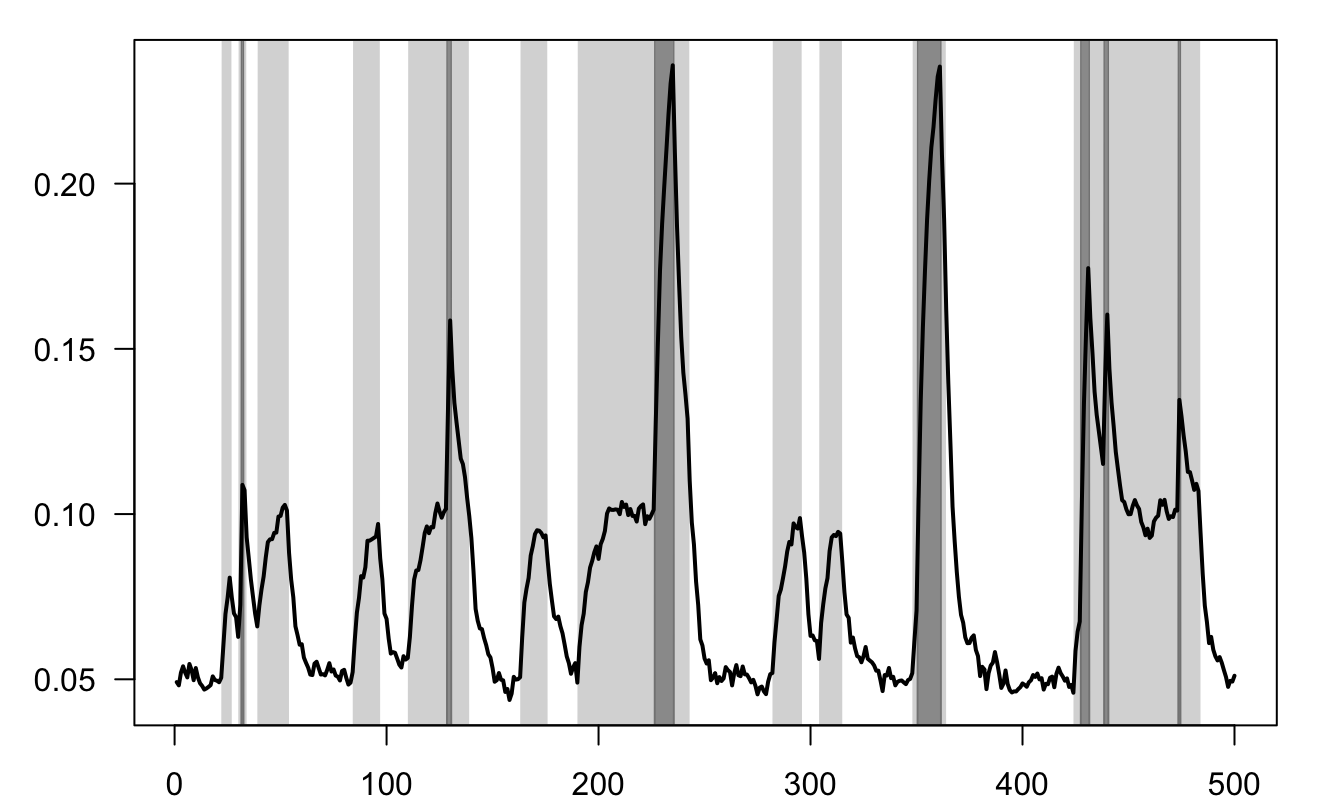
\includegraphics[width=0.95\linewidth]{TSM_files/figure-latex/MRintensity-1} \caption{Simulation of an process following $x_{t} = \mu'z_t + \phi x_{t-1} + \sigma \varepsilon_{t}$, where $z_t$ follows a three-state time-homogenous Markov process. See the text for the exact parameterization. The light-grey shaded area corresponds to the second regime ($z_t = [0,1,0]'$); the dark-grey shaded area corresponds to the third regime ($z_t = [0,0,1]'$)}\label{fig:MRintensity}
\end{figure}

\end{example}

\begin{example}[IBOR-OIS spreads]
\protect\hypertarget{exm:IBOROIS}{}\label{exm:IBOROIS}

\citet{DUBECQ201629} decompose the EURIBOR versus Overnight Index Swap (OIS) spreads into a credit and a liquidity component. (See Subsection \ref{Swaps} for the definition of a swap contract.)

From the point of view of bank \(j\), the EURIBOR rate is the rate of an unsecured loan to one bank (\(e\), say) of the panel. Assume that the panel of the \(N\) constituting the EURIBOR are homogenous. We have:
\begin{equation}
R^{IBOR}_{t,h} = - \frac{1}{h} \log \mathbb{E}^{\mathbb{Q}}_t \left\{ \exp \left[ - \sum_{i=1}^{h} \left( i_{t+i-1} + \widetilde{\lambda}_{e,c, t+i} + \widetilde{\lambda}_{j,\ell, t+i} \right) \right] \right\}.\label{eq:EURIBOR}
\end{equation}
Note that the liquidity intensity refers to the lending bank (\(j\)) and the default intensity relates to the borrowing bank (\(e\)).

By constrast, the Overnight-Index Swap (OIS) rate satisfies:\footnote{The OIS is an interest-rate swap where the floating rate is an overnight-rate reference (EONIA in the euro area). At maturity, the payoff received by the fixed-rate payer is the difference between: (a) the notional (\(W\), say) inflated with the date-\(t\) OIS (fixed) rate (i.e.~\(W\exp\{h i_{t,h}^{OIS}\}\)) and (b) the same notional capitalized with the realized short-term rates (i.e.~\(W\exp\{i_{t} + \ldots + i_{t+h-1}\}\)).}
\begin{equation}
R^{OIS}_{t,h} = - \frac{1}{h} \log \mathbb{E}^{\mathbb{Q}}_t \left\{ \exp \left( - \sum_{i=1}^{h}  i_{t+i-1} \right) \right\}.\label{eq:OIS}
\end{equation}

Assuming that \(i_t\), the short-term risk-free rate (i.e., the reference rate of the OIS, EONIA here) is independent from the intensities and under the homogeneity assumption, we obtain:\footnote{It is assumed here that the overnight interbank market preserves the lending bank from (i) liquidity and (ii) credit risk. The rationale behind that is twofold: (a) By rolling its cash on the overnight market (at the EONIA rate), a bank is not exposed to the risk of having to liquidate longer-term investments upon the realization of the liquidity shock; (b) while the EONIA is an unsecured-transaction rate, the extremely-short maturity of these transactions substantially reduces the credit-risk exposure of the lending bank.}
\[
R^{IBOR}_{t,h} - R^{OIS}_{t,h} = - \frac{1}{h} \log \mathbb{E}^{\mathbb{Q}}_t \left\{ \exp \left[ - \sum_{i=1}^{h} \left( \widetilde{\lambda}_{c, t+i} + \widetilde{\lambda}_{\ell, t+i} \right) \right] \right\}.
\]

\citet{DUBECQ201629} employ a quadratic specification for \(\widetilde{\lambda}_{c, t}\) and \(\widetilde{\lambda}_{\ell, t}\):
\[
\widetilde{\lambda}_{c, t} = x_{c,t}^2 \quad \mbox{and} \quad  \widetilde{\lambda}_{\ell, t} = x_{\ell,t}^2,
\]
where \(X_t = (x_{c,t},x_{\ell,t})'\) follows a Gaussian VAR(1) process. (This is the quandratic Gaussian framework presented in Example \ref{exm:QGVAR1}.)

The state vector \(X_t\) is latent. The estimation involves the Quadratic Kalman Filter \citep{Monfort_Renne_Roussellet_2015}. The measurement equations include equations stating that observed proxies of credit and liquidity risks relate to quadratic functions of \(x_{c,t}\) and \(x_{\ell,t}\), respectively.

\begin{figure}

{\centering 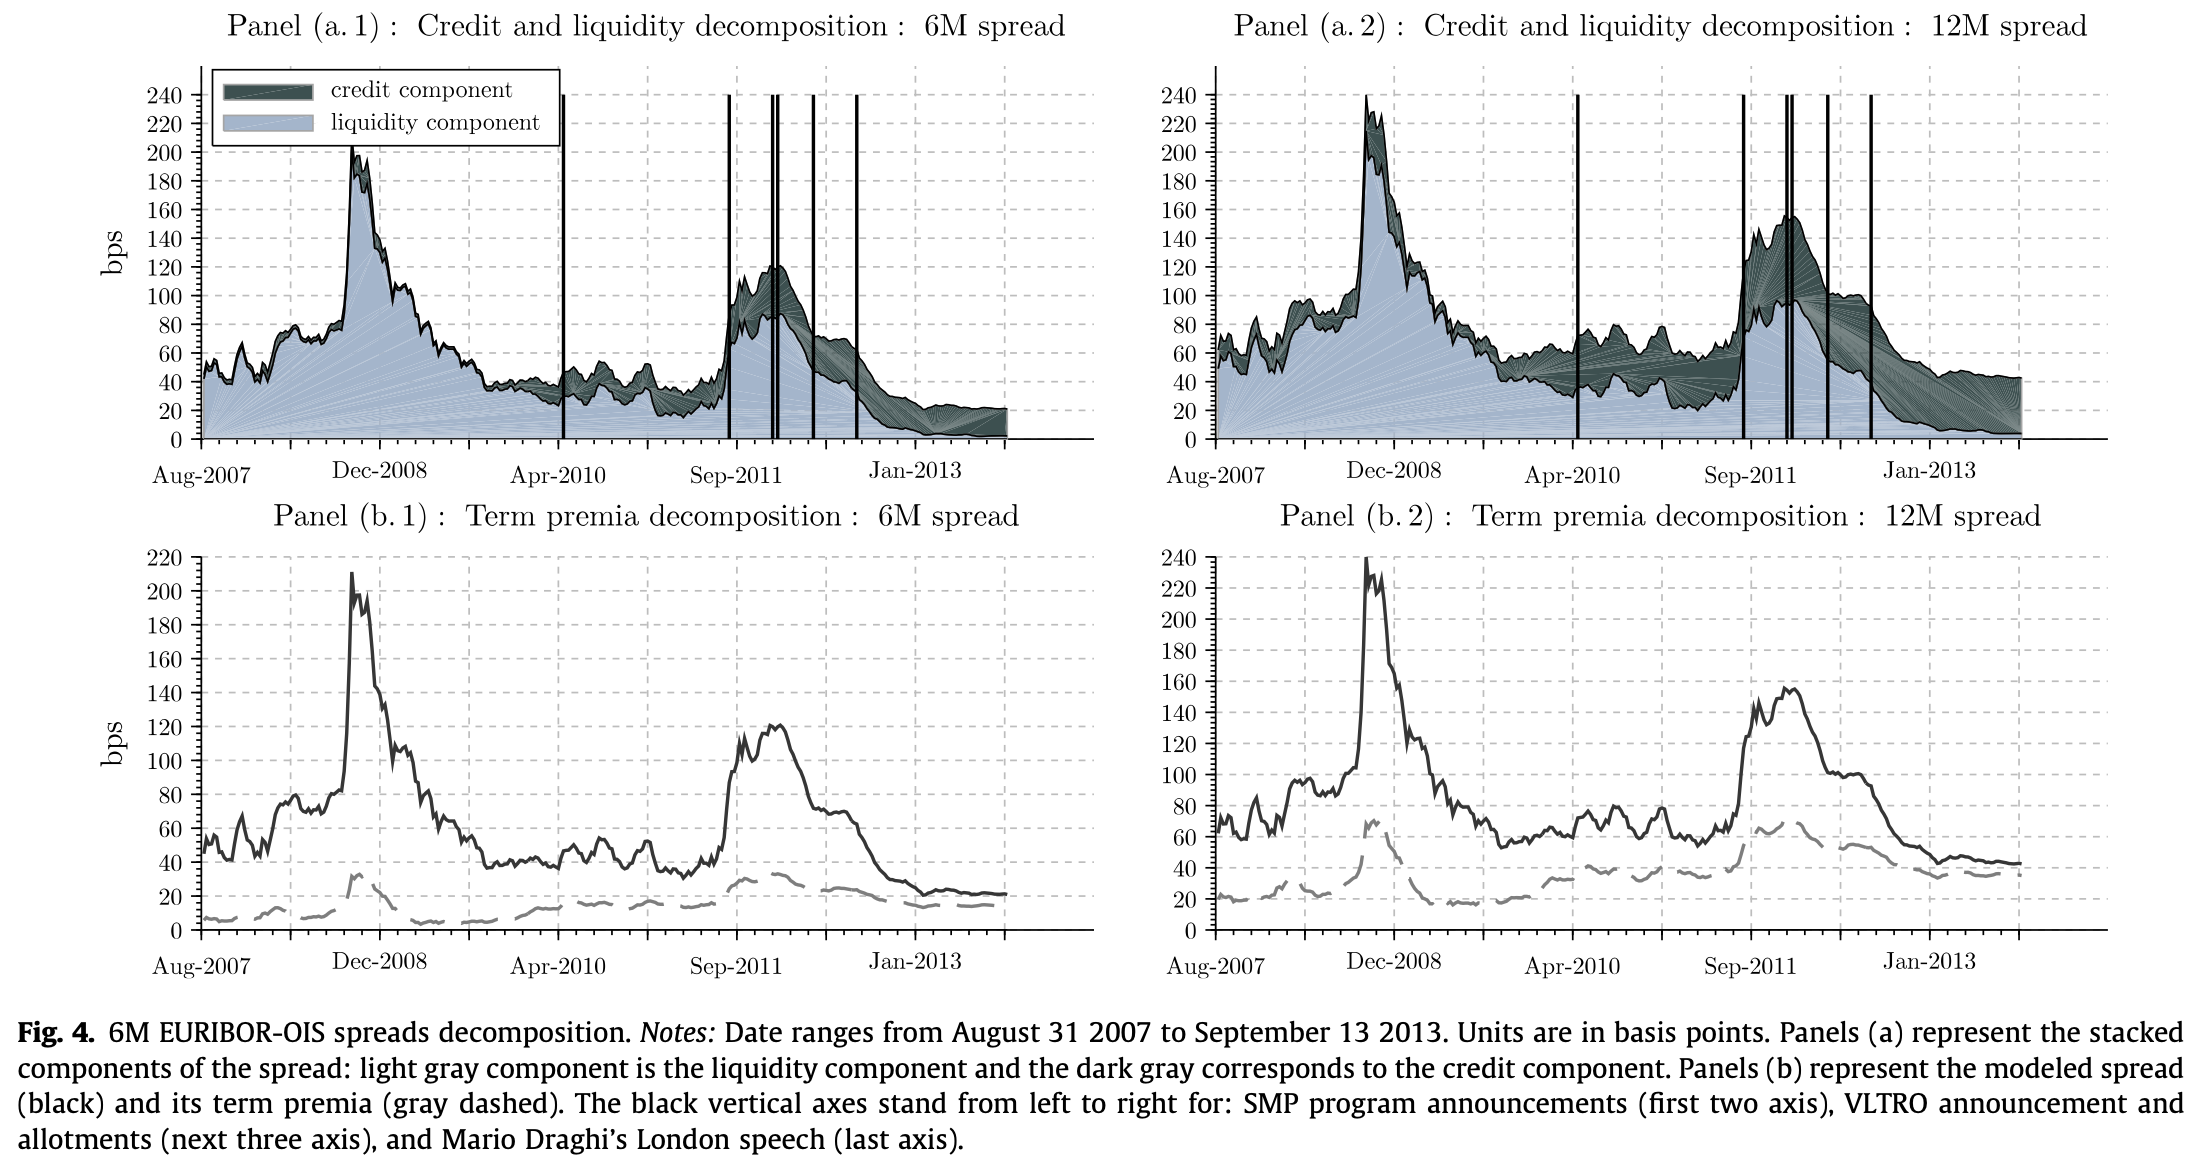
\includegraphics[width=0.95\linewidth]{figures/IBOROIS} 

}

\caption{Source: Dubecq et al. (2016).}\label{fig:IBOROIS}
\end{figure}

\end{example}

\hypertarget{Creditrelaxing}{%
\section{Relaxing the classical framework assumptions}\label{Creditrelaxing}}

Formula \eqref{eq:standardAffineCredit} and its tractability is a key feature of numerous credit-risk term-structure models, e.g., \citet{Duffie_Singleton_2003}, \citet{Pan_Singleton_2008}, and \citet{Longstaff_Pan_Pedersen_Singleton_2011} among many others. This formula is valid under Assumptions \ref{hyp:A1} of non-systemic entities, also called \emph{no-jump condition}, \ref{hyp:A3} of unpriced credit risk events, and \ref{hyp:A2} absence of contagion. These hypotheses define what we have called the \emph{classical credit-risk models}. We lose the high degree of tractability of Formula \eqref{eq:standardAffineCredit} when some of the previous assumptions are relaxed:

\begin{itemize}
\item
  If \(f (y_t | w_{t-1}) = f (y_t | y_{t-1} , d_{1, t-1})\) (entity \(e = 1\) is \emph{systemic}) then:

  \begin{enumerate}
  \def\labelenumi{\alph{enumi}.}
  \tightlist
  \item
    The pseudo-price \(\widetilde{B}^{(e)}_{t,h}\) now depends on \(y_t\) and \(d_{1, t}\);
  \item
    Eq. \eqref{eq:standardPriceCredit2} is valid for entity \(e = 2\) only;
  \item
    The computation of \(\widetilde{B}^{(2)}_{t,h}\) is not straightforward: \(\{ y_t \}\)
    is not autonomous and the autonomous process \(\{ y_t, d_{1,t} \}\) is not affine.
  \end{enumerate}
\item
  If there is a contagion effect from \(e = 1\) towards \(e = 2\), i.e., if
  \begin{eqnarray*}
  p ( d_t  |  y_t, w_{t-1} ) &=& p_1 ( d_{1, t}  |  y_t, y_{t-1}, d_{1, t-1}) \\
  &&  p_2 ( d_{2, t}  |  y_t, y_{t-1}, d_{1, t}, d_{1, t-1}, d_{2, t-1}),
  \end{eqnarray*}
  then:

  \begin{enumerate}
  \def\labelenumi{\alph{enumi}.}
  \tightlist
  \item
    Eq. \eqref{eq:standardPriceCredit2} is still valid for both entities;
  \item
    In an affine framework, the computation of \(\widetilde{B}^{(1)}_{t, h}\) (and \(B^{(1)}_{t,h}\)) is straightforward; but formulas for \(\widetilde{B}^{(2)}_{t,h}\) and \(B^{(2)}_{t,h}\) are not explicit anymore even if \(\widetilde{\lambda}_{2, t}\) is affine in \((y_t, y_{t-1}, d_{1, t}, d_{1, t-1})\).
  \end{enumerate}
\item
  If the default event of the first entity only (\(d_{1,t}\)) is a source of risk that is priced: \(\mathcal{M}_{t-1, t}( w_t, w_{t-1}) = \mathcal{M}_{t-1, t}( y_t, y_{t-1}, d_{1, t}, d_{1, t-1})\), then

  \begin{enumerate}
  \def\labelenumi{\alph{enumi}.}
  \tightlist
  \item
    \(\lambda^{\mathbb{Q}}_{1, t} \neq \lambda_{1, t}\) and \(\lambda^{\mathbb{Q}}_{2, t} = \lambda_{2, t}\);
  \item
    the exogeneity of \(\{ y_t \}\) is no longer preserved under \(\mathbb{Q}\);
  \item
    Eq. \eqref{eq:standardPriceCredit2} is no longer valid for entity \(e = 1\). It remains valid for \(e=2\) but the computation of \(\widetilde{B}^{(2)}_{t,h}\) is not straightforward: even if \(y_t\) is \(\mathbb{P}\)-autonomous, this is not true under \(\mathbb{Q}\).
  \end{enumerate}
\end{itemize}

\hypertarget{CreditGeneral}{%
\subsection{General affine credit-risk framework}\label{CreditGeneral}}

Exploiting Vector Auto-Regressive Gamma (VARG) processes, \citet{Monfort_Pegoraro_Renne_Roussellet_2021} propose a general affine credit-risk pricing model jointly allowing for:

\begin{enumerate}
\def\labelenumi{\arabic{enumi}.}
\tightlist
\item
  \emph{systemic entities} (breaking down the no-jump condition; see \citet{CollinDufresne_Goldstein_Hugonnier_2004});
\item
  \emph{contagion effects between entities} (economic/financial linkages; see \citet{AITSAHALIA2014151});
\item
  \emph{pricing of credit events} (credit spread puzzle; see \citet{Gourieroux_Monfort_Renne_2014});
\item
  and \emph{stochastic recovery rates (RR)} \citep{Altman_Brady_Resti_Sironi_2005}.
\end{enumerate}

In this general framework, the state vector \(w_t\) is of the form \([y_t',\delta_t']'\), where \(\delta_t\) is a \(E\)-dimensional vector of \emph{credit-event variables} (see Hypothesis \ref{hyp:H1}).

\begin{figure}

{\centering \includegraphics[width=0.8\linewidth]{figures/Schema2} 

}

\caption{Schematic comparison of the classical and general credit-risk frameworks.}\label{fig:Genemework}
\end{figure}

\begin{hypothesis}[Credit events]
\protect\hypertarget{hyp:H1}{}\label{hyp:H1}The default date \(\tau^{(e)}\) (say) of any entity \(e\) is defined as:
\begin{equation}
\tau^{(e)} = \inf \left\{ t > 0 : \delta^{(e)}_t > 0 \right\},\label{eq:defaulttime}
\end{equation}
where \(\delta^{(e)}_t\) is a non-negative variable called \emph{credit-event variable}. The default indicator function can be equivalently written as \(d^{(e)}_t = \textbf{1}_{ \{ \tau^{(e)} \leq t \} }\) or \(d^{(e)}_t = 1 - \textbf{1}_{ \{ \underline{\delta^{(e)}_t} ' {\bf 1} = 0 \} }\), with \(\underline{\delta^{(e)}_t} = (\delta^{(e)}_t, \ldots, \delta^{(e)}_1)\) and
where \({\bf 1} = (1, \ldots, 1)'\) with conformable dimension.
\end{hypothesis}

\begin{hypothesis}[State-vector dynamics]
\protect\hypertarget{hyp:H2}{}\label{hyp:H2}The stochastic process \(\{w_t\}\) is affine under the historical probability measure \(\mathbb{P}\). The historical Laplace transform of \(w_t\), conditional \(\underline{w}_{t-1}\), is denoted by:
\begin{eqnarray}
\varphi^{\mathbb{P}}_{w, t-1} (u_w) &=& \mathbb{E} \left[\exp( u_w ' w_t )   |   \underline{w_{t-1}} \right] \nonumber \\
&=& \exp \left[ a_{w} (u_{w}) ' w_{t-1} + b_{w} (u_{w}) \right],\label{eq:affinePcLT}
\end{eqnarray}
with \(u_w = (u_y ', u_{\delta} ')'\).
\end{hypothesis}

\begin{example}[Vector Autoregressive Gamma process]
\protect\hypertarget{exm:exDefaultVARG}{}\label{exm:exDefaultVARG}

In \citet{Monfort_Pegoraro_Renne_Roussellet_2021}, \(w_t\) follows a VARG (positive affine) process, which satisfies Hypthesis \ref{hyp:H2} (Example \ref{exm:ARG1} presents the univariate version of this process.):
\begin{equation}
\begin{array}{lll}
y_{t}  |  \underline{w_{t-1}}  &\overset{\mathbb{P}}{\sim}&   \otimes_{j=1}^{N_y}   \gamma_{\nu_{j}^{(y)}}
\left( \alpha_{j}^{(y)} + \overbrace{\beta_{j, y}^{(y)}   y_{t-1}}^{\mbox{factors}}     +  \underbrace{ \overbrace{\color{blue}{ \beta^{(y)}_{j, \delta} \delta_{t-1}}}^{\begin{array}{c}\mbox{credit-event}\\\mbox{variables}\end{array}}}_{\begin{array}{c}\color{red}{\mbox{kills no-jump}}\\\color{red}{\mbox{condit.}}\end{array}} , \mu_j^{(y)} \right) \\
\delta_t  |  y_t, \underline{w_{t-1}}  &\overset{\mathbb{P}}{\sim}&  \otimes_{e = 1}^{E}  \gamma_{0}
\left( \alpha_e^{(\delta)} + \color{blue}{\beta^{(\delta)}_{e, y}  y_{t}} +  \underbrace{\color{blue}{\beta^{(\delta)}_{e, \delta}   \delta_{t-1}}}_{\color{red}{\mbox{contagion}}},
\mu_e^{(\delta)} \right) ,
\end{array}\label{eq:EARGs}
\end{equation}
where \(\delta_t = (\delta^{(1)}_t, \ldots, \delta^{(E)}_t)'\) and \(\gamma_{\nu} \left(\lambda, \mu \right)\): non-central Gamma distribution.

\begin{figure}

{\centering \includegraphics[width=0.7\linewidth]{figures/schema_VARG} 

}

\caption{A potential causality scheme in Monfort et al. (2021).}\label{fig:VARGschema}
\end{figure}

\end{example}

\begin{hypothesis}[Stochastic discount factor]
\protect\hypertarget{hyp:H4}{}\label{hyp:H4}The one-period positive SDF \(\mathcal{M}_{t-1, t}\) is given by (this is \eqref{eq:keySDF}, with \(\alpha_t \equiv \alpha_w\)):
\begin{equation}
\mathcal{M}_{t,t+1} = \exp[-i_{t}+\alpha'_w w_{t+1}-\psi_t(\alpha_w)],
\end{equation}
where \(\alpha_w = (\alpha_y ' , \alpha_x ' , \alpha_{\delta} ') '\) is the vector of \emph{prices of risk}, and the risk-free short rate (between \(t\) and \(t+1\)) is given by the following affine function of the factors:
\begin{equation}
\begin{array}{lll}
i_{t}(\underline{w_{t}}) = \xi_0 + \xi_1 ' w_{t}.
\end{array}\label{eq:shortrate}
\end{equation}
\end{hypothesis}

Under Hypotheses \ref{hyp:H2} and \ref{hyp:H4}, it comes that:
\begin{eqnarray}
\varphi^{\mathbb{Q}}_{w, t-1} (u_w) &=& \mathbb{E}^{\mathbb{Q}} \left[\exp( u_w ' w_t )   |   \underline{w_{t-1}} \right] \nonumber \\
&=& \exp \left[ a^{\mathbb{Q}}_{w} (u_{w}) ' w_{t-1} + b^{\mathbb{Q}}_{w} (u_{w}) \right],\label{eq:affineQcLT}
\end{eqnarray}
where, using \eqref{eq:transfoPQ}:
\begin{equation}
\left\{
\begin{array}{ccl}
a^{\mathbb{Q}}_{w} (u_{w}) &=& a_{w} (u_{w} + \alpha_w) - a_{w} (\alpha_w) \\
b^{\mathbb{Q}}_{w} (u_{w}) &=& b_{w} (u_{w} + \alpha_w) - b_{w} (\alpha_w).
\end{array}
\right.\label{eq:aQbQ}
\end{equation}

\begin{hypothesis}[General recovery payment]
\protect\hypertarget{hyp:RRvalue}{}\label{hyp:RRvalue}The \emph{Recovery Payment}of a defaultable ZCB, in the case of default at date \(t+i = \tau^{(e)}\), is given by:
\begin{equation}
\begin{array}{lll}
RR^{(e)}_{t+i}   \times   \mathcal{V}^{(e)}_{t+i, h-i}
\end{array}\label{eq:recoverypaym}
\end{equation}
where the \emph{Recovery Rate} \(RR^{(e)}_{t+i}\) is
\begin{equation}
RR^{(e)}_{t+i} = \exp \left( - a_{e} - a_{w, e} '   w_{t+i} \right),\label{eq:recoveryrate2}
\end{equation}
and where \(\mathcal{V}^{(e)}_{t+i, h-i}\) denotes the \emph{Recovery Value} (Exposure-at-Default) at \(t+i\)\}.
\end{hypothesis}

The general framework allows for flexible specifications of the recovery payment. It can be:

\begin{itemize}
\tightlist
\item
  the fraction of the pre-default value of the claim (Recovery of Market Value, or RMV), see Proposition \ref{prp:generalRMV};
\item
  the fraction of par (Recovery of Face Value, or RFV), see Proposition \ref{prp:generalRFV};
\item
  the fraction of a no-default version of the same claim (Recovery of Treasury, or RT). In that case, the recovery payment is a fraction of the (risk-free) present value of the principal.
\end{itemize}

\begin{proposition}[General pricing under the RFV convention]
\protect\hypertarget{prp:generalRFV}{}\label{prp:generalRFV}The price, at date \(t < \tau^{(e)}\), of a ZCB issued by entity \(e\) and maturing in \(h\) periods is given by:
\begin{equation}
\begin{array}{lll}
\boxed{B^{(e)}_{t,h} = \sum_{i = 1}^{h} \left( \Lambda^{\mathbb{Q}}_{(1, t, i)} - \Lambda^{\mathbb{Q}}_{(2, t, i)} \right) + \Lambda^{\mathbb{Q}}_{(3, t, h)} ,}
\end{array}\label{eq:ZCBRFV1}
\end{equation}
where:
\begin{equation}
\begin{array}{lll}
\Lambda_{(1,t,i)}^{\mathbb{Q}} &:=& \underset{u \rightarrow - \infty}{\lim} \Psi^{\mathbb{Q}}_{(t, i)} (a_e , u \widetilde{e}_\delta - \xi_1, - a_{w,e}) \\
\Lambda_{(2,t,i)}^{\mathbb{Q}} &:=& \underset{u \rightarrow - \infty}{\lim} \Psi^{\mathbb{Q}}_{(t, i)} (a_e , u \widetilde{e}_\delta - \xi_1,u \widetilde{e}_\delta - a_{w,e} ) \\
\Lambda_{(3,t,i)}^{\mathbb{Q}} &:=& \underset{u \rightarrow - \infty}{\lim} \Psi^{\mathbb{Q}}_{(t, i)} (0 , u \widetilde{e}_\delta - \xi_1,u \widetilde{e}_\delta)
\end{array}\label{eq:ZCBRFV2}
\end{equation}
with \(u \in \mathbb{R}\) and where {[}denoting \(\varphi^{\mathbb{Q}}_{w, t, i} \left(u_2, \ldots, u_2 , u_1 \right) = \varphi^{\mathbb{Q}}_{w, t, i} \left( u_2 , u_1 \right)\){]}:
\begin{equation}
\begin{array}{lll}
\Psi^{\mathbb{Q}}_{(t, i)} (\kappa , u_1, u_2) &:=& \exp \left[ -i \xi_0 + \kappa + u_2 ' w_t \right]   \varphi_{w,t,i}^{\mathbb{Q}}(u_2, u_1)
\end{array}\label{eq:ZCBRFV3}
\end{equation}
\end{proposition}

\begin{proof}
See \citet{Monfort_Pegoraro_Renne_Roussellet_2021}.
\end{proof}

\begin{proposition}[General pricing under the RMV convention]
\protect\hypertarget{prp:generalRMV}{}\label{prp:generalRMV}If the recovery value at date \(t+i\) (defined in \ref{hyp:RRvalue}) is of the form:
\begin{equation}
\mathcal{V}^{(e)}_{t+i, h-i} =
\mathbb{E}^{\mathbb{Q}} \left\{ \exp \left[ - \sum_{j = i}^{h-1} \left(i_{t+j} + \delta^{(e)}_{t+j+1} \right) \right]  \Big|  \underline{w_{t+i}} \right\},\label{eq:ZCBRMV1}
\end{equation}
with \(RR_t^{(e)} = \exp(-\delta_t^{(e)})\), and under Hypothesis \ref{hyp:H1} to \ref{hyp:H4}, the price \(B^{(e)}_{t,h}\) at date \(t < \tau^{(e)}\) is given by:
\begin{equation}
B^{(e)}_{t,h} = \mathcal{V}^{(e)}_{t, h},\label{eq:ZCBRMV2}
\end{equation}
where
\begin{equation}
\begin{array}{lll}
\mathcal{V}^{(e)}_{t, h} = \exp \left[ \left( \mathcal{A}_h - \xi_1 \right) ' w_t + \left( \mathcal{B}_h - h   \xi_0 \right) \right].
\end{array}\label{eq:ZCBRMVformula}
\end{equation}
where \(\mathcal{A}_h\) and \(\mathcal{B}_h\) are obtained recursively by employing Eqs. \eqref{eq:auxLemmareverseMLT} of Proposition \ref{prp:reverseMLT}, replacing functions \(a\) and \(b\) with \(a^{\mathbb{Q}}\) and \(b^{\mathbb{Q}}\) (see Eq. \eqref{eq:aQbQ}) with \(u_{1} = - \widetilde{e}_{\delta}\) and, for \(i>1\), \(u_i = - (\widetilde{e}_{\delta} + \xi_1)\) where \(\widetilde{e}_{\delta} = (0',e_{\delta}')'\) is a \(N\)-dimensional vector, and where \(e_{\delta}\) is the \(e^{th}\) column of the \((N_{\delta}, N_{\delta})\)-dimensional identity matrix.
\end{proposition}

\begin{proof}
See Appendix A.4 of \citet{Monfort_Pegoraro_Renne_Roussellet_2021}.
\end{proof}

Eq. \eqref{eq:ZCBRMV2} is a key result. It reads:
\begin{equation}
\boxed{B^{(e)}_{t,h} = \mathbb{E}^{\mathbb{Q}} \left\{ \exp \left[ -  \left( \sum_{i = 1}^{h}\color{red}{i_{t+i-1} + \delta^{(e)}_{t+i}} \right) \right]  \Big|  \underline{w_{t}} \right\}.}\label{eq:ZCBRMVformula2}
\end{equation}
It is reminiscent of \eqref{eq:standardPriceCredit2}, with \(\lambda\) (default intensity) replaced with \(\delta\) (credit-event variable). However, contrary to the classical framework, credit events are priced sources of risk, the no-jump condition is relaxed, contagion is allowed, and the recovery rate is stochastic. This formula can therefore be seen as a generalization of the setting of \citet{Duffie_Singleton_1999}.

\hypertarget{CreditCDS}{%
\subsection{CDS pricing in the general framework}\label{CreditCDS}}

This subsection shows how CDS can be priced in the context of the general credit-risk model. We consider two types of CDS. The first is the standard one; the second is a CDS whose payoffs are expressed in a foreign currency (which is typical to sovereign CDSs). Figures \ref{fig:CDS} and \ref{fig:CDSFX} show the payoffs associated with these two types of CDSs.

\begin{figure}

{\centering \includegraphics[width=0.7\linewidth]{figures/FigureCDS} 

}

\caption{CDS payoffs.}\label{fig:CDS}
\end{figure}

\begin{figure}

{\centering \includegraphics[width=0.7\linewidth]{figures/FigureCDSFX} 

}

\caption{CDS payoffs when the payoffs are expressed in a foreign currency.}\label{fig:CDSFX}
\end{figure}

Since the domestic-currency case is a special case of the multi-currency one, we focus on the latter case in the following.

Pricing a CDS amounts to determining \(\mathcal{S}_{t,t+h}^{(e)}\), that is the \emph{CDS spread}, for \(t < \tau^{(e)}\). The spread \(\mathcal{S}_{t,t+h}^{(e)}\) is such that the date-\(t\) value of the \emph{fixed leg}'s payoffs is equal to the date-\(t\) value of the \emph{floating leg}'s payoffs. The payoffs of the assets issued by the reference entity are assumed to be expressed in the domestic currency.

The (logarithmic) exchange rate is denoted by \(s_t = \ln ( FX_t )\). By convention, an increase in \(s_t\) corresponds to a depreciation of the domestic currency. (In other words, \(FX_t\) is the value of one unit of foreign currency expressed in the domestic currency.) We consider a CDS whose notional is equal to one unit of the foreign currency
(i.e.~to \(\exp (s_t)\) units of the domestic currency).

Let us determine the value of the \emph{fixed leg}. If entity \(e\) has not defaulted at date \(t+i\) (\(\le t+h\)), the cash flow on this date, expressed in the domestic currency, is:
\begin{equation*}
\begin{array}{lll}
\mathcal{S}^{(e) f}_{t,t+h} \exp(s_{t+i}).
\end{array}
\end{equation*}
Hence, the present values of the fixed-leg payments, expressed in the domestic currency are:
\begin{equation*}
\begin{array}{lll}
\mathcal{S}^{(e) f}_{t, t+h}  \sum_{i=1}^{h}   \mathbb{E}^{\mathbb{Q}}
\left[\exp \left( s_{t+i} - \sum_{j = 1}^{i} i_{t + j - 1} \right) \textbf{1}_{\{ \delta^{(e) '}_{t : t+i} {\bf 1} = 0 \} }
\Big|  \underline{w_t} \right],
\end{array}
\end{equation*}

Let us turn to the \emph{floating leg}. Under the RFV convention, the protection seller will make a payment of \((1 - RR^{(e)}_{t+i}) \exp(s_{t+i})\) (this is the loss-given-default. LGD) at date \(t+i\) in case of default over the time interval \(] t + i - 1, t+i ]\). The present values of the floating leg, expressed in the domestic currency, is:
\begin{equation*}
\begin{array}{lll}
&& \sum_{i=1}^{h}   \mathbb{E}^{\mathbb{Q}} \left[ \exp \left( s_{t+i} - \sum_{j = 1}^{i} i_{t + j - 1}
\right)   (1 - RR^{(e)}_{t+i})\right. \\ \\
&& \hspace{7em} \left.   \left( \textbf{1}_{\{ \delta^{(e) '}_{t : t+i-1} {\bf 1} = 0 \} } - \textbf{1}_{\{ \delta^{(e) '}_{t : t+i}
{\bf 1} = 0 \} } \right)  \Big|  \underline{w_t}   \right],\label{eq:MCCDSPS}
\end{array}
\end{equation*}

We assume that \(RR^{(e)}_{t} = \exp \left( - a_{e} - a_{w, e} ' w_t \right)\) and that \(s_t = \chi + u_s ' w_t\).

\begin{proposition}[Price of a multi-currency CDS]
\protect\hypertarget{prp:multicurrencyCDS}{}\label{prp:multicurrencyCDS}In the context described above, we have:
\begin{equation}
\boxed{\mathcal{S}^{(e) f}_{t, t+h} = \frac{\sum_{i=1}^{h} \Lambda^{\mathbb{Q}}_{(t, i)} }{\sum_{i=1}^{h} \lim_{u \to - \infty} \Psi^{\mathbb{Q}}_{(t, i)} \left( \chi, u \tilde{e}_{\delta} - \xi_1 , u \tilde{e}_{\delta} + u_s \right)},}\label{eq:MCCDSformula1}
\end{equation}
where:
\begin{eqnarray*}
\Lambda^{\mathbb{Q}}_{(t, i)} & = & \underset{u \to - \infty}{\lim} \Big[ \Psi^{\mathbb{Q}}_{(t, i)} \left( \chi , u \widetilde{e}_{\delta} - \xi_1 , u_s \right) -
\Psi^{\mathbb{Q}}_{(t, i)} \left( \chi , u \widetilde{e}_{\delta} - \xi_1 , u \widetilde{e}_{\delta} + u_s \right) \\
&& \hspace{7em} - \Psi^{\mathbb{Q}}_{(t, i)} \left(\chi - a_e, u \widetilde{e}_{\delta} - \xi_1 , u_s - a_w \right) \\
&& \hspace{7em} + \Psi^{\mathbb{Q}}_{(t, i)} \left(\chi - a_e, u \widetilde{e}_{\delta} - \xi_1 , u \widetilde{e}_{\delta} + u_s - a_w \right) \Big] ,
\end{eqnarray*}
and where \(\Psi^{\mathbb{Q}}_{(t, i)} \left(\kappa, u_2 , u_1 \right)\) is given in \eqref{eq:ZCBRFV3}.
\end{proposition}

\begin{proof}
See Online Appendix A.4 of \citet{Monfort_Pegoraro_Renne_Roussellet_2021}. The proof notably makes use of Lemma \ref{lem:lemPetitLemme} (Subsection \ref{AffineLaplace}).
\end{proof}

To price a standard CDS (with payments in domestic currency), one simply has to set \(\chi=0\) and \(u_s=0\), which gives \(s_t=0\) (since \(s_t = \chi + u_s ' w_t\)).

\citet{Monfort_Pegoraro_Renne_Roussellet_2021} exploit these formulas to model quanto CDSs in the euro area. Quanto CDSs are spread differentials between the two types of CDS \citep{Augustin_Chernov_Song_2020}. They exploit this framework to estimate ``depreciations upon default''. Indeed, in their model, \(s_t\) (the log EURUSD exchange rate) is affected by the credit event variables \(\delta_t\).

\hypertarget{CreditDD}{%
\section{Top-down approach}\label{CreditDD}}

\begin{itemize}
\tightlist
\item
  Relaxing the assumptions underlying the classical framework can also be done in the context of \emph{top-down} approaches. Top-down models focus on default counting (or loss) processes (see, e.g., \citet{AZIZPOUR20111340} and \citet{Giesecke_Goldberg_Ding_2011}), contrary to the (\emph{bottom-up}) approaches presented above. The latter consider default processes of individual firms as the model primitives (e.g., \citet{Lando_1998}, \citet{Duffie_Singleton_1999}, \citet{Duffie_Garleanu_2001}).
\end{itemize}

The top-down approach has been shown to satisfactorily capture the existence of default clustering (e.g., \citet{Brigo_et_al_2007}, \citet{Errais_Giesecke_Goldberg_2010}).

Building on \citet{Gourieroux_Monfort_Renne_2014}, \citet{Gourieroux_Monfort_Mouabbi_Renne_2021} propose an affine top-down model consistent with: the presence of systemic entities, contagion, and the pricing of default events (see Example \ref{exm:DD}).

\begin{example}[Disastrous Defaults]
\protect\hypertarget{exm:DD}{}\label{exm:DD}

\citet{Gourieroux_Monfort_Mouabbi_Renne_2021} porpose an equilibrium model where different credit derivatives, including CDSs and tranch products (iTraxx), can be priced. In their framework, the default of large firms (those included in the iTraxx index) can have systemic consequences in the sense that: (a) they result in decrease in consumption and (b) they increase the probability of default of the other systemic firms.

Let \(n^s_{t}\) denote the number of systemic defaults on date \(t\), and let \(N^s_{t}\) denote number of systemic entities in default at date \(t\) (\(N^s_{t}=n^s_{t} + N^s_{t-1}\)).

The conditional distribution of the number of systemic defaults is given by:
\begin{eqnarray}
n^s_{t+1}| \underline{x_{t+1}}, \underline{y_{t+1}}, \underline{N^s_{t}}  &\sim& \mathcal{P}oisson(\beta y_{t+1}+c n^s_{t}),\label{eq:ndistrinew}
\end{eqnarray}
where \(y_t\) is a nonnegative factor fluctuating around a low-frequency component \(x_t\). Vector \((y_t,x_t)'\) follows a VARG dynamics (Eq. \eqref{eq:VARG}) that admits the following VAR representation (using Prop. \ref{prp:affineVAR}):
\begin{equation}
\left\{
\begin{array}{ccl}
y_t - x_t &=& \rho_y (y_{t-1} - x_{t-1}) + \sigma_{y,t}\varepsilon_{y,t}\\
x_t - \mu_x  &=& \rho_x (x_{t-1} - \mu_x) + \sigma_{x,t}\varepsilon_{x,t},
\end{array}
\right.\label{eq:systemF12}
\end{equation}
with \(0<\rho_y<\rho_x<1\).

If \(c>0\), defaults on date \(t\) increases the conditional probability of having additional defaults on the next date \(\Rightarrow\) Systemic defaults are infectious \citep{Davis_Lo_2001}, or contagious.

The log growth rate of per capita consumption (\(\Delta c_t = \log(C_t/C_{t-1})\)) is given by:
\begin{equation}
\Delta c_t = \mu_{c,0} + \mu_{c,x} x_t + \mu_{c,y} y_t + {\mu_{c,z}} z_{t},\label{eq:Deltacrewritten}
\end{equation}
where \(z_t\) depends on systemic defaults:
\begin{equation}
z_t|  \underline{x_{t}}, \underline{y_{t}}, \underline{N^s_{t}}  \sim \gamma_0(\xi_{z}n^s_{t-1},\mu_z).\label{eq:Zdistrinew}
\end{equation}
\(\gamma_0\) being a distribution featuring a point mass at zero (see Eq. \eqref{eq:ARG0} in Example \ref{exm:ARG1}). In that context, the conditional probability that \(z_t=0\) is \(\exp(-\xi_{z}n^s_{t-1})\). \(z_{t}=0\) as long as there has been no systemic defaults in the previous period, which is rather frequent.

If \(\mu_{c,z}<0\) and \(|\mu_{c,z}|\) is large or if \(c\) (contamination) is large, then systemic defaults can give rise to disastrous decreases in \(C_t\).

\citet{Gourieroux_Monfort_Mouabbi_Renne_2021} consider agents featuring Epstein-Zin preferences, with a unit elasticity of intertemporal substitution (EIS). In that context, the SDF is exponential affine (as in Eq. \eqref{eq:keySDF}), and \(w_t = (x_t,y_t,z_t,n^{s}_t)'\) is affine under \(\mathbb{P}\) and \(\mathbb{Q}\).

\begin{figure}

{\centering \includegraphics[width=0.9\linewidth]{figures/schemaDD} 

}

\caption{Causality scheme in Gourieroux et al. (2021).}\label{fig:SchemaDD}
\end{figure}

In this context, a wide range of credit derivatives can be priced. In particular those whose payoffs depend on the default status of the constituents of a reference portfolio: Credit Index swaps (CIS) and synthetic CDO.

\begin{itemize}
\tightlist
\item
  CDS: protection payoff \(>0\), when the entity on which the CDS is written defaults.
\item
  CIS: protection payoff \(>0\), when one entity of the underlying portfolio defaults.
\item
  CDO: protection payoff \(>0\), when one entity of the underlying portfolio defaults, given that losses are in a given interval \([a,b]\) (e.g.~\([a,b]=[3\%,6\%]\)). See Figure \ref{fig:CDOs}.
\end{itemize}

Typical credit indices are the iTraxx (Europe) and CDX (U.S.); these indices track the default status of 125 large firms.

The pricing CDO formula make an intensive use of the truncated Laplace transform (see Eq. \eqref{eq:DPS}, \citet{Duffie_Pan_Singleton_2000}). The model estimation would be infeasible without the tractability provided by affine processes.

\begin{figure}

{\centering \includegraphics[width=0.9\linewidth]{figures/CDOs} 

}

\caption{Collaterlized Debt Obligations (CDOs).}\label{fig:CDOs}
\end{figure}

\end{example}

\hypertarget{the-shadow-intensity-framework}{%
\section{The shadow-intensity framework}\label{the-shadow-intensity-framework}}

\hypertarget{overview}{%
\subsection{Overview}\label{overview}}

\citet{Pallara_Renne_2023} and \citet{Renne_Pallara_2023} investigate the pricing the sovereign credit risk in the context of shadow-intensity frameworks. In that type of framework, the prices of defaultable bonds are given by conditional expectations of the form:
\begin{equation}
\mathbb{E}^{\mathbb{Q}}_t(\exp[\color{blue}{-z_{t+1}-\dots-z_{t+h}}-\max(0,\lambda_{t+1})-\dots -\max(0,\lambda_{t+h})]),\label{eq:condExp}
\end{equation}
where \(z_t\) (risk-free short-term rate) and \(\lambda_t\) (\emph{shadow default intensity}) are affine functions of the state vector \(w_t\). In addition, \(y_t\) follows a Gaussian vector auto-regressive (VAR) model. That is, we have:
\begin{eqnarray*}
z_t &=& \dot{a}'y_t + \dot{b}\\
\lambda_t &=& a'y_t + b,
\end{eqnarray*}
and
\begin{equation}
y_t = \mu + \Phi y_{t-1}+ \Sigma\varepsilon_t,\label{eq:var}
\end{equation}
with \(\varepsilon_t \sim \mathcal{N}(0,Id)\) (where \(Id\) denotes the identity matrix).

Equation \eqref{eq:condExp} gives the risk-neutral price of a bond of maturity \(h\), issued by an entity whose default intensity is \(\underline{\lambda}_t = \max(0,\lambda_t)\). (That is, the conditional default probability of the issuer, on date \(t\), is \(1-\exp(-\underline{\lambda}_t)\).) Because of the (nonlinear) max operator, the default intensity is not affine and the conditional expectation \eqref{eq:condExp} cannot be computed using the standard affine-process machinery.

Absent the blue terms, the conditional expectations appearing in \eqref{eq:condExp} would be of the same type as the ones considered in the shadow-rate literature (see Subsection \ref{Shadowrate}). In that case, one could for instance use the approaches proposed by \citet{Priebsch_2013} or \citet{Wu_Xia_2016} to calculate approximations for these conditional expectations. \citet{Pallara_Renne_2023} and \citet{Renne_Pallara_2023} extend the approach of \citet{Wu_Xia_2016} to compute approximate values to \eqref{eq:condExp}. Th present page uses the latter approach, employing codes contained in package \texttt{TSModels} to implement this approach.

\hypertarget{a-numerical-example}{%
\subsection{A numerical example}\label{a-numerical-example}}

Consider a two-factor model, that is \(y_t = [y_{1,t},y_{2,t}]'\). Assume that \(z_t\) (that can be interpreted as the risk-free short term rate) depends on \(y_{1,t}\) only, and that \(\lambda_t\) (the shadow default intensity) depends on \(y_{2,t}\).

We consider the following VAR dynamics for \(y_t\):
\[
y_t = \left[\begin{array}{cc}0.9 & 0 \\ 0 & 0.9\end{array}\right] y_{t-1} +
\left[\begin{array}{cc}1 & 0.1 \\ 0 & 1\end{array}\right]\varepsilon_t,
\]
which determines \(\mu\), \(\Phi\), and \(\Sigma\) of \eqref{eq:var}.

Further, we want \(z_t\) (respectively \(\lambda_t\)) to be of mean 2\% (respectively 0) and of standard deviation \(1\%\) (resp. 2/\%).

Let us code these specifications:

\begin{Shaded}
\begin{Highlighting}[]
\NormalTok{Phi\_x }\OtherTok{\textless{}{-}}\NormalTok{ .}\DecValTok{9} \SpecialCharTok{*} \FunctionTok{diag}\NormalTok{(}\DecValTok{2}\NormalTok{) }\CommentTok{\# set Phi}
\NormalTok{Sigma\_x }\OtherTok{\textless{}{-}} \FunctionTok{diag}\NormalTok{(}\DecValTok{2}\NormalTok{) }\CommentTok{\# set Sigma}
\NormalTok{Sigma\_x[}\DecValTok{1}\NormalTok{,}\DecValTok{2}\NormalTok{] }\OtherTok{\textless{}{-}}\NormalTok{ .}\DecValTok{1}
\NormalTok{Mu\_x }\OtherTok{\textless{}{-}} \FunctionTok{matrix}\NormalTok{(}\DecValTok{0}\NormalTok{,}\DecValTok{2}\NormalTok{,}\DecValTok{1}\NormalTok{) }\CommentTok{\# set mu}
\NormalTok{stdv.z      }\OtherTok{\textless{}{-}}\NormalTok{ .}\DecValTok{01} \CommentTok{\# set the unconditional std dev of z}
\NormalTok{stdv.lambda }\OtherTok{\textless{}{-}}\NormalTok{ .}\DecValTok{02} \CommentTok{\# set the unconditional std dev of lambda}
\CommentTok{\# Compute the unconditional variance of y\_t:}
\NormalTok{uncond.Variance.X }\OtherTok{\textless{}{-}} \FunctionTok{matrix}\NormalTok{(}\FunctionTok{solve}\NormalTok{(}\FunctionTok{diag}\NormalTok{(}\DecValTok{2}\SpecialCharTok{*}\DecValTok{2}\NormalTok{) }\SpecialCharTok{{-}}\NormalTok{ Phi\_x }\SpecialCharTok{\%x\%}\NormalTok{ Phi\_x) }\SpecialCharTok{\%*\%}
                              \FunctionTok{c}\NormalTok{(Sigma\_x }\SpecialCharTok{\%*\%} \FunctionTok{t}\NormalTok{(Sigma\_x)),}\DecValTok{2}\NormalTok{,}\DecValTok{2}\NormalTok{)}
\CommentTok{\# Deduce a and a.dot:}
\NormalTok{a.dot }\OtherTok{\textless{}{-}} \FunctionTok{matrix}\NormalTok{(}\FunctionTok{c}\NormalTok{(stdv.z}\SpecialCharTok{/}\FunctionTok{sqrt}\NormalTok{(uncond.Variance.X[}\DecValTok{1}\NormalTok{,}\DecValTok{1}\NormalTok{]),}\DecValTok{0}\NormalTok{))}
\NormalTok{a     }\OtherTok{\textless{}{-}} \FunctionTok{matrix}\NormalTok{(}\FunctionTok{c}\NormalTok{(}\DecValTok{0}\NormalTok{,stdv.lambda}\SpecialCharTok{/}\FunctionTok{sqrt}\NormalTok{(uncond.Variance.X[}\DecValTok{2}\NormalTok{,}\DecValTok{2}\NormalTok{])))}
\CommentTok{\# Set the unconditional means of and lambda:}
\NormalTok{b.dot }\OtherTok{\textless{}{-}}\NormalTok{ .}\DecValTok{02}\NormalTok{; b }\OtherTok{\textless{}{-}}\NormalTok{ .}\DecValTok{0}
\end{Highlighting}
\end{Shaded}

Let us have a look at simulated paths for \(z_t\) and \(\lambda_t\):

\begin{Shaded}
\begin{Highlighting}[]
\FunctionTok{library}\NormalTok{(TSModels)}

\NormalTok{nb.periods }\OtherTok{\textless{}{-}} \DecValTok{200}
\NormalTok{X }\OtherTok{\textless{}{-}} \FunctionTok{simul.X}\NormalTok{(Phi\_x,Mu\_x,Sigma\_x,nb.periods)}
\NormalTok{z }\OtherTok{\textless{}{-}}\NormalTok{ b.dot }\SpecialCharTok{+}\NormalTok{ a.dot[}\DecValTok{1}\NormalTok{] }\SpecialCharTok{*}\NormalTok{ X[}\DecValTok{1}\NormalTok{,}\DecValTok{1}\NormalTok{,]}
\NormalTok{lambda }\OtherTok{\textless{}{-}}\NormalTok{ b }\SpecialCharTok{+}\NormalTok{ a[}\DecValTok{2}\NormalTok{] }\SpecialCharTok{*}\NormalTok{ X[}\DecValTok{2}\NormalTok{,}\DecValTok{1}\NormalTok{,]}
\end{Highlighting}
\end{Shaded}

\begin{figure}
\centering
\includegraphics{TSM_files/figure-latex/simulation2-1.pdf}
\caption{\label{fig:simulation2}This plots shows simulated paths for \(z_t\) (risk-free short-term rate) and \(\lambda_t\) (shadow intensity). The blue dotted line, on the right-hand-side plot, is the effective intensity, that is \(\max(0,\lambda_t)\). The vertical lines indicate those dates where lambda is minimal and maximal.}
\end{figure}

\hypertarget{sec:Model}{%
\subsection{Bond pricing}\label{sec:Model}}

Let us now evaluate the conditional expectations of \eqref{eq:condExp}, for \(h=\{1,\dots,10\}\). For that, we make use of function \texttt{compute.condit.Exp} of package \texttt{TSModels}.

\begin{Shaded}
\begin{Highlighting}[]
\NormalTok{H }\OtherTok{\textless{}{-}} \DecValTok{10}
\NormalTok{res }\OtherTok{\textless{}{-}} \FunctionTok{compute.condit.Exp}\NormalTok{(a,b,a.dot,b.dot,}
\NormalTok{                          Phi\_x,Mu\_x,Sigma\_x,}
                          \AttributeTok{X=}\FunctionTok{cbind}\NormalTok{(X[}\DecValTok{1}\NormalTok{,}\DecValTok{1}\NormalTok{,],X[}\DecValTok{2}\NormalTok{,}\DecValTok{1}\NormalTok{,]),}
                          \AttributeTok{max.h =}\NormalTok{ H)}
\NormalTok{t.min.lambda }\OtherTok{\textless{}{-}} \FunctionTok{which}\NormalTok{(lambda}\SpecialCharTok{==}\FunctionTok{min}\NormalTok{(lambda))}
\NormalTok{t.max.lambda }\OtherTok{\textless{}{-}} \FunctionTok{which}\NormalTok{(lambda}\SpecialCharTok{==}\FunctionTok{max}\NormalTok{(lambda))}
\FunctionTok{rbind}\NormalTok{(res}\SpecialCharTok{$}\NormalTok{E.n[t.max.lambda,], }\CommentTok{\#approximate values of the conditional expect. for date t}
      \SpecialCharTok{{-}}\FunctionTok{log}\NormalTok{(res}\SpecialCharTok{$}\NormalTok{E.n[t.max.lambda,])}\SpecialCharTok{/}\NormalTok{(}\DecValTok{1}\SpecialCharTok{:}\NormalTok{H))}
\end{Highlighting}
\end{Shaded}

\begin{verbatim}
##            [,1]       [,2]       [,3]       [,4]      [,5]       [,6]
## [1,] 0.92415799 0.85919039 0.80312033 0.75439281 0.7117404 0.67413037
## [2,] 0.07887223 0.07588237 0.07308357 0.07046052 0.0680084 0.06572196
##            [,7]       [,8]       [,9]      [,10]
## [1,] 0.64072268 0.61083439 0.58390938 0.55949347
## [2,] 0.06359408 0.06161617 0.05977883 0.05807234
\end{verbatim}

The last two lines respectively give, for the date featuring the highest \(\lambda_t\), the term structures of the bond prices and of associated yields-to-maturity.

Let us now compute credit-risk-free bond prices. This is obtained by taking \(a=0\) and \(b=0\) (so that \(\lambda_t=0\)):

\begin{Shaded}
\begin{Highlighting}[]
\NormalTok{res0 }\OtherTok{\textless{}{-}} \FunctionTok{compute.condit.Exp}\NormalTok{(a}\SpecialCharTok{*}\FloatTok{0.00001}\NormalTok{,b}\SpecialCharTok{*}\FloatTok{0.00001}\NormalTok{,a.dot,b.dot,}
\NormalTok{                          Phi\_x,Mu\_x,Sigma\_x,}
                          \AttributeTok{X=}\FunctionTok{cbind}\NormalTok{(X[}\DecValTok{1}\NormalTok{,}\DecValTok{1}\NormalTok{,],X[}\DecValTok{2}\NormalTok{,}\DecValTok{1}\NormalTok{,]),}
                          \AttributeTok{max.h =}\NormalTok{ H)}
\NormalTok{y       }\OtherTok{\textless{}{-}} \SpecialCharTok{{-}} \FunctionTok{log}\NormalTok{(res}\SpecialCharTok{$}\NormalTok{E.n) }\SpecialCharTok{/} \FunctionTok{t}\NormalTok{(}\FunctionTok{matrix}\NormalTok{(}\DecValTok{1}\SpecialCharTok{:}\NormalTok{H,H,nb.periods))}
\NormalTok{y\_RF    }\OtherTok{\textless{}{-}} \SpecialCharTok{{-}} \FunctionTok{log}\NormalTok{(res0}\SpecialCharTok{$}\NormalTok{E.n) }\SpecialCharTok{/} \FunctionTok{t}\NormalTok{(}\FunctionTok{matrix}\NormalTok{(}\DecValTok{1}\SpecialCharTok{:}\NormalTok{H,H,nb.periods))}
\NormalTok{spreads }\OtherTok{\textless{}{-}}\NormalTok{ y }\SpecialCharTok{{-}}\NormalTok{ y\_RF}
\end{Highlighting}
\end{Shaded}

Let us plot the term structures of yields and spreads for the date on which we observe the highest \(\lambda_t\):

\begin{Shaded}
\begin{Highlighting}[]
\FunctionTok{plot}\NormalTok{(y[t.max.lambda,],}\AttributeTok{type=}\StringTok{"l"}\NormalTok{,}\AttributeTok{ylim=}\FunctionTok{c}\NormalTok{(}\DecValTok{0}\NormalTok{,}\FunctionTok{max}\NormalTok{(y)),}\AttributeTok{xlab=}\StringTok{"maturity"}\NormalTok{,}\AttributeTok{ylab=}\StringTok{"yields"}\NormalTok{,}
     \AttributeTok{main=}\StringTok{"Term structures of bond yields (risk{-}free and defaultable bonds)"}\NormalTok{,}\AttributeTok{lwd=}\DecValTok{2}\NormalTok{)}
\FunctionTok{lines}\NormalTok{(y\_RF[t.max.lambda,],}\AttributeTok{col=}\StringTok{"red"}\NormalTok{,}\AttributeTok{lwd=}\DecValTok{2}\NormalTok{)}
\FunctionTok{lines}\NormalTok{(y\_RF[t.min.lambda,],}\AttributeTok{col=}\StringTok{"red"}\NormalTok{,}\AttributeTok{lwd=}\DecValTok{2}\NormalTok{,}\AttributeTok{lty=}\DecValTok{2}\NormalTok{)}
\FunctionTok{lines}\NormalTok{(y[t.min.lambda,],}\AttributeTok{lwd=}\DecValTok{2}\NormalTok{,}\AttributeTok{lty=}\DecValTok{2}\NormalTok{)}
\end{Highlighting}
\end{Shaded}

\begin{figure}
\centering
\includegraphics{TSM_files/figure-latex/chartspreads-1.pdf}
\caption{\label{fig:chartspreads}Term structures of risk-free yields (in red), and credit-risky yields (in black). Solid lines (respectively dashed lines) correspond to the date where \(\lambda_t\) is the highest (resp. the lowest). These two dates are indicated by vertical lines on the previous figure.}
\end{figure}

Let us check the formulas by simulations. More precisely, we calculate the conditional expectation given in \eqref{eq:condExp} using Monte-Carlo simulations, for different maturities \(h\). We will then compare these prices with the ones resulting from function \texttt{compute.condit.Exp}. We consider the date on which \(\lambda_t\) is the highest.

\begin{Shaded}
\begin{Highlighting}[]
\NormalTok{nb.replics }\OtherTok{\textless{}{-}} \DecValTok{10000} \CommentTok{\# Number of simulated trajectories}
\NormalTok{t  }\OtherTok{\textless{}{-}}\NormalTok{ t.max.lambda }\CommentTok{\# date on which cond. expect. are computed}
\NormalTok{Xt }\OtherTok{\textless{}{-}} \FunctionTok{matrix}\NormalTok{(X[,}\DecValTok{1}\NormalTok{,t],}\AttributeTok{ncol=}\DecValTok{1}\NormalTok{) }\CommentTok{\# state vector on that date}

\CommentTok{\# Simulate trajectories starting from Xt:}
\NormalTok{X }\OtherTok{\textless{}{-}} \FunctionTok{simul.X}\NormalTok{(Phi\_x,Mu\_x,Sigma\_x,}\AttributeTok{nb.periods=}\NormalTok{H,}\AttributeTok{X0 =}\NormalTok{ Xt,}
             \AttributeTok{nb.replics =}\NormalTok{ nb.replics)}
\CommentTok{\# Compute prices for each trajectory:}
\NormalTok{aux1 }\OtherTok{\textless{}{-}} \FunctionTok{apply}\NormalTok{(X,}\FunctionTok{c}\NormalTok{(}\DecValTok{2}\NormalTok{,}\DecValTok{3}\NormalTok{),}\ControlFlowTok{function}\NormalTok{(x)\{}\FunctionTok{exp}\NormalTok{(}\SpecialCharTok{{-}}\NormalTok{ b.dot }\SpecialCharTok{{-}} \FunctionTok{t}\NormalTok{(x)}\SpecialCharTok{\%*\%}\NormalTok{a.dot }\SpecialCharTok{{-}}
                                        \FunctionTok{pmax}\NormalTok{(}\DecValTok{0}\NormalTok{,b }\SpecialCharTok{+} \FunctionTok{t}\NormalTok{(x)}\SpecialCharTok{\%*\%}\NormalTok{a))\})}
\NormalTok{aux2 }\OtherTok{\textless{}{-}} \FunctionTok{apply}\NormalTok{(aux1,}\DecValTok{1}\NormalTok{,cumprod)}
\CommentTok{\# Compute averages of prices across simulated trajectories:}
\NormalTok{simul.prices }\OtherTok{\textless{}{-}} \FunctionTok{apply}\NormalTok{(aux2,}\DecValTok{1}\NormalTok{,mean)}
\CommentTok{\# Compare with output of compute.condit.Exp:}
\FunctionTok{plot}\NormalTok{(res}\SpecialCharTok{$}\NormalTok{E.n[t,],}\AttributeTok{lwd=}\DecValTok{2}\NormalTok{,}
     \AttributeTok{main=}\StringTok{"Approximate formula versus Monte{-}Carlo approach"}\NormalTok{)}
\FunctionTok{lines}\NormalTok{(simul.prices)}
\FunctionTok{legend}\NormalTok{(}\StringTok{"topright"}\NormalTok{,}\FunctionTok{c}\NormalTok{(}\StringTok{"Approximate formula"}\NormalTok{,}\StringTok{"Monte{-}Carlo"}\NormalTok{),}
       \AttributeTok{lty=}\FunctionTok{c}\NormalTok{(}\ConstantTok{NaN}\NormalTok{,}\DecValTok{1}\NormalTok{),}\AttributeTok{pch=}\FunctionTok{c}\NormalTok{(}\DecValTok{1}\NormalTok{,}\ConstantTok{NaN}\NormalTok{),}\AttributeTok{lwd=}\FunctionTok{c}\NormalTok{(}\DecValTok{2}\NormalTok{,}\DecValTok{1}\NormalTok{))}
\end{Highlighting}
\end{Shaded}

\begin{figure}
\centering
\includegraphics{TSM_files/figure-latex/loaddataset-1.pdf}
\caption{\label{fig:loaddataset}Comparison between formula-based prices and Monte-Carlo-based defaultable bond prices.}
\end{figure}

\hypertarget{references}{%
\chapter{References}\label{references}}

  \bibliography{book.bib,packages.bib}

\end{document}
